\bigskip
\bigskip

Dla prostoty i przejrzystości sprawozdania wykorzystane zostały oznaczenia pierwotnie wprowadzone w skrypcie z przedmiotu STP.

\chapter{Podpunkt 1}
Sprawdzenie poprawności podanych wartości punktu pracy odbywa się poprzez zasymulowanie odpowiedzi procesu w punkcie pracy ($\boldsymbol{U}_{\mathrm{pp}}$, $\boldsymbol{Y}_{\mathrm{pp}}$). Z rys. \ref{Z1} widzimy, że podane wartości są poprawne - gdy na wejściu modelu podajemy $u_1=u_2=u_3=u_4=0$, otrzymujemy na wyjściu oczekiwaną przez nas stałą wartość $y_1=y_2=y_3=\num{0}$.

\begin{figure}[ht]
\centering
% This file was created by matlab2tikz.
%
%The latest updates can be retrieved from
%  http://www.mathworks.com/matlabcentral/fileexchange/22022-matlab2tikz-matlab2tikz
%where you can also make suggestions and rate matlab2tikz.
%
\definecolor{mycolor1}{rgb}{0.00000,0.44700,0.74100}%
%
\begin{tikzpicture}

\begin{axis}[%
width=4.521in,
height=3.566in,
at={(0.758in,0.481in)},
scale only axis,
xmin=0,
xmax=250,
xtick={0,50,100,150,200,250},
xlabel style={font=\color{white!15!black}},
xlabel={k},
ymin=25,
ymax=40,
ytick={25,30,35,40},
ylabel style={font=\color{white!15!black}},
ylabel={y},
axis background/.style={fill=white}
]
\addplot [color=mycolor1, forget plot]
  table[row sep=crcr]{%
1	32.68\\
2	32.68\\
3	32.68\\
4	32.68\\
5	32.68\\
6	32.68\\
7	32.68\\
8	32.68\\
9	32.68\\
10	32.68\\
11	32.68\\
12	32.75\\
13	32.75\\
14	32.75\\
15	32.75\\
16	32.75\\
17	32.81\\
18	32.75\\
19	32.81\\
20	32.81\\
21	32.81\\
22	32.81\\
23	32.81\\
24	32.81\\
25	32.81\\
26	32.81\\
27	32.81\\
28	32.81\\
29	32.87\\
30	32.87\\
31	32.81\\
32	32.81\\
33	32.81\\
34	32.81\\
35	32.81\\
36	32.81\\
37	32.81\\
38	32.81\\
39	32.81\\
40	32.81\\
41	32.81\\
42	32.87\\
43	32.87\\
44	32.87\\
45	32.87\\
46	32.87\\
47	32.87\\
48	32.87\\
49	32.87\\
50	32.87\\
51	32.87\\
52	32.87\\
53	32.87\\
54	32.87\\
55	32.87\\
56	32.87\\
57	32.87\\
58	32.87\\
59	32.87\\
60	32.87\\
61	32.87\\
62	32.87\\
63	32.87\\
64	32.87\\
65	32.81\\
66	32.81\\
67	32.81\\
68	32.81\\
69	32.81\\
70	32.81\\
71	32.81\\
72	32.81\\
73	32.81\\
74	32.81\\
75	32.81\\
76	32.81\\
77	32.81\\
78	32.75\\
79	32.81\\
80	32.81\\
81	32.81\\
82	32.75\\
83	32.75\\
84	32.75\\
85	32.75\\
86	32.81\\
87	32.75\\
88	32.81\\
89	32.81\\
90	32.81\\
91	32.81\\
92	32.81\\
93	32.87\\
94	32.93\\
95	33\\
96	33.12\\
97	33.25\\
98	33.37\\
99	33.43\\
100	33.5\\
101	33.5\\
102	33.5\\
103	33.5\\
104	33.5\\
105	33.5\\
106	33.5\\
107	33.43\\
108	33.43\\
109	33.43\\
110	33.43\\
111	33.37\\
112	33.37\\
113	33.37\\
114	33.37\\
115	33.37\\
116	33.31\\
117	33.37\\
118	33.31\\
119	33.31\\
120	33.31\\
121	33.31\\
122	33.31\\
123	33.31\\
124	33.31\\
125	33.31\\
126	33.31\\
127	33.31\\
128	33.25\\
129	33.25\\
130	33.25\\
131	33.25\\
132	33.25\\
133	33.25\\
134	33.25\\
135	33.25\\
136	33.25\\
137	33.18\\
138	33.18\\
139	33.18\\
140	33.18\\
141	33.18\\
142	33.25\\
143	33.18\\
144	33.18\\
145	33.25\\
146	33.18\\
147	33.18\\
148	33.18\\
149	33.18\\
150	33.18\\
151	33.18\\
152	33.18\\
153	33.12\\
154	33.12\\
155	33.12\\
156	33.12\\
157	33.12\\
158	33.12\\
159	33.12\\
160	33.12\\
161	33.12\\
162	33.12\\
163	33.12\\
164	33.12\\
165	33.12\\
166	33.12\\
167	33.12\\
168	33.12\\
169	33.06\\
170	33.12\\
171	33.12\\
172	33.12\\
173	33.12\\
174	33.06\\
175	33.12\\
176	33.12\\
177	33.12\\
178	33.12\\
179	33.12\\
180	33.12\\
181	33.12\\
182	33.12\\
183	33.12\\
184	33.12\\
185	33.12\\
186	33.12\\
187	33.18\\
188	33.18\\
189	33.18\\
190	33.18\\
191	33.12\\
192	33.18\\
193	33.18\\
194	33.12\\
195	33.18\\
196	33.12\\
197	33.12\\
198	33.12\\
199	33.18\\
200	33.12\\
201	33.18\\
202	33.18\\
203	33.18\\
204	33.18\\
205	33.18\\
206	33.18\\
207	33.18\\
208	33.18\\
209	33.18\\
210	33.18\\
211	33.12\\
212	33.12\\
213	33.12\\
214	33.12\\
215	33.12\\
216	33.12\\
217	33.12\\
218	33.12\\
219	33.12\\
220	33.12\\
221	33.12\\
222	33.12\\
223	33.12\\
224	33.12\\
225	33.12\\
226	33.12\\
227	33.12\\
228	33.12\\
229	33.06\\
230	33.06\\
231	33.06\\
232	33.06\\
233	33.06\\
234	33.06\\
235	33.06\\
236	33.06\\
237	33\\
238	33\\
239	33\\
240	33\\
241	33\\
242	33\\
243	33\\
244	33\\
245	33.06\\
246	33.06\\
247	33.06\\
248	33.06\\
249	33.06\\
250	33.06\\
};
\end{axis}
\end{tikzpicture}%
\caption{Sprawdzenie poprawności punktu pracy}
\label{Z1}
\end{figure}


\chapter{Podpunkt 2}


Odpowiedzi wyznaczono dla skoków jednostkowego na kolejnych wejściach w chwili $ k=0 $. Są one przedstawione na poniższych rysunkach, stosując oznaczenie $ s^{ij} $, gdzie $ i $ to numer zmiennej wyjściowej, a $ j $ wejściowej.

\begin{figure}[ht]
	\centering
	% This file was created by matlab2tikz.
%
%The latest updates can be retrieved from
%  http://www.mathworks.com/matlabcentral/fileexchange/22022-matlab2tikz-matlab2tikz
%where you can also make suggestions and rate matlab2tikz.
%
\definecolor{mycolor1}{rgb}{0.00000,0.44700,0.74100}%
%
\begin{tikzpicture}

\begin{axis}[%
width=2.161in,
height=1.287in,
at={(0.84in,4.687in)},
scale only axis,
xmin=0,
xmax=200,
xtick={0,50,100,150,200},
ymin=0,
ymax=2,
ytick={0,0.5,1,1.5,2},
yticklabels={{0},{0,5},{1},{1,5},{2}},
ylabel style={font=\color{white!15!black}},
ylabel={$s^{11}$},
axis background/.style={fill=white}
]
\addplot[const plot, color=mycolor1, forget plot] table[row sep=crcr] {%
1	0.145842361353917\\
2	0.269295254954901\\
3	0.373795873273\\
4	0.462253736919041\\
5	0.537131701918284\\
6	0.600514530887146\\
7	0.654166937281161\\
8	0.699582718790106\\
9	0.738026347859061\\
10	0.770568177304415\\
11	0.798114241224426\\
12	0.821431480925398\\
13	0.841169098207181\\
14	0.857876630529112\\
15	0.872019251307666\\
16	0.88399072133879\\
17	0.894124351940233\\
18	0.90270228505117\\
19	0.909963348666936\\
20	0.916109706320975\\
21	0.921312485749786\\
22	0.925716543454936\\
23	0.929444497817735\\
24	0.932600143057096\\
25	0.935271339082479\\
26	0.937532457701592\\
27	0.939446453290508\\
28	0.941066615578075\\
29	0.942438053345884\\
30	0.943598950353188\\
31	0.944581628454378\\
32	0.945413447508513\\
33	0.946117567136282\\
34	0.946713591533353\\
35	0.947218115293091\\
36	0.94764518543551\\
37	0.948006692506343\\
38	0.948312701635249\\
39	0.948571732770545\\
40	0.948790997892779\\
41	0.948976601811682\\
42	0.949133712137127\\
43	0.949266703156432\\
44	0.949379277623873\\
45	0.949474569853273\\
46	0.949555232984005\\
47	0.949623512850064\\
48	0.949681310508882\\
49	0.949730235170834\\
50	0.949771649003094\\
51	0.949806705055278\\
52	0.949836379362819\\
53	0.94986149812187\\
54	0.949882760692378\\
55	0.949900759069757\\
56	0.949915994367307\\
57	0.949928890768277\\
58	0.949939807336035\\
59	0.949949048011162\\
60	0.949956870073802\\
61	0.949963491306898\\
62	0.949969096059728\\
63	0.949973840380591\\
64	0.949977856361515\\
65	0.949981255815991\\
66	0.949984133392095\\
67	0.949986569207694\\
68	0.949988631081099\\
69	0.949990376419271\\
70	0.94999185381615\\
71	0.949993104405622\\
72	0.949994163006767\\
73	0.949995059093303\\
74	0.94999581761419\\
75	0.949996459688268\\
76	0.94999700319225\\
77	0.949997463258446\\
78	0.949997852696079\\
79	0.949998182347925\\
80	0.949998461392193\\
81	0.949998697598071\\
82	0.949998897542036\\
83	0.949999066790953\\
84	0.949999210057073\\
85	0.94999933132923\\
86	0.9499994339839\\
87	0.949999520879207\\
88	0.949999594434501\\
89	0.949999656697718\\
90	0.949999709402398\\
91	0.94999975401595\\
92	0.949999791780511\\
93	0.949999823747524\\
94	0.949999850807019\\
95	0.949999873712391\\
96	0.949999893101372\\
97	0.949999909513793\\
98	0.94999992340661\\
99	0.949999935166628\\
100	0.94999994512127\\
101	0.949999953547694\\
102	0.949999960680511\\
103	0.949999966718312\\
104	0.949999971829203\\
105	0.949999976155481\\
106	0.949999979817598\\
107	0.949999982917513\\
108	0.949999985541536\\
109	0.949999987762722\\
110	0.949999989642915\\
111	0.949999991234463\\
112	0.94999999258168\\
113	0.949999993722076\\
114	0.949999994687401\\
115	0.949999995504534\\
116	0.949999996196224\\
117	0.94999999678173\\
118	0.949999997277351\\
119	0.949999997696887\\
120	0.949999998052017\\
121	0.949999998352628\\
122	0.949999998607091\\
123	0.949999998822489\\
124	0.949999999004821\\
125	0.949999999159163\\
126	0.949999999289812\\
127	0.949999999400404\\
128	0.949999999494019\\
129	0.949999999573262\\
130	0.949999999640338\\
131	0.949999999697114\\
132	0.949999999745172\\
133	0.94999999978585\\
134	0.949999999820278\\
135	0.949999999849418\\
136	0.949999999874082\\
137	0.949999999894957\\
138	0.949999999912625\\
139	0.94999999992758\\
140	0.949999999940238\\
141	0.949999999950953\\
142	0.949999999960023\\
143	0.949999999967702\\
144	0.949999999974203\\
145	0.949999999979709\\
146	0.949999999984371\\
147	0.94999999998832\\
148	0.949999999991666\\
149	0.949999999994501\\
150	0.949999999996902\\
151	0.949999999998936\\
152	0.950000000000658\\
153	0.950000000002117\\
154	0.950000000003351\\
155	0.950000000004395\\
156	0.950000000005278\\
157	0.950000000006026\\
158	0.950000000006659\\
159	0.950000000007194\\
160	0.950000000007647\\
161	0.95000000000803\\
162	0.950000000008354\\
163	0.950000000008627\\
164	0.950000000008858\\
165	0.950000000009052\\
166	0.950000000009217\\
167	0.950000000009356\\
168	0.950000000009474\\
169	0.950000000009574\\
170	0.95000000000966\\
171	0.950000000009734\\
172	0.950000000009798\\
173	0.950000000009855\\
174	0.950000000009906\\
175	0.950000000009952\\
176	0.950000000009994\\
177	0.950000000010031\\
178	0.950000000010065\\
179	0.950000000010096\\
180	0.950000000010124\\
};
\end{axis}

\begin{axis}[%
width=2.161in,
height=1.287in,
at={(3.683in,4.687in)},
scale only axis,
xmin=0,
xmax=200,
xtick={0,50,100,150,200},
ymin=0,
ymax=2,
ytick={0,0.5,1,1.5,2},
yticklabels={{0},{0,5},{1},{1,5},{2}},
ylabel style={font=\color{white!15!black}},
ylabel={$s^{12}$},
axis background/.style={fill=white}
]
\addplot[const plot, color=mycolor1, forget plot] table[row sep=crcr] {%
1	0.0774197259250083\\
2	0.137714269100578\\
3	0.184671706540645\\
4	0.221242195589996\\
5	0.249723321098936\\
6	0.271904443948055\\
7	0.289179119792353\\
8	0.302632650867201\\
9	0.313110271403371\\
10	0.32127025048167\\
11	0.3276252485777\\
12	0.332574526071311\\
13	0.33642902725898\\
14	0.339430915802292\\
15	0.341768788950525\\
16	0.343589526389098\\
17	0.345007518132034\\
18	0.346111851211832\\
19	0.346971906679159\\
20	0.347641718550608\\
21	0.348163368560613\\
22	0.348569629996904\\
23	0.348886026721629\\
24	0.349132436738616\\
25	0.349324341052812\\
26	0.349473796282992\\
27	0.349590192133301\\
28	0.349680841312677\\
29	0.349751438964571\\
30	0.349806420471159\\
31	0.349849240111554\\
32	0.349882588081036\\
33	0.349908559505792\\
34	0.349928786071739\\
35	0.349944538537147\\
36	0.349956806569552\\
37	0.349966360922806\\
38	0.349973801860611\\
39	0.349979596868811\\
40	0.349984110025744\\
41	0.349987624875907\\
42	0.349990362243976\\
43	0.34999249410838\\
44	0.349994154406056\\
45	0.349995447447194\\
46	0.349996454468652\\
47	0.349997238737759\\
48	0.34999784952716\\
49	0.349998325210431\\
50	0.349998695672941\\
51	0.349998984189441\\
52	0.349999208886323\\
53	0.349999383880436\\
54	0.349999520165994\\
55	0.349999626305299\\
56	0.349999708966678\\
57	0.349999773343431\\
58	0.349999823480101\\
59	0.349999862526585\\
60	0.349999892936022\\
61	0.34999991661892\\
62	0.349999935063184\\
63	0.349999949427596\\
64	0.349999960614616\\
65	0.34999996932708\\
66	0.349999976112357\\
67	0.34999998139674\\
68	0.349999985512226\\
69	0.349999988717373\\
70	0.349999991213549\\
71	0.349999993157575\\
72	0.349999994671589\\
73	0.349999995850708\\
74	0.349999996769011\\
75	0.34999999748419\\
76	0.349999998041176\\
77	0.34999999847496\\
78	0.349999998812795\\
79	0.349999999075905\\
80	0.349999999280818\\
81	0.349999999440408\\
82	0.349999999564701\\
83	0.349999999661503\\
84	0.349999999736895\\
85	0.349999999795613\\
86	0.349999999841345\\
87	0.349999999876963\\
88	0.349999999904705\\
89	0.349999999926313\\
90	0.349999999943143\\
91	0.349999999956253\\
92	0.349999999966464\\
93	0.349999999974419\\
94	0.349999999980616\\
95	0.349999999985444\\
96	0.349999999989207\\
97	0.349999999992138\\
98	0.349999999994424\\
99	0.349999999996205\\
100	0.349999999997595\\
101	0.349999999998679\\
102	0.349999999999526\\
103	0.350000000000187\\
104	0.350000000000704\\
105	0.350000000001109\\
106	0.350000000001426\\
107	0.350000000001675\\
108	0.350000000001871\\
109	0.350000000002026\\
110	0.350000000002149\\
111	0.350000000002246\\
112	0.350000000002325\\
113	0.350000000002388\\
114	0.350000000002439\\
115	0.350000000002482\\
116	0.350000000002517\\
117	0.350000000002546\\
118	0.35000000000257\\
119	0.35000000000259\\
120	0.350000000002608\\
121	0.350000000002622\\
122	0.350000000002635\\
123	0.350000000002647\\
124	0.350000000002657\\
125	0.350000000002666\\
126	0.350000000002674\\
127	0.350000000002682\\
128	0.35000000000269\\
129	0.350000000002697\\
130	0.350000000002704\\
131	0.35000000000271\\
132	0.350000000002716\\
133	0.350000000002721\\
134	0.350000000002725\\
135	0.350000000002729\\
136	0.350000000002732\\
137	0.350000000002735\\
138	0.350000000002739\\
139	0.350000000002742\\
140	0.350000000002745\\
141	0.350000000002748\\
142	0.35000000000275\\
143	0.350000000002753\\
144	0.350000000002754\\
145	0.350000000002756\\
146	0.350000000002757\\
147	0.350000000002758\\
148	0.350000000002759\\
149	0.35000000000276\\
150	0.350000000002761\\
151	0.350000000002761\\
152	0.350000000002762\\
153	0.350000000002763\\
154	0.350000000002764\\
155	0.350000000002766\\
156	0.350000000002768\\
157	0.350000000002771\\
158	0.350000000002774\\
159	0.350000000002778\\
160	0.350000000002782\\
161	0.350000000002787\\
162	0.350000000002791\\
163	0.350000000002796\\
164	0.3500000000028\\
165	0.350000000002804\\
166	0.350000000002808\\
167	0.350000000002811\\
168	0.350000000002814\\
169	0.350000000002816\\
170	0.350000000002817\\
171	0.350000000002818\\
172	0.350000000002817\\
173	0.350000000002815\\
174	0.350000000002813\\
175	0.35000000000281\\
176	0.350000000002807\\
177	0.350000000002804\\
178	0.350000000002801\\
179	0.350000000002798\\
180	0.350000000002795\\
};
\end{axis}

\begin{axis}[%
width=2.161in,
height=1.287in,
at={(0.84in,2.752in)},
scale only axis,
xmin=0,
xmax=200,
xtick={0,50,100,150,200},
xlabel style={font=\color{white!15!black}},
xlabel={k},
ymin=0,
ymax=2,
ytick={0,0.5,1,1.5,2},
yticklabels={{0},{0,5},{1},{1,5},{2}},
ylabel style={font=\color{white!15!black}},
ylabel={$s^{21}$},
axis background/.style={fill=white}
]
\addplot[const plot, color=mycolor1, forget plot] table[row sep=crcr] {%
1	0.0489726514690342\\
2	0.0959467024448122\\
3	0.141003716898486\\
4	0.184221930131264\\
5	0.22567638461924\\
6	0.265439060314319\\
7	0.30357899962749\\
8	0.340162427311469\\
9	0.375252865450859\\
10	0.408911243759506\\
11	0.441196005376555\\
12	0.472163208344916\\
13	0.501866622948332\\
14	0.530357825076076\\
15	0.557686285777381\\
16	0.583899457161102\\
17	0.60904285478977\\
18	0.633160136711101\\
19	0.656293179264181\\
20	0.678482149791964\\
21	0.69976557638633\\
22	0.720180414786815\\
23	0.739762112549162\\
24	0.758544670595117\\
25	0.776560702250354\\
26	0.793841489873019\\
27	0.810417039171239\\
28	0.826316131303904\\
29	0.841566372855184\\
30	0.856194243769562\\
31	0.870225143330609\\
32	0.883683434263346\\
33	0.896592485036759\\
34	0.908974710439928\\
35	0.92085161050222\\
36	0.932243807825133\\
37	0.943171083390601\\
38	0.953652410907945\\
39	0.963705989759111\\
40	0.973349276599388\\
41	0.982599015668484\\
42	0.991471267864595\\
43	0.999981438631942\\
44	1.00814430471021\\
45	1.01597403979229\\
46	1.02348423913501\\
47	1.03068794316537\\
48	1.03759766012344\\
49	1.04422538778126\\
50	1.05058263427526\\
51	1.05668043808857\\
52	1.06252938721784\\
53	1.06813963755783\\
54	1.07352093053572\\
55	1.07868261002574\\
56	1.08363363857357\\
57	1.08838261295852\\
58	1.09293777912066\\
59	1.09730704647879\\
60	1.10149800166402\\
61	1.10551792169293\\
62	1.10937378660311\\
63	1.11307229157301\\
64	1.11661985854722\\
65	1.1200226473873\\
66	1.12328656656748\\
67	1.12641728343399\\
68	1.12942023404556\\
69	1.13230063261241\\
70	1.13506348055003\\
71	1.1377135751634\\
72	1.1402555179769\\
73	1.14269372272421\\
74	1.14503242301211\\
75	1.14727567967161\\
76	1.149427387809\\
77	1.15149128356918\\
78	1.15347095062292\\
79	1.15536982638946\\
80	1.15719120800509\\
81	1.15893825804819\\
82	1.16061401003058\\
83	1.16222137366483\\
84	1.16376313991654\\
85	1.16524198585053\\
86	1.16666047927911\\
87	1.16802108322079\\
88	1.16932616017696\\
89	1.17057797623405\\
90	1.17177870499827\\
91	1.17293043136975\\
92	1.17403515516277\\
93	1.17509479457806\\
94	1.17611118953354\\
95	1.17708610485911\\
96	1.17802123336098\\
97	1.17891819876102\\
98	1.17977855851613\\
99	1.18060380652257\\
100	1.18139537570985\\
101	1.18215464052886\\
102	1.18288291933842\\
103	1.18358147669439\\
104	1.18425152554543\\
105	1.1848942293391\\
106	1.18551070404203\\
107	1.18610202007766\\
108	1.18666920418486\\
109	1.18721324120073\\
110	1.18773507577064\\
111	1.18823561398846\\
112	1.18871572496988\\
113	1.18917624236151\\
114	1.18961796578838\\
115	1.19004166224241\\
116	1.19044806741413\\
117	1.19083788697018\\
118	1.19121179777852\\
119	1.19157044908379\\
120	1.1919144636346\\
121	1.19224443876484\\
122	1.19256094743088\\
123	1.19286453920644\\
124	1.19315574123683\\
125	1.19343505915428\\
126	1.19370297795589\\
127	1.19395996284576\\
128	1.19420646004278\\
129	1.19444289755537\\
130	1.19466968592471\\
131	1.19488721893759\\
132	1.19509587431012\\
133	1.19529601434361\\
134	1.19548798655369\\
135	1.19567212427366\\
136	1.19584874723331\\
137	1.19601816211408\\
138	1.1961806630816\\
139	1.19633653229642\\
140	1.19648604040396\\
141	1.19662944700446\\
142	1.19676700110374\\
143	1.19689894154556\\
144	1.19702549742632\\
145	1.19714688849288\\
146	1.19726332552411\\
147	1.19737501069689\\
148	1.19748213793714\\
149	1.19758489325655\\
150	1.1976834550756\\
151	1.19777799453331\\
152	1.19786867578442\\
153	1.19795565628445\\
154	1.19803908706306\\
155	1.1981191129863\\
156	1.19819587300818\\
157	1.19826950041189\\
158	1.19834012304129\\
159	1.19840786352285\\
160	1.19847283947858\\
161	1.19853516373029\\
162	1.19859494449546\\
163	1.19865228557514\\
164	1.19870728653425\\
165	1.19876004287435\\
166	1.19881064619958\\
167	1.19885918437563\\
168	1.19890574168238\\
169	1.19895039896016\\
170	1.1989932337502\\
171	1.19903432042921\\
172	1.19907373033854\\
173	1.19911153190808\\
174	1.19914779077505\\
175	1.19918256989797\\
176	1.19921592966601\\
177	1.1992479280038\\
178	1.19927862047206\\
179	1.19930806036402\\
180	1.19933629879801\\
};
\end{axis}

\begin{axis}[%
width=2.161in,
height=1.287in,
at={(3.683in,2.752in)},
scale only axis,
xmin=0,
xmax=200,
xtick={0,50,100,150,200},
xlabel style={font=\color{white!15!black}},
xlabel={k},
ymin=0,
ymax=2,
ytick={0,0.5,1,1.5,2},
yticklabels={{0},{0,5},{1},{1,5},{2}},
ylabel style={font=\color{white!15!black}},
ylabel={$s^{22}$},
axis background/.style={fill=white}
]
\addplot[const plot, color=mycolor1, forget plot] table[row sep=crcr] {%
1	0.188004955864647\\
2	0.353918747085752\\
3	0.500337153934444\\
4	0.629550944459787\\
5	0.743581714369616\\
6	0.844213515614379\\
7	0.933020768514393\\
8	1.01139289412571\\
9	1.08055605222667\\
10	1.14159232502374\\
11	1.19545664671247\\
12	1.2429917437626\\
13	1.28494131967342\\
14	1.32196169047947\\
15	1.35463205304836\\
16	1.38346354682174\\
17	1.40890725077366\\
18	1.43136124070152\\
19	1.45117681726356\\
20	1.46866400220251\\
21	1.48409638874608\\
22	1.49771542207031\\
23	1.50973417679516\\
24	1.52034069061281\\
25	1.52970090620415\\
26	1.53796126747106\\
27	1.54525101070339\\
28	1.5516841865266\\
29	1.55736144426441\\
30	1.56237160663324\\
31	1.56679305940524\\
32	1.57069497778149\\
33	1.57413840866272\\
34	1.57717722574973\\
35	1.57985897241659\\
36	1.58222560554366\\
37	1.58431415194792\\
38	1.58615728768064\\
39	1.58778384925586\\
40	1.58921928480793\\
41	1.59048605223654\\
42	1.59160397056866\\
43	1.59259053003416\\
44	1.59346116570674\\
45	1.59422949899114\\
46	1.59490755073484\\
47	1.5955059292985\\
48	1.59603399652757\\
49	1.59650001422164\\
50	1.59691127339327\\
51	1.59727420833845\\
52	1.59759449730346\\
53	1.59787715132308\\
54	1.59812659261995\\
55	1.59834672379187\\
56	1.59854098886931\\
57	1.59871242719849\\
58	1.59886372099303\\
59	1.59899723729815\\
60	1.59911506502393\\
61	1.59921904762703\\
62	1.59931081195225\\
63	1.59939179368508\\
64	1.59946325981353\\
65	1.59952632845057\\
66	1.59958198632747\\
67	1.59963110423149\\
68	1.5996744506297\\
69	1.59971270369191\\
70	1.59974646190087\\
71	1.59977625341577\\
72	1.59980254433544\\
73	1.59982574599066\\
74	1.59984622137957\\
75	1.59986429084691\\
76	1.59988023709592\\
77	1.59989430961132\\
78	1.59990672856261\\
79	1.59991768824871\\
80	1.59992736013779\\
81	1.59993589554999\\
82	1.59994342802487\\
83	1.59995007541067\\
84	1.59995594170809\\
85	1.59996111869745\\
86	1.59996568737456\\
87	1.59996971921801\\
88	1.5999732773074\\
89	1.59997641731031\\
90	1.59997918835318\\
91	1.59998163378996\\
92	1.59998379188038\\
93	1.59998569638852\\
94	1.59998737711108\\
95	1.59998886034357\\
96	1.59999016929169\\
97	1.59999132443438\\
98	1.59999234384426\\
99	1.59999324347036\\
100	1.59999403738764\\
101	1.59999473801721\\
102	1.59999535632067\\
103	1.59999590197159\\
104	1.59999638350687\\
105	1.5999968084603\\
106	1.59999718348041\\
107	1.59999751443453\\
108	1.59999780650055\\
109	1.59999806424793\\
110	1.59999829170923\\
111	1.59999849244315\\
112	1.59999866959023\\
113	1.59999882592201\\
114	1.59999896388434\\
115	1.59999908563569\\
116	1.5999991930809\\
117	1.59999928790098\\
118	1.59999937157942\\
119	1.5999994454254\\
120	1.59999951059426\\
121	1.59999956810559\\
122	1.59999961885917\\
123	1.59999966364906\\
124	1.59999970317599\\
125	1.5999997380584\\
126	1.59999976884201\\
127	1.59999979600845\\
128	1.59999981998275\\
129	1.59999984113999\\
130	1.59999985981119\\
131	1.59999987628847\\
132	1.5999998908296\\
133	1.59999990366211\\
134	1.59999991498675\\
135	1.59999992498071\\
136	1.59999993380035\\
137	1.59999994158366\\
138	1.59999994845241\\
139	1.59999995451406\\
140	1.59999995986346\\
141	1.59999996458429\\
142	1.59999996875041\\
143	1.599999972427\\
144	1.59999997567159\\
145	1.59999997853493\\
146	1.59999998106182\\
147	1.59999998329179\\
148	1.59999998525973\\
149	1.59999998699644\\
150	1.59999998852907\\
151	1.59999998988162\\
152	1.59999999107524\\
153	1.59999999212861\\
154	1.59999999305821\\
155	1.59999999387858\\
156	1.59999999460256\\
157	1.59999999524147\\
158	1.59999999580531\\
159	1.5999999963029\\
160	1.59999999674202\\
161	1.59999999712954\\
162	1.59999999747153\\
163	1.59999999777333\\
164	1.59999999803968\\
165	1.59999999827473\\
166	1.59999999848217\\
167	1.59999999866524\\
168	1.5999999988268\\
169	1.59999999896938\\
170	1.59999999909522\\
171	1.59999999920627\\
172	1.59999999930428\\
173	1.59999999939078\\
174	1.59999999946713\\
175	1.5999999995345\\
176	1.59999999959397\\
177	1.59999999964645\\
178	1.59999999969276\\
179	1.59999999973363\\
180	1.5999999997697\\
};
\end{axis}

\begin{axis}[%
width=2.161in,
height=1.287in,
at={(0.84in,0.817in)},
scale only axis,
xmin=0,
xmax=200,
xtick={0,50,100,150,200},
xlabel style={font=\color{white!15!black}},
xlabel={k},
ymin=0,
ymax=2,
ytick={0,0.5,1,1.5,2},
yticklabels={{0},{0,5},{1},{1,5},{2}},
ylabel style={font=\color{white!15!black}},
ylabel={$s^{31}$},
axis background/.style={fill=white}
]
\addplot[const plot, color=mycolor1, forget plot] table[row sep=crcr] {%
1	0.0230277412664079\\
2	0.0425203034139316\\
3	0.0590204010431051\\
4	0.0729874321451114\\
5	0.0848102687239388\\
6	0.0948180838242846\\
7	0.103289516412812\\
8	0.110460429282644\\
9	0.11653047597774\\
10	0.121668659574373\\
11	0.126018038088056\\
12	0.129699707514521\\
13	0.132816173401114\\
14	0.135454204820362\\
15	0.137687250206444\\
16	0.139577482316616\\
17	0.141177529253679\\
18	0.142531939744873\\
19	0.143678423473671\\
20	0.144648900997985\\
21	0.145470392486737\\
22	0.146165770019121\\
23	0.146754394392187\\
24	0.147252654166816\\
25	0.14767442196029\\
26	0.148031440689617\\
27	0.148333650519439\\
28	0.14858946561747\\
29	0.148806008422906\\
30	0.148989307950369\\
31	0.14914446765055\\
32	0.149275807501196\\
33	0.149386984284522\\
34	0.149481093399843\\
35	0.149560755046111\\
36	0.149628187173855\\
37	0.149685267237665\\
38	0.149733584468538\\
39	0.149774484121473\\
40	0.14980910493024\\
41	0.149838410812165\\
42	0.149863217705649\\
43	0.149884216287638\\
44	0.149901991203542\\
45	0.149917037345019\\
46	0.149929773628812\\
47	0.149940554660288\\
48	0.149949680606411\\
49	0.149957405553029\\
50	0.14996394457917\\
51	0.149969479745298\\
52	0.149974165162273\\
53	0.149978131282118\\
54	0.149981488530087\\
55	0.149984330379142\\
56	0.149986735952433\\
57	0.149988772226264\\
58	0.149990495894851\\
59	0.149991954948812\\
60	0.149993190011327\\
61	0.149994235469177\\
62	0.149995120430143\\
63	0.149995869533428\\
64	0.149996503635671\\
65	0.149997040391633\\
66	0.149997494745746\\
67	0.1499978793482\\
68	0.14999820490715\\
69	0.149998480486853\\
70	0.149998713760036\\
71	0.149998911221524\\
72	0.149999078369065\\
73	0.149999219856406\\
74	0.149999339622854\\
75	0.149999441002966\\
76	0.149999526819379\\
77	0.149999599461405\\
78	0.149999660951554\\
79	0.149999713001842\\
80	0.149999757061461\\
81	0.149999794357124\\
82	0.149999825927223\\
83	0.149999852650735\\
84	0.1499998752717\\
85	0.149999894419935\\
86	0.149999910628566\\
87	0.149999924348876\\
88	0.149999935962869\\
89	0.149999945793902\\
90	0.149999954115691\\
91	0.149999961159934\\
92	0.149999967122756\\
93	0.149999972170176\\
94	0.149999976442725\\
95	0.14999998005936\\
96	0.149999983120774\\
97	0.149999985712205\\
98	0.149999987905804\\
99	0.149999989762646\\
100	0.149999991334428\\
101	0.149999992664912\\
102	0.149999993791143\\
103	0.149999994744477\\
104	0.149999995551457\\
105	0.14999999623455\\
106	0.149999996812776\\
107	0.149999997302234\\
108	0.149999997716551\\
109	0.149999998067263\\
110	0.149999998364134\\
111	0.14999999861543\\
112	0.149999998828148\\
113	0.14999999900821\\
114	0.14999999916063\\
115	0.149999999289651\\
116	0.149999999398865\\
117	0.149999999491314\\
118	0.149999999569571\\
119	0.149999999635814\\
120	0.149999999691889\\
121	0.149999999739355\\
122	0.149999999779536\\
123	0.149999999813549\\
124	0.149999999842341\\
125	0.149999999866713\\
126	0.149999999887345\\
127	0.14999999990481\\
128	0.149999999919594\\
129	0.149999999932109\\
130	0.149999999942704\\
131	0.149999999951673\\
132	0.149999999959265\\
133	0.149999999965693\\
134	0.149999999971135\\
135	0.149999999975743\\
136	0.149999999979644\\
137	0.149999999982947\\
138	0.149999999985744\\
139	0.149999999988112\\
140	0.149999999990117\\
141	0.149999999991815\\
142	0.149999999993254\\
143	0.149999999994472\\
144	0.149999999995505\\
145	0.14999999999638\\
146	0.149999999997122\\
147	0.149999999997751\\
148	0.149999999998286\\
149	0.149999999998739\\
150	0.149999999999124\\
151	0.149999999999451\\
152	0.149999999999729\\
153	0.149999999999965\\
154	0.150000000000166\\
155	0.150000000000336\\
156	0.150000000000481\\
157	0.150000000000604\\
158	0.150000000000709\\
159	0.150000000000798\\
160	0.150000000000873\\
161	0.150000000000937\\
162	0.150000000000991\\
163	0.150000000001037\\
164	0.150000000001075\\
165	0.150000000001107\\
166	0.150000000001135\\
167	0.150000000001157\\
168	0.150000000001176\\
169	0.150000000001192\\
170	0.150000000001205\\
171	0.150000000001216\\
172	0.150000000001224\\
173	0.150000000001231\\
174	0.150000000001236\\
175	0.15000000000124\\
176	0.150000000001242\\
177	0.150000000001244\\
178	0.150000000001245\\
179	0.150000000001246\\
180	0.150000000001246\\
};
\end{axis}

\begin{axis}[%
width=2.161in,
height=1.287in,
at={(3.683in,0.817in)},
scale only axis,
xmin=0,
xmax=200,
xtick={0,50,100,150,200},
xlabel style={font=\color{white!15!black}},
xlabel={k},
ymin=0,
ymax=2,
ytick={0,0.5,1,1.5,2},
yticklabels={{0},{0,5},{1},{1,5},{2}},
ylabel style={font=\color{white!15!black}},
ylabel={$s^{32}$},
axis background/.style={fill=white}
]
\addplot[const plot, color=mycolor1, forget plot] table[row sep=crcr] {%
1	0.0940024779323236\\
2	0.176959373542876\\
3	0.250168576967222\\
4	0.314775472229892\\
5	0.371790857184806\\
6	0.422106757807186\\
7	0.466510384257191\\
8	0.505696447062843\\
9	0.540278026113317\\
10	0.570796162511845\\
11	0.5977283233562\\
12	0.621495871881253\\
13	0.642470659836642\\
14	0.660980845239641\\
15	0.677316026524056\\
16	0.69173177341071\\
17	0.704453625386628\\
18	0.715680620350518\\
19	0.725588408631485\\
20	0.734332001100905\\
21	0.742048194372633\\
22	0.748857711034681\\
23	0.754867088397041\\
24	0.760170345305789\\
25	0.764850453101375\\
26	0.768980633734746\\
27	0.772625505350818\\
28	0.775842093262325\\
29	0.778680722131127\\
30	0.781185803315438\\
31	0.783396529701321\\
32	0.785347488889331\\
33	0.787069204329823\\
34	0.788588612873195\\
35	0.789929486206485\\
36	0.791112802769877\\
37	0.792157075971852\\
38	0.793078643838051\\
39	0.793891924625498\\
40	0.794609642401356\\
41	0.795243026115485\\
42	0.795801985281355\\
43	0.796295265013912\\
44	0.796730582850007\\
45	0.797114749492005\\
46	0.797453775363652\\
47	0.797752964645282\\
48	0.798016998259615\\
49	0.798250007106449\\
50	0.798455636692061\\
51	0.79863710416445\\
52	0.798797248646759\\
53	0.798938575656368\\
54	0.799063296304604\\
55	0.799173361890366\\
56	0.799270494428887\\
57	0.799356213593277\\
58	0.799431860490348\\
59	0.799498618642708\\
60	0.799557532505392\\
61	0.799609523806735\\
62	0.799655405969137\\
63	0.799695896835344\\
64	0.79973162989936\\
65	0.799763164217678\\
66	0.799790993155922\\
67	0.799815552107729\\
68	0.799837225306632\\
69	0.799856351837537\\
70	0.799873230941822\\
71	0.799888126699074\\
72	0.799901272158715\\
73	0.799912872986134\\
74	0.799923110680403\\
75	0.799932145413887\\
76	0.799940118538205\\
77	0.799947154795722\\
78	0.799953364271189\\
79	0.799958844114057\\
80	0.799963680058417\\
81	0.799967947764336\\
82	0.799971714001592\\
83	0.799975037694306\\
84	0.799977970842833\\
85	0.799980559337323\\
86	0.799982843675694\\
87	0.799984859597232\\
88	0.799986638641745\\
89	0.79998820864302\\
90	0.799989594164283\\
91	0.799990816882508\\
92	0.799991895927556\\
93	0.799992848181473\\
94	0.799993688542608\\
95	0.799994430158711\\
96	0.799995084632629\\
97	0.799995662203839\\
98	0.799996171908647\\
99	0.799996621721566\\
100	0.799997018680079\\
101	0.799997368994742\\
102	0.799997678146352\\
103	0.799997950971696\\
104	0.799998191739222\\
105	0.799998404215823\\
106	0.799998591725771\\
107	0.799998757202723\\
108	0.799998903235626\\
109	0.799999032109215\\
110	0.799999145839761\\
111	0.799999246206621\\
112	0.799999334780067\\
113	0.799999412945862\\
114	0.799999481926937\\
115	0.799999542802525\\
116	0.799999596525046\\
117	0.799999643935008\\
118	0.799999685774155\\
119	0.799999722697077\\
120	0.799999755281444\\
121	0.79999978403705\\
122	0.799999809413786\\
123	0.799999831808679\\
124	0.799999851572105\\
125	0.799999869013269\\
126	0.799999884405044\\
127	0.799999897988239\\
128	0.799999909975368\\
129	0.799999920553973\\
130	0.799999929889561\\
131	0.799999938128189\\
132	0.799999945398753\\
133	0.799999951815004\\
134	0.799999957477326\\
135	0.799999962474308\\
136	0.799999966884129\\
137	0.799999970775783\\
138	0.799999974210156\\
139	0.799999977240979\\
140	0.799999979915672\\
141	0.799999982276079\\
142	0.79999998435913\\
143	0.799999986197415\\
144	0.799999987819695\\
145	0.799999989251349\\
146	0.799999990514778\\
147	0.799999991629748\\
148	0.799999992613702\\
149	0.799999993482037\\
150	0.799999994248339\\
151	0.799999994924596\\
152	0.799999995521391\\
153	0.79999999604806\\
154	0.799999996512844\\
155	0.799999996923015\\
156	0.799999997284991\\
157	0.799999997604434\\
158	0.799999997886342\\
159	0.799999998135125\\
160	0.799999998354676\\
161	0.79999999854843\\
162	0.799999998719417\\
163	0.799999998870312\\
164	0.799999999003477\\
165	0.799999999120993\\
166	0.7999999992247\\
167	0.799999999316219\\
168	0.799999999396982\\
169	0.799999999468252\\
170	0.799999999531145\\
171	0.799999999586645\\
172	0.79999999963562\\
173	0.799999999678837\\
174	0.799999999716974\\
175	0.799999999750628\\
176	0.799999999780326\\
177	0.799999999806533\\
178	0.799999999829661\\
179	0.799999999850069\\
180	0.79999999986808\\
};
\end{axis}
\end{tikzpicture}%
	\caption{Odpowiedzi modelu na skoki wejść nr 1 i 2.}
	\label{Z2a}
\end{figure}

\begin{figure}[ht]
	\centering
	% This file was created by matlab2tikz.
%
%The latest updates can be retrieved from
%  http://www.mathworks.com/matlabcentral/fileexchange/22022-matlab2tikz-matlab2tikz
%where you can also make suggestions and rate matlab2tikz.
%
\definecolor{mycolor1}{rgb}{0.00000,0.44700,0.74100}%
%
\begin{tikzpicture}

\begin{axis}[%
width=2.161in,
height=1.287in,
at={(0.84in,4.687in)},
scale only axis,
xmin=0,
xmax=200,
xtick={0,50,100,150,200},
ymin=0,
ymax=2,
ytick={0,0.5,1,1.5,2},
yticklabels={{0},{0,5},{1},{1,5},{2}},
ylabel style={font=\color{white!15!black}},
ylabel={$s^{13}$},
axis background/.style={fill=white}
]
\addplot[const plot, color=mycolor1, forget plot] table[row sep=crcr] {%
1	0.027866314590295\\
2	0.0548190627231249\\
3	0.0808881946694345\\
4	0.106102678813495\\
5	0.130490533842979\\
6	0.154078859883718\\
7	0.17689386861374\\
8	0.198960912390056\\
9	0.220304512420552\\
10	0.240948386012298\\
11	0.260915472926553\\
12	0.280227960869747\\
13	0.298907310148772\\
14	0.316974277517977\\
15	0.334448939244358\\
16	0.351350713416595\\
17	0.367698381522697\\
18	0.38351010932026\\
19	0.398803467022507\\
20	0.413595448822555\\
21	0.427902491777602\\
22	0.441740494074017\\
23	0.455124832693621\\
24	0.46807038050081\\
25	0.480591522769488\\
26	0.492702173168185\\
27	0.504415789221118\\
28	0.515745387262385\\
29	0.526703556899893\\
30	0.537302475005109\\
31	0.547553919244168\\
32	0.557469281165385\\
33	0.567059578857697\\
34	0.576335469194123\\
35	0.585307259673825\\
36	0.59398491987595\\
37	0.602378092537962\\
38	0.610496104270789\\
39	0.618347975922686\\
40	0.625942432603323\\
41	0.63328791337925\\
42	0.64039258065151\\
43	0.64726432922581\\
44	0.653910795085337\\
45	0.660339363875978\\
46	0.666557179113342\\
47	0.672571150120744\\
48	0.678387959706936\\
49	0.684014071592139\\
50	0.689455737590621\\
51	0.694719004557797\\
52	0.699809721109585\\
53	0.704733544121465\\
54	0.709495945014478\\
55	0.714102215835152\\
56	0.718557475136087\\
57	0.722866673663776\\
58	0.72703459985993\\
59	0.731065885182473\\
60	0.734965009252075\\
61	0.738736304829974\\
62	0.742383962632596\\
63	0.745912035988343\\
64	0.749324445341704\\
65	0.75262498260971\\
66	0.755817315395569\\
67	0.758904991064148\\
68	0.761891440683865\\
69	0.764779982839335\\
70	0.767573827319028\\
71	0.77027607868203\\
72	0.772889739707877\\
73	0.775417714733279\\
74	0.777862812879466\\
75	0.780227751173718\\
76	0.782515157568566\\
77	0.784727573862009\\
78	0.786867458521996\\
79	0.788937189418311\\
80	0.790939066464893\\
81	0.792875314175535\\
82	0.794748084135791\\
83	0.796559457393852\\
84	0.798311446773032\\
85	0.80000599910845\\
86	0.801644997410378\\
87	0.803230262956666\\
88	0.804763557316577\\
89	0.806246584308263\\
90	0.807680991892073\\
91	0.809068374001788\\
92	0.810410272315827\\
93	0.811708177970377\\
94	0.812963533216365\\
95	0.81417773302211\\
96	0.815352126623431\\
97	0.816488019022932\\
98	0.817586672440145\\
99	0.818649307714122\\
100	0.819677105660052\\
101	0.820671208381398\\
102	0.821632720539016\\
103	0.822562710578672\\
104	0.823462211918313\\
105	0.824332224096418\\
106	0.825173713882695\\
107	0.825987616352372\\
108	0.826774835925263\\
109	0.827536247370778\\
110	0.82827269677997\\
111	0.82898500250573\\
112	0.829673956072151\\
113	0.830340323054078\\
114	0.830984843927826\\
115	0.831608234894013\\
116	0.832211188673403\\
117	0.832794375276677\\
118	0.833358442748948\\
119	0.833904017889888\\
120	0.834431706950228\\
121	0.834942096305439\\
122	0.835435753107313\\
123	0.835913225914199\\
124	0.836375045300562\\
125	0.836821724446567\\
126	0.837253759708335\\
127	0.837671631169493\\
128	0.83807580317466\\
129	0.838466724845422\\
130	0.838844830579411\\
131	0.839210540533012\\
132	0.839564261088243\\
133	0.839906385304335\\
134	0.840237293354504\\
135	0.840557352948408\\
136	0.840866919740747\\
137	0.841166337726471\\
138	0.841455939623037\\
139	0.841736047240126\\
140	0.842006971837241\\
141	0.842269014469588\\
142	0.842522466322607\\
143	0.842767609035546\\
144	0.843004715014417\\
145	0.843234047734704\\
146	0.843455862034135\\
147	0.843670404395863\\
148	0.843877913222364\\
149	0.844078619100349\\
150	0.844272745056999\\
151	0.844460506807795\\
152	0.844642112996221\\
153	0.844817765425616\\
154	0.844987659283416\\
155	0.845151983358054\\
156	0.845310920248742\\
157	0.845464646568376\\
158	0.845613333139794\\
159	0.845757145185596\\
160	0.845896242511739\\
161	0.846030779685118\\
162	0.846160906205323\\
163	0.846286766670765\\
164	0.846408500939353\\
165	0.84652624428391\\
166	0.846640127542489\\
167	0.84675027726376\\
168	0.846856815847636\\
169	0.846959861681282\\
170	0.847059529270671\\
171	0.847155929367824\\
172	0.847249169093878\\
173	0.847339352058122\\
174	0.847426578473127\\
175	0.847510945266106\\
176	0.847592546186621\\
177	0.847671471910756\\
178	0.84774781014188\\
179	0.847821645708102\\
180	0.847893060656539\\
};
\end{axis}

\begin{axis}[%
width=2.161in,
height=1.287in,
at={(3.683in,4.687in)},
scale only axis,
xmin=0,
xmax=200,
xtick={0,50,100,150,200},
ymin=0,
ymax=2,
ytick={0,0.5,1,1.5,2},
yticklabels={{0},{0,5},{1},{1,5},{2}},
ylabel style={font=\color{white!15!black}},
ylabel={$s^{14}$},
axis background/.style={fill=white}
]
\addplot[const plot, color=mycolor1, forget plot] table[row sep=crcr] {%
1	0.104678840160445\\
2	0.19939617161422\\
3	0.28509995725011\\
4	0.362647949360797\\
5	0.432816274316105\\
6	0.496307200296575\\
7	0.553756165829457\\
8	0.605738139471071\\
9	0.652773374285365\\
10	0.695332614711451\\
11	0.733841807932168\\
12	0.768686366896657\\
13	0.800215027662694\\
14	0.828743339664376\\
15	0.854556823836913\\
16	0.877913830206116\\
17	0.899048123542289\\
18	0.91817122295662\\
19	0.935474518855543\\
20	0.951131188440254\\
21	0.965297928922343\\
22	0.97811652580216\\
23	0.989715271905759\\
24	1.00021025138261\\
25	1.00970650151481\\
26	1.01829906396548\\
27	1.02607393598767\\
28	1.03310893111381\\
29	1.03947445793967\\
30	1.04523422479724\\
31	1.05044587736916\\
32	1.05516157562605\\
33	1.05942851586107\\
34	1.06328940304626\\
35	1.06678287823826\\
36	1.06994390531098\\
37	1.07280412088583\\
38	1.07539215096161\\
39	1.07773389741321\\
40	1.07985279722618\\
41	1.08177005706205\\
42	1.08350486550166\\
43	1.08507458509097\\
44	1.08649492611121\\
45	1.08778010381272\\
46	1.08894298068589\\
47	1.08999519519332\\
48	1.09094727825146\\
49	1.09180875862757\\
50	1.09258825830679\\
51	1.09329357878391\\
52	1.09393177914332\\
53	1.09450924670874\\
54	1.09503176096965\\
55	1.09550455142438\\
56	1.09593234991872\\
57	1.09631943800379\\
58	1.09666968978724\\
59	1.09698661070666\\
60	1.09727337261311\\
61	1.09753284551614\\
62	1.09776762630778\\
63	1.0979800647531\\
64	1.09817228700746\\
65	1.09834621689579\\
66	1.09850359516687\\
67	1.09864599691534\\
68	1.09877484734576\\
69	1.09889143603654\\
70	1.09899692984649\\
71	1.0990923845931\\
72	1.09917875561958\\
73	1.09925690735618\\
74	1.09932762197175\\
75	1.09939160720192\\
76	1.09944950343239\\
77	1.09950189010809\\
78	1.09954929153248\\
79	1.09959218211493\\
80	1.09963099111883\\
81	1.09966610695772\\
82	1.09969788108272\\
83	1.09972663149996\\
84	1.09975264595326\\
85	1.09977618480402\\
86	1.09979748363698\\
87	1.099816755618\\
88	1.09983419362754\\
89	1.09984997219108\\
90	1.09986424922578\\
91	1.099877167621\\
92	1.09988885666837\\
93	1.09989943335582\\
94	1.09990900353838\\
95	1.09991766299767\\
96	1.09992549840045\\
97	1.09993258816608\\
98	1.0999390032513\\
99	1.09994480786046\\
100	1.09995006008803\\
101	1.09995481250007\\
102	1.09995911266031\\
103	1.0999630036062\\
104	1.09996652427965\\
105	1.09996970991672\\
106	1.09997259240034\\
107	1.09997520057939\\
108	1.09997756055738\\
109	1.09997969595378\\
110	1.09998162814035\\
111	1.09998337645506\\
112	1.09998495839563\\
113	1.09998638979466\\
114	1.09998768497806\\
115	1.09998885690847\\
116	1.09998991731496\\
117	1.09999087681043\\
118	1.09999174499784\\
119	1.0999925305663\\
120	1.09999324137805\\
121	1.09999388454711\\
122	1.09999446651055\\
123	1.09999499309286\\
124	1.09999546956423\\
125	1.09999590069336\\
126	1.09999629079513\\
127	1.09999664377382\\
128	1.09999696316214\\
129	1.09999725215664\\
130	1.09999751364969\\
131	1.09999775025838\\
132	1.09999796435079\\
133	1.0999981580696\\
134	1.09999833335364\\
135	1.0999984919572\\
136	1.09999863546763\\
137	1.09999876532125\\
138	1.09999888281766\\
139	1.09999898913281\\
140	1.09999908533073\\
141	1.09999917237421\\
142	1.09999925113442\\
143	1.09999932239959\\
144	1.09999938688299\\
145	1.09999944522997\\
146	1.09999949802451\\
147	1.09999954579498\\
148	1.09999958901948\\
149	1.09999962813063\\
150	1.09999966351986\\
151	1.09999969554136\\
152	1.09999972451561\\
153	1.09999975073259\\
154	1.0999997744547\\
155	1.09999979591935\\
156	1.09999981534136\\
157	1.09999983291513\\
158	1.09999984881653\\
159	1.09999986320471\\
160	1.09999987622367\\
161	1.09999988800371\\
162	1.09999989866273\\
163	1.09999990830741\\
164	1.09999991703427\\
165	1.09999992493067\\
166	1.09999993207562\\
167	1.09999993854063\\
168	1.09999994439042\\
169	1.09999994968353\\
170	1.09999995447293\\
171	1.09999995880656\\
172	1.09999996272778\\
173	1.09999996627585\\
174	1.09999996948627\\
175	1.09999997239118\\
176	1.09999997501965\\
177	1.09999997739799\\
178	1.09999997955\\
179	1.09999998149722\\
180	1.09999998325914\\
};
\end{axis}

\begin{axis}[%
width=2.161in,
height=1.287in,
at={(0.84in,2.752in)},
scale only axis,
xmin=0,
xmax=200,
xtick={0,50,100,150,200},
xlabel style={font=\color{white!15!black}},
xlabel={k},
ymin=0,
ymax=2,
ytick={0,0.5,1,1.5,2},
yticklabels={{0},{0,5},{1},{1,5},{2}},
ylabel style={font=\color{white!15!black}},
ylabel={$s^{23}$},
axis background/.style={fill=white}
]
\addplot[const plot, color=mycolor1, forget plot] table[row sep=crcr] {%
1	0.180808905731677\\
2	0.344411569151835\\
3	0.492445380704736\\
4	0.626391912532286\\
5	0.747591746545998\\
6	0.857257891421354\\
7	0.95648792279633\\
8	1.0462749681773\\
9	1.12751764649289\\
10	1.20102906177431\\
11	1.26754494097372\\
12	1.32773099736692\\
13	1.38218959323553\\
14	1.43146576851117\\
15	1.47605269571828\\
16	1.51639661581055\\
17	1.55290130430033\\
18	1.58593211237965\\
19	1.61581962347784\\
20	1.64286296185148\\
21	1.66733278632061\\
22	1.68947399911311\\
23	1.70950819692851\\
24	1.72763588875229\\
25	1.74403850261713\\
26	1.75888020139571\\
27	1.77230952579785\\
28	1.78446088101593\\
29	1.79545588189717\\
30	1.80540457010594\\
31	1.81440651545768\\
32	1.82255181244714\\
33	1.8299219819443\\
34	1.83659078708269\\
35	1.84262497150558\\
36	1.84808492735884\\
37	1.85302529971579\\
38	1.85749553348348\\
39	1.86154036826396\\
40	1.86520028612321\\
41	1.8685119167493\\
42	1.8715084040546\\
43	1.87421973789121\\
44	1.87667305419947\\
45	1.87889290659357\\
46	1.88090151210237\\
47	1.88271897352492\\
48	1.88436348062599\\
49	1.88585149218538\\
50	1.88719790072288\\
51	1.88841618154769\\
52	1.88951852762376\\
53	1.89051597160111\\
54	1.89141849623431\\
55	1.89223513429322\\
56	1.892974058966\\
57	1.89364266565914\\
58	1.89424764601312\\
59	1.89479505487467\\
60	1.89529037089564\\
61	1.89573855136524\\
62	1.89614408182425\\
63	1.8965110209578\\
64	1.89684304121605\\
65	1.89714346556933\\
66	1.89741530076555\\
67	1.8976612674227\\
68	1.89788382725775\\
69	1.89808520772432\\
70	1.89826742430581\\
71	1.898432300687\\
72	1.89858148700611\\
73	1.89871647636997\\
74	1.89883861979748\\
75	1.89894913974111\\
76	1.89904914232161\\
77	1.89913962839839\\
78	1.89922150358653\\
79	1.89929558732041\\
80	1.89936262105494\\
81	1.89942327568625\\
82	1.89947815826629\\
83	1.89952781807835\\
84	1.89957275213451\\
85	1.89961341014992\\
86	1.89965019904364\\
87	1.89968348701129\\
88	1.89971360721003\\
89	1.89974086109293\\
90	1.899765521426\\
91	1.89978783501813\\
92	1.89980802519126\\
93	1.89982629401542\\
94	1.89984282433114\\
95	1.89985778157936\\
96	1.89987131545727\\
97	1.89988356141644\\
98	1.89989464201855\\
99	1.89990466816199\\
100	1.89991374019176\\
101	1.89992194890379\\
102	1.89992937645362\\
103	1.89993609717866\\
104	1.89994217834219\\
105	1.89994768080652\\
106	1.89995265964216\\
107	1.89995716467898\\
108	1.89996124100489\\
109	1.89996492941713\\
110	1.89996826683055\\
111	1.89997128664712\\
112	1.89997401909017\\
113	1.89997649150691\\
114	1.8999787286421\\
115	1.89998075288576\\
116	1.89998258449719\\
117	1.89998424180776\\
118	1.8999857414044\\
119	1.89998709829557\\
120	1.89998832606149\\
121	1.89998943699005\\
122	1.8999904421998\\
123	1.8999913517512\\
124	1.89999217474736\\
125	1.8999929194251\\
126	1.89999359323739\\
127	1.89999420292798\\
128	1.89999475459885\\
129	1.8999952537713\\
130	1.89999570544123\\
131	1.8999961141291\\
132	1.89999648392518\\
133	1.89999681853052\\
134	1.89999712129397\\
135	1.89999739524567\\
136	1.89999764312743\\
137	1.89999786742012\\
138	1.89999807036856\\
139	1.8999982540039\\
140	1.89999842016403\\
141	1.89999857051193\\
142	1.89999870655234\\
143	1.89999882964679\\
144	1.89999894102725\\
145	1.89999904180844\\
146	1.89999913299903\\
147	1.89999921551168\\
148	1.8999992901722\\
149	1.89999935772781\\
150	1.89999941885465\\
151	1.89999947416448\\
152	1.89999952421088\\
153	1.89999956949471\\
154	1.8999996104692\\
155	1.89999964754444\\
156	1.89999968109149\\
157	1.8999997114461\\
158	1.89999973891209\\
159	1.89999976376433\\
160	1.89999978625156\\
161	1.89999980659885\\
162	1.89999982500985\\
163	1.89999984166881\\
164	1.89999985674247\\
165	1.89999987038169\\
166	1.89999988272298\\
167	1.89999989388985\\
168	1.89999990399407\\
169	1.89999991313677\\
170	1.89999992140943\\
171	1.89999992889486\\
172	1.89999993566797\\
173	1.89999994179654\\
174	1.89999994734191\\
175	1.89999995235958\\
176	1.89999995689976\\
177	1.89999996100789\\
178	1.89999996472508\\
179	1.89999996808853\\
180	1.8999999711319\\
};
\end{axis}

\begin{axis}[%
width=2.161in,
height=1.287in,
at={(3.683in,2.752in)},
scale only axis,
xmin=0,
xmax=200,
xtick={0,50,100,150,200},
xlabel style={font=\color{white!15!black}},
xlabel={k},
ymin=0,
ymax=2,
ytick={0,0.5,1,1.5,2},
yticklabels={{0},{0,5},{1},{1,5},{2}},
ylabel style={font=\color{white!15!black}},
ylabel={$s^{24}$},
axis background/.style={fill=white}
]
\addplot[const plot, color=mycolor1, forget plot] table[row sep=crcr] {%
1	0.0073155863248929\\
2	0.0142743872946061\\
3	0.0208938035362413\\
4	0.0271903870383027\\
5	0.0331798825392892\\
6	0.0388772668977423\\
7	0.044296786542193\\
8	0.0494519930946541\\
9	0.0543557772567342\\
10	0.0590204010431053\\
11	0.0634575284429276\\
12	0.067678254585897\\
13	0.0716931334858491\\
14	0.075512204431291\\
15	0.0791450170888516\\
16	0.0826006553824227\\
17	0.0858877602076999\\
18	0.0890145510389232\\
19	0.0919888464818431\\
20	0.0948180838243086\\
21	0.0975093376333597\\
22	0.100069337445331\\
23	0.102504484593196\\
24	0.104820868213237\\
25	0.107024280471054\\
26	0.109120231044998\\
27	0.111113960903235\\
28	0.113010455408899\\
29	0.114814456786094\\
30	0.116530475977925\\
31	0.118162803926207\\
32	0.11971552230105\\
33	0.121192513707168\\
34	0.122597471392406\\
35	0.123933908482786\\
36	0.125205166767153\\
37	0.126414425053388\\
38	0.127564707117079\\
39	0.128658889262541\\
40	0.129699707515072\\
41	0.130689764462441\\
42	0.131631535762713\\
43	0.132527376334687\\
44	0.133379526246414\\
45	0.134190116316538\\
46	0.134961173442451\\
47	0.135694625668595\\
48	0.136392307007572\\
49	0.137055962026136\\
50	0.137687250207515\\
51	0.138287750100986\\
52	0.138858963269068\\
53	0.139402318042214\\
54	0.139919173090376\\
55	0.140410820820393\\
56	0.140878490607677\\
57	0.141323351870295\\
58	0.14174651699312\\
59	0.142149044109376\\
60	0.142531939746522\\
61	0.142896161343089\\
62	0.143242619642786\\
63	0.143572180971822\\
64	0.143885669405181\\
65	0.144183868827235\\
66	0.144467524891864\\
67	0.14473734688698\\
68	0.144994009508114\\
69	0.145238154545508\\
70	0.145470392488926\\
71	0.145691304054193\\
72	0.145901441635289\\
73	0.146101330685623\\
74	0.146291471031939\\
75	0.146472338124141\\
76	0.146644384224169\\
77	0.146808039536888\\
78	0.146963713285823\\
79	0.147111794736434\\
80	0.14725265416948\\
81	0.147386643806912\\
82	0.147514098692617\\
83	0.147635337530198\\
84	0.147750663479897\\
85	0.147860364916661\\
86	0.147964716151222\\
87	0.14806397811602\\
88	0.148158399017671\\
89	0.14824821495761\\
90	0.14833365052247\\
91	0.148414919345665\\
92	0.148492224641585\\
93	0.148565759713734\\
94	0.148635708438097\\
95	0.148702245722919\\
96	0.148765537946069\\
97	0.148825743371074\\
98	0.148883012542855\\
99	0.148937488664172\\
100	0.148989307953703\\
101	0.149038599986663\\
102	0.149085488018809\\
103	0.149130089294645\\
104	0.149172515340592\\
105	0.149212872243864\\
106	0.149251260917739\\
107	0.149287777353898\\
108	0.149322512862452\\
109	0.149355554300264\\
110	0.149386984288141\\
111	0.149416881417422\\
112	0.149445320446504\\
113	0.149472372487772\\
114	0.14949810518542\\
115	0.149522582884596\\
116	0.149545866792297\\
117	0.149568015130421\\
118	0.149589083281349\\
119	0.149609123926434\\
120	0.149628187177725\\
121	0.149646320703282\\
122	0.149663569846363\\
123	0.149679977738811\\
124	0.149695585408903\\
125	0.149710431883943\\
126	0.149724554287853\\
127	0.149737987933998\\
128	0.149750766413491\\
129	0.149762921679186\\
130	0.149774484125578\\
131	0.149785482664807\\
132	0.149795944798949\\
133	0.149805896688788\\
134	0.149815363219233\\
135	0.149824368061541\\
136	0.149832933732507\\
137	0.149841081650771\\
138	0.149848832190372\\
139	0.149856204731697\\
140	0.149863217709938\\
141	0.149869888661194\\
142	0.149876234266318\\
143	0.149882270392628\\
144	0.149888012133584\\
145	0.149893473846529\\
146	0.14989866918859\\
147	0.149903611150828\\
148	0.149908312090723\\
149	0.149912783763074\\
150	0.14991703734939\\
151	0.149921083485853\\
152	0.149924932289912\\
153	0.149928593385581\\
154	0.149932075927507\\
155	0.149935388623859\\
156	0.149938539758103\\
157	0.149941537209716\\
158	0.149944388473888\\
159	0.149947100680266\\
160	0.149949680610778\\
161	0.149952134716594\\
162	0.149954469134257\\
163	0.149956689701027\\
164	0.149958801969478\\
165	0.14996081122138\\
166	0.149962722480911\\
167	0.149964540527215\\
168	0.149966269906354\\
169	0.149967914942677\\
170	0.149969479749632\\
171	0.149970968240052\\
172	0.149972384135937\\
173	0.149973730977765\\
174	0.149975012133342\\
175	0.149976230806225\\
176	0.14997739004373\\
177	0.149978492744556\\
178	0.149979541666027\\
179	0.149980539430995\\
180	0.149981488534392\\
};
\end{axis}

\begin{axis}[%
width=2.161in,
height=1.287in,
at={(0.84in,0.817in)},
scale only axis,
xmin=0,
xmax=200,
xtick={0,50,100,150,200},
xlabel style={font=\color{white!15!black}},
xlabel={k},
ymin=0,
ymax=2,
ytick={0,0.5,1,1.5,2},
yticklabels={{0},{0,5},{1},{1,5},{2}},
ylabel style={font=\color{white!15!black}},
ylabel={$s^{33}$},
axis background/.style={fill=white}
]
\addplot[const plot, color=mycolor1, forget plot] table[row sep=crcr] {%
1	0.00951625819640405\\
2	0.0181269246922018\\
3	0.0259181779318282\\
4	0.0329679953964361\\
5	0.0393469340287367\\
6	0.0451188363905973\\
7	0.050341469620859\\
8	0.0550671035882778\\
9	0.0593430340259402\\
10	0.0632120558828562\\
11	0.066712891630193\\
12	0.0698805788087816\\
13	0.0727468206966017\\
14	0.0753403036058437\\
15	0.0776869839851631\\
16	0.0798103482005426\\
17	0.0817316475947369\\
18	0.0834701111778543\\
19	0.0850431380777523\\
20	0.0864664716763577\\
21	0.0877543571747241\\
22	0.0889196841637925\\
23	0.0899741156277493\\
24	0.0909282046710925\\
25	0.0917915001376482\\
26	0.0925726421786094\\
27	0.0932794487260728\\
28	0.0939189937375313\\
29	0.0944976779944178\\
30	0.0950212931632778\\
31	0.0954950797607142\\
32	0.0959237796022393\\
33	0.096311683259958\\
34	0.0966626730040556\\
35	0.0969802616578625\\
36	0.0972676277553713\\
37	0.0975276473530727\\
38	0.0977629228144959\\
39	0.0979758088555377\\
40	0.0981684361112502\\
41	0.0983427324599527\\
42	0.0985004423180862\\
43	0.098643144098919\\
44	0.0987722660098374\\
45	0.0988891003463252\\
46	0.0989948164256914\\
47	0.0990904722899905\\
48	0.0991770252952636\\
49	0.0992553416930786\\
50	0.0993262053002681\\
51	0.0993903253436306\\
52	0.0994483435581117\\
53	0.0995008406095022\\
54	0.0995483419059372\\
55	0.0995913228563573\\
56	0.0996302136285605\\
57	0.0996654034544665\\
58	0.0996972445256808\\
59	0.0997260555183462\\
60	0.0997521247825609\\
61	0.0997757132282834\\
62	0.0997970569366066\\
63	0.0998163695225373\\
64	0.0998338442729267\\
65	0.09984965608095\\
66	0.0998639631964965\\
67	0.0998769088099873\\
68	0.0998886224854735\\
69	0.0998992214573563\\
70	0.0999088118037089\\
71	0.0999174895079409\\
72	0.0999253414194331\\
73	0.0999324461227545\\
74	0.0999388747241641\\
75	0.0999446915632655\\
76	0.0999499548569393\\
77	0.099954717281998\\
78	0.099959026502392\\
79	0.0999629256462475\\
80	0.0999664537375068\\
81	0.0999696460864931\\
82	0.0999725346433079\\
83	0.0999751483175988\\
84	0.0999775132678964\\
85	0.0999796531634182\\
86	0.0999815894209579\\
87	0.0999833414192316\\
88	0.0999849266928267\\
89	0.0999863611076942\\
90	0.09998765901994\\
91	0.099988833419506\\
92	0.0999898960601777\\
93	0.0999908575772199\\
94	0.0999917275938183\\
95	0.0999925148173913\\
96	0.099993227126737\\
97	0.0999938716508866\\
98	0.0999944548404543\\
99	0.0999949825321975\\
100	0.0999954600074323\\
101	0.0999958920448913\\
102	0.0999962829685506\\
103	0.0999966366909057\\
104	0.0999969567521286\\
105	0.0999972463554997\\
106	0.0999975083994668\\
107	0.0999977455066537\\
108	0.099997960050109\\
109	0.0999981541770554\\
110	0.0999983298303807\\
111	0.0999984887680823\\
112	0.099998632580862\\
113	0.0999987627080465\\
114	0.0999988804519922\\
115	0.0999989869911203\\
116	0.09999908339171\\
117	0.0999991706185711\\
118	0.0999992495446993\\
119	0.0999993209600138\\
120	0.0999993855792633\\
121	0.0999994440491787\\
122	0.0999994969549466\\
123	0.0999995448260655\\
124	0.0999995881416458\\
125	0.0999996273352042\\
126	0.0999996627990028\\
127	0.0999996948879752\\
128	0.0999997239232784\\
129	0.0999997501955077\\
130	0.099999773967604\\
131	0.0999997954774866\\
132	0.0999998149404333\\
133	0.099999832551236\\
134	0.0999998484861494\\
135	0.0999998629046553\\
136	0.099999875951059\\
137	0.0999998877559332\\
138	0.0999998984374249\\
139	0.0999999081024382\\
140	0.0999999168477038\\
141	0.0999999247607471\\
142	0.0999999319207645\\
143	0.0999999383994159\\
144	0.0999999442615417\\
145	0.0999999495658121\\
146	0.099999954365314\\
147	0.0999999587080824\\
148	0.0999999626375814\\
149	0.0999999661931386\\
150	0.0999999694103394\\
151	0.0999999723213827\\
152	0.0999999749554032\\
153	0.0999999773387631\\
154	0.099999979495316\\
155	0.0999999814466454\\
156	0.0999999832122809\\
157	0.0999999848098936\\
158	0.0999999862554731\\
159	0.0999999875634871\\
160	0.0999999887470268\\
161	0.0999999898179375\\
162	0.099999990786937\\
163	0.0999999916637237\\
164	0.0999999924570726\\
165	0.0999999931749239\\
166	0.0999999938244621\\
167	0.0999999944121883\\
168	0.0999999949439844\\
169	0.099999995425173\\
170	0.0999999958605701\\
171	0.0999999962545333\\
172	0.0999999966110056\\
173	0.0999999969335548\\
174	0.099999997225409\\
175	0.0999999974894894\\
176	0.0999999977284388\\
177	0.0999999979446488\\
178	0.0999999981402834\\
179	0.0999999983173006\\
180	0.099999998477472\\
};
\end{axis}

\begin{axis}[%
width=2.161in,
height=1.287in,
at={(3.683in,0.817in)},
scale only axis,
xmin=0,
xmax=200,
xtick={0,50,100,150,200},
xlabel style={font=\color{white!15!black}},
xlabel={k},
ymin=0,
ymax=2,
ytick={0,0.5,1,1.5,2},
yticklabels={{0},{0,5},{1},{1,5},{2}},
ylabel style={font=\color{white!15!black}},
ylabel={$s^{34}$},
axis background/.style={fill=white}
]
\addplot[const plot, color=mycolor1, forget plot] table[row sep=crcr] {%
1	0.0434751723113442\\
2	0.0856902842176878\\
3	0.126681856614518\\
4	0.166485351895838\\
5	0.205135204633192\\
6	0.242664851365503\\
7	0.279106759525501\\
8	0.314492455527759\\
9	0.348852552042648\\
10	0.382216774479791\\
11	0.414613986703942\\
12	0.446072216005526\\
13	0.476618677347446\\
14	0.506279796909139\\
15	0.535081234948239\\
16	0.563047907999629\\
17	0.590204010431099\\
18	0.616573035374231\\
19	0.642177795048643\\
20	0.667040440497171\\
21	0.691182480749044\\
22	0.714624801427659\\
23	0.737387682819029\\
24	0.759490817416545\\
25	0.780953326957239\\
26	0.801793778964264\\
27	0.822030202809929\\
28	0.841680105313164\\
29	0.86076048588492\\
30	0.879287851234601\\
31	0.897278229650254\\
32	0.91474718486487\\
33	0.931709829520792\\
34	0.948180838243873\\
35	0.964174460338711\\
36	0.97970453211592\\
37	0.994784488862123\\
38	1.00942737646301\\
39	1.02364586268951\\
40	1.03745224815689\\
41	1.05085847696614\\
42	1.06387614703705\\
43	1.07651652014168\\
44	1.08879053164712\\
45	1.10070879997579\\
46	1.11228163579164\\
47	1.12351905092001\\
48	1.13443076700902\\
49	1.14502622393992\\
50	1.15531458799362\\
51	1.16530475978063\\
52	1.17500538194107\\
53	1.18442484662153\\
54	1.1935713027353\\
55	1.202452663012\\
56	1.21107661084311\\
57	1.21945060692891\\
58	1.22758189573287\\
59	1.23547751174892\\
60	1.2431442855871\\
61	1.25058884988283\\
62	1.25781764503486\\
63	1.264836924777\\
64	1.27165276158829\\
65	1.27827105194636\\
66	1.28469752142863\\
67	1.2909377296655\\
68	1.29699707515014\\
69	1.30288079990875\\
70	1.30859399403556\\
71	1.31414160009629\\
72	1.31952841740409\\
73	1.32475910617145\\
74	1.32983819154183\\
75	1.33477006750443\\
76	1.33955900069551\\
77	1.34420913408947\\
78	1.34872449058305\\
79	1.35310897647556\\
80	1.35736638484828\\
81	1.36150039884594\\
82	1.365514594863\\
83	1.36941244563771\\
84	1.37319732325636\\
85	1.37687250207059\\
86	1.38044116152999\\
87	1.38390638893278\\
88	1.38727118209661\\
89	1.39053845195204\\
90	1.39371102506083\\
91	1.39679164606123\\
92	1.39978298004242\\
93	1.40268761485009\\
94	1.40550806332525\\
95	1.4082467654781\\
96	1.41090609059895\\
97	1.41348833930788\\
98	1.4159957455451\\
99	1.41843047850351\\
100	1.42079464450532\\
101	1.42309028882426\\
102	1.42531939745497\\
103	1.42748389883114\\
104	1.42958566549378\\
105	1.43162651571121\\
106	1.43360821505207\\
107	1.43553247791271\\
108	1.4374009690004\\
109	1.43921530477341\\
110	1.44097705483952\\
111	1.44268774331384\\
112	1.44434885013735\\
113	1.44596181235728\\
114	1.44752802537025\\
115	1.44904884412948\\
116	1.45052558431697\\
117	1.45195952348172\\
118	1.45335190214496\\
119	1.45470392487333\\
120	1.45601676132098\\
121	1.45729154724145\\
122	1.45852938547022\\
123	1.4597313468788\\
124	1.46089847130115\\
125	1.46203176843325\\
126	1.46313221870662\\
127	1.46420077413649\\
128	1.4652383591454\\
129	1.46624587136294\\
130	1.4672241824023\\
131	1.46817413861433\\
132	1.46909656181968\\
133	1.46999225001984\\
134	1.47086197808743\\
135	1.47170649843663\\
136	1.47252654167402\\
137	1.47332281723072\\
138	1.47409601397605\\
139	1.47484680081356\\
140	1.47557582725964\\
141	1.47628372400548\\
142	1.47697110346265\\
143	1.47763856029291\\
144	1.4782866719227\\
145	1.47891599904264\\
146	1.47952708609259\\
147	1.48012046173267\\
148	1.48069663930062\\
149	1.48125611725587\\
150	1.48179937961077\\
151	1.48232689634935\\
152	1.48283912383386\\
153	1.4833365051996\\
154	1.48381947073828\\
155	1.48428843827029\\
156	1.48474381350613\\
157	1.4851859903974\\
158	1.48561535147765\\
159	1.48603226819327\\
160	1.48643710122485\\
161	1.48683020079923\\
162	1.48721190699247\\
163	1.48758255002401\\
164	1.48794245054246\\
165	1.48829191990286\\
166	1.48863126043616\\
167	1.48896076571069\\
168	1.48928072078616\\
169	1.48959140246027\\
170	1.48989307950818\\
171	1.49018601291499\\
172	1.49047045610158\\
173	1.49074665514381\\
174	1.49101484898541\\
175	1.4912752696447\\
176	1.49152814241529\\
177	1.49177368606104\\
178	1.49201211300526\\
179	1.49224362951448\\
180	1.49246843587695\\
};
\end{axis}
\end{tikzpicture}%
	\caption{Odpowiedzi modelu na skoki wejść nr 3 i 4.}
	\label{Z2b}
\end{figure}

\chapter{Podpunkt 3}

Implementacja zadanych algorytmów jest praktycznie identyczna jak w projekcie 3, zostanie więc pominięty szczegółowy jej opis. Skrypty zapisane są w plikach \verb|PID.m| i \verb|DMC.m|.

Jedyną różnicą algorytmu PID było zadanie odpowiedniego przypisania wejść i wyjść do siebie. Wykonano je przy użyciu następujących komend w MATLABie: 

\begin{lstlisting}[style=Matlab-editor]
K = squeeze(S(:,:,end))' %macierz wzmocnien
cond(K([2 3 4],:))
cond(K([1 3 4],:))
cond(K([1 2 4],:)) % <- min, wiec ignorujemy trzecie wejscie w PID
cond(K([1 2 3],:))
(K([1 2 4],:).*(K([1 2 4],:)^-1))' %result: u1>y1,u2>y2,u3>y3
\end{lstlisting}

Funkcje \verb|cond| miały na celu wybranie wejścia, które nie zostanie podłączone do żadnego wyjścia - okazało się to być $ u_3 $, usunięcie którego spowodowało zwrócenie najmniejszej wartości. Następnie zastosowanie komendy z ostatniej linii zwróciło następującą macierz:

\begin{equation}
\begin{bmatrix}
0.9258 &   0.0538 &  -0.8070 \\
-0.9108 &   0.8613 &   0.0758 \\
0.0464 &  -0.2432 &   0.7055 \\
\end{bmatrix}
\end{equation}

Dobranie wejść i wyjść do siebie jest optymalne wtedy, gdy liczby na przecięciu wierszy (odpowiadających wejściom) i kolumn (odpowiadających wyjściom) są maksymalne. W naszym przypadku najlepsze okazało się podłączenie $ u_1 $ do $ y_1 $, $ u_2 $ do $ y_2 $ i $ u_4 $ do $ y_3 $.

\bigskip

Algorytm DMC również jest praktycznie identyczny - jedyną różnicą jest dodanie rozróżnienia między $ \lambda $ dla oddzielnych wejść oraz dodanie wag $ \psi $ dla kary za uchyby różnych wyjść.

\begin{lstlisting}[style=Matlab-editor]
%lambda i psi to wektory zawierajace kolejne współczynniki kar
%odpowiednio uchybow i przyrostow sterowania
Lambda = diag(repmat(lambda,1,Nu));
Psi = diag(repmat(psi,1,N));
K=((M'*Psi*M+Lambda)^-1)*M'*Psi;
\end{lstlisting}


\chapter{Podpunkt 4}

Nastawy regulatora PID z powodu znacznej ilości parametrów zostały wykonane tylko w procesie optymalizacji. Wstępnie dobrano losowy zestaw parametrów początkowych, dla których funkcja nie zbiega do nieskończoności, a następnie na ich podstawie uruchomiono komendę

\begin{lstlisting}[style=Matlab-editor]
fmincon(@PID_err,[1.1 9 0.8 3.45 9 0.3 1 200 0.2],...
        [],[],[],[],[0 0 0 0 0 0 0 0 0],[])
\end{lstlisting}

Zastosowano dolne ograniczenie parametrów jako 0. Uzyskane wartości, przy czym kolejne wiersze odpowiadają nastawom kolejnych regulatorów, to:

\begin{equation}
K = 
\begin{bmatrix}
\num{6,8822} \\ \num{5,7496} \\ \num{6,1748}
\end{bmatrix} \qquad
T_\mathrm{i} = 
\begin{bmatrix}
\num{1,0101} \\ \num{0,5776} \\ \num{16,4255}
\end{bmatrix} \qquad
T_\mathrm{d} =
\begin{bmatrix}
\num{6,95e-05} \\ \num{8,25e-05} \\ \num{0,0253}
\end{bmatrix}
\end{equation}

\bigskip

W przypadku DMC wartości $ D $, $ N $ i $ N_\mathrm{u} $ dobrano jako równe sobie jako teoretycznie optymalne. Ustawiono je na wartość $ 120 $, wynikającą z czasu stabilizacji najwolniejszej z odpowiedzi skokowych.
Wszystkie parametry $ \lambda $ i $ \psi $ wstępnie ustawiono na 1.

\begin{figure}[ht]
	\centering
	% This file was created by matlab2tikz.
%
%The latest updates can be retrieved from
%  http://www.mathworks.com/matlabcentral/fileexchange/22022-matlab2tikz-matlab2tikz
%where you can also make suggestions and rate matlab2tikz.
%
%err = 105.1784
\definecolor{mycolor1}{rgb}{0.00000,0.44700,0.74100}%
\definecolor{mycolor2}{rgb}{0.85000,0.32500,0.09800}%
%
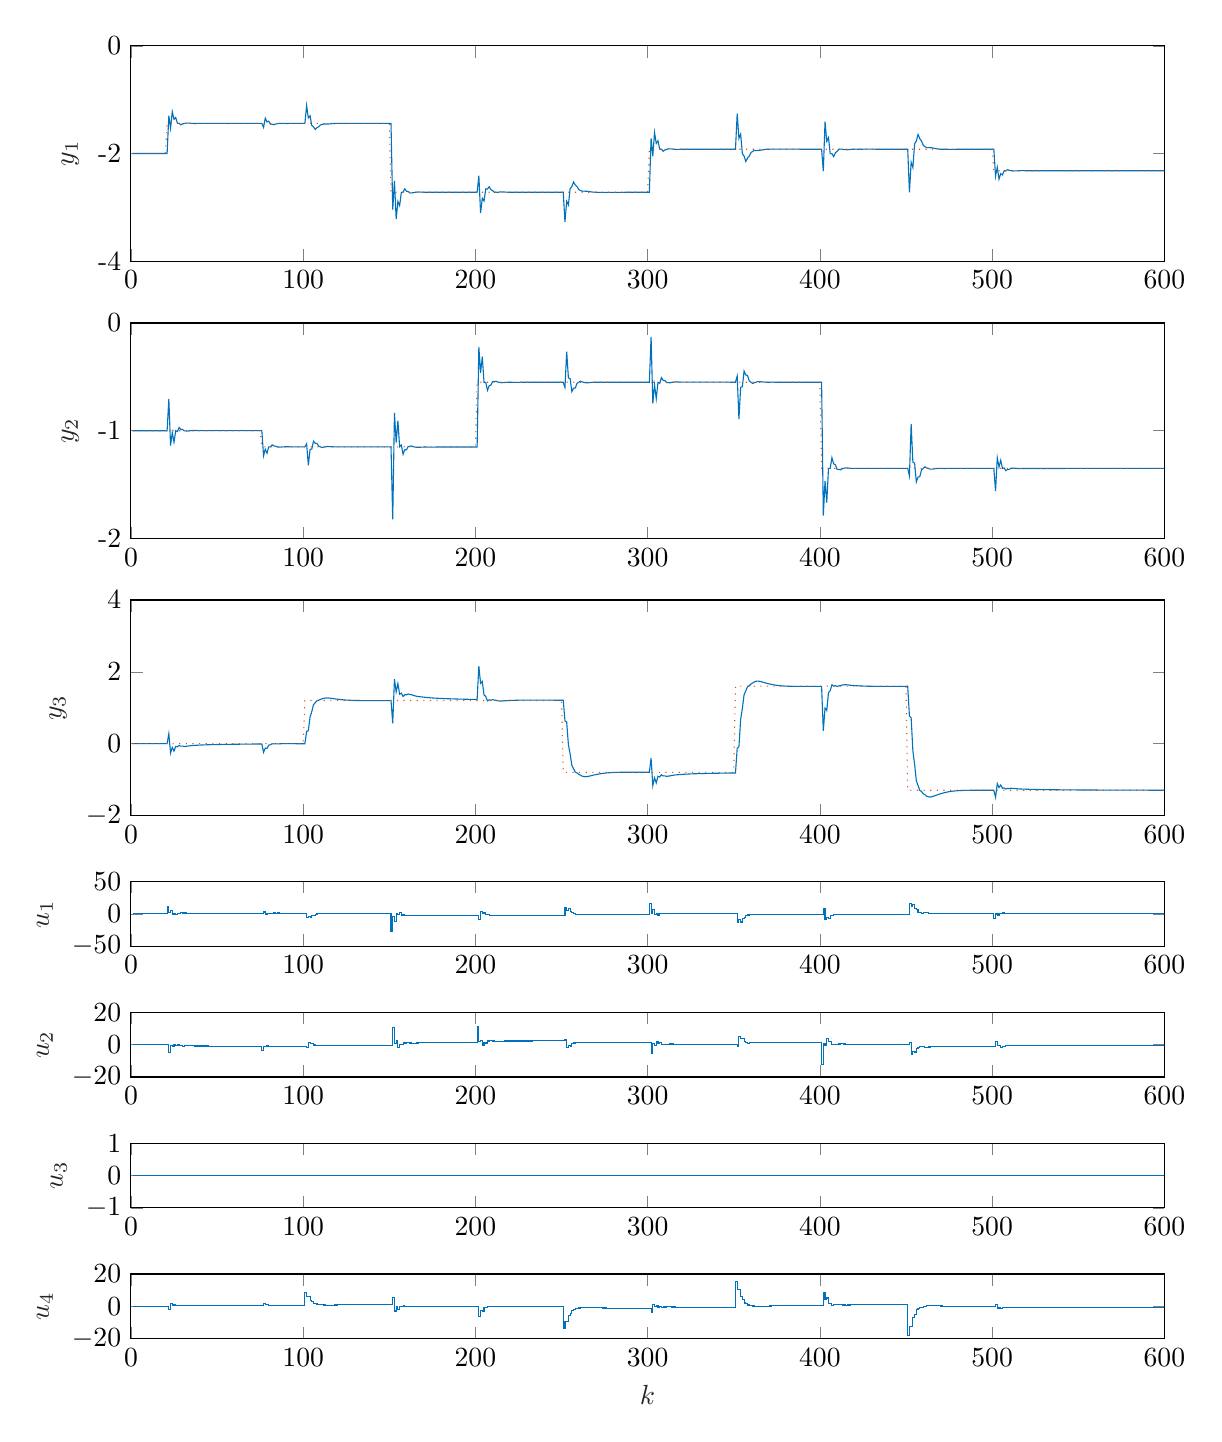
\begin{tikzpicture}

\begin{axis}[%
width=5.167in,
height=0.323in,
at={(0.646in,0.385in)},
scale only axis,
xmin=0,
xmax=600,
xtick={0,100,200,300,400,500,600},
xlabel style={font=\color{white!15!black}},
xlabel={$k$},
ymin=-20,
ymax=20,
ytick={-20,0,20},
ylabel style={font=\color{white!15!black}},
ylabel={$u_4$},
axis background/.style={fill=white}
]
\addplot[const plot, color=mycolor1, forget plot] table[row sep=crcr] {%
1	0\\
2	0\\
3	0\\
4	0\\
5	0\\
6	0\\
7	0\\
8	0\\
9	0\\
10	0\\
11	0\\
12	0\\
13	0\\
14	0\\
15	0\\
16	0\\
17	0\\
18	0\\
19	0\\
20	0\\
21	0\\
22	-1.82172490823151\\
23	1.75101312035058\\
24	0.609925706929148\\
25	1.34708333701041\\
26	0.500768874582458\\
27	0.639211318975843\\
28	0.380571590819368\\
29	0.552273427487523\\
30	0.54195783727685\\
31	0.62981351705284\\
32	0.602441423573711\\
33	0.595483682406782\\
34	0.552125822448342\\
35	0.531610708751532\\
36	0.509906833144299\\
37	0.502348303678034\\
38	0.494337516333856\\
39	0.489289466953646\\
40	0.482069284584296\\
41	0.475384872662732\\
42	0.468549040034285\\
43	0.463090482708527\\
44	0.458634818295361\\
45	0.455356706121562\\
46	0.452744630693287\\
47	0.45065961288293\\
48	0.44886369985727\\
49	0.44733965703521\\
50	0.446040856620482\\
51	0.444974202730137\\
52	0.444104706192417\\
53	0.443402414905135\\
54	0.442823181349544\\
55	0.442334914299205\\
56	0.441910851744406\\
57	0.441535470753438\\
58	0.441197612495475\\
59	0.440890072062394\\
60	0.440606370311292\\
61	0.440341112336507\\
62	0.440089522881418\\
63	0.439848010188037\\
64	0.439614004899836\\
65	0.439385929725733\\
66	0.439162853276377\\
67	0.438944279974931\\
68	0.438729937308742\\
69	0.438519693510038\\
70	0.438313502317582\\
71	0.438111389685867\\
72	0.437913432706275\\
73	0.437719741603358\\
74	0.437530436349492\\
75	0.437345629239296\\
76	0.437165412315544\\
77	1.96601664524842\\
78	1.15494334554056\\
79	1.29645380715553\\
80	0.706306080350899\\
81	0.665828912091718\\
82	0.477207958471878\\
83	0.531505408534388\\
84	0.509264318527634\\
85	0.541078378758743\\
86	0.518836824531683\\
87	0.510399578623853\\
88	0.488352223055916\\
89	0.48183743172793\\
90	0.477773386253472\\
91	0.4822964998482\\
92	0.486949450858888\\
93	0.49269638959984\\
94	0.496698107326802\\
95	0.500260169863273\\
96	0.503088324418543\\
97	0.505977207305075\\
98	0.508747699918079\\
99	0.511482417252448\\
100	0.513937219657188\\
101	8.41313530715394\\
102	6.0065752202299\\
103	6.14143570739524\\
104	3.79439475019079\\
105	3.00656019691298\\
106	1.84433196967543\\
107	1.56971383281226\\
108	1.22450942754574\\
109	1.15913543657902\\
110	0.998096784739681\\
111	0.910510530574867\\
112	0.798062011261584\\
113	0.745581253393019\\
114	0.715168601070218\\
115	0.725540861708184\\
116	0.748712729473407\\
117	0.783331820303418\\
118	0.816603374803143\\
119	0.849363576863832\\
120	0.879044004012455\\
121	0.907406681400315\\
122	0.933807976882156\\
123	0.958522678713138\\
124	0.980802701332399\\
125	1.0004878977304\\
126	1.01735344312674\\
127	1.03160356924635\\
128	1.04347498516331\\
129	1.05331842444117\\
130	1.06141739732541\\
131	1.06803463387722\\
132	1.07337529674147\\
133	1.07762776640802\\
134	1.08095843236227\\
135	1.08352463585753\\
136	1.08546673752341\\
137	1.08690869312051\\
138	1.08795432242619\\
139	1.08868946561713\\
140	1.08918350677731\\
141	1.08949273489171\\
142	1.08966256859305\\
143	1.08972968751142\\
144	1.08972333178212\\
145	1.08966648368865\\
146	1.08957680136965\\
147	1.08946756718455\\
148	1.08934853082773\\
149	1.08922668129831\\
150	1.08910687748217\\
151	1.08899236034602\\
152	5.25282779449778\\
153	-2.91352936206127\\
154	-0.305419524664487\\
155	-1.99043241778828\\
156	-0.0560720970233906\\
157	-0.372576845260356\\
158	0.21854197765691\\
159	-0.173970618046506\\
160	-0.150437673416944\\
161	-0.35129120501427\\
162	-0.288762634405137\\
163	-0.272891711584913\\
164	-0.173817331302831\\
165	-0.126952235391085\\
166	-0.0773676787101071\\
167	-0.0601134086924864\\
168	-0.0418237769894156\\
169	-0.0303047436866414\\
170	-0.0138196735090631\\
171	0.00144176445892219\\
172	0.0170501491764145\\
173	0.0295112016468516\\
174	0.0396805589879638\\
175	0.0471589245884449\\
176	0.0531154168236589\\
177	0.0578676548713853\\
178	0.0619594935554337\\
179	0.0654302968034843\\
180	0.0683866192860295\\
181	0.0708126618587604\\
182	0.0727883851689765\\
183	0.0743822393493962\\
184	0.0756951232606259\\
185	0.0768003800171126\\
186	0.0777591727216876\\
187	0.078606975878608\\
188	0.0793692893792782\\
189	0.0800625758721032\\
190	0.0807016392807832\\
191	0.0812988053531494\\
192	0.0818649835215258\\
193	0.0824083780713172\\
194	0.0829348563476451\\
195	0.0834480180912841\\
196	0.0839499866745669\\
197	0.08444188931513\\
198	0.0849243433705647\\
199	0.0853976445110323\\
200	0.0858618929927455\\
201	0.086317024050901\\
202	-6.02934431613675\\
203	-2.78529829452282\\
204	-3.35157830551786\\
205	-0.991216841416243\\
206	-0.829529215626194\\
207	-0.0752583916995592\\
208	-0.29265346719472\\
209	-0.203887005509797\\
210	-0.331334099162764\\
211	-0.242552009988777\\
212	-0.208980735619083\\
213	-0.120962894163855\\
214	-0.0950694535160982\\
215	-0.0789733946540636\\
216	-0.0972206079398954\\
217	-0.115982028407684\\
218	-0.139114464384311\\
219	-0.15526127463103\\
220	-0.169644904012492\\
221	-0.18108851186449\\
222	-0.192770803898569\\
223	-0.203975457096258\\
224	-0.215033074679895\\
225	-0.224967233947934\\
226	-0.233639327266312\\
227	-0.240799961547123\\
228	-0.246680171017229\\
229	-0.251452691072403\\
230	-0.255370711187215\\
231	-0.258570907045816\\
232	-0.261170004804621\\
233	-0.263233274553404\\
234	-0.264831614341829\\
235	-0.266030386576623\\
236	-0.266901520922916\\
237	-0.267509949314407\\
238	-0.267913498723515\\
239	-0.268157989164693\\
240	-0.268279914839562\\
241	-0.268307527622824\\
242	-0.2682637054348\\
243	-0.268167037687384\\
244	-0.26803287444109\\
245	-0.267873547608273\\
246	-0.267698735662629\\
247	-0.267515731633728\\
248	-0.267329883359804\\
249	-0.267144995355108\\
250	-0.266963720051971\\
251	-13.4285509871751\\
252	-9.41450947722624\\
253	-9.63670821514924\\
254	-5.72287220115063\\
255	-4.40807574764812\\
256	-2.46959497526345\\
257	-2.01072059094144\\
258	-1.43443112588759\\
259	-1.32472446325772\\
260	-1.05574785096792\\
261	-0.909332695835523\\
262	-0.721593801892712\\
263	-0.633890106690736\\
264	-0.583036107986345\\
265	-0.600210991460064\\
266	-0.638760551891441\\
267	-0.696421055370192\\
268	-0.751859956676627\\
269	-0.806464324138222\\
270	-0.855948162120217\\
271	-0.903244013089993\\
272	-0.947276001897644\\
273	-0.98849977948347\\
274	-1.02566686293022\\
275	-1.05850915780151\\
276	-1.08665114217226\\
277	-1.1104326632365\\
278	-1.13024790709008\\
279	-1.14668125966252\\
280	-1.16020518684011\\
281	-1.17125760526367\\
282	-1.18018054224823\\
283	-1.1872880889054\\
284	-1.19285770236131\\
285	-1.19715176553552\\
286	-1.20040435888126\\
287	-1.2028222150496\\
288	-1.20457849731552\\
289	-1.20581639176017\\
290	-1.20665164559876\\
291	-1.20717816868088\\
292	-1.20747174177523\\
293	-1.20759356955681\\
294	-1.20759244741525\\
295	-1.20750673192449\\
296	-1.20736589810352\\
297	-1.20719212106957\\
298	-1.20700168220288\\
299	-1.20680625665292\\
300	-1.20661396510753\\
301	-1.2064302281569\\
302	-3.80872257848362\\
303	1.2953469092387\\
304	-0.334634468180236\\
305	0.718576902128299\\
306	-0.490328572122656\\
307	-0.292451377991847\\
308	-0.661846209895668\\
309	-0.416477942069524\\
310	-0.431143912602152\\
311	-0.305573377535193\\
312	-0.344621012561\\
313	-0.35451134765989\\
314	-0.416407012605992\\
315	-0.445674549378235\\
316	-0.476643994225534\\
317	-0.487408886657071\\
318	-0.49882244458385\\
319	-0.506005680946716\\
320	-0.516293775153662\\
321	-0.525818004942856\\
322	-0.535559836148225\\
323	-0.543335226406724\\
324	-0.549678854409391\\
325	-0.554341084726216\\
326	-0.558052557243464\\
327	-0.561011737778155\\
328	-0.563558499789732\\
329	-0.565717418138445\\
330	-0.567555068324214\\
331	-0.569061559673794\\
332	-0.570286855157135\\
333	-0.571273726493647\\
334	-0.57208522792419\\
335	-0.572767192824745\\
336	-0.573357843085771\\
337	-0.573879345900708\\
338	-0.574347634750932\\
339	-0.574772995076083\\
340	-0.575164675717254\\
341	-0.575530376671819\\
342	-0.575876912700306\\
343	-0.576209407775015\\
344	-0.576531525194951\\
345	-0.576845510918995\\
346	-0.577152688094973\\
347	-0.577453757205234\\
348	-0.577749100015896\\
349	-0.578038897201219\\
350	-0.578323207281257\\
351	15.2155137828698\\
352	10.3985940300501\\
353	10.6651597379937\\
354	5.96848073726874\\
355	4.39064635156636\\
356	2.06438827795841\\
357	1.51365583431663\\
358	0.822023780462828\\
359	0.690290107849402\\
360	0.367432025979609\\
361	0.191647697685013\\
362	-0.0337246853382894\\
363	-0.13905402410171\\
364	-0.200162601858172\\
365	-0.17963512968262\\
366	-0.133456438046302\\
367	-0.064342837895015\\
368	0.00210674513434717\\
369	0.067556885700404\\
370	0.12686445080652\\
371	0.183548527048836\\
372	0.23631807812228\\
373	0.28571988119376\\
374	0.330255738431164\\
375	0.369603906827625\\
376	0.403313721628155\\
377	0.431792954450348\\
378	0.455514578851486\\
379	0.475179804950355\\
380	0.491355536794904\\
381	0.504567218295548\\
382	0.515225225898006\\
383	0.523706412925908\\
384	0.530343672694415\\
385	0.535451810578978\\
386	0.539311670342179\\
387	0.542171279892683\\
388	0.544238385498033\\
389	0.545684762458054\\
390	0.546649261117102\\
391	0.547244528656576\\
392	0.547561459009174\\
393	0.547673456402384\\
394	0.547639035478239\\
395	0.547504185800877\\
396	0.547304240510386\\
397	0.547065774246522\\
398	0.546808290486625\\
399	0.546545766494759\\
400	0.546287915388304\\
401	0.546041211320795\\
402	8.70061924149175\\
403	4.37559208106692\\
404	5.13100473606409\\
405	1.98423341277575\\
406	1.76903082723785\\
407	0.763719565653815\\
408	1.05396357914464\\
409	0.935991418285235\\
410	1.10630173473118\\
411	0.98830285496687\\
412	0.943913567459813\\
413	0.826922984667673\\
414	0.792758186129788\\
415	0.771649098347218\\
416	0.796323012915906\\
417	0.821674086471478\\
418	0.852844430034301\\
419	0.87469166260926\\
420	0.894178943241368\\
421	0.909737127601154\\
422	0.925604530507725\\
423	0.940826147131449\\
424	0.955842915706633\\
425	0.969353105454437\\
426	0.981172096710129\\
427	0.990967573601483\\
428	0.999047802232658\\
429	1.00564332464106\\
430	1.01109195902648\\
431	1.01557617301702\\
432	1.01925183374004\\
433	1.0222061973518\\
434	1.02453401975798\\
435	1.0263226708531\\
436	1.02766827105507\\
437	1.02865760421584\\
438	1.02936797439397\\
439	1.02986066974526\\
440	1.03018453737618\\
441	1.03037742806436\\
442	1.03047002088549\\
443	1.03048727064461\\
444	1.03044980694864\\
445	1.03037422935606\\
446	1.03027359387623\\
447	1.03015777051706\\
448	1.03003403050806\\
449	1.02990758233717\\
450	1.02978209361321\\
451	-18.0548964770714\\
452	-12.2348986994881\\
453	-12.5574327070345\\
454	-6.88269882804198\\
455	-4.97655466176954\\
456	-2.16605097255326\\
457	-1.5009600348955\\
458	-0.665601682702125\\
459	-0.506773917744203\\
460	-0.116991353458259\\
461	0.0950893827079449\\
462	0.367100785362964\\
463	0.494071422913446\\
464	0.567619380063095\\
465	0.542534027748375\\
466	0.486463238059268\\
467	0.402688781236161\\
468	0.322142280323682\\
469	0.242811988553315\\
470	0.170912164516081\\
471	0.102190241869447\\
472	0.0382059081121479\\
473	-0.0217018203323162\\
474	-0.0757228971571074\\
475	-0.123468808917877\\
476	-0.164395246615307\\
477	-0.198995164911923\\
478	-0.22784029187807\\
479	-0.251778130370807\\
480	-0.271493886757083\\
481	-0.287622660687493\\
482	-0.300660503725198\\
483	-0.311062952800181\\
484	-0.319232419582381\\
485	-0.325549453091748\\
486	-0.330353559464185\\
487	-0.333944586802227\\
488	-0.336573704354326\\
489	-0.338448611539232\\
490	-0.339737218800685\\
491	-0.340575769998781\\
492	-0.341074219589404\\
493	-0.341321384584504\\
494	-0.341388086524634\\
495	-0.341330008739185\\
496	-0.341189954438312\\
497	-0.34100014016301\\
498	-0.340784234769366\\
499	-0.340559226353124\\
500	-0.340336947352241\\
501	-0.340125313410186\\
502	0.96130280041576\\
503	-1.59047523507708\\
504	-0.775254549560944\\
505	-1.3016568778092\\
506	-0.697026297791566\\
507	-0.795810774764891\\
508	-0.610980796863918\\
509	-0.733551601095692\\
510	-0.726122179002508\\
511	-0.788825648587303\\
512	-0.769232566213307\\
513	-0.764228745987836\\
514	-0.733231154800538\\
515	-0.718555010374509\\
516	-0.703033984873422\\
517	-0.697620188577755\\
518	-0.691886066483063\\
519	-0.688270322107569\\
520	-0.683104713280678\\
521	-0.678323068104406\\
522	-0.673434222979901\\
523	-0.669529855045857\\
524	-0.666342353406672\\
525	-0.663996324194598\\
526	-0.662126284925663\\
527	-0.660632879793929\\
528	-0.659346080835125\\
529	-0.658253534354035\\
530	-0.657321905756614\\
531	-0.656556108409054\\
532	-0.655931140044555\\
533	-0.655425602258392\\
534	-0.655007961286452\\
535	-0.654655297875386\\
536	-0.654348501191385\\
537	-0.654076489367175\\
538	-0.653831298226306\\
539	-0.653607787883491\\
540	-0.653401336629792\\
541	-0.653208096794191\\
542	-0.653024662779536\\
543	-0.652848473752336\\
544	-0.652677698553716\\
545	-0.652511214039547\\
546	-0.652348357848501\\
547	-0.652188778378187\\
548	-0.652032282868735\\
549	-0.651878778652856\\
550	-0.651728233749605\\
551	-0.651580667418942\\
552	-0.651436135150469\\
553	-0.651294715845034\\
554	-0.651156495148296\\
555	-0.651021553037183\\
556	-0.650889954867699\\
557	-0.650761747701805\\
558	-0.650636959540969\\
559	-0.650515600545783\\
560	-0.65039766467137\\
561	-0.650283131408888\\
562	-0.650171967371015\\
563	-0.650064127889234\\
564	-0.64995955863459\\
565	-0.649858197287465\\
566	-0.649759975165193\\
567	-0.649664818738139\\
568	-0.649572650968812\\
569	-0.649483392458346\\
570	-0.649396962405848\\
571	-0.649313279404906\\
572	-0.649232262100237\\
573	-0.649153829724974\\
574	-0.649077902533254\\
575	-0.64900440214064\\
576	-0.648933251783793\\
577	-0.64886437651109\\
578	-0.648797703315652\\
579	-0.648733161221596\\
580	-0.648670681332929\\
581	-0.648610196853017\\
582	-0.648551643081112\\
583	-0.648494957391183\\
584	-0.64844007919736\\
585	-0.648386949909548\\
586	-0.648335512882112\\
587	-0.648285713357965\\
588	-0.648237498409961\\
589	-0.648190816880986\\
590	-0.648145619323836\\
591	-0.648101857941678\\
592	-0.648059486529646\\
593	-0.648018460417984\\
594	-0.647978736416965\\
595	-0.64794027276378\\
596	-0.647903029071431\\
597	-0.647866966279675\\
598	-0.647832046608011\\
599	-0.647798233510634\\
600	-0.647765491633278\\
};
\end{axis}

\begin{axis}[%
width=5.167in,
height=0.323in,
at={(0.646in,1.039in)},
scale only axis,
xmin=0,
xmax=600,
xtick={0,100,200,300,400,500,600},
ymin=-1,
ymax=1,
ytick={-1,0,1},
ylabel style={font=\color{white!15!black}},
ylabel={$u_3$},
axis background/.style={fill=white}
]
\addplot[const plot, color=mycolor1, forget plot] table[row sep=crcr] {%
1	0\\
2	0\\
3	0\\
4	0\\
5	0\\
6	0\\
7	0\\
8	0\\
9	0\\
10	0\\
11	0\\
12	0\\
13	0\\
14	0\\
15	0\\
16	0\\
17	0\\
18	0\\
19	0\\
20	0\\
21	0\\
22	0\\
23	0\\
24	0\\
25	0\\
26	0\\
27	0\\
28	0\\
29	0\\
30	0\\
31	0\\
32	0\\
33	0\\
34	0\\
35	0\\
36	0\\
37	0\\
38	0\\
39	0\\
40	0\\
41	0\\
42	0\\
43	0\\
44	0\\
45	0\\
46	0\\
47	0\\
48	0\\
49	0\\
50	0\\
51	0\\
52	0\\
53	0\\
54	0\\
55	0\\
56	0\\
57	0\\
58	0\\
59	0\\
60	0\\
61	0\\
62	0\\
63	0\\
64	0\\
65	0\\
66	0\\
67	0\\
68	0\\
69	0\\
70	0\\
71	0\\
72	0\\
73	0\\
74	0\\
75	0\\
76	0\\
77	0\\
78	0\\
79	0\\
80	0\\
81	0\\
82	0\\
83	0\\
84	0\\
85	0\\
86	0\\
87	0\\
88	0\\
89	0\\
90	0\\
91	0\\
92	0\\
93	0\\
94	0\\
95	0\\
96	0\\
97	0\\
98	0\\
99	0\\
100	0\\
101	0\\
102	0\\
103	0\\
104	0\\
105	0\\
106	0\\
107	0\\
108	0\\
109	0\\
110	0\\
111	0\\
112	0\\
113	0\\
114	0\\
115	0\\
116	0\\
117	0\\
118	0\\
119	0\\
120	0\\
121	0\\
122	0\\
123	0\\
124	0\\
125	0\\
126	0\\
127	0\\
128	0\\
129	0\\
130	0\\
131	0\\
132	0\\
133	0\\
134	0\\
135	0\\
136	0\\
137	0\\
138	0\\
139	0\\
140	0\\
141	0\\
142	0\\
143	0\\
144	0\\
145	0\\
146	0\\
147	0\\
148	0\\
149	0\\
150	0\\
151	0\\
152	0\\
153	0\\
154	0\\
155	0\\
156	0\\
157	0\\
158	0\\
159	0\\
160	0\\
161	0\\
162	0\\
163	0\\
164	0\\
165	0\\
166	0\\
167	0\\
168	0\\
169	0\\
170	0\\
171	0\\
172	0\\
173	0\\
174	0\\
175	0\\
176	0\\
177	0\\
178	0\\
179	0\\
180	0\\
181	0\\
182	0\\
183	0\\
184	0\\
185	0\\
186	0\\
187	0\\
188	0\\
189	0\\
190	0\\
191	0\\
192	0\\
193	0\\
194	0\\
195	0\\
196	0\\
197	0\\
198	0\\
199	0\\
200	0\\
201	0\\
202	0\\
203	0\\
204	0\\
205	0\\
206	0\\
207	0\\
208	0\\
209	0\\
210	0\\
211	0\\
212	0\\
213	0\\
214	0\\
215	0\\
216	0\\
217	0\\
218	0\\
219	0\\
220	0\\
221	0\\
222	0\\
223	0\\
224	0\\
225	0\\
226	0\\
227	0\\
228	0\\
229	0\\
230	0\\
231	0\\
232	0\\
233	0\\
234	0\\
235	0\\
236	0\\
237	0\\
238	0\\
239	0\\
240	0\\
241	0\\
242	0\\
243	0\\
244	0\\
245	0\\
246	0\\
247	0\\
248	0\\
249	0\\
250	0\\
251	0\\
252	0\\
253	0\\
254	0\\
255	0\\
256	0\\
257	0\\
258	0\\
259	0\\
260	0\\
261	0\\
262	0\\
263	0\\
264	0\\
265	0\\
266	0\\
267	0\\
268	0\\
269	0\\
270	0\\
271	0\\
272	0\\
273	0\\
274	0\\
275	0\\
276	0\\
277	0\\
278	0\\
279	0\\
280	0\\
281	0\\
282	0\\
283	0\\
284	0\\
285	0\\
286	0\\
287	0\\
288	0\\
289	0\\
290	0\\
291	0\\
292	0\\
293	0\\
294	0\\
295	0\\
296	0\\
297	0\\
298	0\\
299	0\\
300	0\\
301	0\\
302	0\\
303	0\\
304	0\\
305	0\\
306	0\\
307	0\\
308	0\\
309	0\\
310	0\\
311	0\\
312	0\\
313	0\\
314	0\\
315	0\\
316	0\\
317	0\\
318	0\\
319	0\\
320	0\\
321	0\\
322	0\\
323	0\\
324	0\\
325	0\\
326	0\\
327	0\\
328	0\\
329	0\\
330	0\\
331	0\\
332	0\\
333	0\\
334	0\\
335	0\\
336	0\\
337	0\\
338	0\\
339	0\\
340	0\\
341	0\\
342	0\\
343	0\\
344	0\\
345	0\\
346	0\\
347	0\\
348	0\\
349	0\\
350	0\\
351	0\\
352	0\\
353	0\\
354	0\\
355	0\\
356	0\\
357	0\\
358	0\\
359	0\\
360	0\\
361	0\\
362	0\\
363	0\\
364	0\\
365	0\\
366	0\\
367	0\\
368	0\\
369	0\\
370	0\\
371	0\\
372	0\\
373	0\\
374	0\\
375	0\\
376	0\\
377	0\\
378	0\\
379	0\\
380	0\\
381	0\\
382	0\\
383	0\\
384	0\\
385	0\\
386	0\\
387	0\\
388	0\\
389	0\\
390	0\\
391	0\\
392	0\\
393	0\\
394	0\\
395	0\\
396	0\\
397	0\\
398	0\\
399	0\\
400	0\\
401	0\\
402	0\\
403	0\\
404	0\\
405	0\\
406	0\\
407	0\\
408	0\\
409	0\\
410	0\\
411	0\\
412	0\\
413	0\\
414	0\\
415	0\\
416	0\\
417	0\\
418	0\\
419	0\\
420	0\\
421	0\\
422	0\\
423	0\\
424	0\\
425	0\\
426	0\\
427	0\\
428	0\\
429	0\\
430	0\\
431	0\\
432	0\\
433	0\\
434	0\\
435	0\\
436	0\\
437	0\\
438	0\\
439	0\\
440	0\\
441	0\\
442	0\\
443	0\\
444	0\\
445	0\\
446	0\\
447	0\\
448	0\\
449	0\\
450	0\\
451	0\\
452	0\\
453	0\\
454	0\\
455	0\\
456	0\\
457	0\\
458	0\\
459	0\\
460	0\\
461	0\\
462	0\\
463	0\\
464	0\\
465	0\\
466	0\\
467	0\\
468	0\\
469	0\\
470	0\\
471	0\\
472	0\\
473	0\\
474	0\\
475	0\\
476	0\\
477	0\\
478	0\\
479	0\\
480	0\\
481	0\\
482	0\\
483	0\\
484	0\\
485	0\\
486	0\\
487	0\\
488	0\\
489	0\\
490	0\\
491	0\\
492	0\\
493	0\\
494	0\\
495	0\\
496	0\\
497	0\\
498	0\\
499	0\\
500	0\\
501	0\\
502	0\\
503	0\\
504	0\\
505	0\\
506	0\\
507	0\\
508	0\\
509	0\\
510	0\\
511	0\\
512	0\\
513	0\\
514	0\\
515	0\\
516	0\\
517	0\\
518	0\\
519	0\\
520	0\\
521	0\\
522	0\\
523	0\\
524	0\\
525	0\\
526	0\\
527	0\\
528	0\\
529	0\\
530	0\\
531	0\\
532	0\\
533	0\\
534	0\\
535	0\\
536	0\\
537	0\\
538	0\\
539	0\\
540	0\\
541	0\\
542	0\\
543	0\\
544	0\\
545	0\\
546	0\\
547	0\\
548	0\\
549	0\\
550	0\\
551	0\\
552	0\\
553	0\\
554	0\\
555	0\\
556	0\\
557	0\\
558	0\\
559	0\\
560	0\\
561	0\\
562	0\\
563	0\\
564	0\\
565	0\\
566	0\\
567	0\\
568	0\\
569	0\\
570	0\\
571	0\\
572	0\\
573	0\\
574	0\\
575	0\\
576	0\\
577	0\\
578	0\\
579	0\\
580	0\\
581	0\\
582	0\\
583	0\\
584	0\\
585	0\\
586	0\\
587	0\\
588	0\\
589	0\\
590	0\\
591	0\\
592	0\\
593	0\\
594	0\\
595	0\\
596	0\\
597	0\\
598	0\\
599	0\\
600	0\\
};
\end{axis}

\begin{axis}[%
width=5.167in,
height=0.323in,
at={(0.646in,1.693in)},
scale only axis,
xmin=0,
xmax=600,
xtick={0,100,200,300,400,500,600},
ymin=-20,
ymax=20,
ytick={-20,0,20},
ylabel style={font=\color{white!15!black}},
ylabel={$u_2$},
axis background/.style={fill=white}
]
\addplot[const plot, color=mycolor1, forget plot] table[row sep=crcr] {%
1	0\\
2	0\\
3	0\\
4	0\\
5	0\\
6	0\\
7	0\\
8	0\\
9	0\\
10	0\\
11	0\\
12	0\\
13	0\\
14	0\\
15	0\\
16	0\\
17	0\\
18	0\\
19	0\\
20	0\\
21	0\\
22	-4.85033194635755\\
23	-0.659148130423113\\
24	-1.27556180957703\\
25	0.370029059970629\\
26	-0.32141621534947\\
27	-0.204953153478433\\
28	-0.745938913189874\\
29	-0.746024264266213\\
30	-0.858843917667978\\
31	-0.750339840275028\\
32	-0.730155953578437\\
33	-0.682474162331538\\
34	-0.701240261979573\\
35	-0.716313573928885\\
36	-0.746675171868968\\
37	-0.76270599923678\\
38	-0.77602155035802\\
39	-0.781674715215187\\
40	-0.788016926992489\\
41	-0.794233740156707\\
42	-0.802558944151519\\
43	-0.811284071348673\\
44	-0.820270587802847\\
45	-0.828580475434204\\
46	-0.836338027792352\\
47	-0.843516294874763\\
48	-0.850405419921614\\
49	-0.857085489517523\\
50	-0.863640274388665\\
51	-0.870033398923848\\
52	-0.87624394411464\\
53	-0.882240152760427\\
54	-0.888023502626902\\
55	-0.893602328472133\\
56	-0.898994977000976\\
57	-0.904214511579202\\
58	-0.909270937165797\\
59	-0.914169152202645\\
60	-0.918912986837231\\
61	-0.923505878463984\\
62	-0.927952286608336\\
63	-0.932257152381105\\
64	-0.936425682584008\\
65	-0.940462786315966\\
66	-0.944372997096109\\
67	-0.948160443556913\\
68	-0.951829004880309\\
69	-0.955382400167382\\
70	-0.958824260543926\\
71	-0.962158130120542\\
72	-0.96538745553119\\
73	-0.968515566132872\\
74	-0.971545669564219\\
75	-0.974480854997715\\
76	-3.44900111584903\\
77	-1.11596371385135\\
78	-1.2939680513045\\
79	-0.459951742333504\\
80	-0.850516666780339\\
81	-0.852815682277192\\
82	-1.16115674513822\\
83	-1.17435384795194\\
84	-1.22551080538645\\
85	-1.16134729497606\\
86	-1.14366194385359\\
87	-1.11735579969206\\
88	-1.12745710843906\\
89	-1.136530886208\\
90	-1.15213994656046\\
91	-1.15906260844582\\
92	-1.16346029598552\\
93	-1.16357116496024\\
94	-1.16406324083707\\
95	-1.1647456730391\\
96	-1.16670067110002\\
97	-1.16896343937424\\
98	-1.17136840425593\\
99	-1.1734164116869\\
100	-1.17518659213702\\
101	-1.17670275838378\\
102	-1.65411552797268\\
103	1.35063935833962\\
104	0.631333012516475\\
105	0.808629698425976\\
106	-0.180385739772845\\
107	-0.388991545158168\\
108	-0.696816246570749\\
109	-0.586712580017102\\
110	-0.549949361347718\\
111	-0.452623183441572\\
112	-0.460696577776777\\
113	-0.476936648105601\\
114	-0.525122408118132\\
115	-0.553185583481729\\
116	-0.573065627090836\\
117	-0.57600155153276\\
118	-0.575895338769638\\
119	-0.57380599054029\\
120	-0.574790166190378\\
121	-0.577029665231669\\
122	-0.580299106416901\\
123	-0.582886322846178\\
124	-0.584718700212055\\
125	-0.585681959070004\\
126	-0.586284293443003\\
127	-0.586773166038939\\
128	-0.587376164199391\\
129	-0.588085656767897\\
130	-0.588869644298737\\
131	-0.589656729975157\\
132	-0.590422927524881\\
133	-0.591162259368037\\
134	-0.59189174833673\\
135	-0.592624371739568\\
136	-0.593368260758158\\
137	-0.594121727518062\\
138	-0.594879497380261\\
139	-0.595634941422158\\
140	-0.596383377098179\\
141	-0.597121895040403\\
142	-0.597849111478505\\
143	-0.598564096122633\\
144	-0.599265979630595\\
145	-0.599953730839421\\
146	-0.600626326105201\\
147	-0.601282888131781\\
148	-0.601922810578628\\
149	-0.602545755378178\\
150	-0.603151607092225\\
151	-0.603740398756277\\
152	10.4821607602302\\
153	0.901756913410615\\
154	2.31016383128294\\
155	-1.45170916510131\\
156	0.12823060302643\\
157	-0.138461763580547\\
158	1.09760113375756\\
159	1.0973349332416\\
160	1.35476141791912\\
161	1.10631895495569\\
162	1.0597646676611\\
163	0.950371074784218\\
164	0.992871023480798\\
165	1.02694257129929\\
166	1.09597064745335\\
167	1.13225417929231\\
168	1.16234250687535\\
169	1.17492759984314\\
170	1.18909810898368\\
171	1.20299211601281\\
172	1.22171510751973\\
173	1.24136170716072\\
174	1.26161496851595\\
175	1.28033056261888\\
176	1.29779231080198\\
177	1.31393834394653\\
178	1.3294315862501\\
179	1.34445484084445\\
180	1.35919933987051\\
181	1.37358170307841\\
182	1.38755388711406\\
183	1.40104308285423\\
184	1.41405245379199\\
185	1.42660084327578\\
186	1.43872998559724\\
187	1.45046954511323\\
188	1.46184220159198\\
189	1.47285896861503\\
190	1.48352842360716\\
191	1.49385825174627\\
192	1.50385847980758\\
193	1.51354024046176\\
194	1.52291527863958\\
195	1.53199466361901\\
196	1.54078861087066\\
197	1.54930641492611\\
198	1.557556804521\\
199	1.56554814673396\\
200	1.57328861166915\\
201	11.4674942229668\\
202	2.13159025192715\\
203	2.83997063134652\\
204	-0.499617785750264\\
205	1.05922898698288\\
206	1.06511893444562\\
207	2.29528053665095\\
208	2.3449665258203\\
209	2.54658902743725\\
210	2.28702371796243\\
211	2.21346216565482\\
212	2.10550571011144\\
213	2.14326457055184\\
214	2.17699613176622\\
215	2.23694905166847\\
216	2.26223409116026\\
217	2.27749451095634\\
218	2.27568057502245\\
219	2.27546210016187\\
220	2.27607347069744\\
221	2.28184138083821\\
222	2.28890457138478\\
223	2.29659873654084\\
224	2.30292531192424\\
225	2.30819893250486\\
226	2.31251302178408\\
227	2.31656485188892\\
228	2.32056777431379\\
229	2.32468437632094\\
230	2.32881109972721\\
231	2.3328738504449\\
232	2.33678834115168\\
233	2.34054754432504\\
234	2.34416357454198\\
235	2.34766831120015\\
236	2.35108033786811\\
237	2.35440945983803\\
238	2.35765413369599\\
239	2.36081097447445\\
240	2.3638769021756\\
241	2.3668520457078\\
242	2.36973837868472\\
243	2.37253894536429\\
244	2.37525652713965\\
245	2.37789342630366\\
246	2.38045143665312\\
247	2.38293219631551\\
248	2.38533738156226\\
249	2.3876688312227\\
250	2.38992850904356\\
251	2.392118440453\\
252	3.18753373404803\\
253	-1.8206870166567\\
254	-0.622228851167007\\
255	-0.918154522994616\\
256	0.729759956613427\\
257	1.077014625038\\
258	1.58966112368816\\
259	1.40578344381163\\
260	1.34415078267442\\
261	1.18158414418026\\
262	1.19468472447892\\
263	1.22139937243616\\
264	1.3013621915134\\
265	1.347794982539\\
266	1.38059772608138\\
267	1.38516887186763\\
268	1.38467801108386\\
269	1.38088984980791\\
270	1.38223202944338\\
271	1.38567427728951\\
272	1.39084105875456\\
273	1.3948788225487\\
274	1.39766651334353\\
275	1.39901355864708\\
276	1.39976679355322\\
277	1.40033848409228\\
278	1.40110776788425\\
279	1.40206175327951\\
280	1.40314693307034\\
281	1.40424413323124\\
282	1.40531319176363\\
283	1.40634395734762\\
284	1.40736461151358\\
285	1.40839659467392\\
286	1.40945327345006\\
287	1.41053165330847\\
288	1.4116227659861\\
289	1.41271539037946\\
290	1.41380155372176\\
291	1.41487624305098\\
292	1.4159369927172\\
293	1.41698209762012\\
294	1.41800995901142\\
295	1.41901871316722\\
296	1.42000651352396\\
297	1.4209717619374\\
298	1.4219133162319\\
299	1.42283048559843\\
300	1.42372295439192\\
301	1.42459065840851\\
302	-5.50361193933847\\
303	0.484612099157186\\
304	-0.395184434117987\\
305	1.95643033591697\\
306	0.969398732828458\\
307	1.13649910480258\\
308	0.364364641918274\\
309	0.364923402374308\\
310	0.204412113437862\\
311	0.360057140992388\\
312	0.389510628189979\\
313	0.458227593324622\\
314	0.432000344869782\\
315	0.411030428726479\\
316	0.368202588694117\\
317	0.345830311476874\\
318	0.327320566941637\\
319	0.319741172232141\\
320	0.311162009435596\\
321	0.302747057027166\\
322	0.291305656311796\\
323	0.279278929018511\\
324	0.26686521951466\\
325	0.255404977872007\\
326	0.244721052124961\\
327	0.234852339034573\\
328	0.225384732030489\\
329	0.216204192991776\\
330	0.207191408732741\\
331	0.198398692148354\\
332	0.189856264167215\\
333	0.181609818160583\\
334	0.173657558681735\\
335	0.165987884659327\\
336	0.158574882673342\\
337	0.15140017769857\\
338	0.144449754947563\\
339	0.13771688604409\\
340	0.131196360420277\\
341	0.124883520530671\\
342	0.118772240850009\\
343	0.112855700330568\\
344	0.107126691061832\\
345	0.101578423347975\\
346	0.0962046371812987\\
347	0.090999644321505\\
348	0.0859581064488792\\
349	0.0810749076909452\\
350	0.0763450518054858\\
351	0.0717636609936488\\
352	-0.884625722907889\\
353	5.12340836942832\\
354	3.68348587227625\\
355	4.0368800889865\\
356	2.0577203393684\\
357	1.63940478329701\\
358	1.02266974046237\\
359	1.24181278387685\\
360	1.31430930324339\\
361	1.50797257853294\\
362	1.49087971332215\\
363	1.45749307937115\\
364	1.36025039161899\\
365	1.30328417419529\\
366	1.26271317898628\\
367	1.25605803603874\\
368	1.2555140448357\\
369	1.25896240454449\\
370	1.25628882809878\\
371	1.25112856027499\\
372	1.24393119388595\\
373	1.23811997446078\\
374	1.23383918401473\\
375	1.2313165558104\\
376	1.22953496371699\\
377	1.22799879329117\\
378	1.22625221213024\\
379	1.22430985006917\\
380	1.22223510191633\\
381	1.22017018817571\\
382	1.21816253966339\\
383	1.216223598375\\
384	1.21431883014854\\
385	1.21242181271403\\
386	1.2105158342075\\
387	1.20860383733259\\
388	1.20669595379279\\
389	1.2048050385854\\
390	1.20294006796737\\
391	1.20110648508983\\
392	1.19930669440278\\
393	1.19754220520084\\
394	1.19581441610814\\
395	1.19412506013567\\
396	1.19247586559891\\
397	1.19086827810359\\
398	1.18930321099881\\
399	1.18778105042681\\
400	1.18630174630838\\
401	-11.9974124375558\\
402	0.458747955759925\\
403	-0.477732971383783\\
404	3.98282452651239\\
405	1.91189024169557\\
406	1.91132823439745\\
407	0.278174882593786\\
408	0.218767247707354\\
409	-0.0434370820644759\\
410	0.309067820684372\\
411	0.413366451105381\\
412	0.563330046194344\\
413	0.518817785960058\\
414	0.479492423819415\\
415	0.405028153975224\\
416	0.376616181239917\\
417	0.361404200275953\\
418	0.36879706487955\\
419	0.373906728183363\\
420	0.37775889546587\\
421	0.374589372970541\\
422	0.369551090639102\\
423	0.363534231111752\\
424	0.359207850225442\\
425	0.35615660405975\\
426	0.354259967469986\\
427	0.352592157905483\\
428	0.350872498228233\\
429	0.348887878536\\
430	0.346779934698264\\
431	0.344650905787706\\
432	0.342616513911097\\
433	0.340689363461573\\
434	0.338856434593551\\
435	0.337078256047898\\
436	0.335332989052399\\
437	0.333610406868255\\
438	0.331915324897055\\
439	0.330254927263621\\
440	0.328635907490673\\
441	0.327060599210446\\
442	0.325528797648498\\
443	0.324038794178264\\
444	0.322589156731745\\
445	0.321179020439148\\
446	0.319808129077786\\
447	0.318476366821242\\
448	0.317183501938975\\
449	0.315929022962162\\
450	0.31471219085809\\
451	0.313532125269487\\
452	1.46266289198643\\
453	-5.8033483234014\\
454	-4.06954851022108\\
455	-4.50248227496623\\
456	-2.11672840100587\\
457	-1.61681536369824\\
458	-0.876971765912297\\
459	-1.14697924134478\\
460	-1.23962579803406\\
461	-1.47852423852742\\
462	-1.46260599717736\\
463	-1.42685122267055\\
464	-1.31379345667779\\
465	-1.24926399321305\\
466	-1.20441068011809\\
467	-1.20040850021803\\
468	-1.20366419751422\\
469	-1.21162151718181\\
470	-1.21206286783139\\
471	-1.20938455535732\\
472	-1.20413343951917\\
473	-1.20044943071082\\
474	-1.19851024885864\\
475	-1.19859434465749\\
476	-1.19947586084581\\
477	-1.20055900047218\\
478	-1.20129594003237\\
479	-1.20170723775031\\
480	-1.20187228567257\\
481	-1.20196563590648\\
482	-1.20204721813998\\
483	-1.20213339337576\\
484	-1.20218488849835\\
485	-1.20217215518387\\
486	-1.20207730387362\\
487	-1.2019061219939\\
488	-1.20167301367733\\
489	-1.20139560591019\\
490	-1.20108677321234\\
491	-1.20075505734795\\
492	-1.20040526673386\\
493	-1.20004106849579\\
494	-1.1996659382642\\
495	-1.19928369976863\\
496	-1.19889811687201\\
497	-1.1985125593398\\
498	-1.198129702953\\
499	-1.19775153720661\\
500	-1.19737947679641\\
501	-1.1970145419784\\
502	2.26786533379982\\
503	-0.72548877652956\\
504	-0.284853522107476\\
505	-1.45994490855067\\
506	-0.965733997336394\\
507	-1.04860972166695\\
508	-0.661888327766739\\
509	-0.661533420678731\\
510	-0.58066289099671\\
511	-0.657889418655672\\
512	-0.672038554779239\\
513	-0.705837279178041\\
514	-0.692181214198919\\
515	-0.681170603581882\\
516	-0.659247297049013\\
517	-0.647567526259114\\
518	-0.637834277386567\\
519	-0.633580974702362\\
520	-0.628842090180169\\
521	-0.624199159472289\\
522	-0.618056415057447\\
523	-0.611633994772356\\
524	-0.605030662533444\\
525	-0.59891624940326\\
526	-0.593201799194586\\
527	-0.587906393290269\\
528	-0.582822624036097\\
529	-0.5778931300568\\
530	-0.573057923943208\\
531	-0.56834284229711\\
532	-0.563762686211965\\
533	-0.559340003014497\\
534	-0.555073605203338\\
535	-0.550957411644845\\
536	-0.546978193838561\\
537	-0.54312650094283\\
538	-0.539395070374479\\
539	-0.535780290595918\\
540	-0.532279316534047\\
541	-0.52888958692541\\
542	-0.525607813568973\\
543	-0.522430367322665\\
544	-0.519353432213417\\
545	-0.51637340776712\\
546	-0.513486964546322\\
547	-0.510691064999601\\
548	-0.507982852355755\\
549	-0.505359586711828\\
550	-0.502818593455779\\
551	-0.500357262510115\\
552	-0.497973055736247\\
553	-0.495663521011732\\
554	-0.493426295338913\\
555	-0.491259102460018\\
556	-0.489159745226457\\
557	-0.487126098729701\\
558	-0.485156104925849\\
559	-0.483247769716716\\
560	-0.481399161146573\\
561	-0.479608408067682\\
562	-0.477873698536156\\
563	-0.476193277942067\\
564	-0.474565446955227\\
565	-0.472988559525413\\
566	-0.471461021029674\\
567	-0.469981286601318\\
568	-0.46854785958809\\
569	-0.467159290089994\\
570	-0.465814173535399\\
571	-0.464511149284429\\
572	-0.463248899261549\\
573	-0.462026146626477\\
574	-0.460841654488483\\
575	-0.459694224665073\\
576	-0.458582696482008\\
577	-0.457505945610871\\
578	-0.456462882941049\\
579	-0.455452453484398\\
580	-0.454473635311838\\
581	-0.453525438521527\\
582	-0.452606904238246\\
583	-0.451717103643344\\
584	-0.450855137034442\\
585	-0.450020132913962\\
586	-0.449211247105635\\
587	-0.448427661898153\\
588	-0.447668585215236\\
589	-0.446933249811411\\
590	-0.446220912492779\\
591	-0.445530853362079\\
592	-0.444862375087328\\
593	-0.444214802193348\\
594	-0.443587480375504\\
595	-0.442979775834945\\
596	-0.442391074634726\\
597	-0.441820782076147\\
598	-0.441268322094698\\
599	-0.440733136675011\\
600	-0.440214685284225\\
};
\end{axis}

\begin{axis}[%
width=5.167in,
height=0.323in,
at={(0.646in,2.347in)},
scale only axis,
xmin=0,
xmax=600,
xtick={0,100,200,300,400,500,600},
ymin=-50,
ymax=50,
ytick={-50,0,50},
ylabel style={font=\color{white!15!black}},
ylabel={$u_1$},
axis background/.style={fill=white}
]
\addplot[const plot, color=mycolor1, forget plot] table[row sep=crcr] {%
1	0\\
2	0\\
3	0\\
4	0\\
5	0\\
6	0\\
7	0\\
8	0\\
9	0\\
10	0\\
11	0\\
12	0\\
13	0\\
14	0\\
15	0\\
16	0\\
17	0\\
18	0\\
19	0\\
20	0\\
21	12.0211877448499\\
22	1.73548313158956\\
23	5.53338173001506\\
24	-0.331024873400251\\
25	0.886693493132278\\
26	-0.475383406781415\\
27	0.909224803714707\\
28	0.921493250134384\\
29	1.51340829467764\\
30	1.33829506990413\\
31	1.34531787427236\\
32	1.15313688239586\\
33	1.13523320404753\\
34	1.10671837768049\\
35	1.15644341402605\\
36	1.18406919901257\\
37	1.2163682281281\\
38	1.22424690851037\\
39	1.22943711113623\\
40	1.22868436921029\\
41	1.2321474597798\\
42	1.23693354548082\\
43	1.24419656815844\\
44	1.25100848372304\\
45	1.25724545272633\\
46	1.26215788720613\\
47	1.26633011144549\\
48	1.2699576439282\\
49	1.27344198714772\\
50	1.27681733515656\\
51	1.28011365387639\\
52	1.28324802558966\\
53	1.28619945702194\\
54	1.28895575577004\\
55	1.29154779687607\\
56	1.29400431649514\\
57	1.29635453168018\\
58	1.29861328204768\\
59	1.30078913262133\\
60	1.30288502621193\\
61	1.30490417528437\\
62	1.30685020949072\\
63	1.30872794054577\\
64	1.31054204803056\\
65	1.31229671742597\\
66	1.31399518406523\\
67	1.31563996859283\\
68	1.31723307783202\\
69	1.31877629975381\\
70	1.32027131654415\\
71	1.32171976083803\\
72	1.32312319135889\\
73	1.32448307798902\\
74	1.32580079243295\\
75	1.32707762258755\\
76	1.32831479121448\\
77	2.97260854403643\\
78	-0.0795699116465198\\
79	0.574921974822903\\
80	0.0614172065131667\\
81	0.920758638121379\\
82	1.04949234564\\
83	1.40427606169664\\
84	1.3359347886463\\
85	1.34048050317094\\
86	1.24594042882262\\
87	1.2432649977708\\
88	1.2387982148078\\
89	1.27236779457667\\
90	1.29130974683044\\
91	1.30837295083313\\
92	1.31026465676273\\
93	1.3093661275162\\
94	1.30527967301055\\
95	1.30360550967223\\
96	1.30296896112778\\
97	1.30379061269551\\
98	1.30447795826378\\
99	1.30492886734465\\
100	1.30481451390965\\
101	1.30449531925169\\
102	-5.79400347635676\\
103	-3.66239958115351\\
104	-5.38642308948869\\
105	-2.68777166908121\\
106	-1.85736178525922\\
107	-0.229012776877122\\
108	0.0362437631500572\\
109	0.341232718493659\\
110	0.187302161314699\\
111	0.217843060410391\\
112	0.215024877650542\\
113	0.332927799322779\\
114	0.418761763988415\\
115	0.501925536966873\\
116	0.532098103661127\\
117	0.541702707727521\\
118	0.530605615512362\\
119	0.519806808105724\\
120	0.509381799271562\\
121	0.503248450358089\\
122	0.497554219919599\\
123	0.491882325150723\\
124	0.484840655055179\\
125	0.47727409599505\\
126	0.469657012375749\\
127	0.462820907787121\\
128	0.456967057385515\\
129	0.452163251585693\\
130	0.448207184370218\\
131	0.444940517828439\\
132	0.442214621823056\\
133	0.439964129217212\\
134	0.438142132105457\\
135	0.4367172283509\\
136	0.435643941808019\\
137	0.434871128308587\\
138	0.434342979555256\\
139	0.434009596698668\\
140	0.433828814663531\\
141	0.433767843436414\\
142	0.433800735064145\\
143	0.433906712758404\\
144	0.434068316963163\\
145	0.43427082513412\\
146	0.434501904341309\\
147	0.434751598691087\\
148	0.435012130110916\\
149	0.435277633079195\\
150	0.435543773516795\\
151	-27.041193157458\\
152	-3.53075232868434\\
153	-12.2114109111287\\
154	1.19319212627763\\
155	-1.58992710775204\\
156	1.52362018045415\\
157	-1.6409783726901\\
158	-1.66880866670904\\
159	-3.02155359493535\\
160	-2.62109887986972\\
161	-2.6369625807053\\
162	-2.19751045354216\\
163	-2.15641324451918\\
164	-2.09106839992069\\
165	-2.20456360165918\\
166	-2.26755197874161\\
167	-2.34122750291987\\
168	-2.35909025186232\\
169	-2.37081281419837\\
170	-2.36895617074336\\
171	-2.37674016542498\\
172	-2.38755239908943\\
173	-2.40403027034263\\
174	-2.41948093921933\\
175	-2.43362118970526\\
176	-2.44473753526053\\
177	-2.45416544198528\\
178	-2.46235168608485\\
179	-2.47021387228563\\
180	-2.47783005008497\\
181	-2.48526861073257\\
182	-2.49233993103744\\
183	-2.49899593406574\\
184	-2.50520866329949\\
185	-2.51104860578636\\
186	-2.51658136300581\\
187	-2.52187363863762\\
188	-2.52695927639721\\
189	-2.5318577806073\\
190	-2.53657580717549\\
191	-2.54112063057184\\
192	-2.54550048092503\\
193	-2.5497262922063\\
194	-2.55380869826445\\
195	-2.5577572053989\\
196	-2.56157914989984\\
197	-2.56528023618202\\
198	-2.56886499585804\\
199	-2.57233746190527\\
200	-2.57570142706057\\
201	-2.57896057231334\\
202	-9.15449868585488\\
203	3.05580066211324\\
204	0.439368635881678\\
205	2.49487466870097\\
206	-0.94105117748434\\
207	-1.4545917355633\\
208	-2.87237649778094\\
209	-2.59770407669273\\
210	-2.61462102145876\\
211	-2.23523490487773\\
212	-2.2233461686654\\
213	-2.2043295804961\\
214	-2.33749478482006\\
215	-2.41218464556188\\
216	-2.47939354419733\\
217	-2.48594938478231\\
218	-2.48137615988261\\
219	-2.46408208628187\\
220	-2.45646704149103\\
221	-2.4530313652126\\
222	-2.45545647611338\\
223	-2.45737145818769\\
224	-2.45836692782416\\
225	-2.45712674800081\\
226	-2.45509179860415\\
227	-2.45285732567066\\
228	-2.45128253583033\\
229	-2.45037782212709\\
230	-2.45008807024916\\
231	-2.45013168252113\\
232	-2.45037392636217\\
233	-2.45072333819469\\
234	-2.45118965898188\\
235	-2.45178382817158\\
236	-2.45251802582104\\
237	-2.45337616488506\\
238	-2.45433243043929\\
239	-2.45535496089089\\
240	-2.45641856948106\\
241	-2.45750470855971\\
242	-2.45860192943432\\
243	-2.45970214275558\\
244	-2.46079905417856\\
245	-2.46188675178837\\
246	-2.462959884741\\
247	-2.46401384940356\\
248	-2.46504515237724\\
249	-2.46605138543343\\
250	-2.46703108351259\\
251	-2.46798344876333\\
252	9.36129813991132\\
253	5.80736822913969\\
254	8.67978144083718\\
255	4.18134420557971\\
256	2.79679975625782\\
257	0.0824571812253785\\
258	-0.360002739793804\\
259	-0.868617913380699\\
260	-0.6122977608618\\
261	-0.663356027797766\\
262	-0.658749060392225\\
263	-0.855288458688968\\
264	-0.998337917741151\\
265	-1.13690638111738\\
266	-1.18713370889204\\
267	-1.20306388128815\\
268	-1.18447783000013\\
269	-1.16637857657778\\
270	-1.14889485129801\\
271	-1.13855904438312\\
272	-1.12895254548287\\
273	-1.11938252920944\\
274	-1.10753015526114\\
275	-1.09480450453338\\
276	-1.08199682955772\\
277	-1.0704934131278\\
278	-1.06063002245101\\
279	-1.05251984773658\\
280	-1.04582583481693\\
281	-1.04028413763362\\
282	-1.0356470312251\\
283	-1.03180551807568\\
284	-1.02868133617545\\
285	-1.02622204823883\\
286	-1.02435175061823\\
287	-1.02298508873327\\
288	-1.02202893363916\\
289	-1.02140000681502\\
290	-1.02102792225901\\
291	-1.02085792312593\\
292	-1.02084666089543\\
293	-1.02095941104202\\
294	-1.02116698332875\\
295	-1.02144475469798\\
296	-1.02177209003308\\
297	-1.02213232086235\\
298	-1.02251241296828\\
299	-1.02290252390333\\
300	-1.02329536745389\\
301	16.1494397141304\\
302	1.45519211299871\\
303	6.8803867630247\\
304	-1.49770082857726\\
305	0.241544986693061\\
306	-1.70461840978623\\
307	0.273066830045154\\
308	0.290279329827172\\
309	1.13557070911398\\
310	0.885119276540807\\
311	0.89487350547338\\
312	0.620061657657632\\
313	0.59422760755717\\
314	0.553244422313249\\
315	0.624041579043898\\
316	0.663276977058701\\
317	0.709196563126966\\
318	0.720237622306387\\
319	0.727445281175991\\
320	0.726169932796916\\
321	0.730923779681638\\
322	0.737573890771813\\
323	0.747768475201016\\
324	0.757324357826054\\
325	0.766064391607632\\
326	0.772917521971454\\
327	0.778718299823306\\
328	0.783745853642842\\
329	0.788573587319347\\
330	0.793250189280753\\
331	0.797818317220323\\
332	0.802159374718837\\
333	0.80624323603997\\
334	0.810052354441238\\
335	0.813630713693435\\
336	0.817019246999445\\
337	0.820259579042096\\
338	0.823372799378794\\
339	0.826371037592166\\
340	0.829258394982197\\
341	0.832039361289183\\
342	0.834719025265727\\
343	0.837304167198471\\
344	0.839801381352522\\
345	0.84221655876447\\
346	0.844554235649523\\
347	0.846817929686946\\
348	0.849010426898342\\
349	0.851134202963694\\
350	0.853191584682861\\
351	0.855184830250866\\
352	-13.3391314374463\\
353	-9.07362058492917\\
354	-12.5197464701129\\
355	-7.12087544991303\\
356	-5.45869831452787\\
357	-2.20078508620432\\
358	-1.66915196645071\\
359	-1.05815283498553\\
360	-1.36509582205516\\
361	-1.30320391385445\\
362	-1.30812900633865\\
363	-1.07169671149674\\
364	-0.899470141121378\\
365	-0.732638117464066\\
366	-0.67183236807859\\
367	-0.652199679207759\\
368	-0.674002497198552\\
369	-0.695236762363019\\
370	-0.715747566876876\\
371	-0.727695614175015\\
372	-0.73878281254853\\
373	-0.749840133470949\\
374	-0.7636497723602\\
375	-0.778520426073333\\
376	-0.793502193115299\\
377	-0.806931143921814\\
378	-0.818403976403151\\
379	-0.827784490052838\\
380	-0.835476787107951\\
381	-0.841797129771265\\
382	-0.847042444741821\\
383	-0.851343195634944\\
384	-0.854792973284201\\
385	-0.857454388599136\\
386	-0.859418221744311\\
387	-0.860786603464129\\
388	-0.86167100301236\\
389	-0.862171078196156\\
390	-0.862371024636189\\
391	-0.862336291564999\\
392	-0.862118646581764\\
393	-0.861759516601729\\
394	-0.86129369525628\\
395	-0.860750503178171\\
396	-0.860154482844495\\
397	-0.859525423893409\\
398	-0.858878761759641\\
399	-0.858226108428189\\
400	-0.857576014856409\\
401	-0.856934664341685\\
402	7.90686723296708\\
403	-8.37699970034893\\
404	-4.89178314112039\\
405	-7.63571404278358\\
406	-3.05763668951565\\
407	-2.37597754862961\\
408	-0.488567090874936\\
409	-0.857676639400019\\
410	-0.837913372180557\\
411	-1.34646960268028\\
412	-1.36494703066967\\
413	-1.39284816569834\\
414	-1.21776228362361\\
415	-1.12056765386365\\
416	-1.03327382015556\\
417	-1.02677893378899\\
418	-1.0350530018493\\
419	-1.06022037322129\\
420	-1.07241648867489\\
421	-1.0789761435865\\
422	-1.07765932994517\\
423	-1.07696245219705\\
424	-1.07743316892013\\
425	-1.08082810519071\\
426	-1.08522782371521\\
427	-1.08984035771184\\
428	-1.09352175052844\\
429	-1.09625975376521\\
430	-1.09812941850742\\
431	-1.09950772983504\\
432	-1.10057580896748\\
433	-1.10145704169351\\
434	-1.10213983148089\\
435	-1.10261094153019\\
436	-1.10285543937781\\
437	-1.10289604137914\\
438	-1.10276839468599\\
439	-1.10251616996177\\
440	-1.10217410041098\\
441	-1.1017680304679\\
442	-1.10131430372968\\
443	-1.10082475017387\\
444	-1.10030877300097\\
445	-1.09977523311054\\
446	-1.09923221193865\\
447	-1.09868676427395\\
448	-1.09814443520566\\
449	-1.09760929449418\\
450	-1.09708412683076\\
451	-1.09657080068198\\
452	16.0577285466043\\
453	10.9063171155145\\
454	15.0730488493799\\
455	8.55199332645244\\
456	6.54602892693345\\
457	2.61180487277437\\
458	1.97175959700666\\
459	1.23573960277796\\
460	1.60882778641085\\
461	1.53617080848001\\
462	1.54418355826618\\
463	1.26049078529833\\
464	1.05431666653433\\
465	0.854599724571838\\
466	0.782938602366688\\
467	0.760970913293395\\
468	0.789015633269965\\
469	0.816319649673111\\
470	0.84269751520056\\
471	0.858678420901319\\
472	0.87357045678486\\
473	0.888379275836762\\
474	0.906468206864539\\
475	0.925795050055705\\
476	0.945213416624737\\
477	0.962714086437074\\
478	0.977811051952109\\
479	0.990341009546483\\
480	1.00079347929084\\
481	1.00955180072318\\
482	1.01697591070398\\
483	1.02322456572261\\
484	1.02841193156691\\
485	1.03261470517539\\
486	1.03594358781066\\
487	1.03852296368013\\
488	1.04048846981269\\
489	1.04196144093658\\
490	1.04304449919343\\
491	1.04381758670656\\
492	1.04434408642918\\
493	1.04467486002192\\
494	1.04485272848864\\
495	1.04491387501483\\
496	1.04488868536525\\
497	1.04480177924126\\
498	1.0446724927041\\
499	1.04451552021501\\
500	1.04434183658331\\
501	-7.54240313944235\\
502	-0.19565626050802\\
503	-2.90862437266025\\
504	1.28005866565579\\
505	0.410087559122648\\
506	1.38283507987619\\
507	0.393672957864131\\
508	0.384761951864153\\
509	-0.0381740759394359\\
510	0.0867751373509978\\
511	0.0816346220457521\\
512	0.218789437590472\\
513	0.231466810907305\\
514	0.251729381370236\\
515	0.216111616127826\\
516	0.196283819937692\\
517	0.17312233204136\\
518	0.167407885139845\\
519	0.163617354213867\\
520	0.164075041716082\\
521	0.161524402024145\\
522	0.158031507976759\\
523	0.152771908663502\\
524	0.147836886329672\\
525	0.143314745058459\\
526	0.139740773784742\\
527	0.136697485375321\\
528	0.134045126606822\\
529	0.131496825728989\\
530	0.129028084835724\\
531	0.126617434871015\\
532	0.124324045087079\\
533	0.122162858774889\\
534	0.120142537552844\\
535	0.118240984325191\\
536	0.116437632775908\\
537	0.114711575497735\\
538	0.113052176615725\\
539	0.111453283672299\\
540	0.109912761356187\\
541	0.108428282808937\\
542	0.106997224081477\\
543	0.105616117674895\\
544	0.104281591166136\\
545	0.102990625695159\\
546	0.101740881672263\\
547	0.100530530566677\\
548	0.0993581114136343\\
549	0.0982223201133001\\
550	0.0971219286643333\\
551	0.0960557449954439\\
552	0.0950226303661963\\
553	0.0940215100319299\\
554	0.0930513799136672\\
555	0.0921112963340207\\
556	0.0912003626792125\\
557	0.0903177155199728\\
558	0.0894625164851037\\
559	0.0886339482857605\\
560	0.0878312140870074\\
561	0.0870535376365157\\
562	0.0863001633451963\\
563	0.0855703557803133\\
564	0.0848633989270836\\
565	0.0841785954542186\\
566	0.0835152662272504\\
567	0.0828727500495284\\
568	0.0822504035550249\\
569	0.0816476011271965\\
570	0.0810637347764792\\
571	0.0804982139472119\\
572	0.0799504652661457\\
573	0.0794199322514914\\
574	0.078906075000007\\
575	0.0784083698591534\\
576	0.077926309085661\\
577	0.0774594004893002\\
578	0.0770071670620818\\
579	0.0765691465951455\\
580	0.076144891287166\\
581	0.0757339673484161\\
582	0.0753359546040451\\
583	0.0749504460992916\\
584	0.0745770477085351\\
585	0.0742153777496057\\
586	0.0738650666044307\\
587	0.0735257563469948\\
588	0.073197100379399\\
589	0.0728787630766921\\
590	0.0725704194409177\\
591	0.0722717547646562\\
592	0.0719824643042268\\
593	0.0717022529625661\\
594	0.0714308349817183\\
595	0.0711679336448604\\
596	0.0709132809876665\\
597	0.0706666175188396\\
598	0.0704276919495824\\
599	0.0701962609318183\\
600	0.0699720888048699\\
};
\end{axis}

\begin{axis}[%
width=5.167in,
height=1.077in,
at={(0.646in,3.001in)},
scale only axis,
xmin=0,
xmax=600,
xtick={0,100,200,300,400,500,600},
ymin=-2,
ymax=4,
ytick={-2,0,2,4},
ylabel style={font=\color{white!15!black}},
ylabel={$y_3$},
axis background/.style={fill=white}
]
\addplot [color=mycolor1, forget plot]
  table[row sep=crcr]{%
1	0\\
2	0\\
3	0\\
4	0\\
5	0\\
6	0\\
7	0\\
8	0\\
9	0\\
10	0\\
11	0\\
12	0\\
13	0\\
14	0\\
15	0\\
16	0\\
17	0\\
18	0\\
19	0\\
20	0\\
21	0\\
22	0.276820801103317\\
23	-0.260855020311156\\
24	-0.105507695257451\\
25	-0.207142343730643\\
26	-0.0774436232265388\\
27	-0.0901181845408656\\
28	-0.0488435821146862\\
29	-0.0715821962043734\\
30	-0.0690484522976165\\
31	-0.0803062637014155\\
32	-0.0743870746434734\\
33	-0.0709244553288342\\
34	-0.0621460389740998\\
35	-0.0568373452510621\\
36	-0.0516641810834301\\
37	-0.0487946613399178\\
38	-0.0460476212611115\\
39	-0.043835054572835\\
40	-0.0413809620706549\\
41	-0.039066923306698\\
42	-0.0368026108852352\\
43	-0.034814614525264\\
44	-0.033048897944228\\
45	-0.0315230902698419\\
46	-0.0301534476898846\\
47	-0.0289104198912093\\
48	-0.027752830953701\\
49	-0.0266736690364612\\
50	-0.0256632762389769\\
51	-0.0247202794894899\\
52	-0.0238373719074249\\
53	-0.0230079393299772\\
54	-0.022223432289846\\
55	-0.0214772857530639\\
56	-0.0207640261054451\\
57	-0.0200800956658568\\
58	-0.0194227923735848\\
59	-0.0187901327392642\\
60	-0.0181803342861002\\
61	-0.0175918397366714\\
62	-0.0170232411310834\\
63	-0.0164733576436318\\
64	-0.0159412083059953\\
65	-0.0154260003956451\\
66	-0.0149270709070778\\
67	-0.0144438481471015\\
68	-0.0139758149772979\\
69	-0.013522493003854\\
70	-0.0130834323274263\\
71	-0.0126582082235874\\
72	-0.012246417063316\\
73	-0.0118476727812478\\
74	-0.0114616026530094\\
75	-0.0110878440660148\\
76	-0.010726042166817\\
77	-0.242719612527828\\
78	-0.123541667999019\\
79	-0.135864685905259\\
80	-0.0428923884266844\\
81	-0.0311076530533003\\
82	-0.000998339661859318\\
83	-0.00779277327805507\\
84	-0.00451274723675043\\
85	-0.00906262455117578\\
86	-0.00563981734854436\\
87	-0.00403433185561507\\
88	-0.000492754536386938\\
89	0.0006792248594506\\
90	0.00133295548158951\\
91	0.000638573303054401\\
92	-0.000119635272595859\\
93	-0.00102545180627212\\
94	-0.00164720048272754\\
95	-0.00217091171874268\\
96	-0.00256349429622147\\
97	-0.00294787350529283\\
98	-0.00330289496652928\\
99	-0.00364094780965058\\
100	-0.00392600588982143\\
101	-0.00415260397271692\\
102	0.339013278476307\\
103	0.359385690893367\\
104	0.741006912018045\\
105	0.891929569013981\\
106	1.0844925178956\\
107	1.13865303316655\\
108	1.19542927218872\\
109	1.20818618047786\\
110	1.23302800206284\\
111	1.24657189337044\\
112	1.26297112723\\
113	1.2699249485419\\
114	1.27287886898378\\
115	1.26936125182227\\
116	1.26369224483388\\
117	1.2563436675547\\
118	1.24933009848961\\
119	1.24261044146141\\
120	1.23656463832747\\
121	1.23092371079979\\
122	1.22576114265342\\
123	1.22102500011133\\
124	1.2168143163321\\
125	1.21314311460693\\
126	1.21003081450099\\
127	1.20743133939519\\
128	1.20529188766356\\
129	1.20354352026762\\
130	1.20212871689182\\
131	1.20099529928075\\
132	1.20010158050785\\
133	1.1994101119705\\
134	1.19888805731793\\
135	1.1985051117246\\
136	1.19823453628166\\
137	1.19805301771042\\
138	1.19794113082907\\
139	1.19788292175745\\
140	1.19786555749886\\
141	1.19787870946257\\
142	1.19791411463601\\
143	1.19796517190747\\
144	1.1980266779884\\
145	1.19809459540856\\
146	1.19816586633395\\
147	1.19823823164795\\
148	1.19831007144309\\
149	1.1983802618947\\
150	1.19844805848421\\
151	1.19851300179689\\
152	0.565841585349875\\
153	1.79487354367254\\
154	1.43984942581865\\
155	1.67220960418313\\
156	1.37580487255002\\
157	1.40482203847578\\
158	1.31052427434606\\
159	1.36254007130794\\
160	1.35678830473223\\
161	1.38255809815393\\
162	1.36906434748463\\
163	1.36118393679923\\
164	1.34115159391982\\
165	1.32904862991381\\
166	1.31725414158946\\
167	1.31072391691657\\
168	1.30447252172614\\
169	1.29944173090685\\
170	1.29385789781814\\
171	1.28859326216961\\
172	1.28344141235112\\
173	1.27892031284504\\
174	1.27490649226647\\
175	1.27144028164763\\
176	1.26833029887838\\
177	1.26550902971252\\
178	1.26288238458388\\
179	1.26043436115488\\
180	1.25814290719616\\
181	1.25600490575436\\
182	1.25400367563788\\
183	1.25212411794899\\
184	1.2503467093252\\
185	1.24865646145944\\
186	1.24704088002113\\
187	1.24549184933284\\
188	1.24400320885761\\
189	1.24257043999016\\
190	1.24118948310173\\
191	1.23985679285279\\
192	1.23856916477157\\
193	1.23732391313894\\
194	1.23611880865639\\
195	1.23495205191783\\
196	1.23382213964039\\
197	1.23272777689194\\
198	1.23166779308266\\
199	1.23064110583599\\
200	1.22964669756778\\
201	1.22868360790667\\
202	2.15712597952432\\
203	1.68086675911942\\
204	1.73059635633075\\
205	1.35913015721476\\
206	1.31240015992962\\
207	1.19235827987401\\
208	1.21991827920215\\
209	1.20716777899834\\
210	1.22572466451214\\
211	1.21237900276475\\
212	1.20629122238335\\
213	1.19244805820513\\
214	1.18807264370609\\
215	1.1857599426809\\
216	1.18882975808252\\
217	1.19214527818372\\
218	1.19604195074905\\
219	1.19879338224289\\
220	1.201143992803\\
221	1.20296170528651\\
222	1.20473849833075\\
223	1.2063900221064\\
224	1.20796609147118\\
225	1.20932285124706\\
226	1.21043868134542\\
227	1.21128154136418\\
228	1.21189281538275\\
229	1.21230732856673\\
230	1.21257082579023\\
231	1.21271055829686\\
232	1.21274909053762\\
233	1.21270030119467\\
234	1.21257811584871\\
235	1.21239522338954\\
236	1.21216488956869\\
237	1.21189896525261\\
238	1.2116078160884\\
239	1.21129961670497\\
240	1.21098078723728\\
241	1.21065622878068\\
242	1.21032981380807\\
243	1.21000460374537\\
244	1.20968304187959\\
245	1.20936701377524\\
246	1.20905792148871\\
247	1.20875674162087\\
248	1.20846410712073\\
249	1.20818038204599\\
250	1.2079057322398\\
251	1.20764017825204\\
252	0.635173715233832\\
253	0.600798949877543\\
254	-0.0355692186553743\\
255	-0.287371062975821\\
256	-0.608516225001983\\
257	-0.698943106747792\\
258	-0.79368796907912\\
259	-0.815031739375996\\
260	-0.856486989574089\\
261	-0.879088045513822\\
262	-0.90642882872879\\
263	-0.918012585698464\\
264	-0.922918751229859\\
265	-0.917030771682923\\
266	-0.907551091529458\\
267	-0.895267836886914\\
268	-0.883540052092219\\
269	-0.872300391298631\\
270	-0.862182998833814\\
271	-0.852740277132775\\
272	-0.844095215216549\\
273	-0.836161623982582\\
274	-0.829104808682475\\
275	-0.822948304163062\\
276	-0.817724574234164\\
277	-0.813356874749818\\
278	-0.809757217616692\\
279	-0.806810692784565\\
280	-0.804421402439791\\
281	-0.802502339353112\\
282	-0.800983973910174\\
283	-0.799803836287037\\
284	-0.798907142449519\\
285	-0.798243328193328\\
286	-0.797767774359041\\
287	-0.797441573775369\\
288	-0.797232302461811\\
289	-0.79711332517539\\
290	-0.797063211427192\\
291	-0.797064707952031\\
292	-0.797104007176997\\
293	-0.797170074219201\\
294	-0.797254206518726\\
295	-0.797349646916106\\
296	-0.797451273104873\\
297	-0.797555295869292\\
298	-0.797658993024087\\
299	-0.797760470677259\\
300	-0.797858468428982\\
301	-0.797952202214732\\
302	-0.402582956035187\\
303	-1.17077545286012\\
304	-0.94893004212374\\
305	-1.09419704388603\\
306	-0.908983344269659\\
307	-0.927155868896697\\
308	-0.868254286156875\\
309	-0.900796591884479\\
310	-0.897232267435153\\
311	-0.9133671895842\\
312	-0.904960830136699\\
313	-0.900061389224373\\
314	-0.88756570451126\\
315	-0.880024713570056\\
316	-0.872675456129577\\
317	-0.868615390969905\\
318	-0.864728701298419\\
319	-0.861604065510947\\
320	-0.858133014335799\\
321	-0.854860749464407\\
322	-0.851658308627187\\
323	-0.848849458742289\\
324	-0.846357064346901\\
325	-0.84420636232102\\
326	-0.842277765352975\\
327	-0.840529100659375\\
328	-0.838901583495476\\
329	-0.837385231667061\\
330	-0.835966280177598\\
331	-0.834642797243308\\
332	-0.833404372328938\\
333	-0.832241582917521\\
334	-0.831142240435909\\
335	-0.830096990073526\\
336	-0.82909803520123\\
337	-0.828140315366873\\
338	-0.82721999165593\\
339	-0.826334250979082\\
340	-0.825480566758054\\
341	-0.824656733521005\\
342	-0.823860758533013\\
343	-0.8230909729886\\
344	-0.822345993065367\\
345	-0.821624703352653\\
346	-0.82092617325295\\
347	-0.820249602130127\\
348	-0.819594266809575\\
349	-0.818959499002453\\
350	-0.81834467067245\\
351	-0.817749189303223\\
352	-0.130520587539171\\
353	-0.0890096487170461\\
354	0.674886008106923\\
355	0.977294910166472\\
356	1.36290878838286\\
357	1.47165386152131\\
358	1.58557376589509\\
359	1.61140573208178\\
360	1.6613649634877\\
361	1.68869277050647\\
362	1.72170198232521\\
363	1.73579662277397\\
364	1.74187214652136\\
365	1.7349888266372\\
366	1.72378973786091\\
367	1.70922077605238\\
368	1.69531294120469\\
369	1.68198556647001\\
370	1.66999977373872\\
371	1.65881859437855\\
372	1.64858976271523\\
373	1.63920999777872\\
374	1.63087780976547\\
375	1.62362158190362\\
376	1.6174804093515\\
377	1.61236233462661\\
378	1.60816190421354\\
379	1.6047413548087\\
380	1.60198573425846\\
381	1.59979075552472\\
382	1.59807310110462\\
383	1.59675792165271\\
384	1.59577958721457\\
385	1.59507752812741\\
386	1.59459830534444\\
387	1.59429533084342\\
388	1.59412979315416\\
389	1.59406982410378\\
390	1.59408979812908\\
391	1.59416909933407\\
392	1.59429124374657\\
393	1.59444307180929\\
394	1.59461422003175\\
395	1.59479665677395\\
396	1.59498430967771\\
397	1.59517270363796\\
398	1.59535864161368\\
399	1.59553991822387\\
400	1.59571508606406\\
401	1.5958832671932\\
402	0.356877267834534\\
403	0.990838519569913\\
404	0.92351209984601\\
405	1.41780996784264\\
406	1.47915538876367\\
407	1.63827848182502\\
408	1.60062694876286\\
409	1.61675003573649\\
410	1.59115664523554\\
411	1.60812610354834\\
412	1.61544391572799\\
413	1.63312717030714\\
414	1.63821108223314\\
415	1.64056841820827\\
416	1.63577215339683\\
417	1.63067074556031\\
418	1.62481630539639\\
419	1.62051006683344\\
420	1.61675884950081\\
421	1.61373814221822\\
422	1.61079136753942\\
423	1.60803039576445\\
424	1.60538822214292\\
425	1.60305608098113\\
426	1.6010622397049\\
427	1.59944887340127\\
428	1.59816027223009\\
429	1.59714948624873\\
430	1.59635502073202\\
431	1.59574005398298\\
432	1.59527402813905\\
433	1.59493798098077\\
434	1.59471290215002\\
435	1.59458144432631\\
436	1.59452550484156\\
437	1.59452888099976\\
438	1.59457736349396\\
439	1.59465967709743\\
440	1.59476689825123\\
441	1.59489214074359\\
442	1.59502990144071\\
443	1.59517576981163\\
444	1.59532617034974\\
445	1.59547828165826\\
446	1.595629937148\\
447	1.59577954729427\\
448	1.59592599023628\\
449	1.59606851177804\\
450	1.59620663084514\\
451	1.59634006862602\\
452	0.766764309837912\\
453	0.717403847707129\\
454	-0.204864339405528\\
455	-0.569528158535082\\
456	-1.03475602822769\\
457	-1.16545802701494\\
458	-1.30243611147463\\
459	-1.33299700522587\\
460	-1.39273332928255\\
461	-1.42514426829252\\
462	-1.46444044571552\\
463	-1.48090103368672\\
464	-1.48769070595162\\
465	-1.47883998155585\\
466	-1.46479195463577\\
467	-1.44668898428853\\
468	-1.4294012860038\\
469	-1.41283083269091\\
470	-1.3978967793545\\
471	-1.38394977479099\\
472	-1.3711678361726\\
473	-1.35942568863425\\
474	-1.34896273892073\\
475	-1.33981284018139\\
476	-1.33202280488612\\
477	-1.32548110525736\\
478	-1.32005992016962\\
479	-1.31559240123601\\
480	-1.31193927669062\\
481	-1.30897417438448\\
482	-1.30659607244952\\
483	-1.30471419299012\\
484	-1.30324890937647\\
485	-1.30212672024589\\
486	-1.30128275074876\\
487	-1.30066041433494\\
488	-1.30021253074514\\
489	-1.29990031882526\\
490	-1.29969254954181\\
491	-1.29956405587092\\
492	-1.29949467189954\\
493	-1.29946825680537\\
494	-1.29947205616755\\
495	-1.29949614077998\\
496	-1.29953295621559\\
497	-1.29957688513508\\
498	-1.29962386136887\\
499	-1.29967102362237\\
500	-1.29971643289269\\
501	-1.2997588444736\\
502	-1.49752667606622\\
503	-1.11350713781623\\
504	-1.22449999521258\\
505	-1.15193028359341\\
506	-1.24459492198089\\
507	-1.23556090831151\\
508	-1.26505891740352\\
509	-1.24883047260118\\
510	-1.25065134223774\\
511	-1.24261906883465\\
512	-1.24685435981239\\
513	-1.24933351588874\\
514	-1.25560847475261\\
515	-1.25940408041155\\
516	-1.26310208415687\\
517	-1.26515398920188\\
518	-1.26711790164685\\
519	-1.2686996489853\\
520	-1.27045360541206\\
521	-1.27210728621847\\
522	-1.27372526869636\\
523	-1.27514574868446\\
524	-1.27640735913196\\
525	-1.27749753517378\\
526	-1.27847611450619\\
527	-1.27936421982725\\
528	-1.28019127360058\\
529	-1.28096229206612\\
530	-1.28168417896104\\
531	-1.28235791836424\\
532	-1.28298873136599\\
533	-1.28358134323175\\
534	-1.28414186087217\\
535	-1.28467497327072\\
536	-1.28518458953313\\
537	-1.28567325008519\\
538	-1.2861428841377\\
539	-1.28659490764799\\
540	-1.28703059305159\\
541	-1.28745105201524\\
542	-1.2878572896547\\
543	-1.28825014895827\\
544	-1.28863033027035\\
545	-1.28899839958099\\
546	-1.28935483032459\\
547	-1.28970003080262\\
548	-1.29003437042891\\
549	-1.29035819101229\\
550	-1.29067181406812\\
551	-1.2909755431799\\
552	-1.29126966690449\\
553	-1.29155446128688\\
554	-1.29183019286938\\
555	-1.29209712099205\\
556	-1.29235549946782\\
557	-1.29260557737793\\
558	-1.2928475993613\\
559	-1.29308180556978\\
560	-1.29330843154571\\
561	-1.29352770808309\\
562	-1.29373986111574\\
563	-1.29394511160809\\
564	-1.29414367544563\\
565	-1.29433576332109\\
566	-1.29452158062999\\
567	-1.29470132738664\\
568	-1.29487519817038\\
569	-1.29504338210401\\
570	-1.29520606286285\\
571	-1.29536341870979\\
572	-1.29551562255166\\
573	-1.29566284201332\\
574	-1.29580523952628\\
575	-1.29594297242947\\
576	-1.29607619308009\\
577	-1.29620504897212\\
578	-1.29632968286068\\
579	-1.29645023289011\\
580	-1.2965668327244\\
581	-1.29667961167831\\
582	-1.29678869484835\\
583	-1.29689420324272\\
584	-1.29699625390947\\
585	-1.29709496006246\\
586	-1.29719043120459\\
587	-1.29728277324819\\
588	-1.29737208863216\\
589	-1.29745847643584\\
590	-1.29754203248951\\
591	-1.29762284948145\\
592	-1.2977010170617\\
593	-1.29777662194231\\
594	-1.29784974799446\\
595	-1.29792047634221\\
596	-1.29798888545323\\
597	-1.2980550512264\\
598	-1.29811904707648\\
599	-1.29818094401594\\
600	-1.29824081073397\\
};
\addplot [color=mycolor2, dotted, forget plot]
  table[row sep=crcr]{%
1	0\\
2	0\\
3	0\\
4	0\\
5	0\\
6	0\\
7	0\\
8	0\\
9	0\\
10	0\\
11	0\\
12	0\\
13	0\\
14	0\\
15	0\\
16	0\\
17	0\\
18	0\\
19	0\\
20	0\\
21	0\\
22	0\\
23	0\\
24	0\\
25	0\\
26	0\\
27	0\\
28	0\\
29	0\\
30	0\\
31	0\\
32	0\\
33	0\\
34	0\\
35	0\\
36	0\\
37	0\\
38	0\\
39	0\\
40	0\\
41	0\\
42	0\\
43	0\\
44	0\\
45	0\\
46	0\\
47	0\\
48	0\\
49	0\\
50	0\\
51	0\\
52	0\\
53	0\\
54	0\\
55	0\\
56	0\\
57	0\\
58	0\\
59	0\\
60	0\\
61	0\\
62	0\\
63	0\\
64	0\\
65	0\\
66	0\\
67	0\\
68	0\\
69	0\\
70	0\\
71	0\\
72	0\\
73	0\\
74	0\\
75	0\\
76	0\\
77	0\\
78	0\\
79	0\\
80	0\\
81	0\\
82	0\\
83	0\\
84	0\\
85	0\\
86	0\\
87	0\\
88	0\\
89	0\\
90	0\\
91	0\\
92	0\\
93	0\\
94	0\\
95	0\\
96	0\\
97	0\\
98	0\\
99	0\\
100	0\\
101	1.2\\
102	1.2\\
103	1.2\\
104	1.2\\
105	1.2\\
106	1.2\\
107	1.2\\
108	1.2\\
109	1.2\\
110	1.2\\
111	1.2\\
112	1.2\\
113	1.2\\
114	1.2\\
115	1.2\\
116	1.2\\
117	1.2\\
118	1.2\\
119	1.2\\
120	1.2\\
121	1.2\\
122	1.2\\
123	1.2\\
124	1.2\\
125	1.2\\
126	1.2\\
127	1.2\\
128	1.2\\
129	1.2\\
130	1.2\\
131	1.2\\
132	1.2\\
133	1.2\\
134	1.2\\
135	1.2\\
136	1.2\\
137	1.2\\
138	1.2\\
139	1.2\\
140	1.2\\
141	1.2\\
142	1.2\\
143	1.2\\
144	1.2\\
145	1.2\\
146	1.2\\
147	1.2\\
148	1.2\\
149	1.2\\
150	1.2\\
151	1.2\\
152	1.2\\
153	1.2\\
154	1.2\\
155	1.2\\
156	1.2\\
157	1.2\\
158	1.2\\
159	1.2\\
160	1.2\\
161	1.2\\
162	1.2\\
163	1.2\\
164	1.2\\
165	1.2\\
166	1.2\\
167	1.2\\
168	1.2\\
169	1.2\\
170	1.2\\
171	1.2\\
172	1.2\\
173	1.2\\
174	1.2\\
175	1.2\\
176	1.2\\
177	1.2\\
178	1.2\\
179	1.2\\
180	1.2\\
181	1.2\\
182	1.2\\
183	1.2\\
184	1.2\\
185	1.2\\
186	1.2\\
187	1.2\\
188	1.2\\
189	1.2\\
190	1.2\\
191	1.2\\
192	1.2\\
193	1.2\\
194	1.2\\
195	1.2\\
196	1.2\\
197	1.2\\
198	1.2\\
199	1.2\\
200	1.2\\
201	1.2\\
202	1.2\\
203	1.2\\
204	1.2\\
205	1.2\\
206	1.2\\
207	1.2\\
208	1.2\\
209	1.2\\
210	1.2\\
211	1.2\\
212	1.2\\
213	1.2\\
214	1.2\\
215	1.2\\
216	1.2\\
217	1.2\\
218	1.2\\
219	1.2\\
220	1.2\\
221	1.2\\
222	1.2\\
223	1.2\\
224	1.2\\
225	1.2\\
226	1.2\\
227	1.2\\
228	1.2\\
229	1.2\\
230	1.2\\
231	1.2\\
232	1.2\\
233	1.2\\
234	1.2\\
235	1.2\\
236	1.2\\
237	1.2\\
238	1.2\\
239	1.2\\
240	1.2\\
241	1.2\\
242	1.2\\
243	1.2\\
244	1.2\\
245	1.2\\
246	1.2\\
247	1.2\\
248	1.2\\
249	1.2\\
250	1.2\\
251	-0.8\\
252	-0.8\\
253	-0.8\\
254	-0.8\\
255	-0.8\\
256	-0.8\\
257	-0.8\\
258	-0.8\\
259	-0.8\\
260	-0.8\\
261	-0.8\\
262	-0.8\\
263	-0.8\\
264	-0.8\\
265	-0.8\\
266	-0.8\\
267	-0.8\\
268	-0.8\\
269	-0.8\\
270	-0.8\\
271	-0.8\\
272	-0.8\\
273	-0.8\\
274	-0.8\\
275	-0.8\\
276	-0.8\\
277	-0.8\\
278	-0.8\\
279	-0.8\\
280	-0.8\\
281	-0.8\\
282	-0.8\\
283	-0.8\\
284	-0.8\\
285	-0.8\\
286	-0.8\\
287	-0.8\\
288	-0.8\\
289	-0.8\\
290	-0.8\\
291	-0.8\\
292	-0.8\\
293	-0.8\\
294	-0.8\\
295	-0.8\\
296	-0.8\\
297	-0.8\\
298	-0.8\\
299	-0.8\\
300	-0.8\\
301	-0.8\\
302	-0.8\\
303	-0.8\\
304	-0.8\\
305	-0.8\\
306	-0.8\\
307	-0.8\\
308	-0.8\\
309	-0.8\\
310	-0.8\\
311	-0.8\\
312	-0.8\\
313	-0.8\\
314	-0.8\\
315	-0.8\\
316	-0.8\\
317	-0.8\\
318	-0.8\\
319	-0.8\\
320	-0.8\\
321	-0.8\\
322	-0.8\\
323	-0.8\\
324	-0.8\\
325	-0.8\\
326	-0.8\\
327	-0.8\\
328	-0.8\\
329	-0.8\\
330	-0.8\\
331	-0.8\\
332	-0.8\\
333	-0.8\\
334	-0.8\\
335	-0.8\\
336	-0.8\\
337	-0.8\\
338	-0.8\\
339	-0.8\\
340	-0.8\\
341	-0.8\\
342	-0.8\\
343	-0.8\\
344	-0.8\\
345	-0.8\\
346	-0.8\\
347	-0.8\\
348	-0.8\\
349	-0.8\\
350	-0.8\\
351	1.6\\
352	1.6\\
353	1.6\\
354	1.6\\
355	1.6\\
356	1.6\\
357	1.6\\
358	1.6\\
359	1.6\\
360	1.6\\
361	1.6\\
362	1.6\\
363	1.6\\
364	1.6\\
365	1.6\\
366	1.6\\
367	1.6\\
368	1.6\\
369	1.6\\
370	1.6\\
371	1.6\\
372	1.6\\
373	1.6\\
374	1.6\\
375	1.6\\
376	1.6\\
377	1.6\\
378	1.6\\
379	1.6\\
380	1.6\\
381	1.6\\
382	1.6\\
383	1.6\\
384	1.6\\
385	1.6\\
386	1.6\\
387	1.6\\
388	1.6\\
389	1.6\\
390	1.6\\
391	1.6\\
392	1.6\\
393	1.6\\
394	1.6\\
395	1.6\\
396	1.6\\
397	1.6\\
398	1.6\\
399	1.6\\
400	1.6\\
401	1.6\\
402	1.6\\
403	1.6\\
404	1.6\\
405	1.6\\
406	1.6\\
407	1.6\\
408	1.6\\
409	1.6\\
410	1.6\\
411	1.6\\
412	1.6\\
413	1.6\\
414	1.6\\
415	1.6\\
416	1.6\\
417	1.6\\
418	1.6\\
419	1.6\\
420	1.6\\
421	1.6\\
422	1.6\\
423	1.6\\
424	1.6\\
425	1.6\\
426	1.6\\
427	1.6\\
428	1.6\\
429	1.6\\
430	1.6\\
431	1.6\\
432	1.6\\
433	1.6\\
434	1.6\\
435	1.6\\
436	1.6\\
437	1.6\\
438	1.6\\
439	1.6\\
440	1.6\\
441	1.6\\
442	1.6\\
443	1.6\\
444	1.6\\
445	1.6\\
446	1.6\\
447	1.6\\
448	1.6\\
449	1.6\\
450	1.6\\
451	-1.3\\
452	-1.3\\
453	-1.3\\
454	-1.3\\
455	-1.3\\
456	-1.3\\
457	-1.3\\
458	-1.3\\
459	-1.3\\
460	-1.3\\
461	-1.3\\
462	-1.3\\
463	-1.3\\
464	-1.3\\
465	-1.3\\
466	-1.3\\
467	-1.3\\
468	-1.3\\
469	-1.3\\
470	-1.3\\
471	-1.3\\
472	-1.3\\
473	-1.3\\
474	-1.3\\
475	-1.3\\
476	-1.3\\
477	-1.3\\
478	-1.3\\
479	-1.3\\
480	-1.3\\
481	-1.3\\
482	-1.3\\
483	-1.3\\
484	-1.3\\
485	-1.3\\
486	-1.3\\
487	-1.3\\
488	-1.3\\
489	-1.3\\
490	-1.3\\
491	-1.3\\
492	-1.3\\
493	-1.3\\
494	-1.3\\
495	-1.3\\
496	-1.3\\
497	-1.3\\
498	-1.3\\
499	-1.3\\
500	-1.3\\
501	-1.3\\
502	-1.3\\
503	-1.3\\
504	-1.3\\
505	-1.3\\
506	-1.3\\
507	-1.3\\
508	-1.3\\
509	-1.3\\
510	-1.3\\
511	-1.3\\
512	-1.3\\
513	-1.3\\
514	-1.3\\
515	-1.3\\
516	-1.3\\
517	-1.3\\
518	-1.3\\
519	-1.3\\
520	-1.3\\
521	-1.3\\
522	-1.3\\
523	-1.3\\
524	-1.3\\
525	-1.3\\
526	-1.3\\
527	-1.3\\
528	-1.3\\
529	-1.3\\
530	-1.3\\
531	-1.3\\
532	-1.3\\
533	-1.3\\
534	-1.3\\
535	-1.3\\
536	-1.3\\
537	-1.3\\
538	-1.3\\
539	-1.3\\
540	-1.3\\
541	-1.3\\
542	-1.3\\
543	-1.3\\
544	-1.3\\
545	-1.3\\
546	-1.3\\
547	-1.3\\
548	-1.3\\
549	-1.3\\
550	-1.3\\
551	-1.3\\
552	-1.3\\
553	-1.3\\
554	-1.3\\
555	-1.3\\
556	-1.3\\
557	-1.3\\
558	-1.3\\
559	-1.3\\
560	-1.3\\
561	-1.3\\
562	-1.3\\
563	-1.3\\
564	-1.3\\
565	-1.3\\
566	-1.3\\
567	-1.3\\
568	-1.3\\
569	-1.3\\
570	-1.3\\
571	-1.3\\
572	-1.3\\
573	-1.3\\
574	-1.3\\
575	-1.3\\
576	-1.3\\
577	-1.3\\
578	-1.3\\
579	-1.3\\
580	-1.3\\
581	-1.3\\
582	-1.3\\
583	-1.3\\
584	-1.3\\
585	-1.3\\
586	-1.3\\
587	-1.3\\
588	-1.3\\
589	-1.3\\
590	-1.3\\
591	-1.3\\
592	-1.3\\
593	-1.3\\
594	-1.3\\
595	-1.3\\
596	-1.3\\
597	-1.3\\
598	-1.3\\
599	-1.3\\
600	-1.3\\
};
\end{axis}

\begin{axis}[%
width=5.167in,
height=1.077in,
at={(0.646in,4.386in)},
scale only axis,
xmin=0,
xmax=600,
xtick={0,100,200,300,400,500,600},
ymin=-2,
ymax=2,
ytick={-2,0,2},
yticklabels={{-2},{-1},{0},{1},{2}},
ylabel style={font=\color{white!15!black}},
ylabel={$y_2$},
axis background/.style={fill=white}
]
\addplot [color=mycolor1, forget plot]
  table[row sep=crcr]{%
1	0\\
2	0\\
3	0\\
4	0\\
5	0\\
6	0\\
7	0\\
8	0\\
9	0\\
10	0\\
11	0\\
12	0\\
13	0\\
14	0\\
15	0\\
16	0\\
17	0\\
18	0\\
19	0\\
20	0\\
21	0\\
22	0.58870943767236\\
23	-0.275538332880516\\
24	-0.0343815325194279\\
25	-0.213319289250734\\
26	-0.000560023167106349\\
27	-0.0143329429947983\\
28	0.0599854846499971\\
29	0.0237701355488749\\
30	0.0231010922522372\\
31	-0.00402290577444273\\
32	-0.00404581274514899\\
33	-0.00738932091105351\\
34	-0.000648445168544339\\
35	0.00157354962763738\\
36	0.00430844339151736\\
37	0.00365198345206745\\
38	0.00306210097492659\\
39	0.00189852229732104\\
40	0.00152137110177844\\
41	0.0013569086644222\\
42	0.00154772048161598\\
43	0.00167185393949945\\
44	0.00175272296281888\\
45	0.00170261213726062\\
46	0.00161571595920818\\
47	0.00151099443769752\\
48	0.00143443332683248\\
49	0.00137874812610684\\
50	0.00134149556807902\\
51	0.00130712602877808\\
52	0.00127135718108497\\
53	0.00123117925195033\\
54	0.00118943456704258\\
55	0.00114808148559734\\
56	0.00110911051771518\\
57	0.00107266854257716\\
58	0.00103844229012571\\
59	0.00100568786433861\\
60	0.000973981006133646\\
61	0.000943106096790762\\
62	0.000913101847487674\\
63	0.000884042067657067\\
64	0.000855988234394168\\
65	0.00082892855439352\\
66	0.000802812763633887\\
67	0.000777571812525592\\
68	0.000753148081683691\\
69	0.000729499328240596\\
70	0.000706598149923522\\
71	0.000684423137053808\\
72	0.000662953981938036\\
73	0.000642168409384797\\
74	0.000622042825742229\\
75	0.000602553510129101\\
76	0.000583677977860065\\
77	-0.464122132182312\\
78	-0.343432299125989\\
79	-0.418411884345436\\
80	-0.299488897816117\\
81	-0.299504885384048\\
82	-0.262379039742755\\
83	-0.283497928404924\\
84	-0.287259268538481\\
85	-0.302743600258172\\
86	-0.303234671611084\\
87	-0.304473733120134\\
88	-0.300545467318732\\
89	-0.299114194346383\\
90	-0.297754549948414\\
91	-0.298270520203301\\
92	-0.298781503346746\\
93	-0.299504139173445\\
94	-0.299744021728482\\
95	-0.299815842940145\\
96	-0.299689803355212\\
97	-0.299602519632802\\
98	-0.29955070503923\\
99	-0.29957351891045\\
100	-0.299616281918414\\
101	-0.29966404719692\\
102	-0.241920971154617\\
103	-0.641699364189174\\
104	-0.348035833950319\\
105	-0.340505325001225\\
106	-0.195995359864569\\
107	-0.233483234353437\\
108	-0.236304800013825\\
109	-0.288144093222567\\
110	-0.299773772314466\\
111	-0.311724737945201\\
112	-0.303663870379358\\
113	-0.299478638574728\\
114	-0.293944534536398\\
115	-0.294195534568963\\
116	-0.295288812646198\\
117	-0.297778386286614\\
118	-0.299133531882289\\
119	-0.299910673442836\\
120	-0.299845266339691\\
121	-0.299666906391732\\
122	-0.299471262560044\\
123	-0.299476600605385\\
124	-0.299570356008864\\
125	-0.299712977916988\\
126	-0.299813261838375\\
127	-0.299866735747274\\
128	-0.299874051314428\\
129	-0.299864016823225\\
130	-0.299850999841877\\
131	-0.299845469395219\\
132	-0.299845815779024\\
133	-0.299849214433862\\
134	-0.299851755160396\\
135	-0.299852380618389\\
136	-0.299851260682389\\
137	-0.299849654544231\\
138	-0.299848496249454\\
139	-0.299848319971608\\
140	-0.299849100928628\\
141	-0.29985061402409\\
142	-0.299852584938601\\
143	-0.299854850008672\\
144	-0.299857337047073\\
145	-0.299860037122864\\
146	-0.299862945794508\\
147	-0.299866043540926\\
148	-0.299869289743761\\
149	-0.299872635756119\\
150	-0.299876035293709\\
151	-0.299879452009561\\
152	-1.64550443160978\\
153	0.329915663230069\\
154	-0.221303220538974\\
155	0.187694077855356\\
156	-0.298616043338286\\
157	-0.26713824204779\\
158	-0.437012017135973\\
159	-0.354237080568697\\
160	-0.352710761485116\\
161	-0.290715891895246\\
162	-0.290666290654848\\
163	-0.28302666177887\\
164	-0.298436972280169\\
165	-0.303518332477424\\
166	-0.309771955292333\\
167	-0.308273836519656\\
168	-0.306927820872118\\
169	-0.30427042783056\\
170	-0.303410513704993\\
171	-0.303036677877904\\
172	-0.303474832209887\\
173	-0.303760515695856\\
174	-0.30394724793757\\
175	-0.303834538559607\\
176	-0.303637691204719\\
177	-0.303400044907348\\
178	-0.303226711766809\\
179	-0.303101043234112\\
180	-0.303017456370923\\
181	-0.302940410789805\\
182	-0.302860119864542\\
183	-0.302769705606557\\
184	-0.302675666198339\\
185	-0.302582479275822\\
186	-0.302494695913398\\
187	-0.302412653125176\\
188	-0.302335636111166\\
189	-0.30226194574123\\
190	-0.302190613443754\\
191	-0.302121147501061\\
192	-0.302053637484356\\
193	-0.301988253154421\\
194	-0.301925136050285\\
195	-0.301864260203573\\
196	-0.301805511681884\\
197	-0.301748733584574\\
198	-0.301693795108455\\
199	-0.301640600568947\\
200	-0.301589088176055\\
201	-0.301539209811261\\
202	1.55725919044415\\
203	1.07447577423134\\
204	1.37437076798583\\
205	0.89865619532473\\
206	0.898698222577242\\
207	0.750173601580229\\
208	0.834628581885426\\
209	0.849654011310223\\
210	0.911572029978008\\
211	0.913517610688363\\
212	0.918455737032204\\
213	0.902725121316028\\
214	0.896983026733642\\
215	0.891527979276757\\
216	0.89357590664792\\
217	0.895604385608955\\
218	0.898479959632792\\
219	0.89942498968821\\
220	0.899698228763334\\
221	0.899180464786245\\
222	0.898818150578005\\
223	0.898598125814721\\
224	0.898677014865071\\
225	0.898836087846421\\
226	0.899015545119088\\
227	0.899118435187805\\
228	0.899165101796763\\
229	0.89916977506452\\
230	0.899170392118275\\
231	0.899178400663328\\
232	0.899199567564117\\
233	0.899226798137893\\
234	0.899254958393942\\
235	0.89927961680111\\
236	0.899300632560765\\
237	0.899319015882123\\
238	0.899336544339606\\
239	0.899354145369793\\
240	0.89937214907693\\
241	0.899390296615513\\
242	0.899408261526723\\
243	0.899425784592075\\
244	0.899442795087161\\
245	0.899459323181246\\
246	0.89947544255021\\
247	0.899491201265353\\
248	0.899506613727807\\
249	0.89952166590533\\
250	0.899536337076728\\
251	0.899550611550102\\
252	0.803278470100377\\
253	1.46956528550468\\
254	0.980132811110909\\
255	0.9675901512364\\
256	0.726745076749939\\
257	0.789224013705117\\
258	0.793923006841141\\
259	0.880317592730226\\
260	0.899697386140364\\
261	0.919613952014445\\
262	0.906178342197259\\
263	0.899202270141036\\
264	0.889977841957495\\
265	0.890394886437094\\
266	0.892215473832602\\
267	0.896363108430245\\
268	0.898620031233247\\
269	0.899913650656147\\
270	0.89980305190452\\
271	0.899504202672096\\
272	0.899176536413758\\
273	0.899183828462301\\
274	0.899338482046778\\
275	0.899574592475722\\
276	0.899740163418074\\
277	0.899827747961778\\
278	0.899838435123526\\
279	0.899820239666924\\
280	0.899797108129586\\
281	0.899786489670202\\
282	0.89978570243212\\
283	0.899790039668094\\
284	0.899792984858454\\
285	0.899792775786683\\
286	0.899789695209062\\
287	0.899785841154879\\
288	0.899782769608521\\
289	0.89978137003725\\
290	0.899781600281132\\
291	0.899783084293095\\
292	0.899785363958859\\
293	0.899788165567143\\
294	0.899791367854907\\
295	0.899794954987121\\
296	0.899798918623227\\
297	0.899803225309731\\
298	0.899807806454629\\
299	0.899812580110252\\
300	0.899817468292378\\
301	0.899822409604961\\
302	1.74084084211807\\
303	0.506206097853145\\
304	0.8507206951066\\
305	0.59510014617822\\
306	0.899046691613629\\
307	0.879375733785127\\
308	0.985549452574634\\
309	0.933817663063115\\
310	0.932866192858622\\
311	0.894121810290753\\
312	0.894093151497783\\
313	0.889320656561935\\
314	0.898954305449407\\
315	0.902132293077933\\
316	0.906042878794475\\
317	0.905108561476614\\
318	0.904269245745543\\
319	0.902610258061178\\
320	0.902074635457391\\
321	0.901842754403457\\
322	0.902118311654296\\
323	0.902298520892413\\
324	0.902416833636859\\
325	0.902347945121019\\
326	0.902226421785051\\
327	0.902079352131489\\
328	0.901972432769666\\
329	0.901895259845023\\
330	0.90184434545211\\
331	0.901797478224168\\
332	0.901748542841982\\
333	0.901693241834242\\
334	0.901635637788555\\
335	0.901578530405504\\
336	0.90152476524173\\
337	0.901474554025548\\
338	0.901427451062992\\
339	0.901382395417327\\
340	0.901338782716341\\
341	0.901296306588703\\
342	0.901255023937386\\
343	0.90121504175403\\
344	0.901176449363183\\
345	0.901139231369962\\
346	0.901103317375771\\
347	0.901068610101676\\
348	0.901035028555413\\
349	0.901002513670469\\
350	0.900971027541892\\
351	0.900940540787603\\
352	1.0164542428929\\
353	0.21689765995159\\
354	0.804204664641709\\
355	0.819244308928729\\
356	1.10824724571269\\
357	1.03326174305012\\
358	1.02761252879197\\
359	0.923928942865814\\
360	0.900663433384193\\
361	0.876754109738838\\
362	0.892867698106021\\
363	0.90123013150236\\
364	0.912290872391315\\
365	0.911782116597735\\
366	0.909589370733621\\
367	0.904604421063788\\
368	0.901888570226207\\
369	0.9003289203351\\
370	0.900454561671441\\
371	0.90080632580601\\
372	0.901192885644932\\
373	0.901177704071453\\
374	0.900985890710698\\
375	0.900696524898503\\
376	0.900491996134075\\
377	0.90038123480042\\
378	0.900362928344671\\
379	0.900379453489631\\
380	0.900402068995742\\
381	0.900409830639883\\
382	0.900405951574821\\
383	0.900396074975472\\
384	0.900388015893167\\
385	0.900383884361105\\
386	0.90038333658698\\
387	0.900383850589001\\
388	0.900383554973708\\
389	0.900381378299013\\
390	0.900377367202696\\
391	0.900371969110778\\
392	0.900365730050077\\
393	0.900358974880476\\
394	0.900351845637197\\
395	0.900344357951699\\
396	0.900336518568603\\
397	0.900328364471331\\
398	0.900319974909623\\
399	0.900311445257009\\
400	0.900302866224847\\
401	0.9002943087097\\
402	-1.57804765718813\\
403	-0.934282478888867\\
404	-1.3340903619209\\
405	-0.699753912610264\\
406	-0.699761267745542\\
407	-0.501681352986093\\
408	-0.614242432599391\\
409	-0.634232242313158\\
410	-0.716746913167653\\
411	-0.719299690622026\\
412	-0.72584383781711\\
413	-0.704830925634261\\
414	-0.697137261989608\\
415	-0.689827507502249\\
416	-0.692522860489031\\
417	-0.695193386516389\\
418	-0.698994441700335\\
419	-0.700222473552265\\
420	-0.700555786858145\\
421	-0.699835400795926\\
422	-0.699323222126113\\
423	-0.699001674411473\\
424	-0.699079561746829\\
425	-0.699265216786332\\
426	-0.699478880027229\\
427	-0.699591256975521\\
428	-0.699629447575155\\
429	-0.699612401028096\\
430	-0.699590676616754\\
431	-0.699579515108711\\
432	-0.699586583511475\\
433	-0.699602400778226\\
434	-0.699620100774923\\
435	-0.699633754618983\\
436	-0.699643155025693\\
437	-0.699649629991483\\
438	-0.699655531253583\\
439	-0.699662077602755\\
440	-0.699669691941021\\
441	-0.699678012442405\\
442	-0.699686587652421\\
443	-0.699695056277455\\
444	-0.699703308841241\\
445	-0.699711370869459\\
446	-0.699719326359133\\
447	-0.699727225616176\\
448	-0.699735074487426\\
449	-0.699742841329558\\
450	-0.699750485988512\\
451	-0.699757975411053\\
452	-0.839380012411335\\
453	0.126709195365333\\
454	-0.582993820288901\\
455	-0.601205870568228\\
456	-0.950455698329708\\
457	-0.859884994550738\\
458	-0.85309450348779\\
459	-0.727844708239412\\
460	-0.699765681136081\\
461	-0.670907668874902\\
462	-0.690409663418187\\
463	-0.700544697875833\\
464	-0.71393923602388\\
465	-0.713353043595801\\
466	-0.71073113602966\\
467	-0.704734449247043\\
468	-0.701478750738579\\
469	-0.69961931499371\\
470	-0.699795484824462\\
471	-0.70024412304026\\
472	-0.70073406666248\\
473	-0.700737856538523\\
474	-0.70052752261399\\
475	-0.70019864087259\\
476	-0.699971619736193\\
477	-0.699857270537294\\
478	-0.699854027087748\\
479	-0.699892280451529\\
480	-0.699937320216166\\
481	-0.699963856776604\\
482	-0.699975790120917\\
483	-0.699979955962479\\
484	-0.699985813831467\\
485	-0.699995929177669\\
486	-0.700009901911445\\
487	-0.700024699479909\\
488	-0.700038074988988\\
489	-0.700048747698803\\
490	-0.700056787443537\\
491	-0.70006274791816\\
492	-0.700067301548928\\
493	-0.700070853120559\\
494	-0.700073586119223\\
495	-0.700075530920101\\
496	-0.7000767067989\\
497	-0.700077169220161\\
498	-0.700077024381619\\
499	-0.700076397636067\\
500	-0.700075408385369\\
501	-0.700074151781094\\
502	-1.12057943921647\\
503	-0.503258002868052\\
504	-0.675511152951141\\
505	-0.547696688296943\\
506	-0.699665766514349\\
507	-0.689826120635577\\
508	-0.742908866309709\\
509	-0.71703893038806\\
510	-0.716559240265394\\
511	-0.69718318912433\\
512	-0.697165100721556\\
513	-0.694775198428067\\
514	-0.699588473855092\\
515	-0.701174024780746\\
516	-0.70312598015115\\
517	-0.70265558784444\\
518	-0.702232797983283\\
519	-0.701400271176391\\
520	-0.701129523054114\\
521	-0.701010738828666\\
522	-0.701145763810188\\
523	-0.701233201787084\\
524	-0.701289775518543\\
525	-0.70125282969836\\
526	-0.701189644718099\\
527	-0.70111376210612\\
528	-0.701058027556166\\
529	-0.701017236644093\\
530	-0.700989643032928\\
531	-0.700964138763704\\
532	-0.70093766400442\\
533	-0.700908067944077\\
534	-0.700877379891877\\
535	-0.70084699779809\\
536	-0.700818342619723\\
537	-0.700791518472789\\
538	-0.700766300830195\\
539	-0.700742157606762\\
540	-0.700718785058586\\
541	-0.700696028497348\\
542	-0.700673914923591\\
543	-0.70065249643084\\
544	-0.700631816325011\\
545	-0.700611865595838\\
546	-0.700592607772587\\
547	-0.700573992983841\\
548	-0.700555979539286\\
549	-0.700538536747719\\
550	-0.700521644533555\\
551	-0.700505287116216\\
552	-0.700489449516296\\
553	-0.700474115362585\\
554	-0.700459267355225\\
555	-0.70044488811618\\
556	-0.700430961162735\\
557	-0.700417471200531\\
558	-0.700404404058211\\
559	-0.700391746363351\\
560	-0.700379485278693\\
561	-0.70036760834082\\
562	-0.700356103429021\\
563	-0.700344958785234\\
564	-0.70033416304432\\
565	-0.700323705239446\\
566	-0.700313574786357\\
567	-0.700303761455098\\
568	-0.700294255343135\\
569	-0.700285046855045\\
570	-0.700276126689826\\
571	-0.700267485832568\\
572	-0.700259115547605\\
573	-0.700251007371154\\
574	-0.70024315310314\\
575	-0.70023554479856\\
576	-0.70022817475906\\
577	-0.700221035525031\\
578	-0.700214119868311\\
579	-0.700207420785321\\
580	-0.70020093149048\\
581	-0.700194645409756\\
582	-0.700188556174333\\
583	-0.700182657614385\\
584	-0.700176943753008\\
585	-0.700171408800313\\
586	-0.700166047147692\\
587	-0.700160853362254\\
588	-0.700155822181417\\
589	-0.700150948507643\\
590	-0.700146227403322\\
591	-0.700141654085798\\
592	-0.700137223922537\\
593	-0.700132932426435\\
594	-0.700128775251267\\
595	-0.700124748187274\\
596	-0.700120847156878\\
597	-0.700117068210538\\
598	-0.700113407522723\\
599	-0.700109861388015\\
600	-0.700106426217329\\
};
\addplot [color=mycolor2, dotted, forget plot]
  table[row sep=crcr]{%
1	0\\
2	0\\
3	0\\
4	0\\
5	0\\
6	0\\
7	0\\
8	0\\
9	0\\
10	0\\
11	0\\
12	0\\
13	0\\
14	0\\
15	0\\
16	0\\
17	0\\
18	0\\
19	0\\
20	0\\
21	0\\
22	0\\
23	0\\
24	0\\
25	0\\
26	0\\
27	0\\
28	0\\
29	0\\
30	0\\
31	0\\
32	0\\
33	0\\
34	0\\
35	0\\
36	0\\
37	0\\
38	0\\
39	0\\
40	0\\
41	0\\
42	0\\
43	0\\
44	0\\
45	0\\
46	0\\
47	0\\
48	0\\
49	0\\
50	0\\
51	0\\
52	0\\
53	0\\
54	0\\
55	0\\
56	0\\
57	0\\
58	0\\
59	0\\
60	0\\
61	0\\
62	0\\
63	0\\
64	0\\
65	0\\
66	0\\
67	0\\
68	0\\
69	0\\
70	0\\
71	0\\
72	0\\
73	0\\
74	0\\
75	0\\
76	-0.3\\
77	-0.3\\
78	-0.3\\
79	-0.3\\
80	-0.3\\
81	-0.3\\
82	-0.3\\
83	-0.3\\
84	-0.3\\
85	-0.3\\
86	-0.3\\
87	-0.3\\
88	-0.3\\
89	-0.3\\
90	-0.3\\
91	-0.3\\
92	-0.3\\
93	-0.3\\
94	-0.3\\
95	-0.3\\
96	-0.3\\
97	-0.3\\
98	-0.3\\
99	-0.3\\
100	-0.3\\
101	-0.3\\
102	-0.3\\
103	-0.3\\
104	-0.3\\
105	-0.3\\
106	-0.3\\
107	-0.3\\
108	-0.3\\
109	-0.3\\
110	-0.3\\
111	-0.3\\
112	-0.3\\
113	-0.3\\
114	-0.3\\
115	-0.3\\
116	-0.3\\
117	-0.3\\
118	-0.3\\
119	-0.3\\
120	-0.3\\
121	-0.3\\
122	-0.3\\
123	-0.3\\
124	-0.3\\
125	-0.3\\
126	-0.3\\
127	-0.3\\
128	-0.3\\
129	-0.3\\
130	-0.3\\
131	-0.3\\
132	-0.3\\
133	-0.3\\
134	-0.3\\
135	-0.3\\
136	-0.3\\
137	-0.3\\
138	-0.3\\
139	-0.3\\
140	-0.3\\
141	-0.3\\
142	-0.3\\
143	-0.3\\
144	-0.3\\
145	-0.3\\
146	-0.3\\
147	-0.3\\
148	-0.3\\
149	-0.3\\
150	-0.3\\
151	-0.3\\
152	-0.3\\
153	-0.3\\
154	-0.3\\
155	-0.3\\
156	-0.3\\
157	-0.3\\
158	-0.3\\
159	-0.3\\
160	-0.3\\
161	-0.3\\
162	-0.3\\
163	-0.3\\
164	-0.3\\
165	-0.3\\
166	-0.3\\
167	-0.3\\
168	-0.3\\
169	-0.3\\
170	-0.3\\
171	-0.3\\
172	-0.3\\
173	-0.3\\
174	-0.3\\
175	-0.3\\
176	-0.3\\
177	-0.3\\
178	-0.3\\
179	-0.3\\
180	-0.3\\
181	-0.3\\
182	-0.3\\
183	-0.3\\
184	-0.3\\
185	-0.3\\
186	-0.3\\
187	-0.3\\
188	-0.3\\
189	-0.3\\
190	-0.3\\
191	-0.3\\
192	-0.3\\
193	-0.3\\
194	-0.3\\
195	-0.3\\
196	-0.3\\
197	-0.3\\
198	-0.3\\
199	-0.3\\
200	-0.3\\
201	0.9\\
202	0.9\\
203	0.9\\
204	0.9\\
205	0.9\\
206	0.9\\
207	0.9\\
208	0.9\\
209	0.9\\
210	0.9\\
211	0.9\\
212	0.9\\
213	0.9\\
214	0.9\\
215	0.9\\
216	0.9\\
217	0.9\\
218	0.9\\
219	0.9\\
220	0.9\\
221	0.9\\
222	0.9\\
223	0.9\\
224	0.9\\
225	0.9\\
226	0.9\\
227	0.9\\
228	0.9\\
229	0.9\\
230	0.9\\
231	0.9\\
232	0.9\\
233	0.9\\
234	0.9\\
235	0.9\\
236	0.9\\
237	0.9\\
238	0.9\\
239	0.9\\
240	0.9\\
241	0.9\\
242	0.9\\
243	0.9\\
244	0.9\\
245	0.9\\
246	0.9\\
247	0.9\\
248	0.9\\
249	0.9\\
250	0.9\\
251	0.9\\
252	0.9\\
253	0.9\\
254	0.9\\
255	0.9\\
256	0.9\\
257	0.9\\
258	0.9\\
259	0.9\\
260	0.9\\
261	0.9\\
262	0.9\\
263	0.9\\
264	0.9\\
265	0.9\\
266	0.9\\
267	0.9\\
268	0.9\\
269	0.9\\
270	0.9\\
271	0.9\\
272	0.9\\
273	0.9\\
274	0.9\\
275	0.9\\
276	0.9\\
277	0.9\\
278	0.9\\
279	0.9\\
280	0.9\\
281	0.9\\
282	0.9\\
283	0.9\\
284	0.9\\
285	0.9\\
286	0.9\\
287	0.9\\
288	0.9\\
289	0.9\\
290	0.9\\
291	0.9\\
292	0.9\\
293	0.9\\
294	0.9\\
295	0.9\\
296	0.9\\
297	0.9\\
298	0.9\\
299	0.9\\
300	0.9\\
301	0.9\\
302	0.9\\
303	0.9\\
304	0.9\\
305	0.9\\
306	0.9\\
307	0.9\\
308	0.9\\
309	0.9\\
310	0.9\\
311	0.9\\
312	0.9\\
313	0.9\\
314	0.9\\
315	0.9\\
316	0.9\\
317	0.9\\
318	0.9\\
319	0.9\\
320	0.9\\
321	0.9\\
322	0.9\\
323	0.9\\
324	0.9\\
325	0.9\\
326	0.9\\
327	0.9\\
328	0.9\\
329	0.9\\
330	0.9\\
331	0.9\\
332	0.9\\
333	0.9\\
334	0.9\\
335	0.9\\
336	0.9\\
337	0.9\\
338	0.9\\
339	0.9\\
340	0.9\\
341	0.9\\
342	0.9\\
343	0.9\\
344	0.9\\
345	0.9\\
346	0.9\\
347	0.9\\
348	0.9\\
349	0.9\\
350	0.9\\
351	0.9\\
352	0.9\\
353	0.9\\
354	0.9\\
355	0.9\\
356	0.9\\
357	0.9\\
358	0.9\\
359	0.9\\
360	0.9\\
361	0.9\\
362	0.9\\
363	0.9\\
364	0.9\\
365	0.9\\
366	0.9\\
367	0.9\\
368	0.9\\
369	0.9\\
370	0.9\\
371	0.9\\
372	0.9\\
373	0.9\\
374	0.9\\
375	0.9\\
376	0.9\\
377	0.9\\
378	0.9\\
379	0.9\\
380	0.9\\
381	0.9\\
382	0.9\\
383	0.9\\
384	0.9\\
385	0.9\\
386	0.9\\
387	0.9\\
388	0.9\\
389	0.9\\
390	0.9\\
391	0.9\\
392	0.9\\
393	0.9\\
394	0.9\\
395	0.9\\
396	0.9\\
397	0.9\\
398	0.9\\
399	0.9\\
400	0.9\\
401	-0.7\\
402	-0.7\\
403	-0.7\\
404	-0.7\\
405	-0.7\\
406	-0.7\\
407	-0.7\\
408	-0.7\\
409	-0.7\\
410	-0.7\\
411	-0.7\\
412	-0.7\\
413	-0.7\\
414	-0.7\\
415	-0.7\\
416	-0.7\\
417	-0.7\\
418	-0.7\\
419	-0.7\\
420	-0.7\\
421	-0.7\\
422	-0.7\\
423	-0.7\\
424	-0.7\\
425	-0.7\\
426	-0.7\\
427	-0.7\\
428	-0.7\\
429	-0.7\\
430	-0.7\\
431	-0.7\\
432	-0.7\\
433	-0.7\\
434	-0.7\\
435	-0.7\\
436	-0.7\\
437	-0.7\\
438	-0.7\\
439	-0.7\\
440	-0.7\\
441	-0.7\\
442	-0.7\\
443	-0.7\\
444	-0.7\\
445	-0.7\\
446	-0.7\\
447	-0.7\\
448	-0.7\\
449	-0.7\\
450	-0.7\\
451	-0.7\\
452	-0.7\\
453	-0.7\\
454	-0.7\\
455	-0.7\\
456	-0.7\\
457	-0.7\\
458	-0.7\\
459	-0.7\\
460	-0.7\\
461	-0.7\\
462	-0.7\\
463	-0.7\\
464	-0.7\\
465	-0.7\\
466	-0.7\\
467	-0.7\\
468	-0.7\\
469	-0.7\\
470	-0.7\\
471	-0.7\\
472	-0.7\\
473	-0.7\\
474	-0.7\\
475	-0.7\\
476	-0.7\\
477	-0.7\\
478	-0.7\\
479	-0.7\\
480	-0.7\\
481	-0.7\\
482	-0.7\\
483	-0.7\\
484	-0.7\\
485	-0.7\\
486	-0.7\\
487	-0.7\\
488	-0.7\\
489	-0.7\\
490	-0.7\\
491	-0.7\\
492	-0.7\\
493	-0.7\\
494	-0.7\\
495	-0.7\\
496	-0.7\\
497	-0.7\\
498	-0.7\\
499	-0.7\\
500	-0.7\\
501	-0.7\\
502	-0.7\\
503	-0.7\\
504	-0.7\\
505	-0.7\\
506	-0.7\\
507	-0.7\\
508	-0.7\\
509	-0.7\\
510	-0.7\\
511	-0.7\\
512	-0.7\\
513	-0.7\\
514	-0.7\\
515	-0.7\\
516	-0.7\\
517	-0.7\\
518	-0.7\\
519	-0.7\\
520	-0.7\\
521	-0.7\\
522	-0.7\\
523	-0.7\\
524	-0.7\\
525	-0.7\\
526	-0.7\\
527	-0.7\\
528	-0.7\\
529	-0.7\\
530	-0.7\\
531	-0.7\\
532	-0.7\\
533	-0.7\\
534	-0.7\\
535	-0.7\\
536	-0.7\\
537	-0.7\\
538	-0.7\\
539	-0.7\\
540	-0.7\\
541	-0.7\\
542	-0.7\\
543	-0.7\\
544	-0.7\\
545	-0.7\\
546	-0.7\\
547	-0.7\\
548	-0.7\\
549	-0.7\\
550	-0.7\\
551	-0.7\\
552	-0.7\\
553	-0.7\\
554	-0.7\\
555	-0.7\\
556	-0.7\\
557	-0.7\\
558	-0.7\\
559	-0.7\\
560	-0.7\\
561	-0.7\\
562	-0.7\\
563	-0.7\\
564	-0.7\\
565	-0.7\\
566	-0.7\\
567	-0.7\\
568	-0.7\\
569	-0.7\\
570	-0.7\\
571	-0.7\\
572	-0.7\\
573	-0.7\\
574	-0.7\\
575	-0.7\\
576	-0.7\\
577	-0.7\\
578	-0.7\\
579	-0.7\\
580	-0.7\\
581	-0.7\\
582	-0.7\\
583	-0.7\\
584	-0.7\\
585	-0.7\\
586	-0.7\\
587	-0.7\\
588	-0.7\\
589	-0.7\\
590	-0.7\\
591	-0.7\\
592	-0.7\\
593	-0.7\\
594	-0.7\\
595	-0.7\\
596	-0.7\\
597	-0.7\\
598	-0.7\\
599	-0.7\\
600	-0.7\\
};
\end{axis}

\begin{axis}[%
width=5.167in,
height=1.077in,
at={(0.646in,5.772in)},
scale only axis,
xmin=0,
xmax=600,
xtick={0,100,200,300,400,500,600},
ymin=-5,
ymax=5,
ytick={-5,0,5},
yticklabels={{-4},{-2},{0},{2},{4}},
ylabel style={font=\color{white!15!black}},
ylabel={$y_1$},
axis background/.style={fill=white}
]
\addplot [color=mycolor1, forget plot]
  table[row sep=crcr]{%
1	0\\
2	0\\
3	0\\
4	0\\
5	0\\
6	0\\
7	0\\
8	0\\
9	0\\
10	0\\
11	0\\
12	0\\
13	0\\
14	0\\
15	0\\
16	0\\
17	0\\
18	0\\
19	0\\
20	0\\
21	0\\
22	1.75319840698767\\
23	1.17094994920594\\
24	1.94473890845983\\
25	1.58687522811625\\
26	1.67131872630177\\
27	1.40242552731424\\
28	1.4000043944105\\
29	1.33106734062312\\
30	1.37880357254909\\
31	1.38640100549713\\
32	1.41417905158569\\
33	1.4106414812778\\
34	1.40973978871421\\
35	1.40008425417376\\
36	1.39683242120932\\
37	1.39432726384302\\
38	1.39566016696398\\
39	1.39677775186407\\
40	1.39814401597543\\
41	1.39847724216038\\
42	1.3985240634087\\
43	1.39826380906082\\
44	1.39815931663364\\
45	1.39816325935249\\
46	1.39831990649184\\
47	1.39850062424491\\
48	1.39867307761683\\
49	1.39879378262121\\
50	1.39887928406346\\
51	1.3989400614575\\
52	1.39899558228536\\
53	1.39905037923565\\
54	1.39910615996267\\
55	1.3991589385894\\
56	1.39920655915662\\
57	1.39924766531182\\
58	1.39928311335564\\
59	1.39931415083105\\
60	1.39934218511231\\
61	1.39936803379085\\
62	1.39939214141484\\
63	1.39941463844558\\
64	1.39943561893535\\
65	1.39945519715918\\
66	1.3994735527092\\
67	1.39949087716241\\
68	1.39950734592631\\
69	1.39952309029882\\
70	1.39953820179843\\
71	1.39955274139861\\
72	1.39956675448515\\
73	1.39958027878112\\
74	1.39959334847546\\
75	1.39960599395207\\
76	1.39961824112489\\
77	1.20827355409591\\
78	1.63978238816052\\
79	1.468470487778\\
80	1.50108801508702\\
81	1.36090369642154\\
82	1.36140764362394\\
83	1.33540130611561\\
84	1.36898798650125\\
85	1.38076680507272\\
86	1.39940940671271\\
87	1.39995739484713\\
88	1.40049456633228\\
89	1.39638885163267\\
90	1.3956151708839\\
91	1.39536763176166\\
92	1.3969852544923\\
93	1.39828622315949\\
94	1.3994422471244\\
95	1.39985864745698\\
96	1.39998891068105\\
97	1.39989763465777\\
98	1.3998581904631\\
99	1.39986193775022\\
100	1.39993003411967\\
101	1.39999497544541\\
102	2.22669551260007\\
103	1.6505352356838\\
104	1.75184903217689\\
105	1.29797129228187\\
106	1.24169169547687\\
107	1.11485735927552\\
108	1.19708571373154\\
109	1.24208478251721\\
110	1.32267190045261\\
111	1.34980512156825\\
112	1.37005191223324\\
113	1.36820541762848\\
114	1.37082386826887\\
115	1.37271488103024\\
116	1.3800269364033\\
117	1.38683379660915\\
118	1.3933508194443\\
119	1.39724734657125\\
120	1.39955404406982\\
121	1.40044553696078\\
122	1.40093201896614\\
123	1.40122283568594\\
124	1.40155777023229\\
125	1.40182094859321\\
126	1.40198558320536\\
127	1.40199393199622\\
128	1.40188455651831\\
129	1.40169627496636\\
130	1.40148395958373\\
131	1.40127559246084\\
132	1.4010869198066\\
133	1.40091774203019\\
134	1.40076578717265\\
135	1.40062787865933\\
136	1.40050373924119\\
137	1.40039386209883\\
138	1.40029908801137\\
139	1.40021923598472\\
140	1.40015329603962\\
141	1.40009956699913\\
142	1.40005622574284\\
143	1.4000215702474\\
144	1.39999418747749\\
145	1.39997290631738\\
146	1.39995674203874\\
147	1.39994482380739\\
148	1.39993637268682\\
149	1.39993069606766\\
150	1.39992719779973\\
151	1.39992538028561\\
152	-2.60738580458163\\
153	-1.27653177237602\\
154	-3.04519113725484\\
155	-2.22721540100042\\
156	-2.42022716495272\\
157	-1.80561198100513\\
158	-1.80007568951436\\
159	-1.64250296328042\\
160	-1.75161204066686\\
161	-1.76897533575158\\
162	-1.83246581470419\\
163	-1.82437782513625\\
164	-1.82231479064833\\
165	-1.80024306969661\\
166	-1.79280847614227\\
167	-1.78708066247496\\
168	-1.79012564726037\\
169	-1.79267855986\\
170	-1.79579996031489\\
171	-1.79656020379012\\
172	-1.79666587441405\\
173	-1.79606971966316\\
174	-1.79582964891753\\
175	-1.79583748215576\\
176	-1.7961944021812\\
177	-1.79660638517781\\
178	-1.7969995193054\\
179	-1.79727440969293\\
180	-1.79746887048178\\
181	-1.79760685259959\\
182	-1.79773285117473\\
183	-1.79785722490376\\
184	-1.79798387546809\\
185	-1.79810369093995\\
186	-1.79821174221093\\
187	-1.79830492797187\\
188	-1.79838520451302\\
189	-1.79845542248194\\
190	-1.79851879792924\\
191	-1.79857719889236\\
192	-1.7986316407901\\
193	-1.79868242117154\\
194	-1.79872975440133\\
195	-1.79877390109808\\
196	-1.7988152712028\\
197	-1.79885430207294\\
198	-1.79889139412673\\
199	-1.79892684697804\\
200	-1.79896086933192\\
201	-1.79899360009073\\
202	-1.03359891513015\\
203	-2.75961865486185\\
204	-2.07435582129185\\
205	-2.20481108670928\\
206	-1.64405937486779\\
207	-1.64606114312255\\
208	-1.54202219136006\\
209	-1.67635572650442\\
210	-1.72345822303778\\
211	-1.79801625224664\\
212	-1.80019621884953\\
213	-1.80233330072086\\
214	-1.78589920960472\\
215	-1.7827936153964\\
216	-1.78179293777479\\
217	-1.78825324646214\\
218	-1.79344726666417\\
219	-1.7980618249035\\
220	-1.7997181948314\\
221	-1.80023031224298\\
222	-1.79985655861969\\
223	-1.79969040863947\\
224	-1.7996972916263\\
225	-1.79996182903064\\
226	-1.80021399573142\\
227	-1.80038934691704\\
228	-1.80041828899571\\
229	-1.80035769379583\\
230	-1.80024951156143\\
231	-1.80014542298334\\
232	-1.80005950070006\\
233	-1.79999519047825\\
234	-1.79994278335549\\
235	-1.79989628150012\\
236	-1.79985192273961\\
237	-1.79981072986411\\
238	-1.79977445330898\\
239	-1.79974485328096\\
240	-1.7997222142418\\
241	-1.7997059344269\\
242	-1.79969482397984\\
243	-1.79968777383916\\
244	-1.79968390594078\\
245	-1.79968264609304\\
246	-1.79968358261426\\
247	-1.79968638016067\\
248	-1.79969070715056\\
249	-1.79969623718255\\
250	-1.79970266351792\\
251	-1.79970972341951\\
252	-3.17747530561445\\
253	-2.21720089248481\\
254	-2.3860874736076\\
255	-1.62967478892741\\
256	-1.53592402645198\\
257	-1.32457445683565\\
258	-1.46165364630829\\
259	-1.5366789769776\\
260	-1.67101514699871\\
261	-1.71626046363049\\
262	-1.75002693428209\\
263	-1.74696906610731\\
264	-1.75134984126074\\
265	-1.75451516990195\\
266	-1.76671277260742\\
267	-1.7780660858252\\
268	-1.78893450584432\\
269	-1.79543397303319\\
270	-1.79928250879327\\
271	-1.80077133179331\\
272	-1.80158424332684\\
273	-1.8020702960831\\
274	-1.80262926955487\\
275	-1.80306817291329\\
276	-1.80334247414172\\
277	-1.80335602866403\\
278	-1.80317317706357\\
279	-1.80285867128646\\
280	-1.80250400796325\\
281	-1.80215585817688\\
282	-1.80184049309412\\
283	-1.8015576017929\\
284	-1.80130341426212\\
285	-1.80107264833835\\
286	-1.80086485038264\\
287	-1.80068084794766\\
288	-1.80052204579573\\
289	-1.80038814420276\\
290	-1.80027746069847\\
291	-1.80018716001551\\
292	-1.80011420306678\\
293	-1.80005575218569\\
294	-1.8000094510851\\
295	-1.79997334652477\\
296	-1.79994579584646\\
297	-1.79992534621586\\
298	-1.79991069800418\\
299	-1.79990069552978\\
300	-1.79989434395911\\
301	-1.7998908128025\\
302	0.704679724455407\\
303	-0.127104010588594\\
304	0.978307383210729\\
305	0.467071306384717\\
306	0.587702052083709\\
307	0.203565721049502\\
308	0.200103563882508\\
309	0.101618576213341\\
310	0.169809711555624\\
311	0.180659766926553\\
312	0.220339371818951\\
313	0.215282509659031\\
314	0.213991329357381\\
315	0.200194808993992\\
316	0.195546582603483\\
317	0.191965180799627\\
318	0.193866861290544\\
319	0.195461074995103\\
320	0.197410666475345\\
321	0.197884602083607\\
322	0.197949491368747\\
323	0.197575796234516\\
324	0.197424705137876\\
325	0.197428601076619\\
326	0.197650719250679\\
327	0.19790729115675\\
328	0.198152118692097\\
329	0.198323077247211\\
330	0.198443798198703\\
331	0.198529248731026\\
332	0.198607236433148\\
333	0.198684233867113\\
334	0.198762678169734\\
335	0.198836873150624\\
336	0.19890373703256\\
337	0.198961330539801\\
338	0.1990108755022\\
339	0.199054152810939\\
340	0.199093171806827\\
341	0.1991290993824\\
342	0.199162569592886\\
343	0.199193767865552\\
344	0.199222827670918\\
345	0.199249911416039\\
346	0.19927527485771\\
347	0.199299190907605\\
348	0.199321909407193\\
349	0.199343617209794\\
350	0.199364444363634\\
351	0.199384477301846\\
352	1.85271350021508\\
353	0.700393539369158\\
354	0.903065978200188\\
355	-0.00462133889391998\\
356	-0.117114860420105\\
357	-0.370727361727142\\
358	-0.206225685674811\\
359	-0.116188915033487\\
360	0.0450206313362515\\
361	0.0993209535397362\\
362	0.139846482960792\\
363	0.136182644155446\\
364	0.141445026951916\\
365	0.14524873133374\\
366	0.15989102728778\\
367	0.173520042079553\\
368	0.186567053601551\\
369	0.194371191919405\\
370	0.198994083966203\\
371	0.200785193271214\\
372	0.201765082551901\\
373	0.202352616336557\\
374	0.203027531505795\\
375	0.20355824076414\\
376	0.203891307603052\\
377	0.203911360644481\\
378	0.203695610884809\\
379	0.203321763114354\\
380	0.202899615876116\\
381	0.202485177159112\\
382	0.202109975128607\\
383	0.201773639493495\\
384	0.201471649083012\\
385	0.201197668150721\\
386	0.200951155169349\\
387	0.200733106016731\\
388	0.20054520918536\\
389	0.200387107737326\\
390	0.200256785384809\\
391	0.200150842423112\\
392	0.200065634499044\\
393	0.199997758896192\\
394	0.199944390483834\\
395	0.199903187716774\\
396	0.199872181677316\\
397	0.199849631165851\\
398	0.19983397875971\\
399	0.199823839704176\\
400	0.199818022195164\\
401	0.199815531575793\\
402	-0.820752741912491\\
403	1.48056823030068\\
404	0.566848503111947\\
405	0.740755142923139\\
406	-0.00694568277117869\\
407	-0.00430700992148014\\
408	-0.143054679630284\\
409	0.0360287346641022\\
410	0.0988050620000566\\
411	0.198189628788304\\
412	0.201070898959384\\
413	0.203895720329023\\
414	0.181959667236756\\
415	0.177795602462747\\
416	0.176438729752689\\
417	0.18503045845712\\
418	0.191934408911737\\
419	0.198066338790161\\
420	0.200254603150076\\
421	0.20091777374015\\
422	0.200400349924408\\
423	0.200160288410158\\
424	0.200151485020183\\
425	0.200486757926139\\
426	0.200806062704003\\
427	0.201023461536896\\
428	0.201046151151869\\
429	0.200949948494267\\
430	0.200790774803683\\
431	0.200637525072477\\
432	0.200508950127287\\
433	0.200409631610303\\
434	0.200326611569055\\
435	0.20025188032732\\
436	0.200180409238717\\
437	0.200113549799234\\
438	0.200053623924072\\
439	0.200002966809018\\
440	0.19996194626226\\
441	0.199929748743964\\
442	0.199904776889175\\
443	0.199885541362827\\
444	0.199870861132558\\
445	0.199859960635434\\
446	0.199852281292613\\
447	0.199847366609405\\
448	0.199844765402326\\
449	0.199844033683861\\
450	0.199844753965395\\
451	0.199846567701554\\
452	-1.79790005978281\\
453	-0.405487735970849\\
454	-0.650358245832019\\
455	0.446455516873431\\
456	0.582409615083519\\
457	0.888881936075385\\
458	0.690132375989293\\
459	0.581360631401485\\
460	0.386587819618965\\
461	0.320996348665831\\
462	0.272048779822976\\
463	0.27649606336872\\
464	0.270156870578545\\
465	0.265579634072825\\
466	0.247905166340657\\
467	0.231454495399557\\
468	0.215706509920468\\
469	0.2062931111704\\
470	0.200723183687211\\
471	0.198574476167295\\
472	0.197405492286524\\
473	0.196710120713292\\
474	0.195908695606726\\
475	0.195281067363785\\
476	0.194891820340063\\
477	0.194880376335266\\
478	0.195153452918207\\
479	0.195617170464492\\
480	0.196138868882622\\
481	0.196650884499437\\
482	0.197115132946351\\
483	0.197532073361175\\
484	0.197907180087802\\
485	0.198248119663636\\
486	0.198555556879879\\
487	0.198828298451603\\
488	0.199064313824872\\
489	0.199264043665394\\
490	0.199429933360984\\
491	0.199566099617738\\
492	0.199676954462384\\
493	0.199766617660677\\
494	0.199838510791257\\
495	0.199895470840408\\
496	0.199939884286773\\
497	0.199973862209938\\
498	0.199999293395066\\
499	0.20001785776475\\
500	0.20003100187878\\
501	0.200039933870823\\
502	-1.05223894204779\\
503	-0.636343933126676\\
504	-1.18904890344998\\
505	-0.933431889595737\\
506	-0.993749513638586\\
507	-0.801684415368549\\
508	-0.799956904480607\\
509	-0.750718241990858\\
510	-0.784817732151263\\
511	-0.790246651921559\\
512	-0.810090233801681\\
513	-0.807565416847976\\
514	-0.806923244778393\\
515	-0.80002819190913\\
516	-0.797707072049581\\
517	-0.795919155352427\\
518	-0.796872580886666\\
519	-0.797672087616093\\
520	-0.798649113039097\\
521	-0.798888156109287\\
522	-0.798922537136863\\
523	-0.798737501842996\\
524	-0.798663658142364\\
525	-0.798667209969508\\
526	-0.798779786045972\\
527	-0.798909511935127\\
528	-0.799033297149519\\
529	-0.799120086783787\\
530	-0.799181702866279\\
531	-0.799225634383852\\
532	-0.799265789695536\\
533	-0.799305408928185\\
534	-0.799345713881295\\
535	-0.799383859170659\\
536	-0.799418306183013\\
537	-0.799448087194403\\
538	-0.799473814736564\\
539	-0.799496380629825\\
540	-0.79951679072382\\
541	-0.799535629487446\\
542	-0.799553214846499\\
543	-0.79956964031463\\
544	-0.799584973350189\\
545	-0.799599295819843\\
546	-0.799612736218587\\
547	-0.799625431582784\\
548	-0.799637507385673\\
549	-0.799649057584497\\
550	-0.799660147716577\\
551	-0.79967082149762\\
552	-0.799681111507014\\
553	-0.799691044849569\\
554	-0.799700646105051\\
555	-0.799709937134992\\
556	-0.799718936607812\\
557	-0.799727659649308\\
558	-0.799736118301786\\
559	-0.799744322284522\\
560	-0.799752279842347\\
561	-0.799759998345744\\
562	-0.799767484647211\\
563	-0.799774745227791\\
564	-0.799781786258469\\
565	-0.799788613637666\\
566	-0.799795233042708\\
567	-0.799801649987391\\
568	-0.799807869874384\\
569	-0.799813898029881\\
570	-0.799819739719675\\
571	-0.799825400150644\\
572	-0.799830884464835\\
573	-0.799836197731301\\
574	-0.79984134493862\\
575	-0.799846330988644\\
576	-0.799851160691142\\
577	-0.799855838758852\\
578	-0.799860369802788\\
579	-0.799864758327991\\
580	-0.799869008729963\\
581	-0.799873125292019\\
582	-0.799877112183597\\
583	-0.799880973459461\\
584	-0.799884713059668\\
585	-0.799888334810167\\
586	-0.799891842423888\\
587	-0.799895239502259\\
588	-0.799898529537058\\
589	-0.799901715912559\\
590	-0.799904801907894\\
591	-0.799907790699587\\
592	-0.799910685364202\\
593	-0.799913488881079\\
594	-0.799916204135089\\
595	-0.799918833919418\\
596	-0.79992138093833\\
597	-0.799923847809899\\
598	-0.799926237068703\\
599	-0.799928551168462\\
600	-0.799930792484622\\
};
\addplot [color=mycolor2, dotted, forget plot]
  table[row sep=crcr]{%
1	0\\
2	0\\
3	0\\
4	0\\
5	0\\
6	0\\
7	0\\
8	0\\
9	0\\
10	0\\
11	0\\
12	0\\
13	0\\
14	0\\
15	0\\
16	0\\
17	0\\
18	0\\
19	0\\
20	0\\
21	1.4\\
22	1.4\\
23	1.4\\
24	1.4\\
25	1.4\\
26	1.4\\
27	1.4\\
28	1.4\\
29	1.4\\
30	1.4\\
31	1.4\\
32	1.4\\
33	1.4\\
34	1.4\\
35	1.4\\
36	1.4\\
37	1.4\\
38	1.4\\
39	1.4\\
40	1.4\\
41	1.4\\
42	1.4\\
43	1.4\\
44	1.4\\
45	1.4\\
46	1.4\\
47	1.4\\
48	1.4\\
49	1.4\\
50	1.4\\
51	1.4\\
52	1.4\\
53	1.4\\
54	1.4\\
55	1.4\\
56	1.4\\
57	1.4\\
58	1.4\\
59	1.4\\
60	1.4\\
61	1.4\\
62	1.4\\
63	1.4\\
64	1.4\\
65	1.4\\
66	1.4\\
67	1.4\\
68	1.4\\
69	1.4\\
70	1.4\\
71	1.4\\
72	1.4\\
73	1.4\\
74	1.4\\
75	1.4\\
76	1.4\\
77	1.4\\
78	1.4\\
79	1.4\\
80	1.4\\
81	1.4\\
82	1.4\\
83	1.4\\
84	1.4\\
85	1.4\\
86	1.4\\
87	1.4\\
88	1.4\\
89	1.4\\
90	1.4\\
91	1.4\\
92	1.4\\
93	1.4\\
94	1.4\\
95	1.4\\
96	1.4\\
97	1.4\\
98	1.4\\
99	1.4\\
100	1.4\\
101	1.4\\
102	1.4\\
103	1.4\\
104	1.4\\
105	1.4\\
106	1.4\\
107	1.4\\
108	1.4\\
109	1.4\\
110	1.4\\
111	1.4\\
112	1.4\\
113	1.4\\
114	1.4\\
115	1.4\\
116	1.4\\
117	1.4\\
118	1.4\\
119	1.4\\
120	1.4\\
121	1.4\\
122	1.4\\
123	1.4\\
124	1.4\\
125	1.4\\
126	1.4\\
127	1.4\\
128	1.4\\
129	1.4\\
130	1.4\\
131	1.4\\
132	1.4\\
133	1.4\\
134	1.4\\
135	1.4\\
136	1.4\\
137	1.4\\
138	1.4\\
139	1.4\\
140	1.4\\
141	1.4\\
142	1.4\\
143	1.4\\
144	1.4\\
145	1.4\\
146	1.4\\
147	1.4\\
148	1.4\\
149	1.4\\
150	1.4\\
151	-1.8\\
152	-1.8\\
153	-1.8\\
154	-1.8\\
155	-1.8\\
156	-1.8\\
157	-1.8\\
158	-1.8\\
159	-1.8\\
160	-1.8\\
161	-1.8\\
162	-1.8\\
163	-1.8\\
164	-1.8\\
165	-1.8\\
166	-1.8\\
167	-1.8\\
168	-1.8\\
169	-1.8\\
170	-1.8\\
171	-1.8\\
172	-1.8\\
173	-1.8\\
174	-1.8\\
175	-1.8\\
176	-1.8\\
177	-1.8\\
178	-1.8\\
179	-1.8\\
180	-1.8\\
181	-1.8\\
182	-1.8\\
183	-1.8\\
184	-1.8\\
185	-1.8\\
186	-1.8\\
187	-1.8\\
188	-1.8\\
189	-1.8\\
190	-1.8\\
191	-1.8\\
192	-1.8\\
193	-1.8\\
194	-1.8\\
195	-1.8\\
196	-1.8\\
197	-1.8\\
198	-1.8\\
199	-1.8\\
200	-1.8\\
201	-1.8\\
202	-1.8\\
203	-1.8\\
204	-1.8\\
205	-1.8\\
206	-1.8\\
207	-1.8\\
208	-1.8\\
209	-1.8\\
210	-1.8\\
211	-1.8\\
212	-1.8\\
213	-1.8\\
214	-1.8\\
215	-1.8\\
216	-1.8\\
217	-1.8\\
218	-1.8\\
219	-1.8\\
220	-1.8\\
221	-1.8\\
222	-1.8\\
223	-1.8\\
224	-1.8\\
225	-1.8\\
226	-1.8\\
227	-1.8\\
228	-1.8\\
229	-1.8\\
230	-1.8\\
231	-1.8\\
232	-1.8\\
233	-1.8\\
234	-1.8\\
235	-1.8\\
236	-1.8\\
237	-1.8\\
238	-1.8\\
239	-1.8\\
240	-1.8\\
241	-1.8\\
242	-1.8\\
243	-1.8\\
244	-1.8\\
245	-1.8\\
246	-1.8\\
247	-1.8\\
248	-1.8\\
249	-1.8\\
250	-1.8\\
251	-1.8\\
252	-1.8\\
253	-1.8\\
254	-1.8\\
255	-1.8\\
256	-1.8\\
257	-1.8\\
258	-1.8\\
259	-1.8\\
260	-1.8\\
261	-1.8\\
262	-1.8\\
263	-1.8\\
264	-1.8\\
265	-1.8\\
266	-1.8\\
267	-1.8\\
268	-1.8\\
269	-1.8\\
270	-1.8\\
271	-1.8\\
272	-1.8\\
273	-1.8\\
274	-1.8\\
275	-1.8\\
276	-1.8\\
277	-1.8\\
278	-1.8\\
279	-1.8\\
280	-1.8\\
281	-1.8\\
282	-1.8\\
283	-1.8\\
284	-1.8\\
285	-1.8\\
286	-1.8\\
287	-1.8\\
288	-1.8\\
289	-1.8\\
290	-1.8\\
291	-1.8\\
292	-1.8\\
293	-1.8\\
294	-1.8\\
295	-1.8\\
296	-1.8\\
297	-1.8\\
298	-1.8\\
299	-1.8\\
300	-1.8\\
301	0.2\\
302	0.2\\
303	0.2\\
304	0.2\\
305	0.2\\
306	0.2\\
307	0.2\\
308	0.2\\
309	0.2\\
310	0.2\\
311	0.2\\
312	0.2\\
313	0.2\\
314	0.2\\
315	0.2\\
316	0.2\\
317	0.2\\
318	0.2\\
319	0.2\\
320	0.2\\
321	0.2\\
322	0.2\\
323	0.2\\
324	0.2\\
325	0.2\\
326	0.2\\
327	0.2\\
328	0.2\\
329	0.2\\
330	0.2\\
331	0.2\\
332	0.2\\
333	0.2\\
334	0.2\\
335	0.2\\
336	0.2\\
337	0.2\\
338	0.2\\
339	0.2\\
340	0.2\\
341	0.2\\
342	0.2\\
343	0.2\\
344	0.2\\
345	0.2\\
346	0.2\\
347	0.2\\
348	0.2\\
349	0.2\\
350	0.2\\
351	0.2\\
352	0.2\\
353	0.2\\
354	0.2\\
355	0.2\\
356	0.2\\
357	0.2\\
358	0.2\\
359	0.2\\
360	0.2\\
361	0.2\\
362	0.2\\
363	0.2\\
364	0.2\\
365	0.2\\
366	0.2\\
367	0.2\\
368	0.2\\
369	0.2\\
370	0.2\\
371	0.2\\
372	0.2\\
373	0.2\\
374	0.2\\
375	0.2\\
376	0.2\\
377	0.2\\
378	0.2\\
379	0.2\\
380	0.2\\
381	0.2\\
382	0.2\\
383	0.2\\
384	0.2\\
385	0.2\\
386	0.2\\
387	0.2\\
388	0.2\\
389	0.2\\
390	0.2\\
391	0.2\\
392	0.2\\
393	0.2\\
394	0.2\\
395	0.2\\
396	0.2\\
397	0.2\\
398	0.2\\
399	0.2\\
400	0.2\\
401	0.2\\
402	0.2\\
403	0.2\\
404	0.2\\
405	0.2\\
406	0.2\\
407	0.2\\
408	0.2\\
409	0.2\\
410	0.2\\
411	0.2\\
412	0.2\\
413	0.2\\
414	0.2\\
415	0.2\\
416	0.2\\
417	0.2\\
418	0.2\\
419	0.2\\
420	0.2\\
421	0.2\\
422	0.2\\
423	0.2\\
424	0.2\\
425	0.2\\
426	0.2\\
427	0.2\\
428	0.2\\
429	0.2\\
430	0.2\\
431	0.2\\
432	0.2\\
433	0.2\\
434	0.2\\
435	0.2\\
436	0.2\\
437	0.2\\
438	0.2\\
439	0.2\\
440	0.2\\
441	0.2\\
442	0.2\\
443	0.2\\
444	0.2\\
445	0.2\\
446	0.2\\
447	0.2\\
448	0.2\\
449	0.2\\
450	0.2\\
451	0.2\\
452	0.2\\
453	0.2\\
454	0.2\\
455	0.2\\
456	0.2\\
457	0.2\\
458	0.2\\
459	0.2\\
460	0.2\\
461	0.2\\
462	0.2\\
463	0.2\\
464	0.2\\
465	0.2\\
466	0.2\\
467	0.2\\
468	0.2\\
469	0.2\\
470	0.2\\
471	0.2\\
472	0.2\\
473	0.2\\
474	0.2\\
475	0.2\\
476	0.2\\
477	0.2\\
478	0.2\\
479	0.2\\
480	0.2\\
481	0.2\\
482	0.2\\
483	0.2\\
484	0.2\\
485	0.2\\
486	0.2\\
487	0.2\\
488	0.2\\
489	0.2\\
490	0.2\\
491	0.2\\
492	0.2\\
493	0.2\\
494	0.2\\
495	0.2\\
496	0.2\\
497	0.2\\
498	0.2\\
499	0.2\\
500	0.2\\
501	-0.8\\
502	-0.8\\
503	-0.8\\
504	-0.8\\
505	-0.8\\
506	-0.8\\
507	-0.8\\
508	-0.8\\
509	-0.8\\
510	-0.8\\
511	-0.8\\
512	-0.8\\
513	-0.8\\
514	-0.8\\
515	-0.8\\
516	-0.8\\
517	-0.8\\
518	-0.8\\
519	-0.8\\
520	-0.8\\
521	-0.8\\
522	-0.8\\
523	-0.8\\
524	-0.8\\
525	-0.8\\
526	-0.8\\
527	-0.8\\
528	-0.8\\
529	-0.8\\
530	-0.8\\
531	-0.8\\
532	-0.8\\
533	-0.8\\
534	-0.8\\
535	-0.8\\
536	-0.8\\
537	-0.8\\
538	-0.8\\
539	-0.8\\
540	-0.8\\
541	-0.8\\
542	-0.8\\
543	-0.8\\
544	-0.8\\
545	-0.8\\
546	-0.8\\
547	-0.8\\
548	-0.8\\
549	-0.8\\
550	-0.8\\
551	-0.8\\
552	-0.8\\
553	-0.8\\
554	-0.8\\
555	-0.8\\
556	-0.8\\
557	-0.8\\
558	-0.8\\
559	-0.8\\
560	-0.8\\
561	-0.8\\
562	-0.8\\
563	-0.8\\
564	-0.8\\
565	-0.8\\
566	-0.8\\
567	-0.8\\
568	-0.8\\
569	-0.8\\
570	-0.8\\
571	-0.8\\
572	-0.8\\
573	-0.8\\
574	-0.8\\
575	-0.8\\
576	-0.8\\
577	-0.8\\
578	-0.8\\
579	-0.8\\
580	-0.8\\
581	-0.8\\
582	-0.8\\
583	-0.8\\
584	-0.8\\
585	-0.8\\
586	-0.8\\
587	-0.8\\
588	-0.8\\
589	-0.8\\
590	-0.8\\
591	-0.8\\
592	-0.8\\
593	-0.8\\
594	-0.8\\
595	-0.8\\
596	-0.8\\
597	-0.8\\
598	-0.8\\
599	-0.8\\
600	-0.8\\
};
\end{axis}
\end{tikzpicture}%
	\caption{Symulacja regulatora PID.\\Błąd $ E = \num{105,1784} $}
	\label{Z4a}
\end{figure}

\begin{figure}[ht]
	\centering
	% This file was created by matlab2tikz.
%
%The latest updates can be retrieved from
%  http://www.mathworks.com/matlabcentral/fileexchange/22022-matlab2tikz-matlab2tikz
%where you can also make suggestions and rate matlab2tikz.
%
ERR 1309.7
\definecolor{mycolor1}{rgb}{0.00000,0.44700,0.74100}%
\definecolor{mycolor2}{rgb}{0.85000,0.32500,0.09800}%
%
\begin{tikzpicture}

\begin{axis}[%
width=6.833in,
height=0.656in,
at={(0.854in,0.525in)},
scale only axis,
xmin=0,
xmax=1000,
xtick={0,100,200,300,400,500,600,700,800,900,1000},
xlabel style={font=\color{white!15!black}},
xlabel={k},
ymin=-1,
ymax=1,
ytick={-1,0,1},
ylabel style={font=\color{white!15!black}},
ylabel={u},
axis background/.style={fill=white}
]
\addplot[const plot, color=mycolor1, forget plot] table[row sep=crcr] {%
1	0\\
2	0\\
3	0\\
4	0\\
5	0\\
6	0\\
7	0\\
8	0\\
9	0\\
10	0\\
11	0\\
12	0\\
13	0\\
14	0\\
15	0\\
16	0\\
17	0\\
18	0\\
19	0\\
20	0\\
21	0.236730770779757\\
22	0.452488842186689\\
23	0.648371152917404\\
24	0.825530668267917\\
25	0.985154571942515\\
26	1\\
27	1\\
28	1\\
29	1\\
30	1\\
31	1\\
32	1\\
33	1\\
34	1\\
35	1\\
36	1\\
37	1\\
38	0.999575330728027\\
39	0.998428811556431\\
40	0.997101548264768\\
41	0.995904533862219\\
42	0.994986581459853\\
43	0.994395557142897\\
44	0.994129704777436\\
45	0.994166029208416\\
46	0.994471882904762\\
47	0.995009399176365\\
48	0.995737384266633\\
49	0.99661250870085\\
50	0.997590390987364\\
51	0.998626711201204\\
52	0.999678347293766\\
53	1\\
54	1\\
55	1\\
56	1\\
57	1\\
58	1\\
59	1\\
60	1\\
61	1\\
62	1\\
63	0.999956167749428\\
64	0.999876437319515\\
65	0.999774016418456\\
66	0.999658496439664\\
67	0.999536373377046\\
68	0.999412313364537\\
69	0.999290143440061\\
70	0.999173259321162\\
71	0.999064717365161\\
72	0.99895908261293\\
73	0.998853004109621\\
74	0.998744695364212\\
75	0.998633492809674\\
76	0.998519487899039\\
77	0.998403369769044\\
78	0.998286345489161\\
79	0.998170079477517\\
80	0.99805662603359\\
81	0.997948347991775\\
82	0.997847782728399\\
83	0.997757465485185\\
84	0.997679753064098\\
85	0.997616671751273\\
86	0.997569798918208\\
87	0.997540180621318\\
88	0.997528284184505\\
89	0.997533983026019\\
90	0.997556570100109\\
91	0.997594795899782\\
92	0.997646926807701\\
93	0.997710819572805\\
94	0.997784007576997\\
95	0.997863794630072\\
96	0.997947352645239\\
97	0.998031819961177\\
98	0.998114397228165\\
99	0.998192437906019\\
100	0.998263530637606\\
101	0.998325571083646\\
102	0.998376821215159\\
103	0.998415954534343\\
104	0.99844208620931\\
105	0.998454787642112\\
106	0.998454085520769\\
107	0.998440445914983\\
108	0.998414744446488\\
109	0.998378223649144\\
110	0.998332439356094\\
111	0.99827919854665\\
112	0.998220491182098\\
113	0.99815841853599\\
114	0.998095120488377\\
115	0.998032704175546\\
116	0.99797317625053\\
117	0.997918380812474\\
118	0.997869944809075\\
119	0.997829232392036\\
120	0.997797309381654\\
121	0.997774918652065\\
122	0.99776246687495\\
123	0.997760022954352\\
124	0.997767327404345\\
125	0.997783812038915\\
126	0.997808629014968\\
127	0.997840687986324\\
128	0.99787869988723\\
129	0.997921225692163\\
130	0.9979667283913\\
131	0.998013626376635\\
132	0.99806034645015\\
133	0.998105374741132\\
134	0.998147303948341\\
135	0.998184875497063\\
136	0.998217015414897\\
137	0.998242862975365\\
138	0.998261791426305\\
139	0.998273420400744\\
140	0.998277619892129\\
141	0.998274505953817\\
142	0.998264428545973\\
143	0.998247952193273\\
144	0.998225830327369\\
145	0.998198974362917\\
146	0.998168418691003\\
147	0.998135282865813\\
148	0.998100732308023\\
149	0.998065938851636\\
150	0.998032042421132\\
151	0.998000115045712\\
152	0.997971128300905\\
153	0.997945925119843\\
154	0.997925196742977\\
155	0.997909465382152\\
156	0.99789907296995\\
157	0.997894176154762\\
158	0.997894747493471\\
159	0.997900582593466\\
160	0.997911312770314\\
161	0.99792642262237\\
162	0.997945271783547\\
163	0.997967120004308\\
164	0.997991154631179\\
165	0.998016519508501\\
166	0.99804234431296\\
167	0.998067773351023\\
168	0.998091992900078\\
169	0.998114256252896\\
170	0.998133905728656\\
171	0.998150391037796\\
172	0.998163283527657\\
173	0.998172285986177\\
174	0.998177237836439\\
175	0.998178115710532\\
176	0.99817502954176\\
177	0.998168214455176\\
178	0.998158018863299\\
179	0.998144889283281\\
180	0.998129352480641\\
181	0.998111995610867\\
182	0.998093445072388\\
183	0.998074344801985\\
184	0.998055334737051\\
185	0.998037030139104\\
186	0.99802000242151\\
187	0.998004762053747\\
188	0.997991744027722\\
189	0.997981296271992\\
190	0.997973671290865\\
191	0.997969021191127\\
192	0.997967396143452\\
193	0.997968746212212\\
194	0.997972926379997\\
195	0.997979704495047\\
196	0.997988771783835\\
197	0.997999755499607\\
198	0.998012233222696\\
199	0.998025748291079\\
200	0.99803982582052\\
201	0.754559481685125\\
202	0.532650678727385\\
203	0.331184701607165\\
204	0.148975248900946\\
205	-0.0151991241945401\\
206	-0.158783723862501\\
207	-0.276776961099514\\
208	-0.362537947527931\\
209	-0.409836494739038\\
210	-0.417535733025694\\
211	-0.392706909295456\\
212	-0.347469134982173\\
213	-0.293680282361125\\
214	-0.24013221006565\\
215	-0.192199805635434\\
216	-0.152502279334916\\
217	-0.121739292762788\\
218	-0.0994204146668634\\
219	-0.0844244018317956\\
220	-0.0753889024888435\\
221	-0.0709538008641707\\
222	-0.0698926572107355\\
223	-0.0711688637092415\\
224	-0.0739473256506528\\
225	-0.0775830919992339\\
226	-0.0815996537543055\\
227	-0.0856635462319582\\
228	-0.0895584437906343\\
229	-0.093160315506543\\
230	-0.096414563770348\\
231	-0.0993157997518282\\
232	-0.101890712486846\\
233	-0.104184260817237\\
234	-0.10624916804484\\
235	-0.108138472035689\\
236	-0.109900716345768\\
237	-0.111577276889064\\
238	-0.113201299535909\\
239	-0.11479776020104\\
240	-0.116384229723516\\
241	-0.117972012113428\\
242	-0.119567412070962\\
243	-0.121172966814015\\
244	-0.122788543510824\\
245	-0.124412255806242\\
246	-0.126041192221991\\
247	-0.127671978283636\\
248	-0.129301216775969\\
249	-0.130925782253702\\
250	-0.132542994479365\\
251	-0.134150701673636\\
252	-0.135738942099092\\
253	-0.137300853993033\\
254	-0.138832140801625\\
255	-0.140330584153514\\
256	-0.141795605816044\\
257	-0.143228011561188\\
258	-0.144629814247651\\
259	-0.146004108635749\\
260	-0.14735493567245\\
261	-0.148686992432062\\
262	-0.150005124240714\\
263	-0.151313763256111\\
264	-0.152616516199192\\
265	-0.153915972851072\\
266	-0.155213703943996\\
267	-0.156510384975723\\
268	-0.15780598614208\\
269	-0.15909998212397\\
270	-0.160391549933197\\
271	-0.161679736012277\\
272	-0.16296358433702\\
273	-0.164242224904624\\
274	-0.165514926751256\\
275	-0.16678112202765\\
276	-0.168040408351262\\
277	-0.169292536287154\\
278	-0.170537387875961\\
279	-0.171774950958066\\
280	-0.173005292845316\\
281	-0.174228535785719\\
282	-0.1754448357163\\
283	-0.176654365032188\\
284	-0.177857299519966\\
285	-0.17905380919858\\
286	-0.180244052559776\\
287	-0.181428173574569\\
288	-0.182606300803081\\
289	-0.183778547983531\\
290	-0.18494501555672\\
291	-0.186105792683992\\
292	-0.187260959423207\\
293	-0.188410588827516\\
294	-0.189554748818803\\
295	-0.190693503757984\\
296	-0.191826915687298\\
297	-0.192955045256081\\
298	-0.194077952363275\\
299	-0.195195696559433\\
300	-0.19630833725632\\
301	-0.197415933791944\\
302	-0.198518545394489\\
303	-0.199616231368942\\
304	-0.200709051097746\\
305	-0.201797063923647\\
306	-0.202880328966589\\
307	-0.203958904912944\\
308	-0.20503284979989\\
309	-0.206102220809699\\
310	-0.207167074082614\\
311	-0.208227464553956\\
312	-0.209283445823464\\
313	-0.210335070069032\\
314	-0.211382388014779\\
315	-0.212425448954773\\
316	-0.213464300824721\\
317	-0.214498990308178\\
318	-0.215529562961809\\
319	-0.21655606334518\\
320	-0.217578535143201\\
321	-0.218597021272926\\
322	-0.219611563970003\\
323	-0.220622204853346\\
324	-0.221628984969035\\
325	-0.222631944816233\\
326	-0.223631124358775\\
327	-0.224626563026431\\
328	-0.225618299709626\\
329	-0.226606372750932\\
330	-0.227590819935946\\
331	-0.22857167848547\\
332	-0.229548985050227\\
333	-0.230522775708725\\
334	-0.231493085968441\\
335	-0.232459950770108\\
336	-0.233423404494701\\
337	-0.234383480972564\\
338	-0.23534021349411\\
339	-0.23629363482152\\
340	-0.23724377720097\\
341	-0.238190672374971\\
342	-0.239134351594527\\
343	-0.240074845630891\\
344	-0.241012184786792\\
345	-0.241946398907075\\
346	-0.242877517388739\\
347	-0.243805569190399\\
348	-0.244730582841229\\
349	-0.245652586449444\\
350	-0.246571607710382\\
351	-0.247487673914258\\
352	-0.248400811953638\\
353	-0.249311048330693\\
354	-0.250218409164241\\
355	-0.251122920196623\\
356	-0.252024606800435\\
357	-0.252923493985114\\
358	-0.253819606403418\\
359	-0.254712968357787\\
360	-0.25560360380661\\
361	-0.256491536370376\\
362	-0.25737678933774\\
363	-0.258259385671476\\
364	-0.259139348014329\\
365	-0.260016698694759\\
366	-0.26089145973258\\
367	-0.261763652844473\\
368	-0.262633299449387\\
369	-0.26350042067382\\
370	-0.264365037356972\\
371	-0.265227170055778\\
372	-0.266086839049827\\
373	-0.266944064346153\\
374	-0.267798865683924\\
375	-0.268651262539018\\
376	-0.269501274128495\\
377	-0.270348919414973\\
378	-0.271194217110913\\
379	-0.272037185682806\\
380	-0.272877843355286\\
381	-0.273716208115151\\
382	-0.274552297715308\\
383	-0.275386129678643\\
384	-0.276217721301809\\
385	-0.277047089658947\\
386	-0.277874251605326\\
387	-0.278699223780925\\
388	-0.279522022613928\\
389	-0.280342664324162\\
390	-0.281161164926467\\
391	-0.281977540233994\\
392	-0.282791805861441\\
393	-0.283603977228227\\
394	-0.284414069561602\\
395	-0.285222097899697\\
396	-0.286028077094512\\
397	-0.286832021814851\\
398	-0.287633946549199\\
399	-0.288433865608536\\
400	-0.289231793129112\\
401	-0.215626643687231\\
402	-0.148610950268573\\
403	-0.0878399743394732\\
404	-0.0329513688422679\\
405	0.016427967799258\\
406	0.0607605774950173\\
407	0.100725435808397\\
408	0.137055975539096\\
409	0.170421916370247\\
410	0.201370954969103\\
411	0.230314195696516\\
412	0.25753625244616\\
413	0.283216198952629\\
414	0.307451105299221\\
415	0.330278079313246\\
416	0.351693267760929\\
417	0.371667560519905\\
418	0.390159271287585\\
419	0.4071242120001\\
420	0.422523558482586\\
421	0.436329835946594\\
422	0.448531283805337\\
423	0.459134805823502\\
424	0.468167675331421\\
425	0.475678142598281\\
426	0.481735078196051\\
427	0.486426778808503\\
428	0.489859058076324\\
429	0.492152743286364\\
430	0.493440698195574\\
431	0.493864492530628\\
432	0.493570839315735\\
433	0.492707921696236\\
434	0.491421730765436\\
435	0.48985253435341\\
436	0.488131592981862\\
437	0.486378232376909\\
438	0.484697371280755\\
439	0.483177588237961\\
440	0.481889791332104\\
441	0.480886530791567\\
442	0.480201966842652\\
443	0.479852475654562\\
444	0.47983784671594\\
445	0.480142997866997\\
446	0.480740111909598\\
447	0.481591083424423\\
448	0.482650157867078\\
449	0.483866621197448\\
450	0.485187419618387\\
451	0.486559605112368\\
452	0.487929967080098\\
453	0.489250233882035\\
454	0.490478418946599\\
455	0.491579799115495\\
456	0.492527522135443\\
457	0.493302888710239\\
458	0.493895297271721\\
459	0.494301882660573\\
460	0.494526894694235\\
461	0.494580868546659\\
462	0.494479639962895\\
463	0.494243257349273\\
464	0.493894840471803\\
465	0.493459432127357\\
466	0.492962884870694\\
467	0.492430819824177\\
468	0.491887688907457\\
469	0.491355965644273\\
470	0.490855483182383\\
471	0.490402931464197\\
472	0.490011518793528\\
473	0.489690796560554\\
474	0.489446639827385\\
475	0.489281371054734\\
476	0.489194009663619\\
477	0.489180626538414\\
478	0.489234780103771\\
479	0.489348009302483\\
480	0.489510358653872\\
481	0.489710911508401\\
482	0.489938309503404\\
483	0.490181238893097\\
484	0.490428867671191\\
485	0.490671221013384\\
486	0.490899486330864\\
487	0.491106242953703\\
488	0.491285614990669\\
489	0.491433349108764\\
490	0.491546821745839\\
491	0.491624982551259\\
492	0.491668242612055\\
493	0.491678317260897\\
494	0.491658033994617\\
495	0.491611116291324\\
496	0.491541953945761\\
497	0.491455370000117\\
498	0.491356393489796\\
499	0.491250046112493\\
500	0.491141149628955\\
501	0.491034159376535\\
502	0.490933027783048\\
503	0.49084110035463\\
504	0.490761044934666\\
505	0.490694813819162\\
506	0.49064363708903\\
507	0.490608044467739\\
508	0.490587912157025\\
509	0.49058253046555\\
510	0.490590687629704\\
511	0.490610765028755\\
512	0.490640839006488\\
513	0.49067878470944\\
514	0.490722377712447\\
515	0.490769389695678\\
516	0.490817675030965\\
517	0.490865245795204\\
518	0.490910333421837\\
519	0.490951435896661\\
520	0.490987350073564\\
521	0.491017189305234\\
522	0.491040387134108\\
523	0.49105668825541\\
524	0.491066128337343\\
525	0.49106900455856\\
526	0.491065838899271\\
527	0.491057336303016\\
528	0.491044339817731\\
529	0.49102778473647\\
530	0.491008653601172\\
531	0.49098793371991\\
532	0.490966578592495\\
533	0.490945474355002\\
534	0.490925412054156\\
535	0.490907066260427\\
536	0.490890980235863\\
537	0.490877557599385\\
538	0.490867060187209\\
539	0.490859611595857\\
540	0.490855205724845\\
541	0.490853719508338\\
542	0.490854928940807\\
543	0.490858527460171\\
544	0.490864145750643\\
545	0.490871372062718\\
546	0.490879772214589\\
547	0.490888908532162\\
548	0.49089835709756\\
549	0.490907722802318\\
550	0.4909166518351\\
551	0.490924841368819\\
552	0.490932046343106\\
553	0.490938083360466\\
554	0.490942831824273\\
555	0.490946232540927\\
556	0.490948284085015\\
557	0.490949037283781\\
558	0.490948588215423\\
559	0.490947070134995\\
560	0.490944644743117\\
561	0.49094149319801\\
562	0.490937807242605\\
563	0.490933780778227\\
564	0.490929602167143\\
565	0.490925447490935\\
566	0.490921474932923\\
567	0.490917820393265\\
568	0.490914594387301\\
569	0.490911880223328\\
570	0.490909733406916\\
571	0.49090818217662\\
572	0.490907229041392\\
573	0.490906853163789\\
574	0.490907013415399\\
575	0.490907651921673\\
576	0.490908697912023\\
577	0.490910071697003\\
578	0.490911688606664\\
579	0.490913462741642\\
580	0.490915310410101\\
581	0.490917153148031\\
582	0.490918920246377\\
583	0.490920550734915\\
584	0.49092199479862\\
585	0.490923214626538\\
586	0.490924184715082\\
587	0.490924891666656\\
588	0.490925333540059\\
589	0.490925518820961\\
590	0.490925465088884\\
591	0.490925197461407\\
592	0.490924746897208\\
593	0.490924148437059\\
594	0.490923439456728\\
595	0.490922657998113\\
596	0.490921841235521\\
597	0.490921024123313\\
598	0.49092023825967\\
599	0.490919510989527\\
600	0.490918864758281\\
601	0.56531941610499\\
602	0.633128657543545\\
603	0.694691347566902\\
604	0.750369847927742\\
605	0.800537270079637\\
606	0.844612681034418\\
607	0.88186283871656\\
608	0.911708557323863\\
609	0.933816463181582\\
610	0.948100009918347\\
611	0.954696380836257\\
612	0.953939826321774\\
613	0.946336462003197\\
614	0.932540771985492\\
615	0.91333303853525\\
616	0.889596948233556\\
617	0.862296860355202\\
618	0.832454422144686\\
619	0.801124338324398\\
620	0.76936917792852\\
621	0.738233177065752\\
622	0.70871511145143\\
623	0.68174049033191\\
624	0.658133569399717\\
625	0.638589990264538\\
626	0.623651220524585\\
627	0.613682374416183\\
628	0.608855386583243\\
629	0.609139768855404\\
630	0.614303108681658\\
631	0.623922870952383\\
632	0.637409873202054\\
633	0.654042192757698\\
634	0.673006647602189\\
635	0.693443862141159\\
636	0.714492622720516\\
637	0.735329778903085\\
638	0.755203099755127\\
639	0.773455855399596\\
640	0.789543105283081\\
641	0.803040524461929\\
642	0.813647039150578\\
643	0.821182640348254\\
644	0.825582617862984\\
645	0.826889223366903\\
646	0.825241517965034\\
647	0.820863939065932\\
648	0.814053955122991\\
649	0.805169040490841\\
650	0.794613151056394\\
651	0.782822854531235\\
652	0.770250713096569\\
653	0.757354535566778\\
654	0.74458331701171\\
655	0.732363618252943\\
656	0.721086676867591\\
657	0.711096661044328\\
658	0.702680385468516\\
659	0.696058877537867\\
660	0.691381202098648\\
661	0.688720923482841\\
662	0.688075499620904\\
663	0.689368765772183\\
664	0.69245648232324\\
665	0.697134709706369\\
666	0.703150561126569\\
667	0.710214702773075\\
668	0.718014850994106\\
669	0.726229475215054\\
670	0.734540957187824\\
671	0.742647568749145\\
672	0.750273787693764\\
673	0.757178646479771\\
674	0.763161975763732\\
675	0.768068545994082\\
676	0.771790216235756\\
677	0.774266268929487\\
678	0.775482147012363\\
679	0.775466823323638\\
680	0.774289029705157\\
681	0.772052561965722\\
682	0.768890862509983\\
683	0.764961068682292\\
684	0.760437703836367\\
685	0.755506180582365\\
686	0.750356281368179\\
687	0.745175779598321\\
688	0.740144363464569\\
689	0.735428022813751\\
690	0.731174054791786\\
691	0.727506834754006\\
692	0.724524483291893\\
693	0.722296536912687\\
694	0.720862698359298\\
695	0.720232703191966\\
696	0.720387293643459\\
697	0.721280241646204\\
698	0.722841314011801\\
699	0.724980028240221\\
700	0.727590011476631\\
701	0.73055375108693\\
702	0.733747515237307\\
703	0.737046226230378\\
704	0.740328086526121\\
705	0.74347878543881\\
706	0.746395149494182\\
707	0.748988137828015\\
708	0.751185122427341\\
709	0.752931428776284\\
710	0.754191143756051\\
711	0.754947223535266\\
712	0.755200954500083\\
713	0.754970835388887\\
714	0.754290959412449\\
715	0.753208982078355\\
716	0.751783764487829\\
717	0.750082783691235\\
718	0.748179401749846\\
719	0.746150083735247\\
720	0.7440716521061\\
721	0.742018660696825\\
722	0.740060965805137\\
723	0.738261564412639\\
724	0.736674760276746\\
725	0.735344707437302\\
726	0.734304367663145\\
727	0.733574903767054\\
728	0.733165514972034\\
729	0.733073704226753\\
730	0.733285951296146\\
731	0.733778750431934\\
732	0.734519958298272\\
733	0.735470387346409\\
734	0.736585572586769\\
735	0.737817636050358\\
736	0.739117173246401\\
737	0.740435089420409\\
738	0.741724319968417\\
739	0.742941378361718\\
740	0.744047685670848\\
741	0.745010647510354\\
742	0.745804456261745\\
743	0.746410608169999\\
744	0.74681813587244\\
745	0.747023566765745\\
746	0.747030626132773\\
747	0.746849711029172\\
748	0.746497166546736\\
749	0.745994400258482\\
750	0.745366873474328\\
751	0.744643009474624\\
752	0.74385305922168\\
753	0.743027964252891\\
754	0.742198254604211\\
755	0.741393016770703\\
756	0.740638962959179\\
757	0.739959628318929\\
758	0.739374717565141\\
759	0.738899616578849\\
760	0.738545078351132\\
761	0.738317086240833\\
762	0.738216891160523\\
763	0.738241213233932\\
764	0.738382592917879\\
765	0.738629871774803\\
766	0.738968779207909\\
767	0.739382598673284\\
768	0.739852885248717\\
769	0.740360205991889\\
770	0.74088487522285\\
771	0.741407658621947\\
772	0.741910422701504\\
773	0.74237670960989\\
774	0.742792221162139\\
775	0.743145200257679\\
776	0.743426702245533\\
777	0.743630753149355\\
778	0.743754395811511\\
779	0.743797628827063\\
780	0.743763246513622\\
781	0.743656591027812\\
782	0.743485230044711\\
783	0.743258575136472\\
784	0.742987457111976\\
785	0.742683675118297\\
786	0.742359536277607\\
787	0.742027402071888\\
788	0.741699256635087\\
789	0.741386310620403\\
790	0.741098652440769\\
791	0.740844956503728\\
792	0.740632255656005\\
793	0.740465782502831\\
794	0.740348881661719\\
795	0.740282992440598\\
796	0.740267698985371\\
797	0.740300842705926\\
798	0.740378689837456\\
799	0.740496145388142\\
800	0.740647003511849\\
801	0.615695101857131\\
802	0.501847546943789\\
803	0.398516693423954\\
804	0.30508531895387\\
805	0.22091842172273\\
806	0.147279185936704\\
807	0.086239873442133\\
808	0.0399228131458292\\
809	0.00987551840774858\\
810	-0.00346981008779727\\
811	-0.00118923952876025\\
812	0.0141160277511247\\
813	0.0387900400540205\\
814	0.0688802740744808\\
815	0.100831508651356\\
816	0.131890411767784\\
817	0.160205923807913\\
818	0.184728176859472\\
819	0.20502146025455\\
820	0.221071407370724\\
821	0.233125974674085\\
822	0.241580595949418\\
823	0.246902366996043\\
824	0.2495828511579\\
825	0.25010951255204\\
826	0.248948311354997\\
827	0.246532657915196\\
828	0.243255976287233\\
829	0.239466484013116\\
830	0.235463600683196\\
831	0.231495828746552\\
832	0.227760141311008\\
833	0.22440295220356\\
834	0.221522690545676\\
835	0.219173896074047\\
836	0.217372625693353\\
837	0.216102845462565\\
838	0.21532339914106\\
839	0.21497510977636\\
840	0.214987588973354\\
841	0.215285393048024\\
842	0.215793261780551\\
843	0.216440285793496\\
844	0.217162955345952\\
845	0.217907133325656\\
846	0.218629060812014\\
847	0.21929554249959\\
848	0.219883473166383\\
849	0.220378904581459\\
850	0.220775814798281\\
851	0.221074716673788\\
852	0.221285513483918\\
853	0.221420481707774\\
854	0.221493227385324\\
855	0.221517760701006\\
856	0.221507719110355\\
857	0.221475647012833\\
858	0.221432436383881\\
859	0.221386964141494\\
860	0.221345928756316\\
861	0.221313871365256\\
862	0.221293356315054\\
863	0.221285272222477\\
864	0.2212892012144\\
865	0.221303801567465\\
866	0.221327160551671\\
867	0.221357092540244\\
868	0.221391373619832\\
869	0.221427914251172\\
870	0.221464876557358\\
871	0.221500744551458\\
872	0.221534355759912\\
873	0.22156490225044\\
874	0.221591908466414\\
875	0.221615192618107\\
876	0.221634817676415\\
877	0.221651037234729\\
878	0.221664240653057\\
879	0.221674901003707\\
880	0.221683528440263\\
881	0.221690630752525\\
882	0.221696682084562\\
883	0.221702100107388\\
884	0.221707231369166\\
885	0.22171234410307\\
886	0.221717627457261\\
887	0.221723195917892\\
888	0.221729097613906\\
889	0.221735325206785\\
890	0.22174182816097\\
891	0.221748525341288\\
892	0.221755317071929\\
893	0.221762095997807\\
894	0.221768756296597\\
895	0.221775200984369\\
896	0.221781347229581\\
897	0.221787129732703\\
898	0.22179250233908\\
899	0.221797438130762\\
900	0.221801928288123\\
901	0.221805980029945\\
902	0.221809613935991\\
903	0.221812860786495\\
904	0.2218157583908\\
905	0.2218183485858\\
906	0.221820674543382\\
907	0.221822778483377\\
908	0.221824699852894\\
909	0.221826473994916\\
910	0.221828131294977\\
911	0.221829696767161\\
912	0.221831190020503\\
913	0.221832625534074\\
914	0.221834013163184\\
915	0.221835358799776\\
916	0.221836665116004\\
917	0.22183793232963\\
918	0.221839158941527\\
919	0.221840342407823\\
920	0.221841479721099\\
921	0.221842567885831\\
922	0.221843604282658\\
923	0.221844586923713\\
924	0.221845514607228\\
925	0.221846386983832\\
926	0.221847204549566\\
927	0.221847968581825\\
928	0.221848681034429\\
929	0.221849344407036\\
930	0.221849961602437\\
931	0.221850535783165\\
932	0.221851070236459\\
933	0.221851568254241\\
934	0.221852033032426\\
935	0.221852467591851\\
936	0.221852874721268\\
937	0.221853256941457\\
938	0.221853616488403\\
939	0.221853955312777\\
940	0.221854275092508\\
941	0.221854577255169\\
942	0.221854863006917\\
943	0.221855133365081\\
944	0.221855389191805\\
945	0.221855631226695\\
946	0.221855860116857\\
947	0.221856076443227\\
948	0.221856280742545\\
949	0.22185647352472\\
950	0.221856655285647\\
951	0.221856826515824\\
952	0.221856987705258\\
953	0.221857139345304\\
954	0.221857281928085\\
955	0.221857415944194\\
956	0.221857541879285\\
957	0.221857660210111\\
958	0.22185777140048\\
959	0.221857875897488\\
960	0.221857974128285\\
961	0.221858066497554\\
962	0.221858153385775\\
963	0.221858235148288\\
964	0.221858312115108\\
965	0.221858384591401\\
966	0.221858452858506\\
967	0.221858517175384\\
968	0.221858577780344\\
969	0.221858634892944\\
970	0.221858688715941\\
971	0.221858739437202\\
972	0.221858787231506\\
973	0.221858832262172\\
974	0.221858874682503\\
975	0.221858914637004\\
976	0.221858952262388\\
977	0.22185898768838\\
978	0.221859021038339\\
979	0.221859052429717\\
980	0.221859081974395\\
981	0.221859109778911\\
982	0.221859135944631\\
983	0.221859160567855\\
984	0.221859183739921\\
985	0.221859205547283\\
986	0.221859226071611\\
987	0.221859245389899\\
988	0.221859263574597\\
989	0.221859280693768\\
990	0.221859296811265\\
991	0.221859311986929\\
992	0.221859326276802\\
993	0.221859339733351\\
994	0.221859352405696\\
995	0.221859364339839\\
996	0.221859375578884\\
997	0.22185938616326\\
998	0.221859396130913\\
999	0.221859405517502\\
1000	0.221859414356569\\
};
\end{axis}

\begin{axis}[%
width=6.833in,
height=2.625in,
at={(0.854in,1.619in)},
scale only axis,
xmin=0,
xmax=1000,
xtick={0,100,200,300,400,500,600,700,800,900,1000},
ymin=-2,
ymax=8,
ytick={-2,0,2,4,6,8},
ylabel style={font=\color{white!15!black}},
ylabel={y},
axis background/.style={fill=white}
]
\addplot [color=mycolor1, forget plot]
  table[row sep=crcr]{%
1	0\\
2	0\\
3	0\\
4	0\\
5	0\\
6	0\\
7	0\\
8	0\\
9	0\\
10	0\\
11	0\\
12	0\\
13	0\\
14	0\\
15	0\\
16	0\\
17	0\\
18	0\\
19	0\\
20	0\\
21	0\\
22	0\\
23	0\\
24	0\\
25	0\\
26	0.0353186376523469\\
27	0.158371087796725\\
28	0.392481495647242\\
29	0.742467610239707\\
30	1.20244150766031\\
31	1.72683531555896\\
32	2.26235945204833\\
33	2.77785567676572\\
34	3.25772191198167\\
35	3.69538609034795\\
36	4.08939748005782\\
37	4.44109958657973\\
38	4.75325702164282\\
39	5.02925630268901\\
40	5.27265063934881\\
41	5.48690973692119\\
42	5.67529076749463\\
43	5.84061588047406\\
44	5.98515302779695\\
45	6.1109262365632\\
46	6.21993806080693\\
47	6.31419238414465\\
48	6.39564179110435\\
49	6.46612609021613\\
50	6.52732812115179\\
51	6.58075000058136\\
52	6.6277051175205\\
53	6.66932049236906\\
54	6.70654543315347\\
55	6.74016384075931\\
56	6.77080854657318\\
57	6.79897671503779\\
58	6.8247560774461\\
59	6.84806507766136\\
60	6.86893073875902\\
61	6.88748582174218\\
62	6.90391289496604\\
63	6.91841217235782\\
64	6.93118355216889\\
65	6.94241707901179\\
66	6.95228834823427\\
67	6.9609567617051\\
68	6.96854719262021\\
69	6.97515665096249\\
70	6.98086931331115\\
71	6.9857644561365\\
72	6.98991907906577\\
73	6.9934081789786\\
74	6.99630436523208\\
75	6.99867746346618\\
76	7.00059423262577\\
77	7.0021147758913\\
78	7.00329051827386\\
79	7.00416452113199\\
80	7.00477276160271\\
81	7.00514564272908\\
82	7.00530943138572\\
83	7.00528753088924\\
84	7.00510156659366\\
85	7.00477228201112\\
86	7.00432024644886\\
87	7.00376635971712\\
88	7.00313213017287\\
89	7.00243971806669\\
90	7.00171176147266\\
91	7.00097102232707\\
92	7.00023990148263\\
93	6.99953987530352\\
94	6.99889090439967\\
95	6.9983108596693\\
96	6.99781500347139\\
97	6.99741555560353\\
98	6.99712136555994\\
99	6.9969377046684\\
100	6.99686618440505\\
101	6.99690480082315\\
102	6.99704809975031\\
103	6.99728745309249\\
104	6.9976114330715\\
105	6.99800626842204\\
106	6.99845636445477\\
107	6.99894486745395\\
108	6.99945425312961\\
109	6.9999669187786\\
110	7.00046575940471\\
111	7.00093470926483\\
112	7.00135923208328\\
113	7.00172674543526\\
114	7.00202696731187\\
115	7.00225217571878\\
116	7.00239737539744\\
117	7.00246036918528\\
118	7.00244173490287\\
119	7.00234471182075\\
120	7.00217500362618\\
121	7.00194050731405\\
122	7.0016509795153\\
123	7.00131765340583\\
124	7.00095282047159\\
125	7.00056939203074\\
126	7.00018045554294\\
127	6.99979884038294\\
128	6.99943670705864\\
129	6.99910517253919\\
130	6.99881398265985\\
131	6.99857124063067\\
132	6.99838319853464\\
133	6.99825411641304\\
134	6.99818619117683\\
135	6.99817955522977\\
136	6.99823234242261\\
137	6.99834081684872\\
138	6.99849955810496\\
139	6.99870169503071\\
140	6.99893917864522\\
141	6.9992030840568\\
142	6.99948393053577\\
143	6.99977200872995\\
144	7.00005770415213\\
145	7.00033180656411\\
146	7.00058579569463\\
147	7.00081209482153\\
148	7.00100428507748\\
149	7.00115727485276\\
150	7.00126742031385\\
151	7.00133259477543\\
152	7.00135220639857\\
153	7.00132716538266\\
154	7.00125980342001\\
155	7.00115374964111\\
156	7.00101376855192\\
157	7.00084556651769\\
158	7.00065557415266\\
159	7.0004507125132\\
160	7.00023815125501\\
161	7.00002506690228\\
162	6.99981840909854\\
163	6.99962468218253\\
164	6.99944974868324\\
165	6.99929866038969\\
166	6.99917552155825\\
167	6.9990833876167\\
168	6.99902420145193\\
169	6.99899876807149\\
170	6.99900676715199\\
171	6.99904680177021\\
172	6.99911648049371\\
173	6.99921252901952\\
174	6.99933092671961\\
175	6.99946706280207\\
176	6.99961590634123\\
177	6.99977218417675\\
178	6.99993056063178\\
179	7.00008581314836\\
180	7.00023299827199\\
181	7.0003676029206\\
182	7.00048567652278\\
183	7.00058394038098\\
184	7.00065987147826\\
185	7.00071175887092\\
186	7.00073873176233\\
187	7.00074075930374\\
188	7.00071862308527\\
189	7.00067386413505\\
190	7.00060870701276\\
191	7.00052596424151\\
192	7.00042892485267\\
193	7.00032123120797\\
194	7.00020674850487\\
195	7.00008943146014\\
196	6.9999731926071\\
197	6.99986177643878\\
198	6.99975864329575\\
199	6.99966686644716\\
200	6.99958904526672\\
201	6.99952723678191\\
202	6.99948290719891\\
203	6.99945690430016\\
204	6.99944945090143\\
205	6.99946015886304\\
206	6.88189718558299\\
207	6.52555479173452\\
208	5.85132977640146\\
209	4.84979762664735\\
210	3.65776704954487\\
211	2.52054220874044\\
212	1.6135436012368\\
213	0.970765169610162\\
214	0.545203216783285\\
215	0.273597122102683\\
216	0.103847617243477\\
217	-0.00046271406695446\\
218	-0.0630250212172201\\
219	-0.0986973909537601\\
220	-0.116687673809876\\
221	-0.122862233524057\\
222	-0.121251325229544\\
223	-0.114878412136923\\
224	-0.106114292807122\\
225	-0.0967776502105689\\
226	-0.0881537838366194\\
227	-0.0810253933444621\\
228	-0.0757438821930179\\
229	-0.0723320611919283\\
230	-0.0705962386600174\\
231	-0.0702278011182881\\
232	-0.0708825082662794\\
233	-0.0722340408246998\\
234	-0.0740041953276611\\
235	-0.0759750354261878\\
236	-0.077988914935267\\
237	-0.0799415305692739\\
238	-0.0817718597894446\\
239	-0.083451521166082\\
240	-0.0849750176156813\\
241	-0.0863515547619036\\
242	-0.0875986355417811\\
243	-0.0887373502483648\\
244	-0.0897891405398418\\
245	-0.0907737629284659\\
246	-0.0917081747996824\\
247	-0.092606090523086\\
248	-0.0934779924546537\\
249	-0.094331423172424\\
250	-0.09517142617831\\
251	-0.0960010396689596\\
252	-0.0968217803248601\\
253	-0.0976340808796542\\
254	-0.0984376640100878\\
255	-0.0992318444284089\\
256	-0.100015759215592\\
257	-0.100788289524483\\
258	-0.101547672125374\\
259	-0.102291843167042\\
260	-0.103018849231945\\
261	-0.103727132624061\\
262	-0.104415674832582\\
263	-0.105084040724312\\
264	-0.105732364896699\\
265	-0.106361308610574\\
266	-0.106971998243331\\
267	-0.107565938317393\\
268	-0.108144889023054\\
269	-0.108710715318915\\
270	-0.109265232429517\\
271	-0.109810075109177\\
272	-0.110346608379565\\
273	-0.110875884795742\\
274	-0.111398643435462\\
275	-0.111915340321846\\
276	-0.112426198306572\\
277	-0.112931265346761\\
278	-0.113430472421905\\
279	-0.113923685128457\\
280	-0.114410745634501\\
281	-0.114891503832129\\
282	-0.115365838069296\\
283	-0.115833666800204\\
284	-0.116294952964676\\
285	-0.11674970301939\\
286	-0.117197962418679\\
287	-0.117639809081241\\
288	-0.11807534605817\\
289	-0.118504694290629\\
290	-0.118927986046135\\
291	-0.119345359369474\\
292	-0.119756953685433\\
293	-0.120162906545607\\
294	-0.120563351415585\\
295	-0.120958416344088\\
296	-0.121348223333061\\
297	-0.121732888228761\\
298	-0.122112520970223\\
299	-0.122487226056712\\
300	-0.122857103124424\\
301	-0.123222247551179\\
302	-0.123582751033531\\
303	-0.123938702102349\\
304	-0.124290186559805\\
305	-0.124637287833022\\
306	-0.124980087248\\
307	-0.125318664232667\\
308	-0.125653096462237\\
309	-0.125983459975497\\
310	-0.126309829263589\\
311	-0.126632277330463\\
312	-0.126950875727373\\
313	-0.127265694566642\\
314	-0.127576802520916\\
315	-0.127884266813864\\
316	-0.128188153207336\\
317	-0.128488525988869\\
318	-0.128785447962685\\
319	-0.12907898044702\\
320	-0.129369183280348\\
321	-0.129656114838294\\
322	-0.129939832061794\\
323	-0.130220390495683\\
324	-0.130497844335734\\
325	-0.130772246481451\\
326	-0.131043648591666\\
327	-0.131312101140177\\
328	-0.131577653469127\\
329	-0.131840353838475\\
330	-0.132100249470572\\
331	-0.132357386589475\\
332	-0.132611810455141\\
333	-0.132863565393\\
334	-0.133112694819612\\
335	-0.133359241265232\\
336	-0.13360324639407\\
337	-0.133844751022973\\
338	-0.13408379513912\\
339	-0.134320417917209\\
340	-0.13455465773644\\
341	-0.134786552197504\\
342	-0.135016138139658\\
343	-0.135243451657923\\
344	-0.135468528120331\\
345	-0.135691402185175\\
346	-0.135912107818147\\
347	-0.136130678309282\\
348	-0.136347146289626\\
349	-0.136561543747542\\
350	-0.136773902044616\\
351	-0.136984251931115\\
352	-0.137192623560982\\
353	-0.137399046506355\\
354	-0.137603549771621\\
355	-0.137806161807017\\
356	-0.13800691052178\\
357	-0.138205823296896\\
358	-0.138402926997437\\
359	-0.138598247984534\\
360	-0.138791812126994\\
361	-0.138983644812579\\
362	-0.139173770958966\\
363	-0.139362215024413\\
364	-0.139549001018121\\
365	-0.139734152510331\\
366	-0.139917692642147\\
367	-0.140099644135106\\
368	-0.140280029300502\\
369	-0.14045887004846\\
370	-0.140636187896789\\
371	-0.140812003979601\\
372	-0.14098633905571\\
373	-0.141159213516819\\
374	-0.141330647395494\\
375	-0.141500660372933\\
376	-0.141669271786542\\
377	-0.141836500637305\\
378	-0.142002365596974\\
379	-0.142166885015075\\
380	-0.142330076925722\\
381	-0.142491959054277\\
382	-0.142652548823823\\
383	-0.142811863361483\\
384	-0.14296991950458\\
385	-0.143126733806642\\
386	-0.143282322543255\\
387	-0.143436701717781\\
388	-0.143589887066921\\
389	-0.14374189406616\\
390	-0.143892737935069\\
391	-0.144042433642478\\
392	-0.144190995911534\\
393	-0.144338439224626\\
394	-0.144484777828206\\
395	-0.144630025737482\\
396	-0.14477419674101\\
397	-0.144917304405173\\
398	-0.145059362078554\\
399	-0.145200382896211\\
400	-0.145340379783847\\
401	-0.145479365461886\\
402	-0.145617352449451\\
403	-0.145754353068258\\
404	-0.14589037944641\\
405	-0.146025443522112\\
406	-0.146990981410349\\
407	-0.143516396270044\\
408	-0.133753310545435\\
409	-0.116779244983275\\
410	-0.0920528553134089\\
411	-0.059367734341188\\
412	-0.0188357426760914\\
413	0.0291985873060652\\
414	0.0842631614429295\\
415	0.145840971989436\\
416	0.213415074492837\\
417	0.286479704494377\\
418	0.364529218470734\\
419	0.447036984540769\\
420	0.533433469745214\\
421	0.623089233308804\\
422	0.715305566088318\\
423	0.809313447736574\\
424	0.904280240803281\\
425	0.999322890772872\\
426	1.09352614138211\\
427	1.18596424170367\\
428	1.27572470427332\\
429	1.36193280402555\\
430	1.44377564913161\\
431	1.52052479069026\\
432	1.59155646485646\\
433	1.65636868170195\\
434	1.71459449658827\\
435	1.76601092984917\\
436	1.81054314626986\\
437	1.84826367239648\\
438	1.87938661905085\\
439	1.90425708610305\\
440	1.92333614886098\\
441	1.93718204727787\\
442	1.94642840295914\\
443	1.95176045468515\\
444	1.95389041163029\\
445	1.95353305984223\\
446	1.95138271472271\\
447	1.9480924927931\\
448	1.94425669228171\\
449	1.94039684421833\\
450	1.93695174828921\\
451	1.9342715654233\\
452	1.93261582317281\\
453	1.93215501565893\\
454	1.93297534411567\\
455	1.93508605553679\\
456	1.93842879513479\\
457	1.94288730590311\\
458	1.94829860278803\\
459	1.95446522084793\\
460	1.96116760233824\\
461	1.96817598321158\\
462	1.97526134770709\\
463	1.9822051479921\\
464	1.98880757337506\\
465	1.99489422641865\\
466	2.00032112898181\\
467	2.00497804184681\\
468	2.00879013754561\\
469	2.01171811711692\\
470	2.0137569071996\\
471	2.01493311314\\
472	2.01530143550217\\
473	2.01494028036177\\
474	2.013946807099\\
475	2.01243166054047\\
476	2.01051362722662\\
477	2.00831443888587\\
478	2.00595392104979\\
479	2.00354565281972\\
480	2.00119326712731\\
481	1.99898748163591\\
482	1.99700391091463\\
483	1.99530167270618\\
484	1.99392276670878\\
485	1.99289217459518\\
486	1.99221860584875\\
487	1.9918957958243\\
488	1.99190425027315\\
489	1.99221332413227\\
490	1.99278352115853\\
491	1.99356890433569\\
492	1.99451951415795\\
493	1.99558370213362\\
494	1.99671029940697\\
495	1.99785055454863\\
496	1.99895978965314\\
497	1.99999873929948\\
498	2.00093455213086\\
499	2.00174144930858\\
500	2.00240104746856\\
501	2.00290236570054\\
502	2.0032415461888\\
503	2.00342132628496\\
504	2.00345030578951\\
505	2.00334205704333\\
506	2.00311412710033\\
507	2.00278698087312\\
508	2.00238293193209\\
509	2.0019251037321\\
510	2.00143645880249\\
511	2.0009389272118\\
512	2.00045265873954\\
513	1.99999541598954\\
514	1.99958211848473\\
515	1.9992245408879\\
516	1.99893116214767\\
517	1.99870715677872\\
518	1.99855451479834\\
519	1.99847227315383\\
520	1.99845683883023\\
521	1.99850238222115\\
522	1.99860127873198\\
523	1.99874457688521\\
524	1.99892247230457\\
525	1.99912476874484\\
526	1.99934130966709\\
527	1.99956236659428\\
528	1.99977897347425\\
529	1.99998319938958\\
530	2.00016835505689\\
531	2.00032913153711\\
532	2.00046167233213\\
533	2.00056358248987\\
534	2.00063388041547\\
535	2.00067289974676\\
536	2.00068214987328\\
537	2.00066414445339\\
538	2.00062220762555\\
539	2.00056026754461\\
540	2.00048264644265\\
541	2.0003938556667\\
542	2.00029840314286\\
543	2.00020061951908\\
544	2.00010450791423\\
545	2.00001362081181\\
546	1.9999309662438\\
547	1.99985894406809\\
548	1.99979931189991\\
549	1.99975317915146\\
550	1.99972102669581\\
551	1.99970274891982\\
552	1.99969771437795\\
553	1.99970484090664\\
554	1.99972268090069\\
555	1.9997495124766\\
556	1.99978343243378\\
557	1.9998224472509\\
558	1.99986455879352\\
559	1.99990784193467\\
560	1.99995051187188\\
561	1.99999097953545\\
562	2.00002789409702\\
563	2.00006017218058\\
564	2.00008701392945\\
565	2.00010790657505\\
566	2.00012261657381\\
567	2.00013117171669\\
568	2.00013383486839\\
569	2.00013107115647\\
570	2.00012351050889\\
571	2.0001119074353\\
572	2.00009709987125\\
573	2.00007996876596\\
574	2.00006139990326\\
575	2.00004224921595\\
576	2.0000233125969\\
577	2.00000530094019\\
578	1.99998882087234\\
579	1.99997436136971\\
580	1.9999622862114\\
581	1.99995283199671\\
582	1.99994611126702\\
583	1.99994212011921\\
584	1.99994074958336\\
585	1.99994179996208\\
586	1.99994499729198\\
587	1.99995001108673\\
588	1.99995647255271\\
589	1.99996399252813\\
590	1.99997217847934\\
591	1.99998064998878\\
592	1.99998905228179\\
593	1.99999706745879\\
594	2.0000044232204\\
595	2.00001089898995\\
596	2.00001632944796\\
597	2.00002060559136\\
598	2.00002367351531\\
599	2.00002553118404\\
600	2.00002622350933\\
601	2.0000258360899\\
602	2.00002448798251\\
603	2.00002232387754\\
604	2.00001950603845\\
605	2.00001620633957\\
606	2.0300363258061\\
607	2.10898761079384\\
608	2.23957215521556\\
609	2.417220910821\\
610	2.63451785443142\\
611	2.88303195846874\\
612	3.15397063297994\\
613	3.43846533733871\\
614	3.72776210575609\\
615	4.01339215861087\\
616	4.28733540219202\\
617	4.54217558509267\\
618	4.77124528453533\\
619	4.96876070234928\\
620	5.12994723156467\\
621	5.25115624544406\\
622	5.32997177282887\\
623	5.36530316441321\\
624	5.35745701560827\\
625	5.30817877357249\\
626	5.22065171581791\\
627	5.09943863904786\\
628	4.95035074064838\\
629	4.7802309990219\\
630	4.59664831425115\\
631	4.40751440287857\\
632	4.22065472737005\\
633	4.04338059319575\\
634	3.88211447397616\\
635	3.74211124614322\\
636	3.62729748012163\\
637	3.54022717189931\\
638	3.48213350475476\\
639	3.4530469677019\\
640	3.45195028809556\\
641	3.47694687372615\\
642	3.52542778963791\\
643	3.5942297257636\\
644	3.67978154665668\\
645	3.77823975675313\\
646	3.88561415801357\\
647	3.99788487978415\\
648	4.11111144165983\\
649	4.22153394685362\\
650	4.32566605676159\\
651	4.42037908421572\\
652	4.50297631355305\\
653	4.57125645119914\\
654	4.62356488540874\\
655	4.6588311962138\\
656	4.67659115009585\\
657	4.67699018043905\\
658	4.66076820742251\\
659	4.62922463139643\\
660	4.58416237682199\\
661	4.52781119920434\\
662	4.46273214569745\\
663	4.39170690310174\\
664	4.31761754317517\\
665	4.24332357000769\\
666	4.17154385012038\\
667	4.10475073483726\\
668	4.04508245036617\\
669	3.99427785565232\\
670	3.95363534559247\\
671	3.92399544819311\\
672	3.90574488564672\\
673	3.89883873193111\\
674	3.90283681520508\\
675	3.9169505592341\\
676	3.94009684756366\\
677	3.97095604151082\\
678	4.00803184503711\\
679	4.04971119964379\\
680	4.09432277491857\\
681	4.14019289496583\\
682	4.18569792620819\\
683	4.22931227266992\\
684	4.2696512044321\\
685	4.30550780322076\\
686	4.3358833620822\\
687	4.36001063746252\\
688	4.37736943424713\\
689	4.38769411922057\\
690	4.39097281641453\\
691	4.38743824636229\\
692	4.37755043248596\\
693	4.36197180600703\\
694	4.34153558043754\\
695	4.31720861215669\\
696	4.29005028049368\\
697	4.26116917049428\\
698	4.23167948770425\\
699	4.20265915007966\\
700	4.17511137690527\\
701	4.14993133737271\\
702	4.1278790600331\\
703	4.10955938013028\\
704	4.09540926185872\\
705	4.08569242078415\\
706	4.08050082177872\\
707	4.0797623596297\\
708	4.08325384850199\\
709	4.09061834633218\\
710	4.10138580725168\\
711	4.11499607226053\\
712	4.13082325891384\\
713	4.14820068074635\\
714	4.16644550630063\\
715	4.18488244949845\\
716	4.20286586450892\\
717	4.21979969846452\\
718	4.23515483520974\\
719	4.24848344446764\\
720	4.25943003539518\\
721	4.26773900328279\\
722	4.27325855434763\\
723	4.27594099642104\\
724	4.27583949184192\\
725	4.27310148060352\\
726	4.26795909284237\\
727	4.26071697486106\\
728	4.25173804586215\\
729	4.24142777694652\\
730	4.23021763368074\\
731	4.21854834398112\\
732	4.20685364160527\\
733	4.1955450922066\\
734	4.18499853648263\\
735	4.17554258873267\\
736	4.16744951630812\\
737	4.1609287041475\\
738	4.15612278700284\\
739	4.15310641737133\\
740	4.1518875353016\\
741	4.1524109210282\\
742	4.15456374477761\\
743	4.15818278037716\\
744	4.16306291948688\\
745	4.16896660952101\\
746	4.17563383837174\\
747	4.18279230056972\\
748	4.19016740036161\\
749	4.19749177551001\\
750	4.204514059928\\
751	4.2110066423618\\
752	4.21677222128574\\
753	4.22164900216342\\
754	4.22551443148242\\
755	4.22828741165235\\
756	4.229928990997\\
757	4.23044157252366\\
758	4.22986673258264\\
759	4.22828178445051\\
760	4.2257952607091\\
761	4.22254152049914\\
762	4.21867471189869\\
763	4.2143623346947\\
764	4.20977865397\\
765	4.20509821001498\\
766	4.20048965544385\\
767	4.19611012695435\\
768	4.19210032831287\\
769	4.18858046465009\\
770	4.18564712802776\\
771	4.18337119257065\\
772	4.18179673625388\\
773	4.1809409674851\\
774	4.18079509940445\\
775	4.18132608445912\\
776	4.18247909703336\\
777	4.18418063311437\\
778	4.18634208322494\\
779	4.18886362798318\\
780	4.19163830430083\\
781	4.1945560939208\\
782	4.19750789415987\\
783	4.20038924276045\\
784	4.20310368404268\\
785	4.20556568145609\\
786	4.207703001525\\
787	4.20945851543044\\
788	4.21079138643174\\
789	4.21167763335995\\
790	4.21211008186706\\
791	4.21209773535396\\
792	4.2116646159142\\
793	4.21084814165443\\
794	4.20969711988948\\
795	4.20826944555928\\
796	4.20662960049736\\
797	4.20484605175501\\
798	4.20298864606433\\
799	4.20112609287555\\
800	4.19932362054525\\
801	4.19764087963023\\
802	4.19613015440958\\
803	4.19483492933795\\
804	4.19378884178667\\
805	4.19301503681464\\
806	4.1333643357393\\
807	3.96594446326656\\
808	3.67484669924058\\
809	3.26941544149841\\
810	2.78003730038102\\
811	2.25334171113249\\
812	1.74142557135959\\
813	1.28728146571518\\
814	0.914959324016224\\
815	0.629296714164731\\
816	0.422296325694846\\
817	0.280545694403444\\
818	0.19034833923899\\
819	0.140072694818479\\
820	0.120580678610599\\
821	0.124758508832014\\
822	0.146857757374105\\
823	0.181986622886105\\
824	0.225831430760815\\
825	0.274560648629514\\
826	0.324831144408712\\
827	0.373830356625739\\
828	0.419313986511109\\
829	0.459620554163201\\
830	0.493657757634704\\
831	0.520862517922068\\
832	0.541139544071226\\
833	0.554784295393518\\
834	0.562396511863943\\
835	0.564790465630504\\
836	0.562907789255938\\
837	0.557738062798854\\
838	0.550251243635534\\
839	0.541344577513134\\
840	0.531805030392596\\
841	0.522286772463385\\
842	0.51330204281108\\
843	0.505222951500876\\
844	0.498291453791243\\
845	0.492634788638884\\
846	0.48828399155189\\
847	0.485193543683431\\
848	0.483260700420438\\
849	0.482343484493832\\
850	0.482276696439949\\
851	0.482885580950484\\
852	0.483996998634604\\
853	0.485448102561261\\
854	0.487092635102731\\
855	0.488805045133766\\
856	0.490482681268968\\
857	0.492047669284669\\
858	0.493446652559478\\
859	0.494648518335639\\
860	0.495641128214677\\
861	0.496427655765175\\
862	0.497022866029282\\
863	0.497449542555395\\
864	0.497735213529323\\
865	0.497909293334169\\
866	0.498000722708741\\
867	0.49803615663955\\
868	0.498038713137635\\
869	0.498027257846404\\
870	0.498016162693196\\
871	0.498015448548271\\
872	0.498031207708759\\
873	0.498066202759526\\
874	0.498120550431187\\
875	0.498192417273423\\
876	0.49827867370401\\
877	0.49837547127652\\
878	0.498478723370499\\
879	0.498584481564947\\
880	0.498689208914648\\
881	0.49878995764716\\
882	0.498884462909384\\
883	0.4989711665445\\
884	0.49904918583817\\
885	0.499118242048153\\
886	0.49917856259254\\
887	0.499230769253831\\
888	0.499275762865597\\
889	0.499314612864379\\
890	0.499348457963274\\
891	0.499378422159219\\
892	0.49940554841937\\
893	0.499430750772328\\
894	0.499454784200849\\
895	0.499478230714011\\
896	0.499501499267691\\
897	0.499524836784194\\
898	0.499548347362702\\
899	0.499572016830179\\
900	0.499595740010218\\
901	0.4996193484364\\
902	0.499642636660415\\
903	0.499665385761405\\
904	0.499687383116434\\
905	0.499708437913982\\
906	0.499728392262074\\
907	0.499747128047451\\
908	0.499764569890543\\
909	0.499780684742025\\
910	0.499795478799363\\
911	0.499808992462529\\
912	0.499821294026961\\
913	0.499832472750844\\
914	0.49984263184713\\
915	0.499851881848347\\
916	0.499860334682682\\
917	0.499868098690671\\
918	0.499875274709358\\
919	0.499881953259863\\
920	0.499888212798571\\
921	0.49989411893365\\
922	0.499899724467979\\
923	0.499905070106123\\
924	0.499910185654673\\
925	0.499915091549558\\
926	0.499919800557729\\
927	0.499924319521057\\
928	0.499928651034559\\
929	0.499932794976927\\
930	0.499936749836721\\
931	0.499940513801221\\
932	0.499944085595581\\
933	0.499947465077097\\
934	0.49995065360273\\
935	0.499953654197539\\
936	0.499956471557569\\
937	0.499959111923446\\
938	0.499961582860941\\
939	0.49996389298259\\
940	0.499966051640766\\
941	0.499968068617843\\
942	0.499969953833801\\
943	0.499971717086257\\
944	0.499973367832734\\
945	0.499974915020361\\
946	0.499976366964153\\
947	0.499977731271861\\
948	0.499979014810933\\
949	0.49998022371148\\
950	0.499981363398255\\
951	0.499982438644307\\
952	0.4999834536392\\
953	0.499984412065283\\
954	0.49998531717634\\
955	0.499986171874004\\
956	0.499986978778387\\
957	0.499987740290467\\
958	0.499988458644766\\
959	0.499989135951749\\
960	0.499989774230062\\
961	0.499990375429354\\
962	0.499990941444766\\
963	0.499991474124471\\
964	0.499991975271719\\
965	0.499992446642879\\
966	0.499992889942831\\
967	0.499993306818962\\
968	0.499993698854764\\
969	0.49999406756386\\
970	0.499994414385036\\
971	0.499994740678657\\
972	0.499995047724665\\
973	0.499995336722181\\
974	0.499995608790635\\
975	0.499995864972233\\
976	0.499996106235518\\
977	0.49999633347977\\
978	0.499996547539947\\
979	0.49999674919192\\
980	0.499996939157755\\
981	0.499997118110857\\
982	0.499997286680808\\
983	0.499997445457798\\
984	0.499997594996568\\
985	0.499997735819851\\
986	0.49999786842129\\
987	0.499997993267887\\
988	0.499998110802\\
989	0.499998221442967\\
990	0.499998325588418\\
991	0.499998423615332\\
992	0.499998515880911\\
993	0.499998602723332\\
994	0.49999868446241\\
995	0.499998761400228\\
996	0.499998833821762\\
997	0.49999890199551\\
998	0.49999896617415\\
999	0.499999026595229\\
1000	0.499999083481883\\
};
\addplot[const plot, color=mycolor2, dotted, forget plot] table[row sep=crcr] {%
1	0\\
2	0\\
3	0\\
4	0\\
5	0\\
6	0\\
7	0\\
8	0\\
9	0\\
10	0\\
11	0\\
12	0\\
13	0\\
14	0\\
15	0\\
16	0\\
17	0\\
18	0\\
19	0\\
20	0\\
21	7\\
22	7\\
23	7\\
24	7\\
25	7\\
26	7\\
27	7\\
28	7\\
29	7\\
30	7\\
31	7\\
32	7\\
33	7\\
34	7\\
35	7\\
36	7\\
37	7\\
38	7\\
39	7\\
40	7\\
41	7\\
42	7\\
43	7\\
44	7\\
45	7\\
46	7\\
47	7\\
48	7\\
49	7\\
50	7\\
51	7\\
52	7\\
53	7\\
54	7\\
55	7\\
56	7\\
57	7\\
58	7\\
59	7\\
60	7\\
61	7\\
62	7\\
63	7\\
64	7\\
65	7\\
66	7\\
67	7\\
68	7\\
69	7\\
70	7\\
71	7\\
72	7\\
73	7\\
74	7\\
75	7\\
76	7\\
77	7\\
78	7\\
79	7\\
80	7\\
81	7\\
82	7\\
83	7\\
84	7\\
85	7\\
86	7\\
87	7\\
88	7\\
89	7\\
90	7\\
91	7\\
92	7\\
93	7\\
94	7\\
95	7\\
96	7\\
97	7\\
98	7\\
99	7\\
100	7\\
101	7\\
102	7\\
103	7\\
104	7\\
105	7\\
106	7\\
107	7\\
108	7\\
109	7\\
110	7\\
111	7\\
112	7\\
113	7\\
114	7\\
115	7\\
116	7\\
117	7\\
118	7\\
119	7\\
120	7\\
121	7\\
122	7\\
123	7\\
124	7\\
125	7\\
126	7\\
127	7\\
128	7\\
129	7\\
130	7\\
131	7\\
132	7\\
133	7\\
134	7\\
135	7\\
136	7\\
137	7\\
138	7\\
139	7\\
140	7\\
141	7\\
142	7\\
143	7\\
144	7\\
145	7\\
146	7\\
147	7\\
148	7\\
149	7\\
150	7\\
151	7\\
152	7\\
153	7\\
154	7\\
155	7\\
156	7\\
157	7\\
158	7\\
159	7\\
160	7\\
161	7\\
162	7\\
163	7\\
164	7\\
165	7\\
166	7\\
167	7\\
168	7\\
169	7\\
170	7\\
171	7\\
172	7\\
173	7\\
174	7\\
175	7\\
176	7\\
177	7\\
178	7\\
179	7\\
180	7\\
181	7\\
182	7\\
183	7\\
184	7\\
185	7\\
186	7\\
187	7\\
188	7\\
189	7\\
190	7\\
191	7\\
192	7\\
193	7\\
194	7\\
195	7\\
196	7\\
197	7\\
198	7\\
199	7\\
200	7\\
201	-0.2\\
202	-0.2\\
203	-0.2\\
204	-0.2\\
205	-0.2\\
206	-0.2\\
207	-0.2\\
208	-0.2\\
209	-0.2\\
210	-0.2\\
211	-0.2\\
212	-0.2\\
213	-0.2\\
214	-0.2\\
215	-0.2\\
216	-0.2\\
217	-0.2\\
218	-0.2\\
219	-0.2\\
220	-0.2\\
221	-0.2\\
222	-0.2\\
223	-0.2\\
224	-0.2\\
225	-0.2\\
226	-0.2\\
227	-0.2\\
228	-0.2\\
229	-0.2\\
230	-0.2\\
231	-0.2\\
232	-0.2\\
233	-0.2\\
234	-0.2\\
235	-0.2\\
236	-0.2\\
237	-0.2\\
238	-0.2\\
239	-0.2\\
240	-0.2\\
241	-0.2\\
242	-0.2\\
243	-0.2\\
244	-0.2\\
245	-0.2\\
246	-0.2\\
247	-0.2\\
248	-0.2\\
249	-0.2\\
250	-0.2\\
251	-0.2\\
252	-0.2\\
253	-0.2\\
254	-0.2\\
255	-0.2\\
256	-0.2\\
257	-0.2\\
258	-0.2\\
259	-0.2\\
260	-0.2\\
261	-0.2\\
262	-0.2\\
263	-0.2\\
264	-0.2\\
265	-0.2\\
266	-0.2\\
267	-0.2\\
268	-0.2\\
269	-0.2\\
270	-0.2\\
271	-0.2\\
272	-0.2\\
273	-0.2\\
274	-0.2\\
275	-0.2\\
276	-0.2\\
277	-0.2\\
278	-0.2\\
279	-0.2\\
280	-0.2\\
281	-0.2\\
282	-0.2\\
283	-0.2\\
284	-0.2\\
285	-0.2\\
286	-0.2\\
287	-0.2\\
288	-0.2\\
289	-0.2\\
290	-0.2\\
291	-0.2\\
292	-0.2\\
293	-0.2\\
294	-0.2\\
295	-0.2\\
296	-0.2\\
297	-0.2\\
298	-0.2\\
299	-0.2\\
300	-0.2\\
301	-0.2\\
302	-0.2\\
303	-0.2\\
304	-0.2\\
305	-0.2\\
306	-0.2\\
307	-0.2\\
308	-0.2\\
309	-0.2\\
310	-0.2\\
311	-0.2\\
312	-0.2\\
313	-0.2\\
314	-0.2\\
315	-0.2\\
316	-0.2\\
317	-0.2\\
318	-0.2\\
319	-0.2\\
320	-0.2\\
321	-0.2\\
322	-0.2\\
323	-0.2\\
324	-0.2\\
325	-0.2\\
326	-0.2\\
327	-0.2\\
328	-0.2\\
329	-0.2\\
330	-0.2\\
331	-0.2\\
332	-0.2\\
333	-0.2\\
334	-0.2\\
335	-0.2\\
336	-0.2\\
337	-0.2\\
338	-0.2\\
339	-0.2\\
340	-0.2\\
341	-0.2\\
342	-0.2\\
343	-0.2\\
344	-0.2\\
345	-0.2\\
346	-0.2\\
347	-0.2\\
348	-0.2\\
349	-0.2\\
350	-0.2\\
351	-0.2\\
352	-0.2\\
353	-0.2\\
354	-0.2\\
355	-0.2\\
356	-0.2\\
357	-0.2\\
358	-0.2\\
359	-0.2\\
360	-0.2\\
361	-0.2\\
362	-0.2\\
363	-0.2\\
364	-0.2\\
365	-0.2\\
366	-0.2\\
367	-0.2\\
368	-0.2\\
369	-0.2\\
370	-0.2\\
371	-0.2\\
372	-0.2\\
373	-0.2\\
374	-0.2\\
375	-0.2\\
376	-0.2\\
377	-0.2\\
378	-0.2\\
379	-0.2\\
380	-0.2\\
381	-0.2\\
382	-0.2\\
383	-0.2\\
384	-0.2\\
385	-0.2\\
386	-0.2\\
387	-0.2\\
388	-0.2\\
389	-0.2\\
390	-0.2\\
391	-0.2\\
392	-0.2\\
393	-0.2\\
394	-0.2\\
395	-0.2\\
396	-0.2\\
397	-0.2\\
398	-0.2\\
399	-0.2\\
400	-0.2\\
401	2\\
402	2\\
403	2\\
404	2\\
405	2\\
406	2\\
407	2\\
408	2\\
409	2\\
410	2\\
411	2\\
412	2\\
413	2\\
414	2\\
415	2\\
416	2\\
417	2\\
418	2\\
419	2\\
420	2\\
421	2\\
422	2\\
423	2\\
424	2\\
425	2\\
426	2\\
427	2\\
428	2\\
429	2\\
430	2\\
431	2\\
432	2\\
433	2\\
434	2\\
435	2\\
436	2\\
437	2\\
438	2\\
439	2\\
440	2\\
441	2\\
442	2\\
443	2\\
444	2\\
445	2\\
446	2\\
447	2\\
448	2\\
449	2\\
450	2\\
451	2\\
452	2\\
453	2\\
454	2\\
455	2\\
456	2\\
457	2\\
458	2\\
459	2\\
460	2\\
461	2\\
462	2\\
463	2\\
464	2\\
465	2\\
466	2\\
467	2\\
468	2\\
469	2\\
470	2\\
471	2\\
472	2\\
473	2\\
474	2\\
475	2\\
476	2\\
477	2\\
478	2\\
479	2\\
480	2\\
481	2\\
482	2\\
483	2\\
484	2\\
485	2\\
486	2\\
487	2\\
488	2\\
489	2\\
490	2\\
491	2\\
492	2\\
493	2\\
494	2\\
495	2\\
496	2\\
497	2\\
498	2\\
499	2\\
500	2\\
501	2\\
502	2\\
503	2\\
504	2\\
505	2\\
506	2\\
507	2\\
508	2\\
509	2\\
510	2\\
511	2\\
512	2\\
513	2\\
514	2\\
515	2\\
516	2\\
517	2\\
518	2\\
519	2\\
520	2\\
521	2\\
522	2\\
523	2\\
524	2\\
525	2\\
526	2\\
527	2\\
528	2\\
529	2\\
530	2\\
531	2\\
532	2\\
533	2\\
534	2\\
535	2\\
536	2\\
537	2\\
538	2\\
539	2\\
540	2\\
541	2\\
542	2\\
543	2\\
544	2\\
545	2\\
546	2\\
547	2\\
548	2\\
549	2\\
550	2\\
551	2\\
552	2\\
553	2\\
554	2\\
555	2\\
556	2\\
557	2\\
558	2\\
559	2\\
560	2\\
561	2\\
562	2\\
563	2\\
564	2\\
565	2\\
566	2\\
567	2\\
568	2\\
569	2\\
570	2\\
571	2\\
572	2\\
573	2\\
574	2\\
575	2\\
576	2\\
577	2\\
578	2\\
579	2\\
580	2\\
581	2\\
582	2\\
583	2\\
584	2\\
585	2\\
586	2\\
587	2\\
588	2\\
589	2\\
590	2\\
591	2\\
592	2\\
593	2\\
594	2\\
595	2\\
596	2\\
597	2\\
598	2\\
599	2\\
600	2\\
601	4.2\\
602	4.2\\
603	4.2\\
604	4.2\\
605	4.2\\
606	4.2\\
607	4.2\\
608	4.2\\
609	4.2\\
610	4.2\\
611	4.2\\
612	4.2\\
613	4.2\\
614	4.2\\
615	4.2\\
616	4.2\\
617	4.2\\
618	4.2\\
619	4.2\\
620	4.2\\
621	4.2\\
622	4.2\\
623	4.2\\
624	4.2\\
625	4.2\\
626	4.2\\
627	4.2\\
628	4.2\\
629	4.2\\
630	4.2\\
631	4.2\\
632	4.2\\
633	4.2\\
634	4.2\\
635	4.2\\
636	4.2\\
637	4.2\\
638	4.2\\
639	4.2\\
640	4.2\\
641	4.2\\
642	4.2\\
643	4.2\\
644	4.2\\
645	4.2\\
646	4.2\\
647	4.2\\
648	4.2\\
649	4.2\\
650	4.2\\
651	4.2\\
652	4.2\\
653	4.2\\
654	4.2\\
655	4.2\\
656	4.2\\
657	4.2\\
658	4.2\\
659	4.2\\
660	4.2\\
661	4.2\\
662	4.2\\
663	4.2\\
664	4.2\\
665	4.2\\
666	4.2\\
667	4.2\\
668	4.2\\
669	4.2\\
670	4.2\\
671	4.2\\
672	4.2\\
673	4.2\\
674	4.2\\
675	4.2\\
676	4.2\\
677	4.2\\
678	4.2\\
679	4.2\\
680	4.2\\
681	4.2\\
682	4.2\\
683	4.2\\
684	4.2\\
685	4.2\\
686	4.2\\
687	4.2\\
688	4.2\\
689	4.2\\
690	4.2\\
691	4.2\\
692	4.2\\
693	4.2\\
694	4.2\\
695	4.2\\
696	4.2\\
697	4.2\\
698	4.2\\
699	4.2\\
700	4.2\\
701	4.2\\
702	4.2\\
703	4.2\\
704	4.2\\
705	4.2\\
706	4.2\\
707	4.2\\
708	4.2\\
709	4.2\\
710	4.2\\
711	4.2\\
712	4.2\\
713	4.2\\
714	4.2\\
715	4.2\\
716	4.2\\
717	4.2\\
718	4.2\\
719	4.2\\
720	4.2\\
721	4.2\\
722	4.2\\
723	4.2\\
724	4.2\\
725	4.2\\
726	4.2\\
727	4.2\\
728	4.2\\
729	4.2\\
730	4.2\\
731	4.2\\
732	4.2\\
733	4.2\\
734	4.2\\
735	4.2\\
736	4.2\\
737	4.2\\
738	4.2\\
739	4.2\\
740	4.2\\
741	4.2\\
742	4.2\\
743	4.2\\
744	4.2\\
745	4.2\\
746	4.2\\
747	4.2\\
748	4.2\\
749	4.2\\
750	4.2\\
751	4.2\\
752	4.2\\
753	4.2\\
754	4.2\\
755	4.2\\
756	4.2\\
757	4.2\\
758	4.2\\
759	4.2\\
760	4.2\\
761	4.2\\
762	4.2\\
763	4.2\\
764	4.2\\
765	4.2\\
766	4.2\\
767	4.2\\
768	4.2\\
769	4.2\\
770	4.2\\
771	4.2\\
772	4.2\\
773	4.2\\
774	4.2\\
775	4.2\\
776	4.2\\
777	4.2\\
778	4.2\\
779	4.2\\
780	4.2\\
781	4.2\\
782	4.2\\
783	4.2\\
784	4.2\\
785	4.2\\
786	4.2\\
787	4.2\\
788	4.2\\
789	4.2\\
790	4.2\\
791	4.2\\
792	4.2\\
793	4.2\\
794	4.2\\
795	4.2\\
796	4.2\\
797	4.2\\
798	4.2\\
799	4.2\\
800	4.2\\
801	0.5\\
802	0.5\\
803	0.5\\
804	0.5\\
805	0.5\\
806	0.5\\
807	0.5\\
808	0.5\\
809	0.5\\
810	0.5\\
811	0.5\\
812	0.5\\
813	0.5\\
814	0.5\\
815	0.5\\
816	0.5\\
817	0.5\\
818	0.5\\
819	0.5\\
820	0.5\\
821	0.5\\
822	0.5\\
823	0.5\\
824	0.5\\
825	0.5\\
826	0.5\\
827	0.5\\
828	0.5\\
829	0.5\\
830	0.5\\
831	0.5\\
832	0.5\\
833	0.5\\
834	0.5\\
835	0.5\\
836	0.5\\
837	0.5\\
838	0.5\\
839	0.5\\
840	0.5\\
841	0.5\\
842	0.5\\
843	0.5\\
844	0.5\\
845	0.5\\
846	0.5\\
847	0.5\\
848	0.5\\
849	0.5\\
850	0.5\\
851	0.5\\
852	0.5\\
853	0.5\\
854	0.5\\
855	0.5\\
856	0.5\\
857	0.5\\
858	0.5\\
859	0.5\\
860	0.5\\
861	0.5\\
862	0.5\\
863	0.5\\
864	0.5\\
865	0.5\\
866	0.5\\
867	0.5\\
868	0.5\\
869	0.5\\
870	0.5\\
871	0.5\\
872	0.5\\
873	0.5\\
874	0.5\\
875	0.5\\
876	0.5\\
877	0.5\\
878	0.5\\
879	0.5\\
880	0.5\\
881	0.5\\
882	0.5\\
883	0.5\\
884	0.5\\
885	0.5\\
886	0.5\\
887	0.5\\
888	0.5\\
889	0.5\\
890	0.5\\
891	0.5\\
892	0.5\\
893	0.5\\
894	0.5\\
895	0.5\\
896	0.5\\
897	0.5\\
898	0.5\\
899	0.5\\
900	0.5\\
901	0.5\\
902	0.5\\
903	0.5\\
904	0.5\\
905	0.5\\
906	0.5\\
907	0.5\\
908	0.5\\
909	0.5\\
910	0.5\\
911	0.5\\
912	0.5\\
913	0.5\\
914	0.5\\
915	0.5\\
916	0.5\\
917	0.5\\
918	0.5\\
919	0.5\\
920	0.5\\
921	0.5\\
922	0.5\\
923	0.5\\
924	0.5\\
925	0.5\\
926	0.5\\
927	0.5\\
928	0.5\\
929	0.5\\
930	0.5\\
931	0.5\\
932	0.5\\
933	0.5\\
934	0.5\\
935	0.5\\
936	0.5\\
937	0.5\\
938	0.5\\
939	0.5\\
940	0.5\\
941	0.5\\
942	0.5\\
943	0.5\\
944	0.5\\
945	0.5\\
946	0.5\\
947	0.5\\
948	0.5\\
949	0.5\\
950	0.5\\
951	0.5\\
952	0.5\\
953	0.5\\
954	0.5\\
955	0.5\\
956	0.5\\
957	0.5\\
958	0.5\\
959	0.5\\
960	0.5\\
961	0.5\\
962	0.5\\
963	0.5\\
964	0.5\\
965	0.5\\
966	0.5\\
967	0.5\\
968	0.5\\
969	0.5\\
970	0.5\\
971	0.5\\
972	0.5\\
973	0.5\\
974	0.5\\
975	0.5\\
976	0.5\\
977	0.5\\
978	0.5\\
979	0.5\\
980	0.5\\
981	0.5\\
982	0.5\\
983	0.5\\
984	0.5\\
985	0.5\\
986	0.5\\
987	0.5\\
988	0.5\\
989	0.5\\
990	0.5\\
991	0.5\\
992	0.5\\
993	0.5\\
994	0.5\\
995	0.5\\
996	0.5\\
997	0.5\\
998	0.5\\
999	0.5\\
1000	0.5\\
};
\end{axis}
\end{tikzpicture}%
	\caption{Symulacja pierwszego regulatora DMC.\\Błąd $ E = \num{139,6528}$}
	\label{Z4b}
\end{figure}

\chapter{Podpunkt 5}
Parametry DMC zoptymalizowano przy użyciu ograniczeń dolnych: \num{0,01} dla $ \lambda $ i 0 dla $ \psi $. Dodatkowo wprowadzono ograniczenie nierównościowe sumy wag $ \psi $: $ \sum_{i} \psi_i \le 3  $.

\begin{lstlisting}[style=Matlab-editor]
fmincon(@DMC_err,[1 1 1 1 1 1 1 ],[0 0 0 0 1 1 1],[3],...
        [],[],[0.01 0.01 0.01 0.01 0 0 0],[])
\end{lstlisting}

Uzyskane parametry to:
\begin{align}
	&\lambda_1 = \num{0,01},\quad\lambda_2 = \num{0,01},\quad\lambda_3 = \num{0,01},\quad\lambda_4 = \num{0,01}\\
	&\psi_1 = \num{0,7659},\quad\psi_2 = \num{0,6927},\quad\psi_3 = \num{1,5414}
\end{align}

\begin{figure}[ht]
	\centering
	% This file was created by matlab2tikz.
%
%The latest updates can be retrieved from
%  http://www.mathworks.com/matlabcentral/fileexchange/22022-matlab2tikz-matlab2tikz
%where you can also make suggestions and rate matlab2tikz.
%
%err = 53.2703
\definecolor{mycolor1}{rgb}{0.00000,0.44700,0.74100}%
\definecolor{mycolor2}{rgb}{0.85000,0.32500,0.09800}%
%
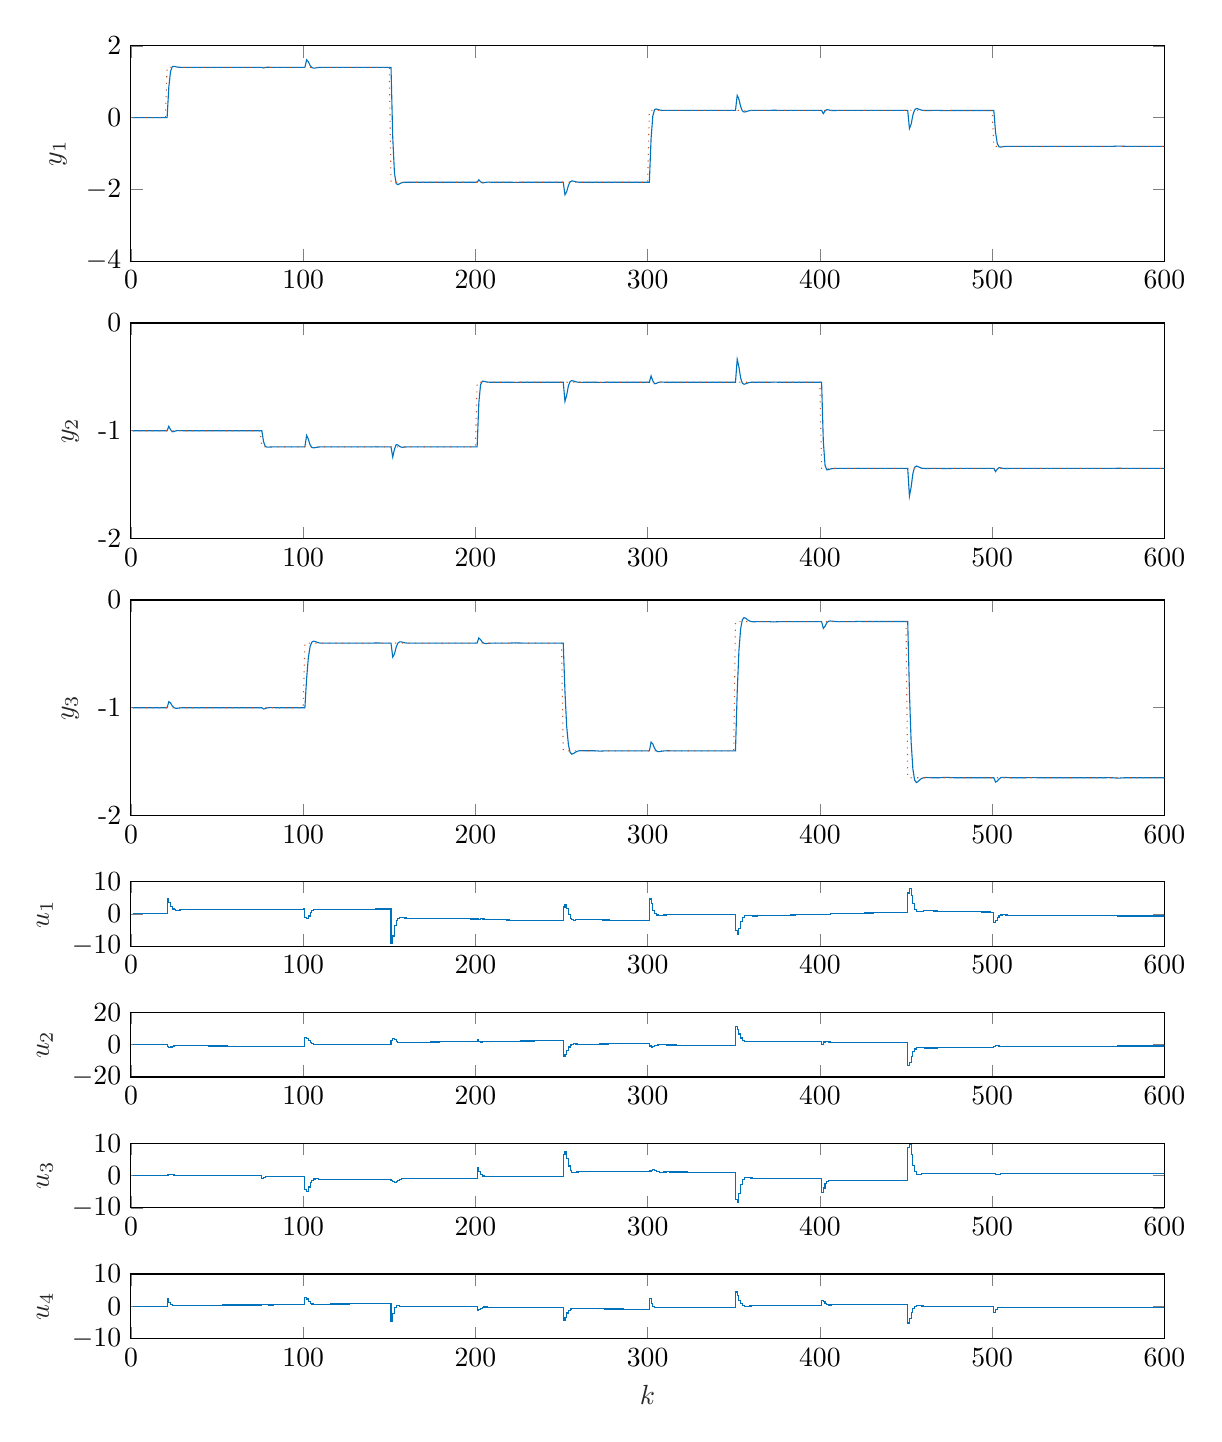
\begin{tikzpicture}

\begin{axis}[%
width=5.167in,
height=0.323in,
at={(0.646in,0.385in)},
scale only axis,
xmin=0,
xmax=600,
xtick={0,100,200,300,400,500,600},
xlabel style={font=\color{white!15!black}},
xlabel={$k$},
ymin=-10,
ymax=10,
ytick={-10,0,10},
ylabel style={font=\color{white!15!black}},
ylabel={$u_4$},
axis background/.style={fill=white}
]
\addplot[const plot, color=mycolor1, forget plot] table[row sep=crcr] {%
1	0\\
2	0\\
3	0\\
4	0\\
5	0\\
6	0\\
7	0\\
8	0\\
9	0\\
10	0\\
11	0\\
12	0\\
13	0\\
14	0\\
15	0\\
16	0\\
17	0\\
18	0\\
19	0\\
20	0\\
21	2.31539001573182\\
22	1.29014320630902\\
23	0.493417956912217\\
24	0.261649614943009\\
25	0.284024304877857\\
26	0.346618592917917\\
27	0.382365615726542\\
28	0.39206812746612\\
29	0.390334536850259\\
30	0.38679714692004\\
31	0.384795589039993\\
32	0.384436870120729\\
33	0.384971892010609\\
34	0.385785861280098\\
35	0.386575732359744\\
36	0.387252831443567\\
37	0.387825006563119\\
38	0.388325590378926\\
39	0.388783848560556\\
40	0.389218018493005\\
41	0.389637144311021\\
42	0.390044749457826\\
43	0.390441766889915\\
44	0.390828246984493\\
45	0.391204121550788\\
46	0.391569430850582\\
47	0.391924321299043\\
48	0.392268985639815\\
49	0.392603615886074\\
50	0.392928383514702\\
51	0.393243439472077\\
52	0.393548922960265\\
53	0.393844971298026\\
54	0.394131727320317\\
55	0.394409343603264\\
56	0.39467798410928\\
57	0.394937824157108\\
58	0.395189049474938\\
59	0.39543185483459\\
60	0.39566644254643\\
61	0.395893020954589\\
62	0.396111802998274\\
63	0.396323004869734\\
64	0.396526844785237\\
65	0.396723541877674\\
66	0.396913315214834\\
67	0.397096382943377\\
68	0.397272961555324\\
69	0.397443265270698\\
70	0.397607505528527\\
71	0.397765890577512\\
72	0.397918625156932\\
73	0.398065910258644\\
74	0.398207942961535\\
75	0.398344916330235\\
76	0.685370444461345\\
77	0.643343145771041\\
78	0.518831406863802\\
79	0.444524371652126\\
80	0.421714365892524\\
81	0.421276075687292\\
82	0.425625882771224\\
83	0.429297705574191\\
84	0.431779463942067\\
85	0.43353380859076\\
86	0.434899310085545\\
87	0.436036794199821\\
88	0.437027706915861\\
89	0.437922290341657\\
90	0.438751440899131\\
91	0.439530988528595\\
92	0.440267105892032\\
93	0.440961672374022\\
94	0.441615748974651\\
95	0.44223099193519\\
96	0.442809785880729\\
97	0.443354901559296\\
98	0.443869142065477\\
99	0.444355132069122\\
100	0.444815241801197\\
101	2.81974299050612\\
102	2.26823300328879\\
103	1.49292405572098\\
104	0.987294280966826\\
105	0.730832134343603\\
106	0.632907863948355\\
107	0.616549722044516\\
108	0.631830482813951\\
109	0.652884591600051\\
110	0.669844609841119\\
111	0.681125923919056\\
112	0.688233688738175\\
113	0.693084419791835\\
114	0.697027352993715\\
115	0.700741339749351\\
116	0.704445727137039\\
117	0.708135337951569\\
118	0.711737789731689\\
119	0.715188595904747\\
120	0.718452576785882\\
121	0.721520310609082\\
122	0.724397871170564\\
123	0.727098074797807\\
124	0.729635288192449\\
125	0.732023164707193\\
126	0.734274063505326\\
127	0.736399149108174\\
128	0.7384085711332\\
129	0.740311417370902\\
130	0.742115306996683\\
131	0.743825667267625\\
132	0.745445103692303\\
133	0.74697399956912\\
134	0.748414469587311\\
135	0.749780079267377\\
136	0.751110886792421\\
137	0.752485738303739\\
138	0.754022236017965\\
139	0.755894124185024\\
140	0.758434828126876\\
141	0.761843489361141\\
142	0.757915536674358\\
143	0.756352278353858\\
144	0.757380459553721\\
145	0.759173858020673\\
146	0.760764487204568\\
147	0.761924030873866\\
148	0.762737793283259\\
149	0.763362734689972\\
150	0.763919892838388\\
151	-4.52785181355668\\
152	-2.18387832527301\\
153	-0.362244029899981\\
154	0.16804497233945\\
155	0.117413706997658\\
156	-0.0251718535130171\\
157	-0.106415046963436\\
158	-0.128148809674417\\
159	-0.123761954168165\\
160	-0.115269757935531\\
161	-0.110304622598471\\
162	-0.109110316880323\\
163	-0.109973896386423\\
164	-0.111489430137724\\
165	-0.112963561983661\\
166	-0.114192936378648\\
167	-0.115194833560742\\
168	-0.116044804218478\\
169	-0.116809125272942\\
170	-0.117528888171023\\
171	-0.118224191768758\\
172	-0.118902534947283\\
173	-0.119565512642922\\
174	-0.120212718486604\\
175	-0.120843490399082\\
176	-0.12145742905244\\
177	-0.122054392084148\\
178	-0.12263435609878\\
179	-0.123197306276349\\
180	-0.123743186137812\\
181	-0.124271891537414\\
182	-0.124783289003827\\
183	-0.12527725404476\\
184	-0.125753744834318\\
185	-0.126212937698911\\
186	-0.126655430329208\\
187	-0.127082426445282\\
188	-0.127495609051147\\
189	-0.127896122816413\\
190	-0.128282019255926\\
191	-0.128644467365647\\
192	-0.128966105936974\\
193	-0.129229764318981\\
194	-0.129445871772498\\
195	-0.129683779551761\\
196	-0.130023322885065\\
197	-0.130273220688786\\
198	-0.130856910608537\\
199	-0.131350436316846\\
200	-0.131596849988108\\
201	-1.27926856692667\\
202	-1.1107191478595\\
203	-0.612277457402469\\
204	-0.314703738691796\\
205	-0.223150079391458\\
206	-0.221097201669249\\
207	-0.238199042242719\\
208	-0.252586086283217\\
209	-0.262209119830918\\
210	-0.268920800018068\\
211	-0.274080620923433\\
212	-0.278341330742401\\
213	-0.282042087553526\\
214	-0.285395237495796\\
215	-0.288516525684397\\
216	-0.291410858410232\\
217	-0.293959390992384\\
218	-0.29594381052371\\
219	-0.297175174302422\\
220	-0.297791039823274\\
221	-0.29863830204717\\
222	-0.304462038237197\\
223	-0.309345240351345\\
224	-0.312434644484775\\
225	-0.314131889973637\\
226	-0.314990122857818\\
227	-0.315574728741861\\
228	-0.316277326348667\\
229	-0.317236214698977\\
230	-0.318407090689916\\
231	-0.319678357591524\\
232	-0.320951005438124\\
233	-0.322167673054895\\
234	-0.323308806242561\\
235	-0.324377274234172\\
236	-0.325384371737713\\
237	-0.326341539315265\\
238	-0.327257231459036\\
239	-0.328136798820783\\
240	-0.32898350047805\\
241	-0.329799558451724\\
242	-0.33058685311003\\
243	-0.33134724794023\\
244	-0.3320826731372\\
245	-0.332795099609002\\
246	-0.333486488152782\\
247	-0.334158751796688\\
248	-0.334813739364709\\
249	-0.335453234531283\\
250	-0.336078960728871\\
251	-4.2941782503674\\
252	-3.37490724296556\\
253	-2.08266254975741\\
254	-1.23990654248156\\
255	-0.812452294402003\\
256	-0.649249454494333\\
257	-0.622011412310315\\
258	-0.647526142877206\\
259	-0.682684219335346\\
260	-0.711038527112688\\
261	-0.729945339680606\\
262	-0.741908064784585\\
263	-0.750082323647275\\
264	-0.756712089904499\\
265	-0.762954725076307\\
266	-0.769258246716813\\
267	-0.775783104032673\\
268	-0.782666107029726\\
269	-0.79018620208635\\
270	-0.799037319090852\\
271	-0.809650646053943\\
272	-0.803275747148574\\
273	-0.802101851557912\\
274	-0.8066650673814\\
275	-0.812808106087959\\
276	-0.818333427072299\\
277	-0.822732402259156\\
278	-0.826211925082397\\
279	-0.829141684267708\\
280	-0.831808443385186\\
281	-0.834356308517828\\
282	-0.836822944110673\\
283	-0.839197776221078\\
284	-0.841462805246576\\
285	-0.843609265243733\\
286	-0.845638774256591\\
287	-0.84755889800798\\
288	-0.849378868367118\\
289	-0.85110723119015\\
290	-0.85275114507264\\
291	-0.854316530314685\\
292	-0.855808451013333\\
293	-0.857231433935564\\
294	-0.858589653146973\\
295	-0.859887010106269\\
296	-0.86112715906085\\
297	-0.862313514148244\\
298	-0.863449255928476\\
299	-0.864537342143496\\
300	-0.865580521610236\\
301	2.44111867335501\\
302	0.975519522670317\\
303	-0.163582494623777\\
304	-0.495567527548883\\
305	-0.46445736034864\\
306	-0.375858778835186\\
307	-0.325583396165356\\
308	-0.31248609321194\\
309	-0.315699022184157\\
310	-0.321462192617595\\
311	-0.325003501389831\\
312	-0.326166541479372\\
313	-0.32601613131826\\
314	-0.325427521596112\\
315	-0.324842974647467\\
316	-0.324425639547839\\
317	-0.324234336129083\\
318	-0.324292620659511\\
319	-0.324517281879761\\
320	-0.324605894592085\\
321	-0.324227986862389\\
322	-0.32414540566399\\
323	-0.322664479562759\\
324	-0.321482100358029\\
325	-0.321227209512598\\
326	-0.321506009971226\\
327	-0.32184023773838\\
328	-0.322006813855099\\
329	-0.321989344960809\\
330	-0.321854920626751\\
331	-0.321673618514133\\
332	-0.321489462854638\\
333	-0.321320962769309\\
334	-0.321171173536404\\
335	-0.321036838172669\\
336	-0.320913766267846\\
337	-0.320799199901472\\
338	-0.320692628434379\\
339	-0.320595827549079\\
340	-0.320511793588653\\
341	-0.320441650463347\\
342	-0.320380805293605\\
343	-0.320323713652189\\
344	-0.32027254697359\\
345	-0.320228591249127\\
346	-0.320193994382137\\
347	-0.320171759407284\\
348	-0.320163746465398\\
349	-0.320169981569207\\
350	-0.320189442547299\\
351	4.42876170922999\\
352	3.32486943324257\\
353	1.77340779719707\\
354	0.761329539794537\\
355	0.247608150566719\\
356	0.0509808600395995\\
357	0.0175010658895582\\
358	0.0473115308574835\\
359	0.0886793379945696\\
360	0.121870310899081\\
361	0.143720949161826\\
362	0.157254931572863\\
363	0.166325877865322\\
364	0.173650007112908\\
365	0.180571015852588\\
366	0.187429435482857\\
367	0.193974935375458\\
368	0.199685645059246\\
369	0.20410991930431\\
370	0.207394959796042\\
371	0.210916898985844\\
372	0.222577300284451\\
373	0.232520888702103\\
374	0.239336261623896\\
375	0.243703755978925\\
376	0.246555225657674\\
377	0.248841908340344\\
378	0.251224698243778\\
379	0.253941785421747\\
380	0.256926614108906\\
381	0.260000054923971\\
382	0.263003471241365\\
383	0.265847062185864\\
384	0.268503311028104\\
385	0.270981367412736\\
386	0.273303878427763\\
387	0.275493595347527\\
388	0.277568614087379\\
389	0.279542281560499\\
390	0.281425338661094\\
391	0.283231559400552\\
392	0.28497974255542\\
393	0.286620635609468\\
394	0.288170211758167\\
395	0.289651916229569\\
396	0.291077193607236\\
397	0.292450311214933\\
398	0.293772671885278\\
399	0.295044998614187\\
400	0.296268678081906\\
401	1.82754446322772\\
402	1.60385391078591\\
403	0.940230874274136\\
404	0.544353048014453\\
405	0.423114791538128\\
406	0.421182831229464\\
407	0.44477948962432\\
408	0.464753809015158\\
409	0.478375710021865\\
410	0.488112478148002\\
411	0.495767324521528\\
412	0.502192232210848\\
413	0.507813393880813\\
414	0.512893762478628\\
415	0.517610137275216\\
416	0.522097426521442\\
417	0.52649501059698\\
418	0.530975254012813\\
419	0.535786826837166\\
420	0.541410111554082\\
421	0.548137921349754\\
422	0.544260166267076\\
423	0.543647062884346\\
424	0.546633060000541\\
425	0.550618683713577\\
426	0.554229388797086\\
427	0.557146336307765\\
428	0.559497929744062\\
429	0.561514296770236\\
430	0.563373708797829\\
431	0.565165276864946\\
432	0.566911616756417\\
433	0.568605239169766\\
434	0.570234056073716\\
435	0.571791802739947\\
436	0.573278822488448\\
437	0.574699450699061\\
438	0.576059552407109\\
439	0.577365126966532\\
440	0.578621297280269\\
441	0.579830871712974\\
442	0.580993962622848\\
443	0.582118082784795\\
444	0.583201949438321\\
445	0.584247136213876\\
446	0.585258239001822\\
447	0.586239715069481\\
448	0.587194614233579\\
449	0.588124814163797\\
450	0.589031696915448\\
451	-5.148437548763\\
452	-3.81375538739397\\
453	-1.93829292253972\\
454	-0.714616686162639\\
455	-0.0931517976361913\\
456	0.145128722980787\\
457	0.186244830210759\\
458	0.150858510084144\\
459	0.101481530119145\\
460	0.0619605110127825\\
461	0.0361191799557613\\
462	0.0203050962012895\\
463	0.00986294682944881\\
464	0.00151173151056829\\
465	-0.00637137148407208\\
466	-0.0141977726526759\\
467	-0.0216661422880547\\
468	-0.0281482015225372\\
469	-0.0331000876637615\\
470	-0.0366970618730686\\
471	-0.0405895551060842\\
472	-0.0542587975598558\\
473	-0.0658779467832164\\
474	-0.0737528506382496\\
475	-0.0786994470342029\\
476	-0.0818354829681262\\
477	-0.0843019480813143\\
478	-0.0868913899656883\\
479	-0.0898890617110482\\
480	-0.0932144575173421\\
481	-0.096651939134896\\
482	-0.100010500257018\\
483	-0.103181945394883\\
484	-0.106133312246668\\
485	-0.108876178226139\\
486	-0.111438531283584\\
487	-0.113847674422085\\
488	-0.116123026603241\\
489	-0.118275149835517\\
490	-0.120308778341394\\
491	-0.122229563816116\\
492	-0.124051630669016\\
493	-0.125790227322692\\
494	-0.127447482890044\\
495	-0.129026752573608\\
496	-0.130529659795509\\
497	-0.131956071554221\\
498	-0.13330741866769\\
499	-0.134587857914487\\
500	-0.135802980756668\\
501	-1.79080812320289\\
502	-1.05958828903385\\
503	-0.491545336595754\\
504	-0.326992479253212\\
505	-0.343921710185763\\
506	-0.389532376807326\\
507	-0.415921361306989\\
508	-0.423663903399083\\
509	-0.423196743582537\\
510	-0.421403214622248\\
511	-0.420673880080994\\
512	-0.421093270008958\\
513	-0.422136758349141\\
514	-0.423372490999918\\
515	-0.424574647013385\\
516	-0.425633703536138\\
517	-0.426463485613762\\
518	-0.426996960096734\\
519	-0.427311321493747\\
520	-0.427790074618598\\
521	-0.428866016982464\\
522	-0.429522004254994\\
523	-0.432017502159437\\
524	-0.434091866361352\\
525	-0.43490835062089\\
526	-0.434993734777754\\
527	-0.434987370424643\\
528	-0.435188375781775\\
529	-0.435620325441089\\
530	-0.436195517554133\\
531	-0.436822274230113\\
532	-0.437443598944099\\
533	-0.438036339779128\\
534	-0.438597624452078\\
535	-0.439132600666653\\
536	-0.439647481034686\\
537	-0.440147086139747\\
538	-0.440634806937943\\
539	-0.441113222612744\\
540	-0.441585019191589\\
541	-0.442055844316109\\
542	-0.442535032335289\\
543	-0.442989647043307\\
544	-0.443427672340593\\
545	-0.443861900440748\\
546	-0.444297774248214\\
547	-0.444736411124516\\
548	-0.445177293867534\\
549	-0.445619618937702\\
550	-0.446063110781048\\
551	-0.446508265645216\\
552	-0.446956114485454\\
553	-0.447407849020524\\
554	-0.447864589016592\\
555	-0.448327368128997\\
556	-0.44879726066934\\
557	-0.449275470733167\\
558	-0.449763092020531\\
559	-0.450260098635936\\
560	-0.450763059839688\\
561	-0.451261433476979\\
562	-0.451733725444844\\
563	-0.452148066209133\\
564	-0.452476841829654\\
565	-0.452738569278391\\
566	-0.453073863896974\\
567	-0.453829045059949\\
568	-0.455549344306536\\
569	-0.458701133367343\\
570	-0.462967507320792\\
571	-0.466324365270466\\
572	-0.457330717160223\\
573	-0.450312573201994\\
574	-0.447356817187764\\
575	-0.447515170058764\\
576	-0.449470760862215\\
577	-0.451875017693645\\
578	-0.453797550279035\\
579	-0.454918707610732\\
580	-0.455358901545804\\
581	-0.455400092639727\\
582	-0.455292817392511\\
583	-0.45518594925733\\
584	-0.455135929373815\\
585	-0.455143947463882\\
586	-0.455190034953766\\
587	-0.455253826751046\\
588	-0.455323359911066\\
589	-0.455396345358487\\
590	-0.455476611227058\\
591	-0.455566078591281\\
592	-0.455655763726791\\
593	-0.455734664201554\\
594	-0.455806915948702\\
595	-0.455874639631738\\
596	-0.455941545820767\\
597	-0.456013015139495\\
598	-0.456092159917133\\
599	-0.456178471728523\\
600	-0.456269409966281\\
};
\end{axis}

\begin{axis}[%
width=5.167in,
height=0.323in,
at={(0.646in,1.039in)},
scale only axis,
xmin=0,
xmax=600,
xtick={0,100,200,300,400,500,600},
ymin=-10,
ymax=10,
ytick={-10,0,10},
ylabel style={font=\color{white!15!black}},
ylabel={$u_3$},
axis background/.style={fill=white}
]
\addplot[const plot, color=mycolor1, forget plot] table[row sep=crcr] {%
1	0\\
2	0\\
3	0\\
4	0\\
5	0\\
6	0\\
7	0\\
8	0\\
9	0\\
10	0\\
11	0\\
12	0\\
13	0\\
14	0\\
15	0\\
16	0\\
17	0\\
18	0\\
19	0\\
20	0\\
21	0.166001048542126\\
22	0.314148897426233\\
23	0.413730560246662\\
24	0.302847224796797\\
25	0.116753790618091\\
26	-0.015258407302264\\
27	-0.0685449627801358\\
28	-0.0729199548028004\\
29	-0.060693672114897\\
30	-0.0492542252830567\\
31	-0.0435547432009891\\
32	-0.0427300383904135\\
33	-0.0445772794858774\\
34	-0.047390839236921\\
35	-0.0502761340165552\\
36	-0.0529162592228893\\
37	-0.0552815895277656\\
38	-0.0574371139209696\\
39	-0.0594511888742896\\
40	-0.0613677819127404\\
41	-0.0632075397659771\\
42	-0.0649769474781112\\
43	-0.0666764943426273\\
44	-0.0683054969706754\\
45	-0.069864095020055\\
46	-0.0713536157330498\\
47	-0.0727762769434486\\
48	-0.0741347751720629\\
49	-0.0754319746717073\\
50	-0.0766707311899142\\
51	-0.0778538146385748\\
52	-0.0789838857120455\\
53	-0.080063494560323\\
54	-0.0810950849044203\\
55	-0.0820809974474708\\
56	-0.0830234716572464\\
57	-0.083924646747346\\
58	-0.0847865627720802\\
59	-0.0856111623296322\\
60	-0.0864002929743545\\
61	-0.0871557102175932\\
62	-0.0878790809267394\\
63	-0.0885719869461647\\
64	-0.0892359288069496\\
65	-0.0898723294364246\\
66	-0.0904825378114642\\
67	-0.0910678325211046\\
68	-0.0916294252163146\\
69	-0.0921684639342336\\
70	-0.0926860362871576\\
71	-0.0931831725121609\\
72	-0.093660848378722\\
73	-0.0941199879543355\\
74	-0.0945614662293132\\
75	-0.094986111604037\\
76	-0.931468789497236\\
77	-0.668756269387234\\
78	-0.41427707530709\\
79	-0.290250187652387\\
80	-0.243604526266678\\
81	-0.23101996784464\\
82	-0.23102432507973\\
83	-0.234411511182175\\
84	-0.23774251491452\\
85	-0.240078825843605\\
86	-0.241448067352814\\
87	-0.242159950173361\\
88	-0.242522294640582\\
89	-0.24274664444238\\
90	-0.242943690955228\\
91	-0.243153532232781\\
92	-0.243379597364687\\
93	-0.243612686900009\\
94	-0.243843284248401\\
95	-0.244065571973654\\
96	-0.244277304408941\\
97	-0.244478415796515\\
98	-0.244669751739057\\
99	-0.244852313290222\\
100	-0.24502694288079\\
101	-4.42578720943074\\
102	-4.85768953640604\\
103	-3.54631378509432\\
104	-2.21295558637585\\
105	-1.4086828211134\\
106	-1.07261915172789\\
107	-1.00328548951281\\
108	-1.04120366820142\\
109	-1.09906308648692\\
110	-1.14279401068628\\
111	-1.16679751755044\\
112	-1.17629242855369\\
113	-1.17800316571682\\
114	-1.17672030833445\\
115	-1.17492352234417\\
116	-1.17349769737913\\
117	-1.17253090056252\\
118	-1.17184797176908\\
119	-1.17126810088853\\
120	-1.1706835298641\\
121	-1.17005483721498\\
122	-1.1693827591172\\
123	-1.16868354216382\\
124	-1.1679747659041\\
125	-1.16726986429136\\
126	-1.16657754025476\\
127	-1.16590298945295\\
128	-1.16524909337877\\
129	-1.16461664844701\\
130	-1.16400323350783\\
131	-1.1634008759699\\
132	-1.16279383255729\\
133	-1.16216005925459\\
134	-1.16148326946503\\
135	-1.16078551678612\\
136	-1.16018885652886\\
137	-1.1599968542884\\
138	-1.1607182522952\\
139	-1.16278198705855\\
140	-1.16556283424506\\
141	-1.16649053011917\\
142	-1.16053083739194\\
143	-1.15417841442361\\
144	-1.1524295535263\\
145	-1.15400482831788\\
146	-1.15606284370812\\
147	-1.15716829354444\\
148	-1.15728837650685\\
149	-1.15690563613028\\
150	-1.15643188791573\\
151	-1.53548541124688\\
152	-1.87385286638033\\
153	-2.10129327950361\\
154	-1.84770881322876\\
155	-1.42222776594537\\
156	-1.12036407168002\\
157	-0.99844778473958\\
158	-0.98833521186774\\
159	-1.01617661058608\\
160	-1.04222877458352\\
161	-1.05517025823248\\
162	-1.05697807925967\\
163	-1.05268657291598\\
164	-1.04619365100143\\
165	-1.03954350989622\\
166	-1.0334600217089\\
167	-1.0280104731645\\
168	-1.0230459162354\\
169	-1.01840971732814\\
170	-1.01400099459617\\
171	-1.00977217537624\\
172	-1.00570806163951\\
173	-1.0018071654238\\
174	-0.99807068433207\\
175	-0.994497938810587\\
176	-0.991085537777762\\
177	-0.987828057608664\\
178	-0.984718987455174\\
179	-0.981751450717159\\
180	-0.978918627782938\\
181	-0.976213958614815\\
182	-0.973631210366045\\
183	-0.97116443953573\\
184	-0.968807810813927\\
185	-0.966555196932083\\
186	-0.964399539168227\\
187	-0.962332202620374\\
188	-0.960343132196501\\
189	-0.958423482782593\\
190	-0.956573041011953\\
191	-0.954813649530256\\
192	-0.953204347216453\\
193	-0.951842138849646\\
194	-0.950819063914787\\
195	-0.950113008225245\\
196	-0.949455494370268\\
197	-0.947040181216801\\
198	-0.944202660005203\\
199	-0.942112634240244\\
200	-0.94092404965916\\
201	2.4040912292383\\
202	1.35233740792269\\
203	0.333709735042826\\
204	-0.162915873408581\\
205	-0.349890680576329\\
206	-0.400558532081041\\
207	-0.400846374100566\\
208	-0.387594756345206\\
209	-0.374562364159917\\
210	-0.365497067650881\\
211	-0.360272587688113\\
212	-0.35762085307332\\
213	-0.356268172632083\\
214	-0.355330599970172\\
215	-0.354387025823788\\
216	-0.353465672939706\\
217	-0.353052310464791\\
218	-0.354073910132728\\
219	-0.357630028425692\\
220	-0.364134421061779\\
221	-0.371731933844757\\
222	-0.36149531472256\\
223	-0.347148346361168\\
224	-0.338895970186202\\
225	-0.337658637511821\\
226	-0.340280983531047\\
227	-0.343657512722082\\
228	-0.346109568609037\\
229	-0.347239464276479\\
230	-0.34733812295811\\
231	-0.346876380228328\\
232	-0.346232014504989\\
233	-0.345614992361\\
234	-0.345098422159298\\
235	-0.344678874344922\\
236	-0.344325930580241\\
237	-0.344009904684574\\
238	-0.343711646403017\\
239	-0.343422364613581\\
240	-0.343139939509949\\
241	-0.342865299620621\\
242	-0.342600107793526\\
243	-0.342345724960482\\
244	-0.342102983792029\\
245	-0.341872320306896\\
246	-0.341653979125818\\
247	-0.341448167520004\\
248	-0.341255133012053\\
249	-0.341075183997776\\
250	-0.340908685193979\\
251	6.6268988485298\\
252	7.34660686365361\\
253	5.16084724158029\\
254	2.9384447118866\\
255	1.59784430891064\\
256	1.03758417510651\\
257	0.921865257515066\\
258	0.984891488950327\\
259	1.08114766601445\\
260	1.15385285798296\\
261	1.19366944070305\\
262	1.20926462694394\\
263	1.21174156047196\\
264	1.20904152147489\\
265	1.20537548302141\\
266	1.20251909620311\\
267	1.20131856075894\\
268	1.2026413762616\\
269	1.20716241280337\\
270	1.21327160952863\\
271	1.21502991046483\\
272	1.20093486696979\\
273	1.18586198807922\\
274	1.18126376101681\\
275	1.18424055975986\\
276	1.18831390044681\\
277	1.19021273383604\\
278	1.18986776151998\\
279	1.18838545356397\\
280	1.18670947693629\\
281	1.18526968514955\\
282	1.18412433338618\\
283	1.18318316550377\\
284	1.1823474804317\\
285	1.18155863923597\\
286	1.18079580726337\\
287	1.18005877146637\\
288	1.17935356118952\\
289	1.17868513147007\\
290	1.17805539639693\\
291	1.17746381097997\\
292	1.1769085513843\\
293	1.17638742225129\\
294	1.1758983180017\\
295	1.17543935792792\\
296	1.17500886162998\\
297	1.17460528099898\\
298	1.17422714319502\\
299	1.17387301781766\\
300	1.17354150333146\\
301	1.41037558036779\\
302	1.62172498359751\\
303	1.763712737406\\
304	1.60505365248473\\
305	1.33896803594435\\
306	1.15015711479437\\
307	1.07382684923362\\
308	1.06738552383206\\
309	1.08467485078992\\
310	1.10085178956716\\
311	1.10883289345825\\
312	1.10983947736101\\
313	1.10699749699584\\
314	1.10272707407784\\
315	1.09832390263967\\
316	1.0943461385023\\
317	1.0910890829128\\
318	1.08885821696122\\
319	1.08793565148346\\
320	1.08818515584223\\
321	1.08851946388032\\
322	1.08171858678886\\
323	1.07313660681853\\
324	1.06746416226218\\
325	1.06532701394051\\
326	1.06500606008736\\
327	1.06482773239701\\
328	1.06406203633674\\
329	1.06270322250848\\
330	1.06101240588586\\
331	1.05923465606661\\
332	1.05751216617118\\
333	1.05589788483215\\
334	1.05439418200027\\
335	1.05298374815338\\
336	1.05164657587945\\
337	1.05036711568754\\
338	1.04913702251967\\
339	1.04795663206044\\
340	1.04683506932928\\
341	1.04578619753161\\
342	1.04481552983806\\
343	1.04386140719262\\
344	1.04290005856401\\
345	1.04194580324962\\
346	1.04102054298797\\
347	1.04013695324739\\
348	1.03929594605083\\
349	1.03849083775864\\
350	1.03771274003847\\
351	-7.32423163347144\\
352	-8.1884588519807\\
353	-5.56613021302602\\
354	-2.89983726661435\\
355	-1.29171540988324\\
356	-0.620011088019084\\
357	-0.481764629733574\\
358	-0.558017989906453\\
359	-0.674150073381749\\
360	-0.762028308336087\\
361	-0.810476862055161\\
362	-0.82997946938884\\
363	-0.834054957271448\\
364	-0.832348063538826\\
365	-0.829783313601465\\
366	-0.827817616794979\\
367	-0.825796089032563\\
368	-0.821886139530425\\
369	-0.813958252977816\\
370	-0.80114729554714\\
371	-0.786482479438921\\
372	-0.801512271394409\\
373	-0.823391631323085\\
374	-0.83514172107036\\
375	-0.835250278404938\\
376	-0.828989512532503\\
377	-0.821542070312275\\
378	-0.815708572122702\\
379	-0.812152578249886\\
380	-0.810388952247929\\
381	-0.809632219799412\\
382	-0.809251657103858\\
383	-0.808895695684162\\
384	-0.808439722910359\\
385	-0.807885352251039\\
386	-0.80727811738575\\
387	-0.806662518977542\\
388	-0.806068591332544\\
389	-0.805516838276279\\
390	-0.80502871860506\\
391	-0.804629222406522\\
392	-0.80432484723178\\
393	-0.803986711376617\\
394	-0.803595799540224\\
395	-0.803209839259273\\
396	-0.802872793946788\\
397	-0.802591075652266\\
398	-0.80235028703714\\
399	-0.802133926372718\\
400	-0.801931740641604\\
401	-5.26080176305083\\
402	-3.85738937999357\\
403	-2.49797710559588\\
404	-1.83439622548905\\
405	-1.58359715954777\\
406	-1.5145352981399\\
407	-1.51268864952177\\
408	-1.52895463852805\\
409	-1.54498756392193\\
410	-1.5557743746259\\
411	-1.56144758007471\\
412	-1.56363360956832\\
413	-1.56394025796087\\
414	-1.56347045599294\\
415	-1.56284436342511\\
416	-1.56244879077384\\
417	-1.5627345253001\\
418	-1.5643783157443\\
419	-1.56794138177251\\
420	-1.57249887097926\\
421	-1.57436647412689\\
422	-1.56635165017073\\
423	-1.55773666001393\\
424	-1.55566415001048\\
425	-1.55831067876689\\
426	-1.561620324356\\
427	-1.56354499486845\\
428	-1.56403963344546\\
429	-1.56379509384548\\
430	-1.56340103238476\\
431	-1.56312627612803\\
432	-1.56300756129676\\
433	-1.56298882187537\\
434	-1.56300856837827\\
435	-1.56303008327822\\
436	-1.56304008229677\\
437	-1.56303841033459\\
438	-1.56302984962803\\
439	-1.56302032756395\\
440	-1.56301582183943\\
441	-1.56302186830938\\
442	-1.56304124293969\\
443	-1.56305327865463\\
444	-1.56304530694956\\
445	-1.56302113272881\\
446	-1.56299157525883\\
447	-1.5629638987985\\
448	-1.56293873882043\\
449	-1.56291253635703\\
450	-1.56288092313908\\
451	8.54025895550417\\
452	9.58368579081214\\
453	6.41421747425719\\
454	3.19165124912151\\
455	1.24773357322643\\
456	0.435345027450249\\
457	0.267575253340544\\
458	0.3590156754363\\
459	0.498664765936567\\
460	0.604194563653189\\
461	0.662099729323432\\
462	0.685046733801535\\
463	0.689369323196134\\
464	0.686720316288818\\
465	0.683049882844512\\
466	0.680120498711729\\
467	0.677147195463023\\
468	0.671927361676733\\
469	0.661902000248963\\
470	0.646030635554523\\
471	0.627947207733546\\
472	0.645509493130969\\
473	0.671303371682143\\
474	0.684954233647255\\
475	0.684647333179231\\
476	0.67670924753483\\
477	0.667359037704721\\
478	0.659957266609394\\
479	0.655299893692618\\
480	0.652804233800954\\
481	0.651526988077905\\
482	0.650710587783514\\
483	0.649933162780138\\
484	0.649047253010112\\
485	0.648059761697215\\
486	0.6470328504131\\
487	0.646027014788233\\
488	0.645077908557765\\
489	0.644191829574513\\
490	0.643350219872793\\
491	0.642521803532997\\
492	0.641688087477896\\
493	0.640943161288088\\
494	0.640319056755378\\
495	0.639785255423156\\
496	0.639299223267596\\
497	0.638834169294689\\
498	0.638383124388853\\
499	0.637951927962297\\
500	0.637550220347422\\
501	0.518613104523209\\
502	0.412467843869109\\
503	0.341051349117616\\
504	0.420002724812387\\
505	0.552707932167762\\
506	0.646812834998761\\
507	0.684711427742077\\
508	0.687696993226247\\
509	0.678846851680734\\
510	0.670582565472485\\
511	0.666449836813523\\
512	0.665848152759179\\
513	0.667230397770787\\
514	0.669398860665333\\
515	0.671690123402961\\
516	0.673737067792724\\
517	0.67518066027936\\
518	0.675528056825647\\
519	0.674316251372365\\
520	0.671674512978852\\
521	0.669030235758989\\
522	0.676003464749593\\
523	0.685453784801683\\
524	0.691125418909195\\
525	0.692181222417476\\
526	0.690909537742788\\
527	0.68953747290338\\
528	0.689033864424426\\
529	0.68940192161599\\
530	0.690289182457594\\
531	0.69136474780508\\
532	0.692434906756059\\
533	0.693424542003402\\
534	0.694324891261832\\
535	0.695151690678647\\
536	0.695922641338944\\
537	0.696649846589507\\
538	0.697340863565635\\
539	0.698003559467755\\
540	0.698650988300012\\
541	0.699300710606888\\
542	0.699959361749405\\
543	0.700548758335969\\
544	0.701058931058215\\
545	0.701527471708916\\
546	0.701983099618057\\
547	0.702430908348526\\
548	0.702862893992993\\
549	0.703269667261827\\
550	0.703645669689268\\
551	0.703989332219689\\
552	0.7043012844243\\
553	0.704582700914529\\
554	0.704834585326146\\
555	0.705057963426089\\
556	0.705254575143692\\
557	0.705427435737858\\
558	0.705580300014431\\
559	0.70571456560647\\
560	0.705821909205098\\
561	0.705872098120391\\
562	0.705799942452354\\
563	0.705505548477557\\
564	0.704898258016932\\
565	0.704030007055756\\
566	0.703355896650227\\
567	0.70408236448195\\
568	0.708360200278652\\
569	0.718754376550515\\
570	0.736208381607324\\
571	0.75621709369521\\
572	0.733038932028282\\
573	0.699847824568537\\
574	0.681315367626086\\
575	0.679674140560022\\
576	0.687304768002367\\
577	0.69670675823066\\
578	0.703826796039503\\
579	0.707706709279648\\
580	0.709052223333705\\
581	0.709003704638546\\
582	0.708476361025789\\
583	0.707979188415552\\
584	0.707689127104367\\
585	0.707596210565236\\
586	0.707623406213151\\
587	0.707695470930752\\
588	0.707766998738004\\
589	0.707827893735788\\
590	0.707897954040861\\
591	0.708012279867659\\
592	0.708190658842297\\
593	0.70831780697113\\
594	0.708352946315052\\
595	0.708330407147858\\
596	0.708298995763184\\
597	0.708288690515096\\
598	0.708305750955891\\
599	0.708341136316033\\
600	0.708381316985432\\
};
\end{axis}

\begin{axis}[%
width=5.167in,
height=0.323in,
at={(0.646in,1.693in)},
scale only axis,
xmin=0,
xmax=600,
xtick={0,100,200,300,400,500,600},
ymin=-20,
ymax=20,
ytick={-20,0,20},
ylabel style={font=\color{white!15!black}},
ylabel={$u_2$},
axis background/.style={fill=white}
]
\addplot[const plot, color=mycolor1, forget plot] table[row sep=crcr] {%
1	0\\
2	0\\
3	0\\
4	0\\
5	0\\
6	0\\
7	0\\
8	0\\
9	0\\
10	0\\
11	0\\
12	0\\
13	0\\
14	0\\
15	0\\
16	0\\
17	0\\
18	0\\
19	0\\
20	0\\
21	-1.03439798946634\\
22	-1.69727194828909\\
23	-1.3852060732059\\
24	-0.925598035768924\\
25	-0.65212436072567\\
26	-0.550795839188215\\
27	-0.539998725000089\\
28	-0.562737249553766\\
29	-0.591258386257487\\
30	-0.615394029921105\\
31	-0.633420625965232\\
32	-0.646776465390228\\
33	-0.657422406975803\\
34	-0.666818353183239\\
35	-0.675760087697641\\
36	-0.684557543676177\\
37	-0.69326347021925\\
38	-0.701837258098032\\
39	-0.710229206634409\\
40	-0.718409247974676\\
41	-0.726367983288515\\
42	-0.734108892130393\\
43	-0.741640799731093\\
44	-0.748973289881896\\
45	-0.756114782796396\\
46	-0.763072191473237\\
47	-0.769851228084465\\
48	-0.776456826388658\\
49	-0.782893466465638\\
50	-0.789165366775786\\
51	-0.795276577542266\\
52	-0.801231019096756\\
53	-0.807032496488679\\
54	-0.812684706932525\\
55	-0.818191246486995\\
56	-0.82355561721123\\
57	-0.828781234252555\\
58	-0.833871432158873\\
59	-0.838829470061271\\
60	-0.843658535718798\\
61	-0.848361748608288\\
62	-0.852942162295148\\
63	-0.857402766296504\\
64	-0.86174648759809\\
65	-0.865976191937186\\
66	-0.870094684926887\\
67	-0.874104713072735\\
68	-0.878008964716641\\
69	-0.881810070932677\\
70	-0.885510606393783\\
71	-0.889113090222315\\
72	-0.892619986834137\\
73	-0.896033706783543\\
74	-0.89935660761339\\
75	-0.902590994713396\\
76	-1.20834697380044\\
77	-0.922968245103808\\
78	-0.847570529951245\\
79	-0.884661505708378\\
80	-0.928211967607994\\
81	-0.952544985869544\\
82	-0.96231123152195\\
83	-0.965446286776214\\
84	-0.966860826530274\\
85	-0.968624781171501\\
86	-0.971192530562475\\
87	-0.974367194398715\\
88	-0.977831815876193\\
89	-0.981353804585746\\
90	-0.984813967778574\\
91	-0.988172230218421\\
92	-0.991427652498662\\
93	-0.994591861072075\\
94	-0.997676408307165\\
95	-1.00068899120871\\
96	-1.00363373227532\\
97	-1.0065125865519\\
98	-1.00932657390701\\
99	-1.0120765046693\\
100	-1.01476328260865\\
101	4.69690939496031\\
102	4.02800434052687\\
103	2.49148012582669\\
104	1.27229916111053\\
105	0.54241974517053\\
106	0.215903532785561\\
107	0.133983265048694\\
108	0.158253060955651\\
109	0.205369826431941\\
110	0.240418319110483\\
111	0.256741337991954\\
112	0.25897246905772\\
113	0.253563677024739\\
114	0.24519412114913\\
115	0.236315994471875\\
116	0.227827326574965\\
117	0.219842701393988\\
118	0.212211877170402\\
119	0.204771802503387\\
120	0.197425294323924\\
121	0.19013841599362\\
122	0.182914474430622\\
123	0.175770870165661\\
124	0.168725714620048\\
125	0.161792680843282\\
126	0.154980518389304\\
127	0.148294299119382\\
128	0.141736624517597\\
129	0.135307882254593\\
130	0.129005149617757\\
131	0.122819878835636\\
132	0.116735636951979\\
133	0.110729447729758\\
134	0.104783574489471\\
135	0.0989166007725979\\
136	0.0932372896780456\\
137	0.088007392702112\\
138	0.0836965169017235\\
139	0.0811034149480908\\
140	0.0816356170235068\\
141	0.0859754274359501\\
142	0.0655543899971211\\
143	0.0512792925410368\\
144	0.0465114085468693\\
145	0.045408365507769\\
146	0.0439760566990619\\
147	0.0411216621129164\\
148	0.0372043300944861\\
149	0.0328696901289009\\
150	0.0285565976381958\\
151	2.38877703009299\\
152	3.90000603075759\\
153	3.18296117162435\\
154	2.12879182108714\\
155	1.50016077382373\\
156	1.26508274303879\\
157	1.23701079901439\\
158	1.285670297252\\
159	1.34762672172896\\
160	1.3996384223846\\
161	1.43776457619561\\
162	1.46529091870309\\
163	1.48669748435013\\
164	1.50531931432377\\
165	1.52297356956884\\
166	1.54036698978685\\
167	1.55761852995365\\
168	1.57463379424789\\
169	1.59129763194181\\
170	1.6075397874513\\
171	1.62333726808838\\
172	1.63869653778532\\
173	1.65363630024138\\
174	1.66817701407346\\
175	1.68233649860245\\
176	1.69612914749871\\
177	1.70956662941072\\
178	1.72265885739035\\
179	1.73541474185944\\
180	1.74784264941536\\
181	1.75995064190293\\
182	1.77174657813412\\
183	1.78323810752038\\
184	1.79443252086933\\
185	1.80533638814381\\
186	1.81595496138547\\
187	1.82629153839055\\
188	1.83634746432949\\
189	1.84612421697866\\
190	1.85562984800908\\
191	1.8648921573907\\
192	1.87397860296538\\
193	1.88301489773031\\
194	1.89217585990576\\
195	1.90158925612786\\
196	1.91105110580284\\
197	1.91737836130879\\
198	1.92297827162683\\
199	1.92960133594462\\
200	1.937080098998\\
201	3.15515230112615\\
202	2.00875126619647\\
203	1.70221158557049\\
204	1.84559355280365\\
205	2.01484864614916\\
206	2.10732405197392\\
207	2.14165278944331\\
208	2.14958807205149\\
209	2.15077149335022\\
210	2.15347344188392\\
211	2.15949266709777\\
212	2.16800947064812\\
213	2.17771017813093\\
214	2.18762086192259\\
215	2.19727434541194\\
216	2.20667736280739\\
217	2.21630615589231\\
218	2.22714138867025\\
219	2.24054080926306\\
220	2.25747032822963\\
221	2.27625010123951\\
222	2.27282880709748\\
223	2.26726674559404\\
224	2.26785095385177\\
225	2.27476953058531\\
226	2.28522904018391\\
227	2.29637234224263\\
228	2.30653767119434\\
229	2.315277704073\\
230	2.32284296512084\\
231	2.32968249856518\\
232	2.33616582496014\\
233	2.34250312909055\\
234	2.34877210748833\\
235	2.35497525563811\\
236	2.36108771793048\\
237	2.3670844445845\\
238	2.37295007827018\\
239	2.37867907373422\\
240	2.38427227960764\\
241	2.38973348137287\\
242	2.39506715948382\\
243	2.40027746802114\\
244	2.40536799875049\\
245	2.41034189851159\\
246	2.41520206406158\\
247	2.41995129103503\\
248	2.42459235030927\\
249	2.4291280091185\\
250	2.43356102696646\\
251	-7.08593477840452\\
252	-5.97112994523271\\
253	-3.41028795756291\\
254	-1.37834523026264\\
255	-0.161897830197549\\
256	0.382285821006956\\
257	0.518818061291096\\
258	0.47837404484777\\
259	0.399856308473879\\
260	0.341455737620871\\
261	0.314272872155275\\
262	0.310607491684523\\
263	0.319823731331527\\
264	0.33415798135106\\
265	0.349452233768255\\
266	0.363940517122278\\
267	0.376825146626929\\
268	0.387282433967647\\
269	0.393759471172581\\
270	0.393200054853018\\
271	0.384097425215112\\
272	0.431739827065251\\
273	0.465448087696115\\
274	0.477503351837311\\
275	0.481231743745536\\
276	0.485743735802836\\
277	0.493525052011805\\
278	0.503746872868025\\
279	0.514927966880442\\
280	0.526061068816945\\
281	0.536745768172508\\
282	0.546953966021832\\
283	0.556789240016968\\
284	0.566353305815473\\
285	0.575705020769438\\
286	0.584865926835059\\
287	0.593837850199884\\
288	0.602616809313043\\
289	0.611199940979944\\
290	0.619587334429612\\
291	0.627781466525212\\
292	0.635786073751449\\
293	0.643605280760235\\
294	0.651243151815446\\
295	0.658703554486748\\
296	0.665990178258021\\
297	0.673106596782349\\
298	0.680056320806427\\
299	0.686842828381248\\
300	0.693469576709844\\
301	-0.777771410903072\\
302	-1.7184166983358\\
303	-1.26644035595598\\
304	-0.603835808869005\\
305	-0.207280748996396\\
306	-0.0567878298710588\\
307	-0.0357635674597014\\
308	-0.0627831804809322\\
309	-0.0981966974144643\\
310	-0.127473389494129\\
311	-0.148141671151024\\
312	-0.162239914876485\\
313	-0.172546290805003\\
314	-0.181125146038458\\
315	-0.189119376547673\\
316	-0.197056425650263\\
317	-0.205253485736681\\
318	-0.21413186121647\\
319	-0.224290163029306\\
320	-0.236170968828503\\
321	-0.248923613260548\\
322	-0.249800033420086\\
323	-0.248419801530938\\
324	-0.25177579882234\\
325	-0.25918761428019\\
326	-0.267868648837678\\
327	-0.276075531066734\\
328	-0.283316399423113\\
329	-0.289729657447326\\
330	-0.29560685887488\\
331	-0.301183528164347\\
332	-0.306593909917949\\
333	-0.311892440459467\\
334	-0.317088454742878\\
335	-0.322172946072243\\
336	-0.327133655089544\\
337	-0.331961904364926\\
338	-0.336655823578725\\
339	-0.341222626191439\\
340	-0.34567860354757\\
341	-0.350041248674586\\
342	-0.354310758785042\\
343	-0.358444679824694\\
344	-0.362432215481732\\
345	-0.366284150888399\\
346	-0.370020657315363\\
347	-0.373659165114732\\
348	-0.377207508583635\\
349	-0.380665051985703\\
350	-0.384027677335789\\
351	11.0413027198489\\
352	9.70545503176809\\
353	6.63434752296345\\
354	4.19790480301207\\
355	2.740042573365\\
356	2.08888272703086\\
357	1.9268887308419\\
358	1.9772466073651\\
359	2.07326976479873\\
360	2.14513402244341\\
361	2.17954622310225\\
362	2.18581876218674\\
363	2.17692552085597\\
364	2.16229240120742\\
365	2.14680358932495\\
366	2.13197291748535\\
367	2.11722586177553\\
368	2.10070137697232\\
369	2.07988389186722\\
370	2.05301702052965\\
371	2.02285674515985\\
372	2.0295049969874\\
373	2.03956636876141\\
374	2.03926755424283\\
375	2.02832501464749\\
376	2.01141519701556\\
377	1.99331366941773\\
378	1.97679919344599\\
379	1.96262385662979\\
380	1.95037522897159\\
381	1.93930916455352\\
382	1.92881340599665\\
383	1.91854048306806\\
384	1.90836232663917\\
385	1.89827461052185\\
386	1.88831725595449\\
387	1.87853060220207\\
388	1.8689419803464\\
389	1.85956922298828\\
390	1.8504291640731\\
391	1.84154587347592\\
392	1.83294225318444\\
393	1.82445736956292\\
394	1.81609104535838\\
395	1.80789541399582\\
396	1.79990420949035\\
397	1.79212276286943\\
398	1.78453832538539\\
399	1.77713374109832\\
400	1.76989618037725\\
401	0.148910461472501\\
402	1.68035262686507\\
403	2.09161555348281\\
404	1.90266768885751\\
405	1.67900654214723\\
406	1.55758357526176\\
407	1.51360291369066\\
408	1.50474897901679\\
409	1.50483781409076\\
410	1.50283242321988\\
411	1.49630461058812\\
412	1.48628862823114\\
413	1.4744499944755\\
414	1.46201189567089\\
415	1.44964470201067\\
416	1.43772569136214\\
417	1.42664197114844\\
418	1.41701053191292\\
419	1.40991890413069\\
420	1.40734477809651\\
421	1.4102487715057\\
422	1.37781615046024\\
423	1.35420168462915\\
424	1.34421040278969\\
425	1.33949864293175\\
426	1.33436217253623\\
427	1.32724070454268\\
428	1.31864774065173\\
429	1.30950581796406\\
430	1.30044198705821\\
431	1.29170447579554\\
432	1.28330910707859\\
433	1.27518953043024\\
434	1.26728049059066\\
435	1.25954329286063\\
436	1.2519624016872\\
437	1.24453498222112\\
438	1.23726331550676\\
439	1.2301515128534\\
440	1.22320325965921\\
441	1.21641679526895\\
442	1.20978129191664\\
443	1.20330121272085\\
444	1.1969542946534\\
445	1.19073268952225\\
446	1.18464336478872\\
447	1.17869311519476\\
448	1.17288189872946\\
449	1.16720444263969\\
450	1.16165402517107\\
451	-12.6533270534005\\
452	-11.0483142807556\\
453	-7.3462968892297\\
454	-4.41093944232803\\
455	-2.65781269657396\\
456	-1.8792363759759\\
457	-1.6915259187481\\
458	-1.76020285106209\\
459	-1.88385903203661\\
460	-1.97812817472412\\
461	-2.02695205131366\\
462	-2.0415871812269\\
463	-2.037714169176\\
464	-2.02672648588691\\
465	-2.01453037906832\\
466	-2.00296170513562\\
467	-1.99133712889167\\
468	-1.9774249454417\\
469	-1.95820769211961\\
470	-1.93157994694377\\
471	-1.90085212758729\\
472	-1.91415036084796\\
473	-1.93140414744053\\
474	-1.93608946145471\\
475	-1.92786986264263\\
476	-1.91236074722726\\
477	-1.89529631418432\\
478	-1.8800144288405\\
479	-1.86742071566606\\
480	-1.85702306662221\\
481	-1.84793100170421\\
482	-1.83941221935423\\
483	-1.83105273199589\\
484	-1.82270385639576\\
485	-1.81436833605818\\
486	-1.80610475061074\\
487	-1.79797169176565\\
488	-1.79000393921967\\
489	-1.78220641223916\\
490	-1.77455856838718\\
491	-1.7670326994416\\
492	-1.75962834574658\\
493	-1.75241630226289\\
494	-1.74541525683749\\
495	-1.73860846619861\\
496	-1.73196380256534\\
497	-1.72545373395288\\
498	-1.71906661714207\\
499	-1.71280476723435\\
500	-1.70667613319135\\
501	-0.961831570331905\\
502	-0.482503412892243\\
503	-0.699701435766988\\
504	-1.02242364064895\\
505	-1.21232533760838\\
506	-1.27939460380595\\
507	-1.2819230131871\\
508	-1.26061819926364\\
509	-1.23530110371552\\
510	-1.21323482764756\\
511	-1.1956566655373\\
512	-1.18155497665287\\
513	-1.16955449092011\\
514	-1.15863571462202\\
515	-1.14821759989426\\
516	-1.13796021536564\\
517	-1.12749525457915\\
518	-1.11620977731718\\
519	-1.10323475901277\\
520	-1.08793738621515\\
521	-1.07143871039604\\
522	-1.07073828548766\\
523	-1.07301629903928\\
524	-1.06895442814627\\
525	-1.05946361430267\\
526	-1.04826165615372\\
527	-1.03767455172021\\
528	-1.02835916453225\\
529	-1.02013176546383\\
530	-1.01260431651188\\
531	-1.00546342307431\\
532	-0.998530546409556\\
533	-0.991732970895949\\
534	-0.985056819847953\\
535	-0.978510642338869\\
536	-0.972105343655928\\
537	-0.965847207089915\\
538	-0.959738785698754\\
539	-0.953782871151331\\
540	-0.947986227942319\\
541	-0.942362544962014\\
542	-0.936925568947756\\
543	-0.931574111541001\\
544	-0.926307166130466\\
545	-0.921156164619978\\
546	-0.916140904165507\\
547	-0.911263399213196\\
548	-0.906514391340065\\
549	-0.90188191074957\\
550	-0.897356725139026\\
551	-0.892933488107826\\
552	-0.888609370608382\\
553	-0.884382377358384\\
554	-0.880250501391868\\
555	-0.876211837719487\\
556	-0.872265250482446\\
557	-0.868410937294554\\
558	-0.864649914384659\\
559	-0.860980971617803\\
560	-0.857393417119012\\
561	-0.853855027208868\\
562	-0.850298869593549\\
563	-0.846622169731755\\
564	-0.842725684725844\\
565	-0.838637489540009\\
566	-0.834765650130121\\
567	-0.832274456687042\\
568	-0.833425779477489\\
569	-0.841393515102138\\
570	-0.858441859745492\\
571	-0.880475583289766\\
572	-0.849355911756302\\
573	-0.813556097800471\\
574	-0.793099274127692\\
575	-0.78843514684479\\
576	-0.792806475054243\\
577	-0.799300867020945\\
578	-0.803894116523805\\
579	-0.80549672863687\\
580	-0.804705747822436\\
581	-0.802598136728798\\
582	-0.800058709867053\\
583	-0.797586847052982\\
584	-0.795360683968915\\
585	-0.793374834350465\\
586	-0.791556004209033\\
587	-0.789830531165183\\
588	-0.78815322153149\\
589	-0.78651467780299\\
590	-0.784936015694741\\
591	-0.783446891459007\\
592	-0.782044197688254\\
593	-0.780639262227687\\
594	-0.779205896182266\\
595	-0.777760398523226\\
596	-0.776337514188301\\
597	-0.774966468763106\\
598	-0.773657425456165\\
599	-0.772403808971014\\
600	-0.771192302221371\\
};
\end{axis}

\begin{axis}[%
width=5.167in,
height=0.323in,
at={(0.646in,2.347in)},
scale only axis,
xmin=0,
xmax=600,
xtick={0,100,200,300,400,500,600},
ymin=-10,
ymax=10,
ytick={-10,0,10},
ylabel style={font=\color{white!15!black}},
ylabel={$u_1$},
axis background/.style={fill=white}
]
\addplot[const plot, color=mycolor1, forget plot] table[row sep=crcr] {%
1	0\\
2	0\\
3	0\\
4	0\\
5	0\\
6	0\\
7	0\\
8	0\\
9	0\\
10	0\\
11	0\\
12	0\\
13	0\\
14	0\\
15	0\\
16	0\\
17	0\\
18	0\\
19	0\\
20	0\\
21	4.69935428344197\\
22	3.66697072021816\\
23	2.28961741881605\\
24	1.53671484356955\\
25	1.24692991737713\\
26	1.1768505055661\\
27	1.18579994275639\\
28	1.21320184025518\\
29	1.23832402833825\\
30	1.25643808105356\\
31	1.2682542848717\\
32	1.275835546891\\
33	1.28110100229244\\
34	1.28536412887398\\
35	1.28933066885344\\
36	1.29327885356586\\
37	1.29725917142946\\
38	1.30123781361374\\
39	1.30517184355217\\
40	1.30903516663607\\
41	1.31281940881789\\
42	1.31652677713206\\
43	1.32016328475745\\
44	1.32373478663971\\
45	1.32724549117808\\
46	1.33069788582775\\
47	1.33409319753266\\
48	1.33743190037388\\
49	1.34071408911817\\
50	1.34393970190164\\
51	1.34710863449707\\
52	1.35022079309932\\
53	1.35327611818887\\
54	1.35627459681705\\
55	1.35921627049457\\
56	1.36210124076823\\
57	1.36492967273364\\
58	1.36770179644447\\
59	1.37041790637784\\
60	1.37307835931983\\
61	1.37568357111212\\
62	1.37823401267031\\
63	1.38073020560191\\
64	1.38317271766107\\
65	1.38556215820058\\
66	1.38789917372486\\
67	1.39018444360927\\
68	1.39241867602501\\
69	1.39460260409176\\
70	1.39673698226924\\
71	1.39882258298981\\
72	1.40086019352938\\
73	1.40285061310973\\
74	1.4047946502221\\
75	1.40669312016107\\
76	1.40772945404704\\
77	1.42337748690748\\
78	1.40209200767644\\
79	1.40824432770019\\
80	1.43350138001518\\
81	1.45520878108214\\
82	1.46631863627414\\
83	1.47018367015033\\
84	1.47148432237998\\
85	1.47281185665796\\
86	1.47487905934069\\
87	1.47753582479461\\
88	1.48045565394119\\
89	1.48340127894111\\
90	1.48625877028221\\
91	1.48899598540089\\
92	1.49161826284631\\
93	1.49414123330824\\
94	1.49657899239548\\
95	1.49894112596595\\
96	1.50123340839415\\
97	1.5034593305634\\
98	1.50562132399634\\
99	1.50772145397302\\
100	1.50976170466163\\
101	-0.994545691400753\\
102	-1.52533107980428\\
103	-0.642064895162903\\
104	0.403739924770788\\
105	1.08039248805427\\
106	1.37513335473921\\
107	1.43794366079675\\
108	1.40549497609132\\
109	1.35679131422201\\
110	1.32297725699832\\
111	1.30863306241408\\
112	1.30831538659147\\
113	1.31540519892885\\
114	1.32528193879733\\
115	1.33557440691141\\
116	1.34542268791018\\
117	1.35470877280415\\
118	1.36355886738117\\
119	1.37210945523476\\
120	1.38043794573402\\
121	1.38856756640524\\
122	1.3964919930787\\
123	1.40419607678236\\
124	1.41166706830181\\
125	1.41889827178136\\
126	1.42588863993765\\
127	1.43264104287774\\
128	1.43916077375818\\
129	1.4454550256233\\
130	1.45153359325013\\
131	1.45741058703285\\
132	1.46310604217381\\
133	1.46864460465639\\
134	1.47404598895663\\
135	1.47929936492991\\
136	1.48431352590584\\
137	1.4888451091609\\
138	1.49245874913508\\
139	1.49472583954013\\
140	1.4960363200263\\
141	1.49857598900985\\
142	1.50853693612399\\
143	1.51858553859811\\
144	1.52357734058499\\
145	1.52519966382153\\
146	1.52649974027902\\
147	1.52882369288361\\
148	1.53205535782377\\
149	1.535644567232\\
150	1.5391881024095\\
151	-9.19884951238699\\
152	-6.83597223396513\\
153	-3.68474292488371\\
154	-1.96093500956787\\
155	-1.29576242161333\\
156	-1.13284574180978\\
157	-1.1506373253627\\
158	-1.21067789093323\\
159	-1.2655800011913\\
160	-1.30453497764867\\
161	-1.32916459327159\\
162	-1.34418192897138\\
163	-1.35397139825055\\
164	-1.36153317343218\\
165	-1.36847847299206\\
166	-1.3754414830383\\
167	-1.38253593623381\\
168	-1.38968296128655\\
169	-1.39678288399718\\
170	-1.40377458010592\\
171	-1.41063748152246\\
172	-1.41737525694069\\
173	-1.42400032553244\\
174	-1.43052479406358\\
175	-1.43695705292751\\
176	-1.44330160384529\\
177	-1.44956011100516\\
178	-1.45573256298931\\
179	-1.46181813348122\\
180	-1.46781570384403\\
181	-1.47372414108248\\
182	-1.47954242325414\\
183	-1.48526965196022\\
184	-1.4909049349026\\
185	-1.49644709370535\\
186	-1.50189419306489\\
187	-1.50724305064518\\
188	-1.51248922831708\\
189	-1.51762855325525\\
190	-1.52266194010007\\
191	-1.5276059855728\\
192	-1.53251159018366\\
193	-1.53748828781768\\
194	-1.54271312588386\\
195	-1.54835086848998\\
196	-1.55421536356971\\
197	-1.55673764557961\\
198	-1.55913629552248\\
199	-1.56266583932689\\
200	-1.56704948457839\\
201	-1.56839631531387\\
202	-1.62819843070129\\
203	-1.54015407601494\\
204	-1.56178342289937\\
205	-1.65982822327705\\
206	-1.74372884486323\\
207	-1.78532457375668\\
208	-1.79803694826555\\
209	-1.80058674868435\\
210	-1.80333081920818\\
211	-1.80910440331166\\
212	-1.81728057378155\\
213	-1.82651640386615\\
214	-1.83582867998737\\
215	-1.84477121589827\\
216	-1.85335245089281\\
217	-1.86198658894066\\
218	-1.87151152484488\\
219	-1.88310503863023\\
220	-1.89769603336564\\
221	-1.91417898924569\\
222	-1.91203961874203\\
223	-1.90459298258127\\
224	-1.9031938473471\\
225	-1.90899821786131\\
226	-1.9185143278393\\
227	-1.9284242881465\\
228	-1.9370767444086\\
229	-1.9441860299508\\
230	-1.95012310685572\\
231	-1.95538442818859\\
232	-1.96034144154036\\
233	-1.96519025419982\\
234	-1.96999483098788\\
235	-1.97474951721987\\
236	-1.97942639315744\\
237	-1.98400024862245\\
238	-1.98845658131588\\
239	-1.99279065445882\\
240	-1.99700369765331\\
241	-2.00109944095786\\
242	-2.00508199265911\\
243	-2.00895493689917\\
244	-2.01272117332548\\
245	-2.01638306869175\\
246	-2.01994266068783\\
247	-2.02340180556615\\
248	-2.02676225176067\\
249	-2.03002566016464\\
250	-2.03319360074044\\
251	2.14088200044303\\
252	3.02575350337256\\
253	1.5538732763175\\
254	-0.188902410178335\\
255	-1.31642102245533\\
256	-1.807415966912\\
257	-1.9118546296959\\
258	-1.85752056562694\\
259	-1.77608272782475\\
260	-1.71944385514845\\
261	-1.69524080380822\\
262	-1.69442956666963\\
263	-1.70606059525187\\
264	-1.72247148033033\\
265	-1.73964663355632\\
266	-1.75590874749101\\
267	-1.77048589599495\\
268	-1.78258496870545\\
269	-1.79144739458891\\
270	-1.7980848977237\\
271	-1.80752135336396\\
272	-1.83388766158056\\
273	-1.86038444490708\\
274	-1.8752211557942\\
275	-1.88223402055335\\
276	-1.88837817349592\\
277	-1.89672795051261\\
278	-1.90701975840855\\
279	-1.91800031686809\\
280	-1.92875331180021\\
281	-1.93893192784774\\
282	-1.94854148600578\\
283	-1.9577020481747\\
284	-1.9665217201354\\
285	-1.9750626281215\\
286	-1.98335026414802\\
287	-1.99139191289604\\
288	-1.99918995267779\\
289	-2.00674795883883\\
290	-2.01407201085505\\
291	-2.02116993534888\\
292	-2.02805018973799\\
293	-2.03472107848532\\
294	-2.04119039570366\\
295	-2.04746535820767\\
296	-2.05355267142078\\
297	-2.05945862451842\\
298	-2.06518916897157\\
299	-2.07074997137659\\
300	-2.07614644678818\\
301	4.63197948177477\\
302	3.15206266088834\\
303	1.17948135339489\\
304	0.0991174283073204\\
305	-0.319509158034964\\
306	-0.424133897894692\\
307	-0.415726976326121\\
308	-0.38082945675302\\
309	-0.349062556371618\\
310	-0.327186744368441\\
311	-0.314196572334418\\
312	-0.307159841779841\\
313	-0.303355142634288\\
314	-0.300925353658706\\
315	-0.298861220363252\\
316	-0.296701756152936\\
317	-0.294175205435205\\
318	-0.290901801563279\\
319	-0.286243796151162\\
320	-0.279584694161896\\
321	-0.271684577814148\\
322	-0.276820874957078\\
323	-0.282117532290143\\
324	-0.282556323838663\\
325	-0.279246978611397\\
326	-0.274679699598066\\
327	-0.270460503554586\\
328	-0.267067011019271\\
329	-0.264354296785025\\
330	-0.262022101188138\\
331	-0.259836141727621\\
332	-0.257672017234\\
333	-0.255486856323931\\
334	-0.253280588425121\\
335	-0.251068658315117\\
336	-0.248867927029663\\
337	-0.24669102014295\\
338	-0.244544072036492\\
339	-0.242424880668424\\
340	-0.240321561095224\\
341	-0.238215209324801\\
342	-0.236093766621131\\
343	-0.234020502477597\\
344	-0.23202154207299\\
345	-0.230078580768048\\
346	-0.228163873204023\\
347	-0.22626083205298\\
348	-0.22436642202253\\
349	-0.222485572033858\\
350	-0.220624972399501\\
351	-5.23136880254784\\
352	-6.29498332800681\\
353	-4.53041250508759\\
354	-2.44068385491121\\
355	-1.08918010610864\\
356	-0.501420614803353\\
357	-0.377443115484433\\
358	-0.443904419717541\\
359	-0.54279816588193\\
360	-0.611842663739554\\
361	-0.641897305245027\\
362	-0.643888030415674\\
363	-0.631111311284064\\
364	-0.61286323686047\\
365	-0.593868973373861\\
366	-0.575618830214628\\
367	-0.557692872992546\\
368	-0.538545110187687\\
369	-0.516032208419588\\
370	-0.488513672809796\\
371	-0.457822660274481\\
372	-0.45818415974392\\
373	-0.467451482406999\\
374	-0.466737761294189\\
375	-0.454141191407193\\
376	-0.43549445375811\\
377	-0.416331928113042\\
378	-0.399405131580051\\
379	-0.38518645751057\\
380	-0.373052389190763\\
381	-0.36216953819407\\
382	-0.351912506798307\\
383	-0.341947762475719\\
384	-0.332161109253173\\
385	-0.32255328563362\\
386	-0.313161217950986\\
387	-0.304017543065863\\
388	-0.295140459547008\\
389	-0.286540721666581\\
390	-0.27823195649551\\
391	-0.270227969762289\\
392	-0.262516432590212\\
393	-0.254988141199237\\
394	-0.247610697460487\\
395	-0.240428218288094\\
396	-0.233479948728976\\
397	-0.226769267050516\\
398	-0.220277257097184\\
399	-0.213982484803633\\
400	-0.207870446145377\\
401	-0.206293248334451\\
402	-0.126724783954105\\
403	-0.244074803674559\\
404	-0.215031110114102\\
405	-0.0840375446791334\\
406	0.0280819071419673\\
407	0.083737673885904\\
408	0.100810032376502\\
409	0.104261209910056\\
410	0.107914025143883\\
411	0.11557865553463\\
412	0.126471699237034\\
413	0.138875780487669\\
414	0.151542668044296\\
415	0.163838641617344\\
416	0.175451730448507\\
417	0.186052895045489\\
418	0.195094106235352\\
419	0.202029214079772\\
420	0.207457772336213\\
421	0.214524912534003\\
422	0.232087239373644\\
423	0.249673623715223\\
424	0.259938709934578\\
425	0.26529672046909\\
426	0.270104813656086\\
427	0.276290047958496\\
428	0.283690332423532\\
429	0.291523248758996\\
430	0.299215922354296\\
431	0.306550765762148\\
432	0.313529890880505\\
433	0.320226961515325\\
434	0.32670823705138\\
435	0.333011499969969\\
436	0.339151907823025\\
437	0.345133137272457\\
438	0.350954859825187\\
439	0.356615588314039\\
440	0.362113164668647\\
441	0.367445365240211\\
442	0.372612663833274\\
443	0.377637889153214\\
444	0.382537905726543\\
445	0.3873123279916\\
446	0.391951917957668\\
447	0.396450736658148\\
448	0.400810124340153\\
449	0.405035913746957\\
450	0.40913450710922\\
451	6.46997764890569\\
452	7.76122148334563\\
453	5.6349260565561\\
454	3.11558666531102\\
455	1.4881280260996\\
456	0.783389724611062\\
457	0.638920706346714\\
458	0.724434343207795\\
459	0.849009143445442\\
460	0.937390774762494\\
461	0.978536862293815\\
462	0.985651862341242\\
463	0.97480440118002\\
464	0.957229478764706\\
465	0.938639544821349\\
466	0.920839948313036\\
467	0.903331252479547\\
468	0.884258569976176\\
469	0.861049956468915\\
470	0.831737814172821\\
471	0.798523800251082\\
472	0.802480230183664\\
473	0.817033510908166\\
474	0.819521745178529\\
475	0.807664955339323\\
476	0.788464395329159\\
477	0.768563220580674\\
478	0.751265002946191\\
479	0.737138165527599\\
480	0.725435765237989\\
481	0.715158713752045\\
482	0.70555738450952\\
483	0.696232864583859\\
484	0.68705125666163\\
485	0.678019344708101\\
486	0.669190130887306\\
487	0.660611785677484\\
488	0.652308299462278\\
489	0.644275903716856\\
490	0.636485888799541\\
491	0.628894239621532\\
492	0.621468104520566\\
493	0.614301435196201\\
494	0.607427836902357\\
495	0.600808194141786\\
496	0.594388638123091\\
497	0.588134599358306\\
498	0.582034625047069\\
499	0.576090972399944\\
500	0.570309218170676\\
501	-2.79198963438202\\
502	-2.06002749357844\\
503	-1.08150137589369\\
504	-0.548861552765109\\
505	-0.346877281048329\\
506	-0.301689338893853\\
507	-0.312820320322869\\
508	-0.337006635552532\\
509	-0.359443683635642\\
510	-0.376755469873528\\
511	-0.389445619902567\\
512	-0.3989760347618\\
513	-0.406698003913173\\
514	-0.413531021441766\\
515	-0.419986714734421\\
516	-0.426353736434182\\
517	-0.432939817370664\\
518	-0.440304200435286\\
519	-0.449358866483468\\
520	-0.46096158997068\\
521	-0.474110565937153\\
522	-0.469769226093809\\
523	-0.465103371684538\\
524	-0.466803209946316\\
525	-0.473390315946359\\
526	-0.481547003874526\\
527	-0.489135249469083\\
528	-0.495521891429312\\
529	-0.50090390744351\\
530	-0.505685292546254\\
531	-0.510181888000396\\
532	-0.514562912065265\\
533	-0.518889094475119\\
534	-0.52316494563288\\
535	-0.527375859630002\\
536	-0.531507066736269\\
537	-0.535549552518849\\
538	-0.539498343845143\\
539	-0.543347177763905\\
540	-0.547083979532356\\
541	-0.550694782960077\\
542	-0.554181700644015\\
543	-0.55760785271007\\
544	-0.560988986043333\\
545	-0.564293569100556\\
546	-0.567493509526987\\
547	-0.570583405094331\\
548	-0.573571991364432\\
549	-0.576469754916036\\
550	-0.57928302844721\\
551	-0.582013828051768\\
552	-0.58466189901271\\
553	-0.587226535123941\\
554	-0.589707346531644\\
555	-0.592104112986595\\
556	-0.594416205374007\\
557	-0.59664217774726\\
558	-0.598780339841401\\
559	-0.600831456648029\\
560	-0.602804824319494\\
561	-0.604727960688337\\
562	-0.606656646259394\\
563	-0.608674644397333\\
564	-0.61086095085182\\
565	-0.613190078273217\\
566	-0.615328863221769\\
567	-0.616325905020132\\
568	-0.614305315067799\\
569	-0.606554943656035\\
570	-0.590920524803408\\
571	-0.570127538496063\\
572	-0.593784000882877\\
573	-0.629733521648749\\
574	-0.650553638999811\\
575	-0.653468204416194\\
576	-0.646933080863378\\
577	-0.638983575178772\\
578	-0.633626787966879\\
579	-0.631568382447168\\
580	-0.631926024518411\\
581	-0.633512997424167\\
582	-0.635443774492879\\
583	-0.637256103626172\\
584	-0.638807309595416\\
585	-0.640123961334541\\
586	-0.641287666883713\\
587	-0.642373361943667\\
588	-0.643425946146954\\
589	-0.644456011656615\\
590	-0.64544331060292\\
591	-0.646348408956184\\
592	-0.64714452416333\\
593	-0.647956350745496\\
594	-0.648835526535057\\
595	-0.649745823493865\\
596	-0.650632745965998\\
597	-0.651464429483942\\
598	-0.65223625528208\\
599	-0.652959592806392\\
600	-0.653649357562244\\
};
\end{axis}

\begin{axis}[%
width=5.167in,
height=1.077in,
at={(0.646in,3.001in)},
scale only axis,
xmin=0,
xmax=600,
xtick={0,100,200,300,400,500,600},
ymin=-2,
ymax=2,
ytick={-2,0,2},
yticklabels={{-2},{-1},{0},{1},{2}},
ylabel style={font=\color{white!15!black}},
ylabel={$y_3$},
axis background/.style={fill=white}
]
\addplot [color=mycolor1, forget plot]
  table[row sep=crcr]{%
1	0\\
2	0\\
3	0\\
4	0\\
5	0\\
6	0\\
7	0\\
8	0\\
9	0\\
10	0\\
11	0\\
12	0\\
13	0\\
14	0\\
15	0\\
16	0\\
17	0\\
18	0\\
19	0\\
20	0\\
21	0\\
22	0.113221229120945\\
23	0.088938842012297\\
24	0.0337645110622823\\
25	0.000465839068047702\\
26	-0.0102270557928898\\
27	-0.00953967859526114\\
28	-0.00568169495967393\\
29	-0.00234642147167613\\
30	-0.000437059292478983\\
31	0.000316742343970477\\
32	0.000434193229455153\\
33	0.000312664171084669\\
34	0.000162604139354984\\
35	5.88146624604118e-05\\
36	7.03833825209556e-06\\
37	-1.00947055197927e-05\\
38	-1.05771539617624e-05\\
39	-5.97457340938548e-06\\
40	-1.64900221885571e-06\\
41	8.94129846997077e-07\\
42	1.87491375271294e-06\\
43	1.95519993582529e-06\\
44	1.68442078459041e-06\\
45	1.37191827350409e-06\\
46	1.13674581807097e-06\\
47	9.93521948800623e-07\\
48	9.17703251099285e-07\\
49	8.80445979346575e-07\\
50	8.61219402454123e-07\\
51	8.4887048965198e-07\\
52	8.38688685538561e-07\\
53	8.29274907932451e-07\\
54	8.20466925534368e-07\\
55	8.1232608247986e-07\\
56	8.04803113822619e-07\\
57	7.97720734076294e-07\\
58	7.90848811794444e-07\\
59	7.83971908515087e-07\\
60	7.7692323803929e-07\\
61	7.69590980519735e-07\\
62	7.61910112545795e-07\\
63	7.5385001723963e-07\\
64	7.45403266679452e-07\\
65	7.36577319810996e-07\\
66	7.27388992301145e-07\\
67	7.17860945459329e-07\\
68	7.08019431134786e-07\\
69	6.97892771594368e-07\\
70	6.87510293103868e-07\\
71	6.76901525399094e-07\\
72	6.66095601435452e-07\\
73	6.55120829214462e-07\\
74	6.44004385201841e-07\\
75	6.32772104464431e-07\\
76	6.21448356023666e-07\\
77	-0.0239476561907678\\
78	-0.0160508250891028\\
79	-0.00444399905275413\\
80	0.00100821034782978\\
81	0.00208489085196329\\
82	0.00156670037590687\\
83	0.000834627351030914\\
84	0.000315282730794273\\
85	4.46600706790912e-05\\
86	-5.44218739918934e-05\\
87	-6.52862408355323e-05\\
88	-4.48554428181757e-05\\
89	-2.20709320970397e-05\\
90	-6.82564048410587e-06\\
91	5.29163992306518e-07\\
92	2.75885239414198e-06\\
93	2.59345233433919e-06\\
94	1.75365032036989e-06\\
95	1.01685046290447e-06\\
96	5.83797921672857e-07\\
97	4.03846595971366e-07\\
98	3.67729891094064e-07\\
99	3.88461891801955e-07\\
100	4.17995531336879e-07\\
101	4.37993949577896e-07\\
102	0.5428921870293\\
103	0.92931181740121\\
104	1.13323220300611\\
105	1.21771586287621\\
106	1.23732968965216\\
107	1.22983559964049\\
108	1.21658587775256\\
109	1.20638768889537\\
110	1.2008761027358\\
111	1.1988371447127\\
112	1.19862022670543\\
113	1.19904736598477\\
114	1.1995189262417\\
115	1.19983345287779\\
116	1.1999860614021\\
117	1.20003425702423\\
118	1.20003372676239\\
119	1.20001922917453\\
120	1.20000638230125\\
121	1.19999922883021\\
122	1.19999680243088\\
123	1.19999697730156\\
124	1.19999807148472\\
125	1.19999917590943\\
126	1.19999997900247\\
127	1.20000051068248\\
128	1.20000096154719\\
129	1.20000157863148\\
130	1.20000256511009\\
131	1.20000388385605\\
132	1.20000488223873\\
133	1.20000376256288\\
134	1.19999720409359\\
135	1.19998096049444\\
136	1.19995283905121\\
137	1.19991937129595\\
138	1.19990585089482\\
139	1.1999694256255\\
140	1.20023032756902\\
141	1.20095835969979\\
142	1.20254212881299\\
143	1.20247517198314\\
144	1.20160869241679\\
145	1.20086414037566\\
146	1.20049127841621\\
147	1.20039524791206\\
148	1.20042331494337\\
149	1.20047315016768\\
150	1.20050271087771\\
151	1.20050734358424\\
152	0.941705038804239\\
153	0.997191018040559\\
154	1.12328724992163\\
155	1.19938406967091\\
156	1.22381254449814\\
157	1.22223022412688\\
158	1.21340139757218\\
159	1.20576756670212\\
160	1.20139307244484\\
161	1.19965998138718\\
162	1.19938157878095\\
163	1.19964963186605\\
164	1.19998313737828\\
165	1.20021112599656\\
166	1.2003204674936\\
167	1.20035085641892\\
168	1.20034341061005\\
169	1.20032455833116\\
170	1.20030654942661\\
171	1.20029281938655\\
172	1.20028286007582\\
173	1.20027515383606\\
174	1.20026844006801\\
175	1.20026200697497\\
176	1.20025557761837\\
177	1.20024911352378\\
178	1.20024266537542\\
179	1.20023629353602\\
180	1.20023004022602\\
181	1.20022392953371\\
182	1.2002179783236\\
183	1.2002122082876\\
184	1.20020665198062\\
185	1.20020134311918\\
186	1.20019627631062\\
187	1.20019132074437\\
188	1.20018609008317\\
189	1.2001798278123\\
190	1.20017148281974\\
191	1.20016031243782\\
192	1.20014745975457\\
193	1.200138749297\\
194	1.20014800549107\\
195	1.20019816559518\\
196	1.20031467514676\\
197	1.20050382946988\\
198	1.20057886861927\\
199	1.20049340105025\\
200	1.20034797929992\\
201	1.20022828899707\\
202	1.29595305713456\\
203	1.26433895355865\\
204	1.21790799909985\\
205	1.19610412776276\\
206	1.19180299249606\\
207	1.19387903180973\\
208	1.1968082166458\\
209	1.19888517430948\\
210	1.19996711352326\\
211	1.20036338245302\\
212	1.20040662472893\\
213	1.20032164882654\\
214	1.20021822195337\\
215	1.20012728458601\\
216	1.2000434880575\\
217	1.19996318876475\\
218	1.1999199634452\\
219	1.20001864618372\\
220	1.20045287375095\\
221	1.20145713245727\\
222	1.20309066652926\\
223	1.20359085460144\\
224	1.20307630802066\\
225	1.20211113045986\\
226	1.20117064709045\\
227	1.2005088390492\\
228	1.20016790832934\\
229	1.20006637254821\\
230	1.20009261466726\\
231	1.2001598226183\\
232	1.20022070659908\\
233	1.20025948954279\\
234	1.200277724178\\
235	1.2002828491205\\
236	1.20028187658233\\
237	1.20027923327838\\
238	1.20027688884448\\
239	1.20027526631322\\
240	1.2002741096884\\
241	1.20027302855117\\
242	1.20027173571497\\
243	1.20027009316469\\
244	1.20026807498222\\
245	1.20026571464168\\
246	1.20026306552128\\
247	1.20026017978185\\
248	1.20025710069204\\
249	1.20025386172983\\
250	1.20025048764633\\
251	1.20024699540322\\
252	0.295423827076583\\
253	-0.34861259136848\\
254	-0.688483696712522\\
255	-0.829293650987737\\
256	-0.861987213427987\\
257	-0.849500839725744\\
258	-0.827421657849715\\
259	-0.810428428023874\\
260	-0.80124661414323\\
261	-0.797853248750727\\
262	-0.797497249222896\\
263	-0.798213903872013\\
264	-0.798992779497027\\
265	-0.799486014687442\\
266	-0.79968019144691\\
267	-0.7996868653978\\
268	-0.799657615872534\\
269	-0.799781623064124\\
270	-0.800359909716461\\
271	-0.802015780222861\\
272	-0.805635654013708\\
273	-0.805486767914775\\
274	-0.803511853801781\\
275	-0.801815556952506\\
276	-0.800968237597763\\
277	-0.800753067819069\\
278	-0.800821106263799\\
279	-0.800938622384549\\
280	-0.801009629010087\\
281	-0.801023547386171\\
282	-0.801001821955873\\
283	-0.800966999460521\\
284	-0.800932319454412\\
285	-0.800902352226015\\
286	-0.800876891489088\\
287	-0.800854231191864\\
288	-0.800832863285839\\
289	-0.800811956833752\\
290	-0.800791242196469\\
291	-0.800770746639444\\
292	-0.800750586939254\\
293	-0.800730863379428\\
294	-0.800711629436004\\
295	-0.800692898845161\\
296	-0.800674662723662\\
297	-0.800656903704866\\
298	-0.800639603813911\\
299	-0.800622747271623\\
300	-0.800606320412643\\
301	-0.800590310406505\\
302	-0.638830090756888\\
303	-0.673503996964406\\
304	-0.752309624177671\\
305	-0.799864670653068\\
306	-0.815126112453578\\
307	-0.81413041873962\\
308	-0.808605767079801\\
309	-0.803828461293485\\
310	-0.801088926708728\\
311	-0.800000916288437\\
312	-0.799822152039547\\
313	-0.79998338295355\\
314	-0.800180933065371\\
315	-0.800303800059996\\
316	-0.800340947932523\\
317	-0.800321850261051\\
318	-0.800295348998102\\
319	-0.800333515311053\\
320	-0.800535598695532\\
321	-0.801005235326943\\
322	-0.80176718813706\\
323	-0.8020735649231\\
324	-0.801738168492162\\
325	-0.801162878973311\\
326	-0.800690314193018\\
327	-0.800423106622385\\
328	-0.800321973517454\\
329	-0.800313235626734\\
330	-0.800338885881283\\
331	-0.800366890629901\\
332	-0.800385258799771\\
333	-0.800393031329938\\
334	-0.80039337714472\\
335	-0.800389772333258\\
336	-0.80038452748306\\
337	-0.800378620945917\\
338	-0.80037209670629\\
339	-0.800364686116493\\
340	-0.800356529357923\\
341	-0.800348747076782\\
342	-0.800343179586304\\
343	-0.800340689968099\\
344	-0.800339598607393\\
345	-0.800338021281555\\
346	-0.800334501818845\\
347	-0.800328623045684\\
348	-0.800321046056218\\
349	-0.800312884787993\\
350	-0.800305046067919\\
351	-0.800297943635616\\
352	0.285491920423989\\
353	1.058337080552\\
354	1.46618354326835\\
355	1.63515652505806\\
356	1.67438985771364\\
357	1.65940725539698\\
358	1.63291297086269\\
359	1.61252082142983\\
360	1.60150040127219\\
361	1.59742371811276\\
362	1.59699119155945\\
363	1.59785183944162\\
364	1.59881639922636\\
365	1.59949630345361\\
366	1.59989299620877\\
367	1.60010910031875\\
368	1.60018182176445\\
369	1.59999448738831\\
370	1.59925043227448\\
371	1.5975656049291\\
372	1.5948396838758\\
373	1.59400686444444\\
374	1.59486669318649\\
375	1.59647750567723\\
376	1.59804656609675\\
377	1.59915055333613\\
378	1.59971928808854\\
379	1.59988873957103\\
380	1.59984505633941\\
381	1.59973300613107\\
382	1.59963147007291\\
383	1.59956680685282\\
384	1.59953648094899\\
385	1.59952806936083\\
386	1.59952970498268\\
387	1.59953362319265\\
388	1.59953600947427\\
389	1.59953573867831\\
390	1.59953334026243\\
391	1.59953060815048\\
392	1.5995312984897\\
393	1.59954186259854\\
394	1.59955448297861\\
395	1.59956364022189\\
396	1.5995686563831\\
397	1.59957125564938\\
398	1.59957356309519\\
399	1.59957696763691\\
400	1.59958183839976\\
401	1.59958785354651\\
402	1.47187039722506\\
403	1.51399371750093\\
404	1.57590365842715\\
405	1.60498890527147\\
406	1.61073796821719\\
407	1.6079811245486\\
408	1.60408380665257\\
409	1.60132148763989\\
410	1.59988631548094\\
411	1.59936653541333\\
412	1.59931678658945\\
413	1.59943089378159\\
414	1.59954974614741\\
415	1.59961450591312\\
416	1.59962015902174\\
417	1.59959077724758\\
418	1.59957704753513\\
419	1.59966978034971\\
420	1.60004487664788\\
421	1.60108883546513\\
422	1.60335653563278\\
423	1.60326673012979\\
424	1.60203495718345\\
425	1.6009773159552\\
426	1.60045051033057\\
427	1.60031901321744\\
428	1.60036464984911\\
429	1.60044125606982\\
430	1.60048878735595\\
431	1.60050060977322\\
432	1.60049012623852\\
433	1.60047144067255\\
434	1.60045283797356\\
435	1.6004371617257\\
436	1.60042422210524\\
437	1.60041283201608\\
438	1.60040190455649\\
439	1.6003908735855\\
440	1.60037980340423\\
441	1.6003692502956\\
442	1.60035961970772\\
443	1.60035031718123\\
444	1.60034236387924\\
445	1.6003351140257\\
446	1.60032736195341\\
447	1.60031867035877\\
448	1.6003093928612\\
449	1.60030012841657\\
450	1.60029130204606\\
451	1.60028304938811\\
452	0.288286923127395\\
453	-0.64556792492348\\
454	-1.13838274153007\\
455	-1.34255869267551\\
456	-1.38996575649892\\
457	-1.37186174399915\\
458	-1.33984765151629\\
459	-1.31520687910632\\
460	-1.30189022246349\\
461	-1.29696388092445\\
462	-1.29644085936872\\
463	-1.29748034735503\\
464	-1.29864523792409\\
465	-1.29946589542953\\
466	-1.29994397486961\\
467	-1.30020358937727\\
468	-1.30029032511535\\
469	-1.3000647643023\\
470	-1.29917117680283\\
471	-1.29714877199507\\
472	-1.29387714957843\\
473	-1.29287730972614\\
474	-1.29390868245686\\
475	-1.29584125925473\\
476	-1.29772375806982\\
477	-1.29904820231669\\
478	-1.29973038878157\\
479	-1.29993348892069\\
480	-1.29988087412226\\
481	-1.29974622696232\\
482	-1.29962412033959\\
483	-1.29954606030964\\
484	-1.29950889373771\\
485	-1.29949777017064\\
486	-1.29949887051912\\
487	-1.29950380969296\\
488	-1.29950932251594\\
489	-1.29951507387943\\
490	-1.29952117900638\\
491	-1.29952639076997\\
492	-1.29952813231969\\
493	-1.29952522916212\\
494	-1.29952056406429\\
495	-1.29951725946926\\
496	-1.29951768603533\\
497	-1.2995224796974\\
498	-1.29953048967515\\
499	-1.29953982194061\\
500	-1.29954893504462\\
501	-1.29955711123783\\
502	-1.38043665209659\\
503	-1.36309873871701\\
504	-1.32369496822344\\
505	-1.29991676264284\\
506	-1.2922857410022\\
507	-1.2927836375496\\
508	-1.29554623414159\\
509	-1.29793518931942\\
510	-1.29930510156928\\
511	-1.29984904779633\\
512	-1.2999385489814\\
513	-1.29985947981674\\
514	-1.29976619763677\\
515	-1.29971772482242\\
516	-1.29972209538194\\
517	-1.29976077113391\\
518	-1.29978980348881\\
519	-1.29972717567851\\
520	-1.29944670774624\\
521	-1.29881160145198\\
522	-1.29778842678955\\
523	-1.29737369689644\\
524	-1.29781521176358\\
525	-1.29857689481683\\
526	-1.29920181576551\\
527	-1.29955308055458\\
528	-1.29968303763199\\
529	-1.29968991139926\\
530	-1.29965104717721\\
531	-1.29960918391347\\
532	-1.29958036794097\\
533	-1.29956595956081\\
534	-1.299561798653\\
535	-1.29956320986584\\
536	-1.2995668354489\\
537	-1.29957075544878\\
538	-1.29957403973165\\
539	-1.29957637346312\\
540	-1.29957794791105\\
541	-1.29957960145159\\
542	-1.29958344558951\\
543	-1.29959337477254\\
544	-1.29960444802022\\
545	-1.29961320919101\\
546	-1.29961924825226\\
547	-1.29962366031739\\
548	-1.29962778823587\\
549	-1.29963251060899\\
550	-1.29963806472053\\
551	-1.29964425154525\\
552	-1.29965073618014\\
553	-1.29965724470504\\
554	-1.29966362467142\\
555	-1.29966983412681\\
556	-1.29967593611037\\
557	-1.2996821415523\\
558	-1.29968888963729\\
559	-1.29969687902014\\
560	-1.29970685639254\\
561	-1.29971885256739\\
562	-1.29973053579408\\
563	-1.29973467207678\\
564	-1.29971673946046\\
565	-1.29965593958937\\
566	-1.29953601098405\\
567	-1.29937491001397\\
568	-1.29928017239525\\
569	-1.2995217665331\\
570	-1.3005751444659\\
571	-1.30300890515701\\
572	-1.30696571906245\\
573	-1.30818485095649\\
574	-1.306952095094\\
575	-1.30463022923872\\
576	-1.30236777011563\\
577	-1.30077847311673\\
578	-1.29996435057347\\
579	-1.29972851981009\\
580	-1.2998012706172\\
581	-1.29997284479716\\
582	-1.30012901588118\\
583	-1.30023173318832\\
584	-1.30028481482244\\
585	-1.30030621149344\\
586	-1.30031262971567\\
587	-1.30031421278521\\
588	-1.30031491918156\\
589	-1.3003151650066\\
590	-1.30031481388598\\
591	-1.30031536127042\\
592	-1.300319899373\\
593	-1.30032983958734\\
594	-1.30034172610581\\
595	-1.30035181621641\\
596	-1.30035726942563\\
597	-1.30035732662504\\
598	-1.300353372335\\
599	-1.30034768255809\\
600	-1.30034210998711\\
};
\addplot [color=mycolor2, dotted, forget plot]
  table[row sep=crcr]{%
1	0\\
2	0\\
3	0\\
4	0\\
5	0\\
6	0\\
7	0\\
8	0\\
9	0\\
10	0\\
11	0\\
12	0\\
13	0\\
14	0\\
15	0\\
16	0\\
17	0\\
18	0\\
19	0\\
20	0\\
21	0\\
22	0\\
23	0\\
24	0\\
25	0\\
26	0\\
27	0\\
28	0\\
29	0\\
30	0\\
31	0\\
32	0\\
33	0\\
34	0\\
35	0\\
36	0\\
37	0\\
38	0\\
39	0\\
40	0\\
41	0\\
42	0\\
43	0\\
44	0\\
45	0\\
46	0\\
47	0\\
48	0\\
49	0\\
50	0\\
51	0\\
52	0\\
53	0\\
54	0\\
55	0\\
56	0\\
57	0\\
58	0\\
59	0\\
60	0\\
61	0\\
62	0\\
63	0\\
64	0\\
65	0\\
66	0\\
67	0\\
68	0\\
69	0\\
70	0\\
71	0\\
72	0\\
73	0\\
74	0\\
75	0\\
76	0\\
77	0\\
78	0\\
79	0\\
80	0\\
81	0\\
82	0\\
83	0\\
84	0\\
85	0\\
86	0\\
87	0\\
88	0\\
89	0\\
90	0\\
91	0\\
92	0\\
93	0\\
94	0\\
95	0\\
96	0\\
97	0\\
98	0\\
99	0\\
100	0\\
101	1.2\\
102	1.2\\
103	1.2\\
104	1.2\\
105	1.2\\
106	1.2\\
107	1.2\\
108	1.2\\
109	1.2\\
110	1.2\\
111	1.2\\
112	1.2\\
113	1.2\\
114	1.2\\
115	1.2\\
116	1.2\\
117	1.2\\
118	1.2\\
119	1.2\\
120	1.2\\
121	1.2\\
122	1.2\\
123	1.2\\
124	1.2\\
125	1.2\\
126	1.2\\
127	1.2\\
128	1.2\\
129	1.2\\
130	1.2\\
131	1.2\\
132	1.2\\
133	1.2\\
134	1.2\\
135	1.2\\
136	1.2\\
137	1.2\\
138	1.2\\
139	1.2\\
140	1.2\\
141	1.2\\
142	1.2\\
143	1.2\\
144	1.2\\
145	1.2\\
146	1.2\\
147	1.2\\
148	1.2\\
149	1.2\\
150	1.2\\
151	1.2\\
152	1.2\\
153	1.2\\
154	1.2\\
155	1.2\\
156	1.2\\
157	1.2\\
158	1.2\\
159	1.2\\
160	1.2\\
161	1.2\\
162	1.2\\
163	1.2\\
164	1.2\\
165	1.2\\
166	1.2\\
167	1.2\\
168	1.2\\
169	1.2\\
170	1.2\\
171	1.2\\
172	1.2\\
173	1.2\\
174	1.2\\
175	1.2\\
176	1.2\\
177	1.2\\
178	1.2\\
179	1.2\\
180	1.2\\
181	1.2\\
182	1.2\\
183	1.2\\
184	1.2\\
185	1.2\\
186	1.2\\
187	1.2\\
188	1.2\\
189	1.2\\
190	1.2\\
191	1.2\\
192	1.2\\
193	1.2\\
194	1.2\\
195	1.2\\
196	1.2\\
197	1.2\\
198	1.2\\
199	1.2\\
200	1.2\\
201	1.2\\
202	1.2\\
203	1.2\\
204	1.2\\
205	1.2\\
206	1.2\\
207	1.2\\
208	1.2\\
209	1.2\\
210	1.2\\
211	1.2\\
212	1.2\\
213	1.2\\
214	1.2\\
215	1.2\\
216	1.2\\
217	1.2\\
218	1.2\\
219	1.2\\
220	1.2\\
221	1.2\\
222	1.2\\
223	1.2\\
224	1.2\\
225	1.2\\
226	1.2\\
227	1.2\\
228	1.2\\
229	1.2\\
230	1.2\\
231	1.2\\
232	1.2\\
233	1.2\\
234	1.2\\
235	1.2\\
236	1.2\\
237	1.2\\
238	1.2\\
239	1.2\\
240	1.2\\
241	1.2\\
242	1.2\\
243	1.2\\
244	1.2\\
245	1.2\\
246	1.2\\
247	1.2\\
248	1.2\\
249	1.2\\
250	1.2\\
251	-0.8\\
252	-0.8\\
253	-0.8\\
254	-0.8\\
255	-0.8\\
256	-0.8\\
257	-0.8\\
258	-0.8\\
259	-0.8\\
260	-0.8\\
261	-0.8\\
262	-0.8\\
263	-0.8\\
264	-0.8\\
265	-0.8\\
266	-0.8\\
267	-0.8\\
268	-0.8\\
269	-0.8\\
270	-0.8\\
271	-0.8\\
272	-0.8\\
273	-0.8\\
274	-0.8\\
275	-0.8\\
276	-0.8\\
277	-0.8\\
278	-0.8\\
279	-0.8\\
280	-0.8\\
281	-0.8\\
282	-0.8\\
283	-0.8\\
284	-0.8\\
285	-0.8\\
286	-0.8\\
287	-0.8\\
288	-0.8\\
289	-0.8\\
290	-0.8\\
291	-0.8\\
292	-0.8\\
293	-0.8\\
294	-0.8\\
295	-0.8\\
296	-0.8\\
297	-0.8\\
298	-0.8\\
299	-0.8\\
300	-0.8\\
301	-0.8\\
302	-0.8\\
303	-0.8\\
304	-0.8\\
305	-0.8\\
306	-0.8\\
307	-0.8\\
308	-0.8\\
309	-0.8\\
310	-0.8\\
311	-0.8\\
312	-0.8\\
313	-0.8\\
314	-0.8\\
315	-0.8\\
316	-0.8\\
317	-0.8\\
318	-0.8\\
319	-0.8\\
320	-0.8\\
321	-0.8\\
322	-0.8\\
323	-0.8\\
324	-0.8\\
325	-0.8\\
326	-0.8\\
327	-0.8\\
328	-0.8\\
329	-0.8\\
330	-0.8\\
331	-0.8\\
332	-0.8\\
333	-0.8\\
334	-0.8\\
335	-0.8\\
336	-0.8\\
337	-0.8\\
338	-0.8\\
339	-0.8\\
340	-0.8\\
341	-0.8\\
342	-0.8\\
343	-0.8\\
344	-0.8\\
345	-0.8\\
346	-0.8\\
347	-0.8\\
348	-0.8\\
349	-0.8\\
350	-0.8\\
351	1.6\\
352	1.6\\
353	1.6\\
354	1.6\\
355	1.6\\
356	1.6\\
357	1.6\\
358	1.6\\
359	1.6\\
360	1.6\\
361	1.6\\
362	1.6\\
363	1.6\\
364	1.6\\
365	1.6\\
366	1.6\\
367	1.6\\
368	1.6\\
369	1.6\\
370	1.6\\
371	1.6\\
372	1.6\\
373	1.6\\
374	1.6\\
375	1.6\\
376	1.6\\
377	1.6\\
378	1.6\\
379	1.6\\
380	1.6\\
381	1.6\\
382	1.6\\
383	1.6\\
384	1.6\\
385	1.6\\
386	1.6\\
387	1.6\\
388	1.6\\
389	1.6\\
390	1.6\\
391	1.6\\
392	1.6\\
393	1.6\\
394	1.6\\
395	1.6\\
396	1.6\\
397	1.6\\
398	1.6\\
399	1.6\\
400	1.6\\
401	1.6\\
402	1.6\\
403	1.6\\
404	1.6\\
405	1.6\\
406	1.6\\
407	1.6\\
408	1.6\\
409	1.6\\
410	1.6\\
411	1.6\\
412	1.6\\
413	1.6\\
414	1.6\\
415	1.6\\
416	1.6\\
417	1.6\\
418	1.6\\
419	1.6\\
420	1.6\\
421	1.6\\
422	1.6\\
423	1.6\\
424	1.6\\
425	1.6\\
426	1.6\\
427	1.6\\
428	1.6\\
429	1.6\\
430	1.6\\
431	1.6\\
432	1.6\\
433	1.6\\
434	1.6\\
435	1.6\\
436	1.6\\
437	1.6\\
438	1.6\\
439	1.6\\
440	1.6\\
441	1.6\\
442	1.6\\
443	1.6\\
444	1.6\\
445	1.6\\
446	1.6\\
447	1.6\\
448	1.6\\
449	1.6\\
450	1.6\\
451	-1.3\\
452	-1.3\\
453	-1.3\\
454	-1.3\\
455	-1.3\\
456	-1.3\\
457	-1.3\\
458	-1.3\\
459	-1.3\\
460	-1.3\\
461	-1.3\\
462	-1.3\\
463	-1.3\\
464	-1.3\\
465	-1.3\\
466	-1.3\\
467	-1.3\\
468	-1.3\\
469	-1.3\\
470	-1.3\\
471	-1.3\\
472	-1.3\\
473	-1.3\\
474	-1.3\\
475	-1.3\\
476	-1.3\\
477	-1.3\\
478	-1.3\\
479	-1.3\\
480	-1.3\\
481	-1.3\\
482	-1.3\\
483	-1.3\\
484	-1.3\\
485	-1.3\\
486	-1.3\\
487	-1.3\\
488	-1.3\\
489	-1.3\\
490	-1.3\\
491	-1.3\\
492	-1.3\\
493	-1.3\\
494	-1.3\\
495	-1.3\\
496	-1.3\\
497	-1.3\\
498	-1.3\\
499	-1.3\\
500	-1.3\\
501	-1.3\\
502	-1.3\\
503	-1.3\\
504	-1.3\\
505	-1.3\\
506	-1.3\\
507	-1.3\\
508	-1.3\\
509	-1.3\\
510	-1.3\\
511	-1.3\\
512	-1.3\\
513	-1.3\\
514	-1.3\\
515	-1.3\\
516	-1.3\\
517	-1.3\\
518	-1.3\\
519	-1.3\\
520	-1.3\\
521	-1.3\\
522	-1.3\\
523	-1.3\\
524	-1.3\\
525	-1.3\\
526	-1.3\\
527	-1.3\\
528	-1.3\\
529	-1.3\\
530	-1.3\\
531	-1.3\\
532	-1.3\\
533	-1.3\\
534	-1.3\\
535	-1.3\\
536	-1.3\\
537	-1.3\\
538	-1.3\\
539	-1.3\\
540	-1.3\\
541	-1.3\\
542	-1.3\\
543	-1.3\\
544	-1.3\\
545	-1.3\\
546	-1.3\\
547	-1.3\\
548	-1.3\\
549	-1.3\\
550	-1.3\\
551	-1.3\\
552	-1.3\\
553	-1.3\\
554	-1.3\\
555	-1.3\\
556	-1.3\\
557	-1.3\\
558	-1.3\\
559	-1.3\\
560	-1.3\\
561	-1.3\\
562	-1.3\\
563	-1.3\\
564	-1.3\\
565	-1.3\\
566	-1.3\\
567	-1.3\\
568	-1.3\\
569	-1.3\\
570	-1.3\\
571	-1.3\\
572	-1.3\\
573	-1.3\\
574	-1.3\\
575	-1.3\\
576	-1.3\\
577	-1.3\\
578	-1.3\\
579	-1.3\\
580	-1.3\\
581	-1.3\\
582	-1.3\\
583	-1.3\\
584	-1.3\\
585	-1.3\\
586	-1.3\\
587	-1.3\\
588	-1.3\\
589	-1.3\\
590	-1.3\\
591	-1.3\\
592	-1.3\\
593	-1.3\\
594	-1.3\\
595	-1.3\\
596	-1.3\\
597	-1.3\\
598	-1.3\\
599	-1.3\\
600	-1.3\\
};
\end{axis}

\begin{axis}[%
width=5.167in,
height=1.077in,
at={(0.646in,4.386in)},
scale only axis,
xmin=0,
xmax=600,
xtick={0,100,200,300,400,500,600},
ymin=-2,
ymax=2,
ytick={-2,0,2},
yticklabels={{-2},{-1},{0},{1},{2}},
ylabel style={font=\color{white!15!black}},
ylabel={$y_2$},
axis background/.style={fill=white}
]
\addplot [color=mycolor1, forget plot]
  table[row sep=crcr]{%
1	0\\
2	0\\
3	0\\
4	0\\
5	0\\
6	0\\
7	0\\
8	0\\
9	0\\
10	0\\
11	0\\
12	0\\
13	0\\
14	0\\
15	0\\
16	0\\
17	0\\
18	0\\
19	0\\
20	0\\
21	0\\
22	0.0826207945695104\\
23	0.0191221812362442\\
24	-0.0186718008743538\\
25	-0.0152305153743374\\
26	-0.00329476930846623\\
27	0.002516560362385\\
28	0.00291668413714131\\
29	0.0015660335018382\\
30	0.000434395992527844\\
31	-8.47269530005336e-05\\
32	-0.000196356599193474\\
33	-0.000146855377907665\\
34	-7.35559323513887e-05\\
35	-2.33062997863289e-05\\
36	7.01374202319202e-07\\
37	8.01694107134345e-06\\
38	7.75805882566008e-06\\
39	5.38281663192913e-06\\
40	3.25923152840883e-06\\
41	1.99012679678808e-06\\
42	1.44029104677012e-06\\
43	1.3038951585443e-06\\
44	1.33490284672906e-06\\
45	1.39521531251807e-06\\
46	1.43045372661535e-06\\
47	1.43218867898681e-06\\
48	1.4095432823444e-06\\
49	1.37395978735353e-06\\
50	1.33358693000527e-06\\
51	1.29270587655038e-06\\
52	1.25293603042008e-06\\
53	1.21455743111959e-06\\
54	1.17739011791808e-06\\
55	1.14121859026834e-06\\
56	1.10592369922985e-06\\
57	1.07147870818967e-06\\
58	1.03790711633858e-06\\
59	1.00524583417697e-06\\
60	9.73524808647834e-07\\
61	9.42760144711178e-07\\
62	9.12954675328672e-07\\
63	8.84101198817556e-07\\
64	8.56185803327166e-07\\
65	8.29190354848522e-07\\
66	8.03094096231179e-07\\
67	7.77874630596291e-07\\
68	7.53508493241199e-07\\
69	7.29971552497172e-07\\
70	7.07239294561392e-07\\
71	6.85287071811606e-07\\
72	6.64090289277973e-07\\
73	6.4362458000201e-07\\
74	6.23865928319986e-07\\
75	6.04790781609383e-07\\
76	5.86376116546998e-07\\
77	-0.206002083004625\\
78	-0.288864966238019\\
79	-0.305043516383501\\
80	-0.304350942271747\\
81	-0.302123297456815\\
82	-0.300825066375144\\
83	-0.300258983396066\\
84	-0.300049699229395\\
85	-0.299983539183179\\
86	-0.299969087687971\\
87	-0.299972691370325\\
88	-0.299981596766091\\
89	-0.299990126305301\\
90	-0.299995995800023\\
91	-0.299999030857659\\
92	-0.300000069977734\\
93	-0.300000093784215\\
94	-0.299999795528954\\
95	-0.29999951857647\\
96	-0.299999363664887\\
97	-0.299999315999786\\
98	-0.299999330010117\\
99	-0.29999936773576\\
100	-0.299999407868396\\
101	-0.299999442252153\\
102	-0.0869405390451523\\
103	-0.157487126778575\\
104	-0.26071747447384\\
105	-0.308984618260064\\
106	-0.318393205270139\\
107	-0.313754077099087\\
108	-0.307291372436393\\
109	-0.302731729222767\\
110	-0.300364698936564\\
111	-0.299501883838339\\
112	-0.299410499237597\\
113	-0.299592090045842\\
114	-0.299793621988052\\
115	-0.299928686628721\\
116	-0.299994311090999\\
117	-0.300014784552493\\
118	-0.300014081045679\\
119	-0.300007325378912\\
120	-0.30000136652918\\
121	-0.29999798919061\\
122	-0.29999676620076\\
123	-0.299996750583693\\
124	-0.299997187150666\\
125	-0.299997661840769\\
126	-0.299998026349618\\
127	-0.299998285596282\\
128	-0.299998517579701\\
129	-0.299998826597789\\
130	-0.299999297606733\\
131	-0.29999990724409\\
132	-0.30000035569907\\
133	-0.299999830094214\\
134	-0.299996819657479\\
135	-0.299989320842558\\
136	-0.299976299615861\\
137	-0.299962604882036\\
138	-0.299970337626415\\
139	-0.300046022056221\\
140	-0.300184123428218\\
141	-0.299989675195958\\
142	-0.298416953620546\\
143	-0.298746041902079\\
144	-0.299470431468448\\
145	-0.299781911613472\\
146	-0.299803975149062\\
147	-0.299766269366885\\
148	-0.29975457762747\\
149	-0.299766806336874\\
150	-0.29978427732628\\
151	-0.29979736633965\\
152	-0.488652889537382\\
153	-0.343518611855273\\
154	-0.257137364966615\\
155	-0.26500865819892\\
156	-0.292296380021878\\
157	-0.305585646721943\\
158	-0.306506365380272\\
159	-0.303425077370022\\
160	-0.30084410651714\\
161	-0.29966289653392\\
162	-0.29941285743802\\
163	-0.299530902418791\\
164	-0.299703147032314\\
165	-0.299822521600045\\
166	-0.299881737348862\\
167	-0.29990262862299\\
168	-0.299906041783387\\
169	-0.299904458763925\\
170	-0.299903298720742\\
171	-0.299903946126955\\
172	-0.299906098389764\\
173	-0.29990906269745\\
174	-0.299912282619799\\
175	-0.299915448119821\\
176	-0.299918440155575\\
177	-0.29992124428617\\
178	-0.299923885724737\\
179	-0.299926394617192\\
180	-0.299928793666831\\
181	-0.299931097919265\\
182	-0.299933319429763\\
183	-0.299935472569515\\
184	-0.299937576696104\\
185	-0.299939651350362\\
186	-0.299941696161281\\
187	-0.299943647381649\\
188	-0.299945315224521\\
189	-0.299946346630797\\
190	-0.299946335889034\\
191	-0.299945280089991\\
192	-0.299944478230622\\
193	-0.299947362673907\\
194	-0.299958394535395\\
195	-0.299977026396435\\
196	-0.299987228399352\\
197	-0.299960393461725\\
198	-0.299969240524491\\
199	-0.300009036768792\\
200	-0.300016672609088\\
201	-0.299990709814971\\
202	0.524049517761588\\
203	0.855517151959465\\
204	0.920234385061314\\
205	0.9174606365125\\
206	0.908545315230075\\
207	0.903348584949073\\
208	0.901081647431056\\
209	0.900242592731557\\
210	0.899976132685529\\
211	0.899916305703208\\
212	0.899928813358153\\
213	0.899964000613726\\
214	0.900001919594168\\
215	0.900037166688894\\
216	0.900071101401416\\
217	0.900101000894246\\
218	0.900106950010946\\
219	0.900045438578607\\
220	0.899868424508538\\
221	0.899575929615337\\
222	0.899213671913415\\
223	0.898683184573002\\
224	0.898721240942778\\
225	0.899171146514135\\
226	0.899648744548724\\
227	0.899967672655879\\
228	0.900116216752911\\
229	0.900149967974288\\
230	0.900128580972281\\
231	0.900093072119229\\
232	0.900063762627685\\
233	0.900046300421245\\
234	0.900038881326709\\
235	0.900037525508669\\
236	0.900038794758131\\
237	0.900040605148924\\
238	0.900042056000702\\
239	0.900042962540968\\
240	0.90004344550976\\
241	0.900043683755108\\
242	0.900043809968908\\
243	0.900043892278195\\
244	0.900043951573879\\
245	0.900043984707589\\
246	0.900043981289889\\
247	0.900043932254001\\
248	0.900043832604816\\
249	0.900043681385355\\
250	0.900043480974873\\
251	0.900043236567302\\
252	0.544944737506646\\
253	0.662522036503161\\
254	0.834572250057152\\
255	0.915017099095041\\
256	0.930697644743491\\
257	0.922965258788021\\
258	0.912193462985586\\
259	0.904593298515254\\
260	0.900647503284954\\
261	0.89920929237998\\
262	0.89905764054765\\
263	0.899359354721394\\
264	0.899689840111599\\
265	0.899898594115754\\
266	0.899977494505356\\
267	0.899978825032268\\
268	0.899993889510064\\
269	0.90015455434212\\
270	0.900459534443201\\
271	0.900008874037407\\
272	0.896411519203476\\
273	0.89716316782844\\
274	0.898819099692375\\
275	0.899531291464141\\
276	0.899581766174052\\
277	0.899495414978166\\
278	0.899468376562315\\
279	0.899495931346196\\
280	0.899535430532322\\
281	0.899564898438505\\
282	0.899582711268478\\
283	0.899594616410368\\
284	0.899605576077727\\
285	0.899617674835473\\
286	0.899630956520979\\
287	0.89964471865079\\
288	0.899658303312616\\
289	0.899671347782674\\
290	0.899683743996844\\
291	0.899695519814937\\
292	0.899706744541692\\
293	0.899717481121196\\
294	0.899727772799298\\
295	0.899737646321125\\
296	0.899747119272186\\
297	0.899756205909089\\
298	0.899764920211889\\
299	0.89977327678684\\
300	0.899781290606658\\
301	0.899788976314233\\
302	1.017826054032\\
303	0.927120818060258\\
304	0.87313619241994\\
305	0.878058812322054\\
306	0.895116113508579\\
307	0.903424016504812\\
308	0.904001446083916\\
309	0.902077666641386\\
310	0.900466736135458\\
311	0.899730790849935\\
312	0.899576674339431\\
313	0.899651657034641\\
314	0.899758093979376\\
315	0.899827367243024\\
316	0.89985486967837\\
317	0.899859698609528\\
318	0.899869416566347\\
319	0.899908898404525\\
320	0.899978845654049\\
321	0.900015999376209\\
322	0.899905903449255\\
323	0.899939139756113\\
324	0.900096500010038\\
325	0.900125368352095\\
326	0.900019906252064\\
327	0.899899849350902\\
328	0.899833643732418\\
329	0.899819790873876\\
330	0.899831970810644\\
331	0.899849381960089\\
332	0.89986299998957\\
333	0.899871476902517\\
334	0.899876370337176\\
335	0.89987948776434\\
336	0.899881982847822\\
337	0.899884308379106\\
338	0.899886437564998\\
339	0.899888098024618\\
340	0.899888967341116\\
341	0.899889008866348\\
342	0.899889478602639\\
343	0.89989431474528\\
344	0.899902041970607\\
345	0.899908539988021\\
346	0.899912160544923\\
347	0.89991362644808\\
348	0.89991422960807\\
349	0.899914874695042\\
350	0.899915950426578\\
351	0.899917491097502\\
352	1.32603722044338\\
353	1.18494610570043\\
354	0.978487466042877\\
355	0.881955146791863\\
356	0.863139838584474\\
357	0.872419916630116\\
358	0.885347247471853\\
359	0.894468783159409\\
360	0.899205659373234\\
361	0.900934674908493\\
362	0.901120637742227\\
363	0.900758122960606\\
364	0.900348602050139\\
365	0.900058699240851\\
366	0.899890958149983\\
367	0.899806944756076\\
368	0.899798447795161\\
369	0.899912358135961\\
370	0.90021733615347\\
371	0.900710445352548\\
372	0.9013162411606\\
373	0.902200420176712\\
374	0.902136278917311\\
375	0.901385659823431\\
376	0.900589079204548\\
377	0.900057167202732\\
378	0.899809391066639\\
379	0.899753035821097\\
380	0.899788632046088\\
381	0.899847790526502\\
382	0.899896618586185\\
383	0.899925674523493\\
384	0.899937940112566\\
385	0.899940053377822\\
386	0.899937823685277\\
387	0.89993491585535\\
388	0.899933166335526\\
389	0.899933282239675\\
390	0.899935021650181\\
391	0.89993664806004\\
392	0.89993570078483\\
393	0.899933378819127\\
394	0.89992831867634\\
395	0.899924891531664\\
396	0.899924952907943\\
397	0.899926874330865\\
398	0.89992876377484\\
399	0.899929896197951\\
400	0.899930381572135\\
401	0.899930559922136\\
402	-0.198750109870292\\
403	-0.64068515999956\\
404	-0.726970300818345\\
405	-0.723275992957245\\
406	-0.711394560570515\\
407	-0.704469976854156\\
408	-0.701450237922295\\
409	-0.700333583393456\\
410	-0.699980501442665\\
411	-0.699903390118397\\
412	-0.699922329412322\\
413	-0.699968138989051\\
414	-0.700008382149776\\
415	-0.700028016700387\\
416	-0.70002463734268\\
417	-0.700009644593788\\
418	-0.70001984246456\\
419	-0.700125392464429\\
420	-0.700320220052222\\
421	-0.700040625527564\\
422	-0.697792639888359\\
423	-0.698261854173231\\
424	-0.699295911708649\\
425	-0.699740112891964\\
426	-0.699770833109279\\
427	-0.699716134871416\\
428	-0.699698574716956\\
429	-0.699715172404371\\
430	-0.699739253507912\\
431	-0.699757076517045\\
432	-0.699767628896794\\
433	-0.699774509843679\\
434	-0.699780826946317\\
435	-0.699787880970415\\
436	-0.699795680665176\\
437	-0.69980374353556\\
438	-0.699811575912741\\
439	-0.699818794054055\\
440	-0.699825067428986\\
441	-0.699830284239667\\
442	-0.699835532953669\\
443	-0.699844094007372\\
444	-0.699852936523036\\
445	-0.699860120259885\\
446	-0.699865663516745\\
447	-0.699870247219245\\
448	-0.699874463206287\\
449	-0.699878628884146\\
450	-0.699882838879789\\
451	-0.699887065282309\\
452	-1.21478365141677\\
453	-1.04430015888381\\
454	-0.79483072222892\\
455	-0.678188817132179\\
456	-0.655454898319453\\
457	-0.666669511080301\\
458	-0.682291155611943\\
459	-0.693314056419667\\
460	-0.699038744015173\\
461	-0.701128845005191\\
462	-0.701354337783528\\
463	-0.700917022088687\\
464	-0.700422902924546\\
465	-0.700073385532799\\
466	-0.69987157105399\\
467	-0.699770926425937\\
468	-0.699761193763185\\
469	-0.6998983899421\\
470	-0.700264796399497\\
471	-0.700856863973521\\
472	-0.701584070479246\\
473	-0.702645270856777\\
474	-0.702568435581485\\
475	-0.701667783407879\\
476	-0.700711936222698\\
477	-0.700073649044173\\
478	-0.699776279984117\\
479	-0.699708569740182\\
480	-0.699751159458316\\
481	-0.699821999642127\\
482	-0.699880458607458\\
483	-0.699915268446149\\
484	-0.699930064069541\\
485	-0.699932798264388\\
486	-0.699930263380739\\
487	-0.699926426347098\\
488	-0.699922759380619\\
489	-0.699919205336681\\
490	-0.699915101630954\\
491	-0.699910132737875\\
492	-0.699906188455691\\
493	-0.699909721685133\\
494	-0.699918235124493\\
495	-0.699924861408784\\
496	-0.69992686521745\\
497	-0.699925461078106\\
498	-0.69992280560957\\
499	-0.69992040420783\\
500	-0.699918899070843\\
501	-0.69991834132597\\
502	-0.758933350598999\\
503	-0.713577769842721\\
504	-0.686582814084968\\
505	-0.689041651333693\\
506	-0.697567938756661\\
507	-0.701719639345048\\
508	-0.702006259329058\\
509	-0.701042499811307\\
510	-0.700235458237231\\
511	-0.699866202389654\\
512	-0.699787936829587\\
513	-0.699823648809285\\
514	-0.699873322867413\\
515	-0.699901298761482\\
516	-0.699905272889\\
517	-0.699898996502714\\
518	-0.699907282438024\\
519	-0.699957807130611\\
520	-0.700049324473079\\
521	-0.700096755762097\\
522	-0.699947419099151\\
523	-0.699988918247755\\
524	-0.70019582523848\\
525	-0.700231448625123\\
526	-0.700088074947786\\
527	-0.699925383146515\\
528	-0.699834644489866\\
529	-0.699813859219867\\
530	-0.699827923179729\\
531	-0.699849078833888\\
532	-0.699865258086305\\
533	-0.699874618022392\\
534	-0.699879197679384\\
535	-0.69988141501067\\
536	-0.699882918272375\\
537	-0.699884583112743\\
538	-0.699886840778157\\
539	-0.699889915929508\\
540	-0.699893688362728\\
541	-0.6998971746395\\
542	-0.699898923320072\\
543	-0.699899731754245\\
544	-0.699898764121\\
545	-0.699898751597735\\
546	-0.699900847511668\\
547	-0.699904028397774\\
548	-0.699907108896246\\
549	-0.699909635828467\\
550	-0.69991168022414\\
551	-0.699913459184837\\
552	-0.69991514736668\\
553	-0.699916841120701\\
554	-0.699918578443527\\
555	-0.699920360325493\\
556	-0.69992215196247\\
557	-0.699923858412459\\
558	-0.69992528512751\\
559	-0.699926122715289\\
560	-0.699926043714868\\
561	-0.699925056520164\\
562	-0.699924273787966\\
563	-0.699927085133298\\
564	-0.699940150500187\\
565	-0.699972446682353\\
566	-0.700028909813192\\
567	-0.700094836727521\\
568	-0.70011261504195\\
569	-0.699970394988833\\
570	-0.699548758628856\\
571	-0.69884678787725\\
572	-0.697975113642466\\
573	-0.696696217440168\\
574	-0.696791004328989\\
575	-0.697881004675221\\
576	-0.699037921838522\\
577	-0.699811393823184\\
578	-0.700173100219383\\
579	-0.700257371029152\\
580	-0.700208357345681\\
581	-0.700125164556919\\
582	-0.700056875749032\\
583	-0.700017104694697\\
584	-0.700001461517716\\
585	-0.700000338843886\\
586	-0.700005530010629\\
587	-0.700012240728289\\
588	-0.7000186897768\\
589	-0.700024943099812\\
590	-0.700031798403066\\
591	-0.700039638062442\\
592	-0.700046197440965\\
593	-0.700043735206053\\
594	-0.70003524954977\\
595	-0.700028982388269\\
596	-0.700028217107033\\
597	-0.700031497345545\\
598	-0.700036236360473\\
599	-0.70004062899027\\
600	-0.700043905939007\\
};
\addplot [color=mycolor2, dotted, forget plot]
  table[row sep=crcr]{%
1	0\\
2	0\\
3	0\\
4	0\\
5	0\\
6	0\\
7	0\\
8	0\\
9	0\\
10	0\\
11	0\\
12	0\\
13	0\\
14	0\\
15	0\\
16	0\\
17	0\\
18	0\\
19	0\\
20	0\\
21	0\\
22	0\\
23	0\\
24	0\\
25	0\\
26	0\\
27	0\\
28	0\\
29	0\\
30	0\\
31	0\\
32	0\\
33	0\\
34	0\\
35	0\\
36	0\\
37	0\\
38	0\\
39	0\\
40	0\\
41	0\\
42	0\\
43	0\\
44	0\\
45	0\\
46	0\\
47	0\\
48	0\\
49	0\\
50	0\\
51	0\\
52	0\\
53	0\\
54	0\\
55	0\\
56	0\\
57	0\\
58	0\\
59	0\\
60	0\\
61	0\\
62	0\\
63	0\\
64	0\\
65	0\\
66	0\\
67	0\\
68	0\\
69	0\\
70	0\\
71	0\\
72	0\\
73	0\\
74	0\\
75	0\\
76	-0.3\\
77	-0.3\\
78	-0.3\\
79	-0.3\\
80	-0.3\\
81	-0.3\\
82	-0.3\\
83	-0.3\\
84	-0.3\\
85	-0.3\\
86	-0.3\\
87	-0.3\\
88	-0.3\\
89	-0.3\\
90	-0.3\\
91	-0.3\\
92	-0.3\\
93	-0.3\\
94	-0.3\\
95	-0.3\\
96	-0.3\\
97	-0.3\\
98	-0.3\\
99	-0.3\\
100	-0.3\\
101	-0.3\\
102	-0.3\\
103	-0.3\\
104	-0.3\\
105	-0.3\\
106	-0.3\\
107	-0.3\\
108	-0.3\\
109	-0.3\\
110	-0.3\\
111	-0.3\\
112	-0.3\\
113	-0.3\\
114	-0.3\\
115	-0.3\\
116	-0.3\\
117	-0.3\\
118	-0.3\\
119	-0.3\\
120	-0.3\\
121	-0.3\\
122	-0.3\\
123	-0.3\\
124	-0.3\\
125	-0.3\\
126	-0.3\\
127	-0.3\\
128	-0.3\\
129	-0.3\\
130	-0.3\\
131	-0.3\\
132	-0.3\\
133	-0.3\\
134	-0.3\\
135	-0.3\\
136	-0.3\\
137	-0.3\\
138	-0.3\\
139	-0.3\\
140	-0.3\\
141	-0.3\\
142	-0.3\\
143	-0.3\\
144	-0.3\\
145	-0.3\\
146	-0.3\\
147	-0.3\\
148	-0.3\\
149	-0.3\\
150	-0.3\\
151	-0.3\\
152	-0.3\\
153	-0.3\\
154	-0.3\\
155	-0.3\\
156	-0.3\\
157	-0.3\\
158	-0.3\\
159	-0.3\\
160	-0.3\\
161	-0.3\\
162	-0.3\\
163	-0.3\\
164	-0.3\\
165	-0.3\\
166	-0.3\\
167	-0.3\\
168	-0.3\\
169	-0.3\\
170	-0.3\\
171	-0.3\\
172	-0.3\\
173	-0.3\\
174	-0.3\\
175	-0.3\\
176	-0.3\\
177	-0.3\\
178	-0.3\\
179	-0.3\\
180	-0.3\\
181	-0.3\\
182	-0.3\\
183	-0.3\\
184	-0.3\\
185	-0.3\\
186	-0.3\\
187	-0.3\\
188	-0.3\\
189	-0.3\\
190	-0.3\\
191	-0.3\\
192	-0.3\\
193	-0.3\\
194	-0.3\\
195	-0.3\\
196	-0.3\\
197	-0.3\\
198	-0.3\\
199	-0.3\\
200	-0.3\\
201	0.9\\
202	0.9\\
203	0.9\\
204	0.9\\
205	0.9\\
206	0.9\\
207	0.9\\
208	0.9\\
209	0.9\\
210	0.9\\
211	0.9\\
212	0.9\\
213	0.9\\
214	0.9\\
215	0.9\\
216	0.9\\
217	0.9\\
218	0.9\\
219	0.9\\
220	0.9\\
221	0.9\\
222	0.9\\
223	0.9\\
224	0.9\\
225	0.9\\
226	0.9\\
227	0.9\\
228	0.9\\
229	0.9\\
230	0.9\\
231	0.9\\
232	0.9\\
233	0.9\\
234	0.9\\
235	0.9\\
236	0.9\\
237	0.9\\
238	0.9\\
239	0.9\\
240	0.9\\
241	0.9\\
242	0.9\\
243	0.9\\
244	0.9\\
245	0.9\\
246	0.9\\
247	0.9\\
248	0.9\\
249	0.9\\
250	0.9\\
251	0.9\\
252	0.9\\
253	0.9\\
254	0.9\\
255	0.9\\
256	0.9\\
257	0.9\\
258	0.9\\
259	0.9\\
260	0.9\\
261	0.9\\
262	0.9\\
263	0.9\\
264	0.9\\
265	0.9\\
266	0.9\\
267	0.9\\
268	0.9\\
269	0.9\\
270	0.9\\
271	0.9\\
272	0.9\\
273	0.9\\
274	0.9\\
275	0.9\\
276	0.9\\
277	0.9\\
278	0.9\\
279	0.9\\
280	0.9\\
281	0.9\\
282	0.9\\
283	0.9\\
284	0.9\\
285	0.9\\
286	0.9\\
287	0.9\\
288	0.9\\
289	0.9\\
290	0.9\\
291	0.9\\
292	0.9\\
293	0.9\\
294	0.9\\
295	0.9\\
296	0.9\\
297	0.9\\
298	0.9\\
299	0.9\\
300	0.9\\
301	0.9\\
302	0.9\\
303	0.9\\
304	0.9\\
305	0.9\\
306	0.9\\
307	0.9\\
308	0.9\\
309	0.9\\
310	0.9\\
311	0.9\\
312	0.9\\
313	0.9\\
314	0.9\\
315	0.9\\
316	0.9\\
317	0.9\\
318	0.9\\
319	0.9\\
320	0.9\\
321	0.9\\
322	0.9\\
323	0.9\\
324	0.9\\
325	0.9\\
326	0.9\\
327	0.9\\
328	0.9\\
329	0.9\\
330	0.9\\
331	0.9\\
332	0.9\\
333	0.9\\
334	0.9\\
335	0.9\\
336	0.9\\
337	0.9\\
338	0.9\\
339	0.9\\
340	0.9\\
341	0.9\\
342	0.9\\
343	0.9\\
344	0.9\\
345	0.9\\
346	0.9\\
347	0.9\\
348	0.9\\
349	0.9\\
350	0.9\\
351	0.9\\
352	0.9\\
353	0.9\\
354	0.9\\
355	0.9\\
356	0.9\\
357	0.9\\
358	0.9\\
359	0.9\\
360	0.9\\
361	0.9\\
362	0.9\\
363	0.9\\
364	0.9\\
365	0.9\\
366	0.9\\
367	0.9\\
368	0.9\\
369	0.9\\
370	0.9\\
371	0.9\\
372	0.9\\
373	0.9\\
374	0.9\\
375	0.9\\
376	0.9\\
377	0.9\\
378	0.9\\
379	0.9\\
380	0.9\\
381	0.9\\
382	0.9\\
383	0.9\\
384	0.9\\
385	0.9\\
386	0.9\\
387	0.9\\
388	0.9\\
389	0.9\\
390	0.9\\
391	0.9\\
392	0.9\\
393	0.9\\
394	0.9\\
395	0.9\\
396	0.9\\
397	0.9\\
398	0.9\\
399	0.9\\
400	0.9\\
401	-0.7\\
402	-0.7\\
403	-0.7\\
404	-0.7\\
405	-0.7\\
406	-0.7\\
407	-0.7\\
408	-0.7\\
409	-0.7\\
410	-0.7\\
411	-0.7\\
412	-0.7\\
413	-0.7\\
414	-0.7\\
415	-0.7\\
416	-0.7\\
417	-0.7\\
418	-0.7\\
419	-0.7\\
420	-0.7\\
421	-0.7\\
422	-0.7\\
423	-0.7\\
424	-0.7\\
425	-0.7\\
426	-0.7\\
427	-0.7\\
428	-0.7\\
429	-0.7\\
430	-0.7\\
431	-0.7\\
432	-0.7\\
433	-0.7\\
434	-0.7\\
435	-0.7\\
436	-0.7\\
437	-0.7\\
438	-0.7\\
439	-0.7\\
440	-0.7\\
441	-0.7\\
442	-0.7\\
443	-0.7\\
444	-0.7\\
445	-0.7\\
446	-0.7\\
447	-0.7\\
448	-0.7\\
449	-0.7\\
450	-0.7\\
451	-0.7\\
452	-0.7\\
453	-0.7\\
454	-0.7\\
455	-0.7\\
456	-0.7\\
457	-0.7\\
458	-0.7\\
459	-0.7\\
460	-0.7\\
461	-0.7\\
462	-0.7\\
463	-0.7\\
464	-0.7\\
465	-0.7\\
466	-0.7\\
467	-0.7\\
468	-0.7\\
469	-0.7\\
470	-0.7\\
471	-0.7\\
472	-0.7\\
473	-0.7\\
474	-0.7\\
475	-0.7\\
476	-0.7\\
477	-0.7\\
478	-0.7\\
479	-0.7\\
480	-0.7\\
481	-0.7\\
482	-0.7\\
483	-0.7\\
484	-0.7\\
485	-0.7\\
486	-0.7\\
487	-0.7\\
488	-0.7\\
489	-0.7\\
490	-0.7\\
491	-0.7\\
492	-0.7\\
493	-0.7\\
494	-0.7\\
495	-0.7\\
496	-0.7\\
497	-0.7\\
498	-0.7\\
499	-0.7\\
500	-0.7\\
501	-0.7\\
502	-0.7\\
503	-0.7\\
504	-0.7\\
505	-0.7\\
506	-0.7\\
507	-0.7\\
508	-0.7\\
509	-0.7\\
510	-0.7\\
511	-0.7\\
512	-0.7\\
513	-0.7\\
514	-0.7\\
515	-0.7\\
516	-0.7\\
517	-0.7\\
518	-0.7\\
519	-0.7\\
520	-0.7\\
521	-0.7\\
522	-0.7\\
523	-0.7\\
524	-0.7\\
525	-0.7\\
526	-0.7\\
527	-0.7\\
528	-0.7\\
529	-0.7\\
530	-0.7\\
531	-0.7\\
532	-0.7\\
533	-0.7\\
534	-0.7\\
535	-0.7\\
536	-0.7\\
537	-0.7\\
538	-0.7\\
539	-0.7\\
540	-0.7\\
541	-0.7\\
542	-0.7\\
543	-0.7\\
544	-0.7\\
545	-0.7\\
546	-0.7\\
547	-0.7\\
548	-0.7\\
549	-0.7\\
550	-0.7\\
551	-0.7\\
552	-0.7\\
553	-0.7\\
554	-0.7\\
555	-0.7\\
556	-0.7\\
557	-0.7\\
558	-0.7\\
559	-0.7\\
560	-0.7\\
561	-0.7\\
562	-0.7\\
563	-0.7\\
564	-0.7\\
565	-0.7\\
566	-0.7\\
567	-0.7\\
568	-0.7\\
569	-0.7\\
570	-0.7\\
571	-0.7\\
572	-0.7\\
573	-0.7\\
574	-0.7\\
575	-0.7\\
576	-0.7\\
577	-0.7\\
578	-0.7\\
579	-0.7\\
580	-0.7\\
581	-0.7\\
582	-0.7\\
583	-0.7\\
584	-0.7\\
585	-0.7\\
586	-0.7\\
587	-0.7\\
588	-0.7\\
589	-0.7\\
590	-0.7\\
591	-0.7\\
592	-0.7\\
593	-0.7\\
594	-0.7\\
595	-0.7\\
596	-0.7\\
597	-0.7\\
598	-0.7\\
599	-0.7\\
600	-0.7\\
};
\end{axis}

\begin{axis}[%
width=5.167in,
height=1.077in,
at={(0.646in,5.772in)},
scale only axis,
xmin=0,
xmax=600,
xtick={0,100,200,300,400,500,600},
ymin=-4,
ymax=2,
ytick={-4,-2,0,2},
ylabel style={font=\color{white!15!black}},
ylabel={$y_1$},
axis background/.style={fill=white}
]
\addplot [color=mycolor1, forget plot]
  table[row sep=crcr]{%
1	0\\
2	0\\
3	0\\
4	0\\
5	0\\
6	0\\
7	0\\
8	0\\
9	0\\
10	0\\
11	0\\
12	0\\
13	0\\
14	0\\
15	0\\
16	0\\
17	0\\
18	0\\
19	0\\
20	0\\
21	0\\
22	0.85228029550083\\
23	1.28876428440319\\
24	1.41616645125528\\
25	1.42917971518655\\
26	1.41769970389952\\
27	1.40779279711191\\
28	1.4026909613524\\
29	1.40059717826848\\
30	1.39987248607632\\
31	1.39969551344445\\
32	1.39972490360516\\
33	1.39981581638208\\
34	1.39990280525081\\
35	1.39996176495805\\
36	1.39999197184502\\
37	1.40000249849441\\
38	1.40000317976772\\
39	1.40000071923832\\
40	1.39999836572462\\
41	1.39999706172606\\
42	1.39999667648262\\
43	1.39999680043561\\
44	1.3999970973878\\
45	1.39999738449672\\
46	1.39999759811947\\
47	1.39999773781245\\
48	1.39999782491257\\
49	1.39999788121888\\
50	1.39999792186986\\
51	1.39999795529666\\
52	1.39999798543512\\
53	1.39999801387439\\
54	1.39999804124155\\
55	1.39999806787814\\
56	1.39999809407728\\
57	1.39999812011873\\
58	1.39999814624393\\
59	1.39999817263299\\
60	1.39999819939901\\
61	1.39999822659618\\
62	1.39999825423364\\
63	1.3999982822895\\
64	1.39999831072221\\
65	1.39999833947885\\
66	1.39999836850061\\
67	1.39999839772643\\
68	1.39999842709532\\
69	1.39999845654787\\
70	1.3999984860272\\
71	1.39999851547968\\
72	1.3999985448552\\
73	1.39999857410743\\
74	1.39999860319385\\
75	1.39999863207568\\
76	1.39999866071781\\
77	1.3831850298737\\
78	1.39674627819156\\
79	1.40420337024228\\
80	1.40308670162144\\
81	1.40050276659902\\
82	1.39936017369851\\
83	1.3993574044503\\
84	1.39967966889078\\
85	1.39992396831436\\
86	1.40002721772687\\
87	1.400043948286\\
88	1.40002951076632\\
89	1.40001257405665\\
90	1.40000187327211\\
91	1.39999719752623\\
92	1.39999608352539\\
93	1.39999645848358\\
94	1.39999716420893\\
95	1.39999773840123\\
96	1.39999809064322\\
97	1.39999827297811\\
98	1.39999836123959\\
99	1.39999841113619\\
100	1.39999845219481\\
101	1.39999849532226\\
102	1.60893595220464\\
103	1.55720948453859\\
104	1.4534218889572\\
105	1.39434968877121\\
106	1.37786787322599\\
107	1.38145177325225\\
108	1.38970045128509\\
109	1.39617373404596\\
110	1.39963254116507\\
111	1.40085628795004\\
112	1.40093098777378\\
113	1.40062157458341\\
114	1.40030594447825\\
115	1.40010235274192\\
116	1.40000596124774\\
117	1.39997622637078\\
118	1.39997663090199\\
119	1.39998525185817\\
120	1.39999260797012\\
121	1.39999644460438\\
122	1.39999750152741\\
123	1.39999713044055\\
124	1.39999634847908\\
125	1.39999567463774\\
126	1.39999526116217\\
127	1.39999506159394\\
128	1.3999949455757\\
129	1.39999476322241\\
130	1.39999440252646\\
131	1.39999389405038\\
132	1.39999360259896\\
133	1.39999449208549\\
134	1.39999833504241\\
135	1.4000075203689\\
136	1.40002361777072\\
137	1.40004266238205\\
138	1.40004395665429\\
139	1.39997731195065\\
140	1.39979911434268\\
141	1.39968022250257\\
142	1.40021728296261\\
143	1.3998849225275\\
144	1.39966545224771\\
145	1.39974890165474\\
146	1.39987559204775\\
147	1.39991576083446\\
148	1.39989237679376\\
149	1.399858047589\\
150	1.39983865973812\\
151	1.39983543658569\\
152	-0.548228479358117\\
153	-1.54589893918135\\
154	-1.83709792969359\\
155	-1.86683841053557\\
156	-1.84059555935185\\
157	-1.81794897799425\\
158	-1.80628555036206\\
159	-1.80149759718514\\
160	-1.79983887949258\\
161	-1.7994320092734\\
162	-1.79949678780988\\
163	-1.79970218532331\\
164	-1.79989862741608\\
165	-1.80003102275076\\
166	-1.80009771807546\\
167	-1.80011944996426\\
168	-1.80011869766949\\
169	-1.80011078404255\\
170	-1.80010313602055\\
171	-1.80009790929639\\
172	-1.80009480647626\\
173	-1.80009289283875\\
174	-1.80009140120262\\
175	-1.80008991472716\\
176	-1.80008828878924\\
177	-1.80008652290968\\
178	-1.80008466604433\\
179	-1.80008276800451\\
180	-1.80008086377082\\
181	-1.80007897472609\\
182	-1.80007711586862\\
183	-1.8000753029783\\
184	-1.80007355580534\\
185	-1.80007189278027\\
186	-1.80007031121711\\
187	-1.80006874717273\\
188	-1.80006701390835\\
189	-1.80006473030047\\
190	-1.80006128012346\\
191	-1.80005592947579\\
192	-1.80004847893987\\
193	-1.80004137319252\\
194	-1.80004478809008\\
195	-1.80008498529744\\
196	-1.80020771648866\\
197	-1.80044456735915\\
198	-1.80047917482491\\
199	-1.80038553826226\\
200	-1.8002626987192\\
201	-1.80016606079721\\
202	-1.73285701392266\\
203	-1.78708120578269\\
204	-1.81690687307037\\
205	-1.81244349891049\\
206	-1.80211090669142\\
207	-1.79754166597365\\
208	-1.79752992959599\\
209	-1.79881741193418\\
210	-1.79979292965176\\
211	-1.80020453521227\\
212	-1.80026999983022\\
213	-1.8002091881179\\
214	-1.80013363112616\\
215	-1.80007366817385\\
216	-1.80002432525465\\
217	-1.79997797232658\\
218	-1.79994799065955\\
219	-1.7999939857281\\
220	-1.80024970945706\\
221	-1.8009292473767\\
222	-1.80223865508596\\
223	-1.80319786128955\\
224	-1.80297365588594\\
225	-1.80205644086524\\
226	-1.80114119734915\\
227	-1.80054735522207\\
228	-1.80027880937579\\
229	-1.80021890892603\\
230	-1.80025187058553\\
231	-1.80030392967781\\
232	-1.8003421048299\\
233	-1.80035934168895\\
234	-1.80036025127928\\
235	-1.80035202236046\\
236	-1.80034030757098\\
237	-1.80032829414414\\
238	-1.8003172236224\\
239	-1.80030724338508\\
240	-1.80029807981507\\
241	-1.80028941555659\\
242	-1.80028103293574\\
243	-1.80027282693365\\
244	-1.80026476919314\\
245	-1.80025686823752\\
246	-1.80024914261269\\
247	-1.80024160797541\\
248	-1.80023427338856\\
249	-1.80022714173981\\
250	-1.8002202108628\\
251	-1.80021347386087\\
252	-2.14843593607873\\
253	-2.06221868747215\\
254	-1.88923304360533\\
255	-1.79077320878789\\
256	-1.76329752898241\\
257	-1.76926497614345\\
258	-1.78300746646738\\
259	-1.79379148838786\\
260	-1.79955169937046\\
261	-1.80158630690655\\
262	-1.80170472011869\\
263	-1.80118417243485\\
264	-1.80065857378561\\
265	-1.80033311234013\\
266	-1.80020450823714\\
267	-1.80019525423434\\
268	-1.80019591540874\\
269	-1.80005459169061\\
270	-1.79965575872769\\
271	-1.7993864183893\\
272	-1.80061178727074\\
273	-1.79984767044516\\
274	-1.79934107474113\\
275	-1.79952720349991\\
276	-1.79981274565257\\
277	-1.79990104537617\\
278	-1.79984446209901\\
279	-1.79976311592587\\
280	-1.79971609245396\\
281	-1.79970614149259\\
282	-1.79971584425283\\
283	-1.79972997586866\\
284	-1.79974129534444\\
285	-1.79974848757946\\
286	-1.79975278853616\\
287	-1.79975578159222\\
288	-1.79975853294792\\
289	-1.79976151640202\\
290	-1.79976482194577\\
291	-1.79976837363831\\
292	-1.79977206581421\\
293	-1.79977582010872\\
294	-1.79977959448606\\
295	-1.79978337278179\\
296	-1.79978715159332\\
297	-1.79979093115751\\
298	-1.79979471097877\\
299	-1.79979848873584\\
300	-1.79980226081223\\
301	-1.79980602334577\\
302	-0.582266493927792\\
303	0.0412783263053278\\
304	0.22327770214924\\
305	0.241864378289806\\
306	0.225460690831004\\
307	0.211304352760469\\
308	0.204012512726156\\
309	0.201018080059736\\
310	0.199979753173145\\
311	0.199724123427388\\
312	0.199763256012345\\
313	0.199889443525196\\
314	0.200007608428302\\
315	0.200080807994807\\
316	0.200105123956995\\
317	0.200093029230492\\
318	0.200069010086248\\
319	0.20008281599725\\
320	0.20024359352821\\
321	0.20073549392241\\
322	0.201684757783664\\
323	0.201825552159394\\
324	0.201453567412744\\
325	0.200964787786303\\
326	0.200580747385941\\
327	0.200365527036364\\
328	0.200285110079918\\
329	0.200277038421732\\
330	0.200292936227993\\
331	0.200308159770479\\
332	0.200315103251826\\
333	0.200314329438603\\
334	0.200308775608672\\
335	0.200301102797244\\
336	0.200292908382074\\
337	0.200284749888828\\
338	0.200276424207993\\
339	0.200267328811719\\
340	0.200256962995239\\
341	0.200245734518446\\
342	0.200236140793538\\
343	0.200233237054559\\
344	0.200234773164904\\
345	0.200235079034474\\
346	0.200231410236721\\
347	0.200224387116989\\
348	0.200215883988705\\
349	0.20020748571777\\
350	0.200199998840385\\
351	0.20019356494252\\
352	0.618062780819952\\
353	0.514604649864739\\
354	0.307024502184433\\
355	0.188875233571002\\
356	0.15590678747427\\
357	0.163069899302314\\
358	0.179562874971104\\
359	0.192505639836828\\
360	0.199420296317526\\
361	0.201865640135234\\
362	0.202012782758654\\
363	0.201388930813282\\
364	0.200744646518314\\
365	0.200308813753748\\
366	0.200064908781702\\
367	0.199935570716743\\
368	0.199883893569656\\
369	0.199973094808232\\
370	0.200410209792786\\
371	0.201548135779329\\
372	0.203731424791144\\
373	0.20532881483179\\
374	0.204953277906359\\
375	0.203422990307947\\
376	0.201896502341985\\
377	0.200906149266098\\
378	0.200458284236078\\
379	0.200358361138959\\
380	0.200413319079612\\
381	0.200500159431406\\
382	0.200563865108606\\
383	0.200592620675157\\
384	0.200594047367407\\
385	0.200580113055678\\
386	0.200560365220677\\
387	0.20054047537806\\
388	0.200523143684929\\
389	0.200509285521507\\
390	0.20049830560436\\
391	0.200487511705854\\
392	0.200473175594939\\
393	0.200455424842956\\
394	0.200434283056857\\
395	0.200415792570336\\
396	0.200402721849727\\
397	0.20039310795399\\
398	0.200384080684928\\
399	0.20037417693128\\
400	0.200363327487895\\
401	0.200352054904343\\
402	0.110668024213378\\
403	0.182983730968414\\
404	0.222744403369788\\
405	0.216778786770901\\
406	0.202988109384671\\
407	0.196884860124426\\
408	0.196860833169871\\
409	0.198570357262652\\
410	0.199864010501066\\
411	0.200405418849745\\
412	0.200485950655598\\
413	0.200402189253432\\
414	0.200309564151036\\
415	0.200258069937678\\
416	0.200248818471656\\
417	0.200263002222118\\
418	0.200259992507809\\
419	0.200161908247549\\
420	0.199903972075129\\
421	0.199729779303899\\
422	0.200491953343657\\
423	0.200011787750657\\
424	0.199692874930048\\
425	0.199806837149919\\
426	0.199982757410832\\
427	0.20003526251095\\
428	0.199997149537445\\
429	0.199943555686664\\
430	0.199911448309817\\
431	0.199902563101359\\
432	0.199906013715979\\
433	0.199912273999463\\
434	0.199916805111717\\
435	0.199918784813338\\
436	0.19991902287371\\
437	0.199918611529307\\
438	0.199918397717769\\
439	0.19991890602873\\
440	0.199920359257272\\
441	0.199922508829464\\
442	0.199924055784913\\
443	0.199922327175724\\
444	0.199919425532881\\
445	0.199917511900436\\
446	0.199917396726351\\
447	0.19991874543799\\
448	0.199920742412993\\
449	0.199922696380896\\
450	0.199924287303593\\
451	0.199925506717663\\
452	-0.305005581765502\\
453	-0.179998926982083\\
454	0.0708221500919107\\
455	0.213581096002355\\
456	0.253413333577972\\
457	0.244753379166007\\
458	0.224819958440111\\
459	0.209176512822145\\
460	0.200817184135946\\
461	0.197858437127632\\
462	0.19767684297779\\
463	0.198426998057844\\
464	0.199201898710263\\
465	0.199724889910212\\
466	0.200015878672247\\
467	0.200168382358802\\
468	0.200227303716266\\
469	0.200117147746711\\
470	0.199589624995298\\
471	0.198221288371376\\
472	0.19559865484468\\
473	0.193679209307792\\
474	0.194127363285984\\
475	0.195961293281228\\
476	0.197790734791209\\
477	0.198976886328991\\
478	0.199512127506106\\
479	0.199629916474788\\
480	0.199561922121129\\
481	0.199455719276563\\
482	0.199377267670045\\
483	0.199340636414826\\
484	0.199336550950636\\
485	0.199350620658074\\
486	0.19937166072349\\
487	0.199393673564135\\
488	0.199414891225188\\
489	0.199435963852528\\
490	0.199458090426561\\
491	0.199481066479841\\
492	0.199501069318401\\
493	0.199509842788024\\
494	0.199511185425405\\
495	0.199514535329591\\
496	0.199524436827831\\
497	0.199539829981937\\
498	0.199557574993578\\
499	0.199575023373536\\
500	0.19959082894489\\
501	0.199604754854674\\
502	-0.409154468460139\\
503	-0.720917306612735\\
504	-0.811907954621936\\
505	-0.821192528654468\\
506	-0.812982101942103\\
507	-0.805895542298777\\
508	-0.802241492718345\\
509	-0.800736501239827\\
510	-0.800210002384636\\
511	-0.800075303232521\\
512	-0.800088239004687\\
513	-0.800144334443938\\
514	-0.800194760494968\\
515	-0.80021897851291\\
516	-0.80021256384918\\
517	-0.800180954351363\\
518	-0.800144222465529\\
519	-0.800161421673792\\
520	-0.800374921717134\\
521	-0.80102939208543\\
522	-0.802293187078121\\
523	-0.802478738132883\\
524	-0.80198046442676\\
525	-0.801326452751342\\
526	-0.800812152134691\\
527	-0.80052304770299\\
528	-0.800413806870397\\
529	-0.800401157499349\\
530	-0.80042058745246\\
531	-0.800439208468709\\
532	-0.800446825493282\\
533	-0.800444111004305\\
534	-0.800434901023226\\
535	-0.800422725286642\\
536	-0.800409880645428\\
537	-0.800397625717406\\
538	-0.800386649338286\\
539	-0.800377320658361\\
540	-0.800369406762536\\
541	-0.800361428405592\\
542	-0.800351205379686\\
543	-0.800338893188882\\
544	-0.800324528018714\\
545	-0.800311879905874\\
546	-0.800302664066323\\
547	-0.800295639720225\\
548	-0.800289003275122\\
549	-0.800281834635461\\
550	-0.800274088105297\\
551	-0.800266090814575\\
552	-0.800258168278725\\
553	-0.800250509659868\\
554	-0.800243177968727\\
555	-0.800236158186478\\
556	-0.800229381686189\\
557	-0.800222709360402\\
558	-0.800215891024507\\
559	-0.800208556499727\\
560	-0.800200342824428\\
561	-0.800191309021197\\
562	-0.80018278173411\\
563	-0.800178610705133\\
564	-0.80018635848045\\
565	-0.80021706653959\\
566	-0.800280654964816\\
567	-0.800371717222141\\
568	-0.800437864299611\\
569	-0.80032384876143\\
570	-0.79970196487527\\
571	-0.798053961566789\\
572	-0.79488236961081\\
573	-0.792556422640261\\
574	-0.79309024526887\\
575	-0.795298980305946\\
576	-0.797503191911623\\
577	-0.798930934982647\\
578	-0.799572776022059\\
579	-0.799710597628685\\
580	-0.799624188248099\\
581	-0.799491786231378\\
582	-0.799393053357345\\
583	-0.799344971962807\\
584	-0.799336326462272\\
585	-0.799349721863602\\
586	-0.799371636486087\\
587	-0.799394814870251\\
588	-0.79941711017998\\
589	-0.799439296311138\\
590	-0.79946281352688\\
591	-0.799487419296575\\
592	-0.79950852800318\\
593	-0.799516232297224\\
594	-0.799515089368366\\
595	-0.799516423385162\\
596	-0.799525685907254\\
597	-0.799541603500799\\
598	-0.799560407093861\\
599	-0.799578917366229\\
600	-0.799595517859525\\
};
\addplot [color=mycolor2, dotted, forget plot]
  table[row sep=crcr]{%
1	0\\
2	0\\
3	0\\
4	0\\
5	0\\
6	0\\
7	0\\
8	0\\
9	0\\
10	0\\
11	0\\
12	0\\
13	0\\
14	0\\
15	0\\
16	0\\
17	0\\
18	0\\
19	0\\
20	0\\
21	1.4\\
22	1.4\\
23	1.4\\
24	1.4\\
25	1.4\\
26	1.4\\
27	1.4\\
28	1.4\\
29	1.4\\
30	1.4\\
31	1.4\\
32	1.4\\
33	1.4\\
34	1.4\\
35	1.4\\
36	1.4\\
37	1.4\\
38	1.4\\
39	1.4\\
40	1.4\\
41	1.4\\
42	1.4\\
43	1.4\\
44	1.4\\
45	1.4\\
46	1.4\\
47	1.4\\
48	1.4\\
49	1.4\\
50	1.4\\
51	1.4\\
52	1.4\\
53	1.4\\
54	1.4\\
55	1.4\\
56	1.4\\
57	1.4\\
58	1.4\\
59	1.4\\
60	1.4\\
61	1.4\\
62	1.4\\
63	1.4\\
64	1.4\\
65	1.4\\
66	1.4\\
67	1.4\\
68	1.4\\
69	1.4\\
70	1.4\\
71	1.4\\
72	1.4\\
73	1.4\\
74	1.4\\
75	1.4\\
76	1.4\\
77	1.4\\
78	1.4\\
79	1.4\\
80	1.4\\
81	1.4\\
82	1.4\\
83	1.4\\
84	1.4\\
85	1.4\\
86	1.4\\
87	1.4\\
88	1.4\\
89	1.4\\
90	1.4\\
91	1.4\\
92	1.4\\
93	1.4\\
94	1.4\\
95	1.4\\
96	1.4\\
97	1.4\\
98	1.4\\
99	1.4\\
100	1.4\\
101	1.4\\
102	1.4\\
103	1.4\\
104	1.4\\
105	1.4\\
106	1.4\\
107	1.4\\
108	1.4\\
109	1.4\\
110	1.4\\
111	1.4\\
112	1.4\\
113	1.4\\
114	1.4\\
115	1.4\\
116	1.4\\
117	1.4\\
118	1.4\\
119	1.4\\
120	1.4\\
121	1.4\\
122	1.4\\
123	1.4\\
124	1.4\\
125	1.4\\
126	1.4\\
127	1.4\\
128	1.4\\
129	1.4\\
130	1.4\\
131	1.4\\
132	1.4\\
133	1.4\\
134	1.4\\
135	1.4\\
136	1.4\\
137	1.4\\
138	1.4\\
139	1.4\\
140	1.4\\
141	1.4\\
142	1.4\\
143	1.4\\
144	1.4\\
145	1.4\\
146	1.4\\
147	1.4\\
148	1.4\\
149	1.4\\
150	1.4\\
151	-1.8\\
152	-1.8\\
153	-1.8\\
154	-1.8\\
155	-1.8\\
156	-1.8\\
157	-1.8\\
158	-1.8\\
159	-1.8\\
160	-1.8\\
161	-1.8\\
162	-1.8\\
163	-1.8\\
164	-1.8\\
165	-1.8\\
166	-1.8\\
167	-1.8\\
168	-1.8\\
169	-1.8\\
170	-1.8\\
171	-1.8\\
172	-1.8\\
173	-1.8\\
174	-1.8\\
175	-1.8\\
176	-1.8\\
177	-1.8\\
178	-1.8\\
179	-1.8\\
180	-1.8\\
181	-1.8\\
182	-1.8\\
183	-1.8\\
184	-1.8\\
185	-1.8\\
186	-1.8\\
187	-1.8\\
188	-1.8\\
189	-1.8\\
190	-1.8\\
191	-1.8\\
192	-1.8\\
193	-1.8\\
194	-1.8\\
195	-1.8\\
196	-1.8\\
197	-1.8\\
198	-1.8\\
199	-1.8\\
200	-1.8\\
201	-1.8\\
202	-1.8\\
203	-1.8\\
204	-1.8\\
205	-1.8\\
206	-1.8\\
207	-1.8\\
208	-1.8\\
209	-1.8\\
210	-1.8\\
211	-1.8\\
212	-1.8\\
213	-1.8\\
214	-1.8\\
215	-1.8\\
216	-1.8\\
217	-1.8\\
218	-1.8\\
219	-1.8\\
220	-1.8\\
221	-1.8\\
222	-1.8\\
223	-1.8\\
224	-1.8\\
225	-1.8\\
226	-1.8\\
227	-1.8\\
228	-1.8\\
229	-1.8\\
230	-1.8\\
231	-1.8\\
232	-1.8\\
233	-1.8\\
234	-1.8\\
235	-1.8\\
236	-1.8\\
237	-1.8\\
238	-1.8\\
239	-1.8\\
240	-1.8\\
241	-1.8\\
242	-1.8\\
243	-1.8\\
244	-1.8\\
245	-1.8\\
246	-1.8\\
247	-1.8\\
248	-1.8\\
249	-1.8\\
250	-1.8\\
251	-1.8\\
252	-1.8\\
253	-1.8\\
254	-1.8\\
255	-1.8\\
256	-1.8\\
257	-1.8\\
258	-1.8\\
259	-1.8\\
260	-1.8\\
261	-1.8\\
262	-1.8\\
263	-1.8\\
264	-1.8\\
265	-1.8\\
266	-1.8\\
267	-1.8\\
268	-1.8\\
269	-1.8\\
270	-1.8\\
271	-1.8\\
272	-1.8\\
273	-1.8\\
274	-1.8\\
275	-1.8\\
276	-1.8\\
277	-1.8\\
278	-1.8\\
279	-1.8\\
280	-1.8\\
281	-1.8\\
282	-1.8\\
283	-1.8\\
284	-1.8\\
285	-1.8\\
286	-1.8\\
287	-1.8\\
288	-1.8\\
289	-1.8\\
290	-1.8\\
291	-1.8\\
292	-1.8\\
293	-1.8\\
294	-1.8\\
295	-1.8\\
296	-1.8\\
297	-1.8\\
298	-1.8\\
299	-1.8\\
300	-1.8\\
301	0.2\\
302	0.2\\
303	0.2\\
304	0.2\\
305	0.2\\
306	0.2\\
307	0.2\\
308	0.2\\
309	0.2\\
310	0.2\\
311	0.2\\
312	0.2\\
313	0.2\\
314	0.2\\
315	0.2\\
316	0.2\\
317	0.2\\
318	0.2\\
319	0.2\\
320	0.2\\
321	0.2\\
322	0.2\\
323	0.2\\
324	0.2\\
325	0.2\\
326	0.2\\
327	0.2\\
328	0.2\\
329	0.2\\
330	0.2\\
331	0.2\\
332	0.2\\
333	0.2\\
334	0.2\\
335	0.2\\
336	0.2\\
337	0.2\\
338	0.2\\
339	0.2\\
340	0.2\\
341	0.2\\
342	0.2\\
343	0.2\\
344	0.2\\
345	0.2\\
346	0.2\\
347	0.2\\
348	0.2\\
349	0.2\\
350	0.2\\
351	0.2\\
352	0.2\\
353	0.2\\
354	0.2\\
355	0.2\\
356	0.2\\
357	0.2\\
358	0.2\\
359	0.2\\
360	0.2\\
361	0.2\\
362	0.2\\
363	0.2\\
364	0.2\\
365	0.2\\
366	0.2\\
367	0.2\\
368	0.2\\
369	0.2\\
370	0.2\\
371	0.2\\
372	0.2\\
373	0.2\\
374	0.2\\
375	0.2\\
376	0.2\\
377	0.2\\
378	0.2\\
379	0.2\\
380	0.2\\
381	0.2\\
382	0.2\\
383	0.2\\
384	0.2\\
385	0.2\\
386	0.2\\
387	0.2\\
388	0.2\\
389	0.2\\
390	0.2\\
391	0.2\\
392	0.2\\
393	0.2\\
394	0.2\\
395	0.2\\
396	0.2\\
397	0.2\\
398	0.2\\
399	0.2\\
400	0.2\\
401	0.2\\
402	0.2\\
403	0.2\\
404	0.2\\
405	0.2\\
406	0.2\\
407	0.2\\
408	0.2\\
409	0.2\\
410	0.2\\
411	0.2\\
412	0.2\\
413	0.2\\
414	0.2\\
415	0.2\\
416	0.2\\
417	0.2\\
418	0.2\\
419	0.2\\
420	0.2\\
421	0.2\\
422	0.2\\
423	0.2\\
424	0.2\\
425	0.2\\
426	0.2\\
427	0.2\\
428	0.2\\
429	0.2\\
430	0.2\\
431	0.2\\
432	0.2\\
433	0.2\\
434	0.2\\
435	0.2\\
436	0.2\\
437	0.2\\
438	0.2\\
439	0.2\\
440	0.2\\
441	0.2\\
442	0.2\\
443	0.2\\
444	0.2\\
445	0.2\\
446	0.2\\
447	0.2\\
448	0.2\\
449	0.2\\
450	0.2\\
451	0.2\\
452	0.2\\
453	0.2\\
454	0.2\\
455	0.2\\
456	0.2\\
457	0.2\\
458	0.2\\
459	0.2\\
460	0.2\\
461	0.2\\
462	0.2\\
463	0.2\\
464	0.2\\
465	0.2\\
466	0.2\\
467	0.2\\
468	0.2\\
469	0.2\\
470	0.2\\
471	0.2\\
472	0.2\\
473	0.2\\
474	0.2\\
475	0.2\\
476	0.2\\
477	0.2\\
478	0.2\\
479	0.2\\
480	0.2\\
481	0.2\\
482	0.2\\
483	0.2\\
484	0.2\\
485	0.2\\
486	0.2\\
487	0.2\\
488	0.2\\
489	0.2\\
490	0.2\\
491	0.2\\
492	0.2\\
493	0.2\\
494	0.2\\
495	0.2\\
496	0.2\\
497	0.2\\
498	0.2\\
499	0.2\\
500	0.2\\
501	-0.8\\
502	-0.8\\
503	-0.8\\
504	-0.8\\
505	-0.8\\
506	-0.8\\
507	-0.8\\
508	-0.8\\
509	-0.8\\
510	-0.8\\
511	-0.8\\
512	-0.8\\
513	-0.8\\
514	-0.8\\
515	-0.8\\
516	-0.8\\
517	-0.8\\
518	-0.8\\
519	-0.8\\
520	-0.8\\
521	-0.8\\
522	-0.8\\
523	-0.8\\
524	-0.8\\
525	-0.8\\
526	-0.8\\
527	-0.8\\
528	-0.8\\
529	-0.8\\
530	-0.8\\
531	-0.8\\
532	-0.8\\
533	-0.8\\
534	-0.8\\
535	-0.8\\
536	-0.8\\
537	-0.8\\
538	-0.8\\
539	-0.8\\
540	-0.8\\
541	-0.8\\
542	-0.8\\
543	-0.8\\
544	-0.8\\
545	-0.8\\
546	-0.8\\
547	-0.8\\
548	-0.8\\
549	-0.8\\
550	-0.8\\
551	-0.8\\
552	-0.8\\
553	-0.8\\
554	-0.8\\
555	-0.8\\
556	-0.8\\
557	-0.8\\
558	-0.8\\
559	-0.8\\
560	-0.8\\
561	-0.8\\
562	-0.8\\
563	-0.8\\
564	-0.8\\
565	-0.8\\
566	-0.8\\
567	-0.8\\
568	-0.8\\
569	-0.8\\
570	-0.8\\
571	-0.8\\
572	-0.8\\
573	-0.8\\
574	-0.8\\
575	-0.8\\
576	-0.8\\
577	-0.8\\
578	-0.8\\
579	-0.8\\
580	-0.8\\
581	-0.8\\
582	-0.8\\
583	-0.8\\
584	-0.8\\
585	-0.8\\
586	-0.8\\
587	-0.8\\
588	-0.8\\
589	-0.8\\
590	-0.8\\
591	-0.8\\
592	-0.8\\
593	-0.8\\
594	-0.8\\
595	-0.8\\
596	-0.8\\
597	-0.8\\
598	-0.8\\
599	-0.8\\
600	-0.8\\
};
\end{axis}
\end{tikzpicture}%
	\caption{Symulacja optymalnego regulatora DMC.\\Błąd $ E = \num{53,2703} $}
	\label{Z5}
\end{figure}

\chapter{Podpunkt 6}
Implementowany DMC od samego początku wykonywania przedmiotu był wykonywany w wersji wykonującej najmniejszy nakład obliczeń, nie wprowadzono w nim więc żadnych zmian.